% Modelo de Projeto de TCC, adaptado de "Modelo Canônico de Trabalho Acadêmico com abnTEX2".

\documentclass[
	% -- opções da classe memoir --
	12pt,				% tamanho da fonte
	openright,			% capítulos começam em pág ímpar (insere página vazia caso preciso)
	oneside,			% para impressão em verso e anverso. Oposto a oneside
	a4paper,			% tamanho do papel. 
	% -- opções da classe abntex2 --
	%chapter=TITLE,		% títulos de capítulos convertidos em letras maiúsculas
	%section=TITLE,		% títulos de seções convertidos em letras maiúsculas
	%subsection=TITLE,	% títulos de subseções convertidos em letras maiúsculas
	%subsubsection=TITLE,% títulos de subsubseções convertidos em letras maiúsculas
	% -- opções do pacote babel --
	english,			% idioma adicional para hifenização
	french,				% idioma adicional para hifenização
	spanish,			% idioma adicional para hifenização
	brazil,				% o último idioma é o principal do documento
	]{abntex2}
	
%\usepackage[alf]{abntex2cite}
%\addbibresource{ref.bib}


% ---
% PACOTES
% ---

% ---
% Pacotes fundamentais 
% ---
\usepackage{cmap}				% Mapear caracteres especiais no PDF
\usepackage{lmodern}			% Usa a fonte Latin Modern			
\usepackage[T1]{fontenc}		% Selecao de codigos de fonte.
\usepackage[utf8]{inputenc}		% Codificacao do documento (conversão automática dos acentos)
\usepackage{lastpage}			% Usado pela Ficha catalográfica
\usepackage{indentfirst}		% Indenta o primeiro parágrafo de cada seção.
\usepackage{color}				% Controle das cores
\usepackage{graphicx}			% Inclusão de gráficos
% ---
\usepackage{amsmath}
\usepackage{amsthm}
\usepackage{mathrsfs}
\usepackage{physics} %Pacotes científicos extremamente úteis
\usepackage{float}
\usepackage{relsize} %aumenta o tamanho da integral
%Pacote de Subfigura
\usepackage{subcaption}
\usepackage{hyperref}
\usepackage{pdfpages}

%\usepackage[subfigure]{tocloft}
%\usepackage{fixmetodonotes}
%\usepackage[alf,abnt-etal-cite=none}{abntex2cite}
%\usepackage[alf,abnt-etal-cite=9]{abntex2cite}
%\usepackage[alf,abnt-etal-cite=0]{abntex2cite}
\newtheorem{teo}{Teorema}[chapter]
\newtheorem{mydef}{Definição}[chapter]
\newtheorem{lema}{Lema}[chapter]
\newtheorem{cor}{Corolário}[chapter]
\newtheorem{prop}{Proposição}[chapter]
\usepackage{amsfonts} 
% or 
\usepackage{amssymb}
\usepackage{wrapfig}
\usepackage{booktabs}	
\usepackage{enumitem}
\usepackage{url}
\usepackage{multirow}
%\usepackage{fancyref}
\usepackage{subcaption}
\usepackage{tabularx}
\usepackage{longtable}
\usepackage{arydshln}
\usepackage{tablefootnote}
\usepackage{bm}
\usepackage{bbold}
\usepackage{threeparttable}
\usepackage{mathdots}
% ---
% Pacotes adicionais, usados apenas no âmbito do Modelo Canônico do abnteX2
% ---
\usepackage{lipsum}				% para geração de dummy text
% ---
\usepackage{setspace}
\usepackage{comment}
%\newcolumntype{d}[1]{D{.}{.}{#1}}

% Pacotes de citações
% ---
\usepackage[brazilian,hyperpageref]{backref}	 % Paginas com as citações na bibl
\usepackage[num]{abntex2cite}	% Citações padrão ABNT
\usepackage{cite}
\usepackage{todonotes}


\usepackage[symbol]{footmisc}

\renewcommand{\thefootnote}{\fnsymbol{footnote}}
% --- 
% CONFIGURAÇÕES DE PACOTES
% --- 

% ---
% Configurações do pacote backref

%Redefinindo alguns comandos:
\newcommand{\ulo}{\textsuperscript{\b{o}}}
\newcommand{\ulaa}{\textsuperscript{\b{a}}}
\newcommand{\dens}{\ensuremath{\rho(\vb{r})}}
\newcommand{\densx}{\ensuremath{\rho(\vb{x})}}
\newcommand{\denzero}{\ensuremath{\rho_{0}(\vb{r})}}
\newcommand{\denslinha}{\ensuremath{\rho(\vb{r'})}}
\newcommand{\dr}{\ensuremath{\dd{\vb{r}}}}
\newcommand{\drlinha}{\ensuremath{\dd{\vb{r'}}}}
\newcommand{\orbital}{\ensuremath{\varphi_{i}(\vb{x})}}
\newcommand{\orbitalconj}{\ensuremath{\varphi_{i}^\ast(\vb{x})}}
\newcommand{\base}{\ensuremath{\chi_p(\vb{x})}}
\newcommand{\baseconj}{\ensuremath{\chi_q^{\ast}(\vb{x})}}
\newcommand{\phialfac}{\ensuremath{\varphi_{\alpha}^{\ast}(\vb{r})}}
\newcommand{\phialfa}{\ensuremath{\varphi_{\alpha}(\vb{r})}}
\newcommand{\drum}{\ensuremath{\dd{\vb{r_1}}}}
\newcommand{\drdois}{\ensuremath{\dd{\vb{r_2}}}}
\newcommand{\densum}{\ensuremath{\rho(\vb{r_1})}}
\newcommand{\densdois}{\ensuremath{\rho(\vb{r_2})}}
\newcommand{\green}{\ensuremath{G(\vb{r},\vb{r'};z)}}
\newcommand{\ham}{\ensuremath{\mathscr{H}}}

\usepackage{xcolor, soul}
\sethlcolor{yellow}
%\newcommand{\ag}{\ensuremath{\alpha}}
%\renewcommand{\thefigure}{Figura 13:}
%\includeonly{texto/agradecimentos}

% ---
% Informações de dados para CAPA e FOLHA DE ROSTO
% ---

\titulo{Simulações \textit{ab initio} de interfaces água/metal}
\autor{Graciele Martins Arvelos}
\local{SANTO ANDRÉ}
\data{2023}
\orientador{Prof.$ \ulaa $ Dra. Luana Sucupira Pedroza}
%\coorientador{Nome do co-orientador}
\instituicao{%
  UNIVERSIDADE FEDERAL DO ABC -- UFABC
  \par
  PROGRAMA DE PÓS-GRADUAÇÃO EM NANOCIÊNCIAS E MATERIAIS AVANÇADOS}
\tipotrabalho{Dissertação de Mestrado}
% O preambulo deve conter o tipo do trabalho, o objetivo, 
% o nome da instituição e a área de concentração 
\preambulo{Dissertação de Mestrado apresentada ao Programa de Pós-Graduação em Nanociências e Materiais Avançados da Universidade Federal do ABC (UFABC), como requisito à obtenção do título de Mestre em Nanociências e Materiais Avançados.}
% ---

% ---
% Configurações de aparência do PDF final

% alterando o aspecto da cor azul
\definecolor{blue}{RGB}{41,5,195}

% informações do PDF
\makeatletter
\hypersetup{
     	%pagebackref=true,
		pdftitle={\@title}, 
		pdfauthor={\@author},
    	pdfsubject={\imprimirpreambulo},
	    pdfcreator={LaTeX with abnTeX2},
		pdfkeywords={abnt}{latex}{abntex}{abntex2}{trabalho acadêmico}, 
		colorlinks=true,       		% false: boxed links; true: colored links
    	linkcolor=blue,          	% color of internal links
    	citecolor=blue,        		% color of links to bibliography
    	filecolor=magenta,      		% color of file links
		urlcolor=blue,
		bookmarksdepth=4
}
\makeatother
% --- 

% --- 
% Espaçamentos entre linhas e parágrafos 
% --- 

% O tamanho do parágrafo é dado por:
\setlength{\parindent}{1.3cm}

% Controle do espaçamento entre um parágrafo e outro:
\setlength{\parskip}{0.2cm}  % tente também \onelineskip

% ---
% compila o indice
% ---
\makeindex
% ---

% ---
% INICIO DAS CUSTOMIZACOES PARA A UNIVERSIDADE DE BRASÍLIA
% https://github.com/abntex/abntex2/wiki/ComoCustomizar
% ---

% alterando a capa
\renewcommand{\imprimircapa}{%
  \begin{capa}%
    \center

    \ABNTEXchapterfont\large UNIVERSIDADE FEDERAL DO ABC
    
    \ABNTEXchapterfont\large PROGRAMA DE PÓS-GRADUAÇÃO EM NANOCIÊNCIAS E MATERIAIS AVANÇADOS
    
    \vfill
    
    {\ABNTEXchapterfont\Large\MakeTextUppercase\imprimirautor}

    \vfill
    \begin{center}
    \ABNTEXchapterfont\bfseries\Large\MakeTextUppercase\imprimirtitulo
    \end{center}
    \vfill
    
    \large\MakeTextUppercase\imprimirlocal

    \large\MakeTextUppercase\imprimirdata
    
    \vspace*{1cm}
  \end{capa}
}



% folha de rosto 

\makeatletter

\renewcommand{\folhaderostocontent}{
\begin{center}

{\ABNTEXchapterfont\large\imprimirautor}

\vspace*{\fill}\vspace*{\fill}

\begin{center}
\ABNTEXchapterfont\bfseries\Large\imprimirtitulo
\end{center}

\vspace*{\fill}

\abntex@ifnotempty{\imprimirpreambulo}{%
  \hspace{.45\textwidth}
  \begin{minipage}{.5\textwidth}
  \SingleSpacing
  \imprimirpreambulo
  \end{minipage}%
  \vspace*{\fill}
}%

{\large\imprimirorientadorRotulo~\imprimirorientador\par}

\abntex@ifnotempty{\imprimircoorientador}{%
  {\large\imprimircoorientadorRotulo~\imprimircoorientador}%
}%

\vspace*{\fill}

{\abntex@ifnotempty{\imprimirinstituicao}{\imprimirinstituicao\vspace*{\fill}}}

{\large\imprimirlocal}

\par

{\large\imprimirdata}
\vspace*{1cm}
\end{center}
}

\makeatother

% ---
% FIM DAS CUSTOMIZACOES PARA A UNIVERSIDADE XXX
% ---
%% Pacote para uso de unidades SI com distância padronizada entre valor e unidade:

\usepackage{siunitx}

\DeclareSIUnit\milha{mi}
\DeclareSIUnit\polegada{pol}
\DeclareSIUnit\alqueire{alqueire}
\DeclareSIUnit\inch{in}
\DeclareSIUnit\foot{ft}
\DeclareSIUnit\kgf{kgf}
\DeclareSIUnit\lbf{lbf}
\DeclareSIUnit\pound{lb}
\DeclareSIUnit\rev{rev}
\DeclareSIUnit\rpm{rpm}
\DeclareSIUnit\pkt{PKT}
\DeclareSIUnit{\calorie}{cal}
\DeclareSIUnit{\cal}{cal}
\DeclareSIUnit{\Cal}{Cal}
\DeclareSIUnit{\Calorie}{\kilo\calorie}
\DeclareSIUnit{\fahrenheit}{\degree F}

\DeclareSIUnit{\nothing}{\relax} % usado para mostrar prefixos sem unidade

% Equações químicas:

\usepackage[version=4]{mhchem}

%\includeonly{texto/agradecimentos}
% ----
% Início do documento
% ----
\begin{document}
\setlength{\tabcolsep}{6pt} %%aumenta espaço entre coluna e linha das tabelas
\renewcommand{\arraystretch}{1.3}
% Retira espaço extra obsoleto entre as frases.
\frenchspacing 

% ----------------------------------------------------------
% ELEMENTOS PRÉ-TEXTUAIS
% ----------------------------------------------------------
% \pretextual

% ---
% Capa
% ---
\imprimircapa
% ---

% ---
% Folha de rosto
% (o * indica que haverá a ficha bibliográfica)
% ---
\imprimirfolhaderosto*
% ---

% ---
% Inserir a ficha bibliografica
% ---
% Isto é um exemplo de Ficha Catalográfica, ou ``Dados internacionais de
% catalogação-na-publicação''. Você pode utilizar este modelo como referência. 
% Porém, provavelmente a biblioteca da sua universidade lhe fornecerá um PDF
% com a ficha catalográfica definitiva após a defesa do trabalho. Quando estiver
% com o documento, salve-o como PDF no diretório do seu projeto e substitua todo
% o conteúdo de implementação deste arquivo pelo comando abaixo:
%
\begin{fichacatalografica}
     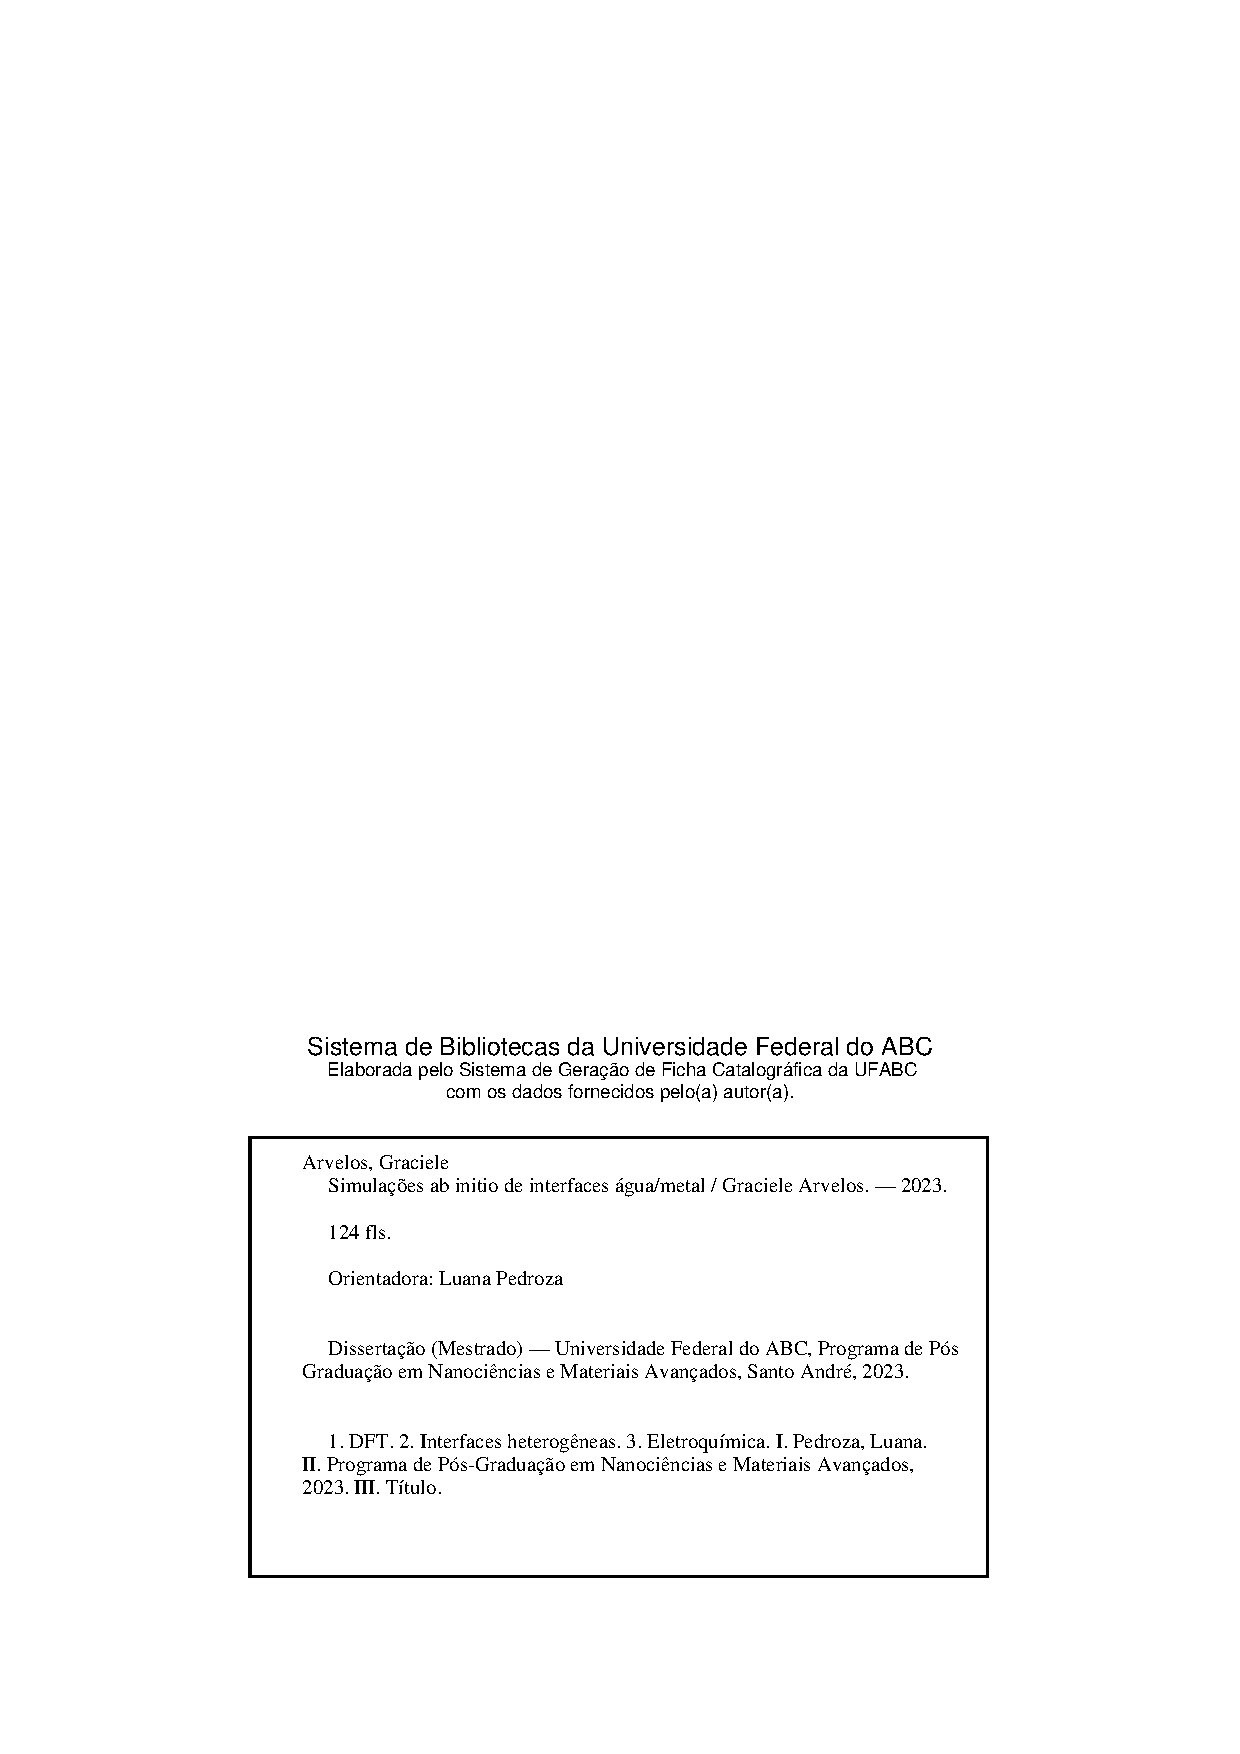
\includepdf{ficha.pdf}
\end{fichacatalografica}
%\begin{fichacatalografica}
%	\vspace*{\fill}					% Posição vertical
%	\hrule							% Linha horizontal
%	\begin{center}					% Minipage Centralizado
%	\begin{minipage}[c]{12.5cm}		% Largura
%	
%	\imprimirautor
%	
%	\hspace{0.5cm} \imprimirtitulo  / \imprimirautor. --
%	\imprimirlocal, \imprimirdata-
%	
%	\hspace{0.5cm} \pageref{LastPage} fls. : il.\\
%	
%	\hspace{0.5cm} \imprimirorientadorRotulo~\imprimirorientador\\
%	
%	\hspace{0.5cm}
%	\parbox[t]{\textwidth}{\imprimirtipotrabalho~--~\imprimirinstituicao,
%	\imprimirdata.}\\
%	
%	\hspace{0.5cm}
%		1. DFT.
%		2. Interfaces heterogêneas.
%		3. Eletroquímica.
%		I.  Pedroza, Luana Sucupira.
%		II. Universidade Federal do ABC.
%		III. Programa de Pós-Graduação em Nanociências e Materiais Avançados.
%		IV. Simulações \textit{ab initio} de interface água/metal \\ 			
%	
%	\hspace{8.75cm}\\
%	
%	\end{minipage}
%	\end{center}
%	\hrule
%\end{fichacatalografica}
% ---
% ---

% ---
% Inserir errata
% ---
% Isto é um exemplo de errata:


\begin{center}
	{\LARGE \textbf{Declaração de Atendimento às Observações da Banca}}
\end{center}
\vspace{\onelineskip}


Este exemplar foi revisado e alterado em relação à versão original, de acordo com as observações levantadas pela banca examinadora no dia da defesa, sob responsabilidade única do(a) autor(a) e com a anuência do(a) (co)orientador(a).
%
%Referente à dissertação de Mestrado intitulada “Simulações \textit{ab initio} de interfaces água/metal”, realizada por Graciele Martins Arvelos, fevereiro de 2023.
%
%Na folha 59, a Figura 13 corresponde a: 
%
%\begin{figure}[h!]
%	\centering
%	\caption{(a) Diferenças de densidades de carga $\Delta\rho$ das camadas H-Down, H-Up e H-Down/Up na superfície de tamanho $6\times4\times4$ e calculadas com os funcionais PBE e VDW-BH. Para todos os casos, o valor da isosuperfície foi $1.20 \times10^{-3}\;e/\AA$, onde vermelho (azul) indica uma diminuição (aumento) da densidade de carga durante a adsorção. (b) $ \Delta\rho $ médio ao longo do eixo z para os funcionais PBE (linha sólida) e VDW-BH (linha tracejada). As linhas pontilhadas correspondem às posições da última camada metálica de Pd e às posições dos átomos O e H das moléculas \textit{flat-down} e \textit{up} (funcional PBE). \label{fig:errata}}
%	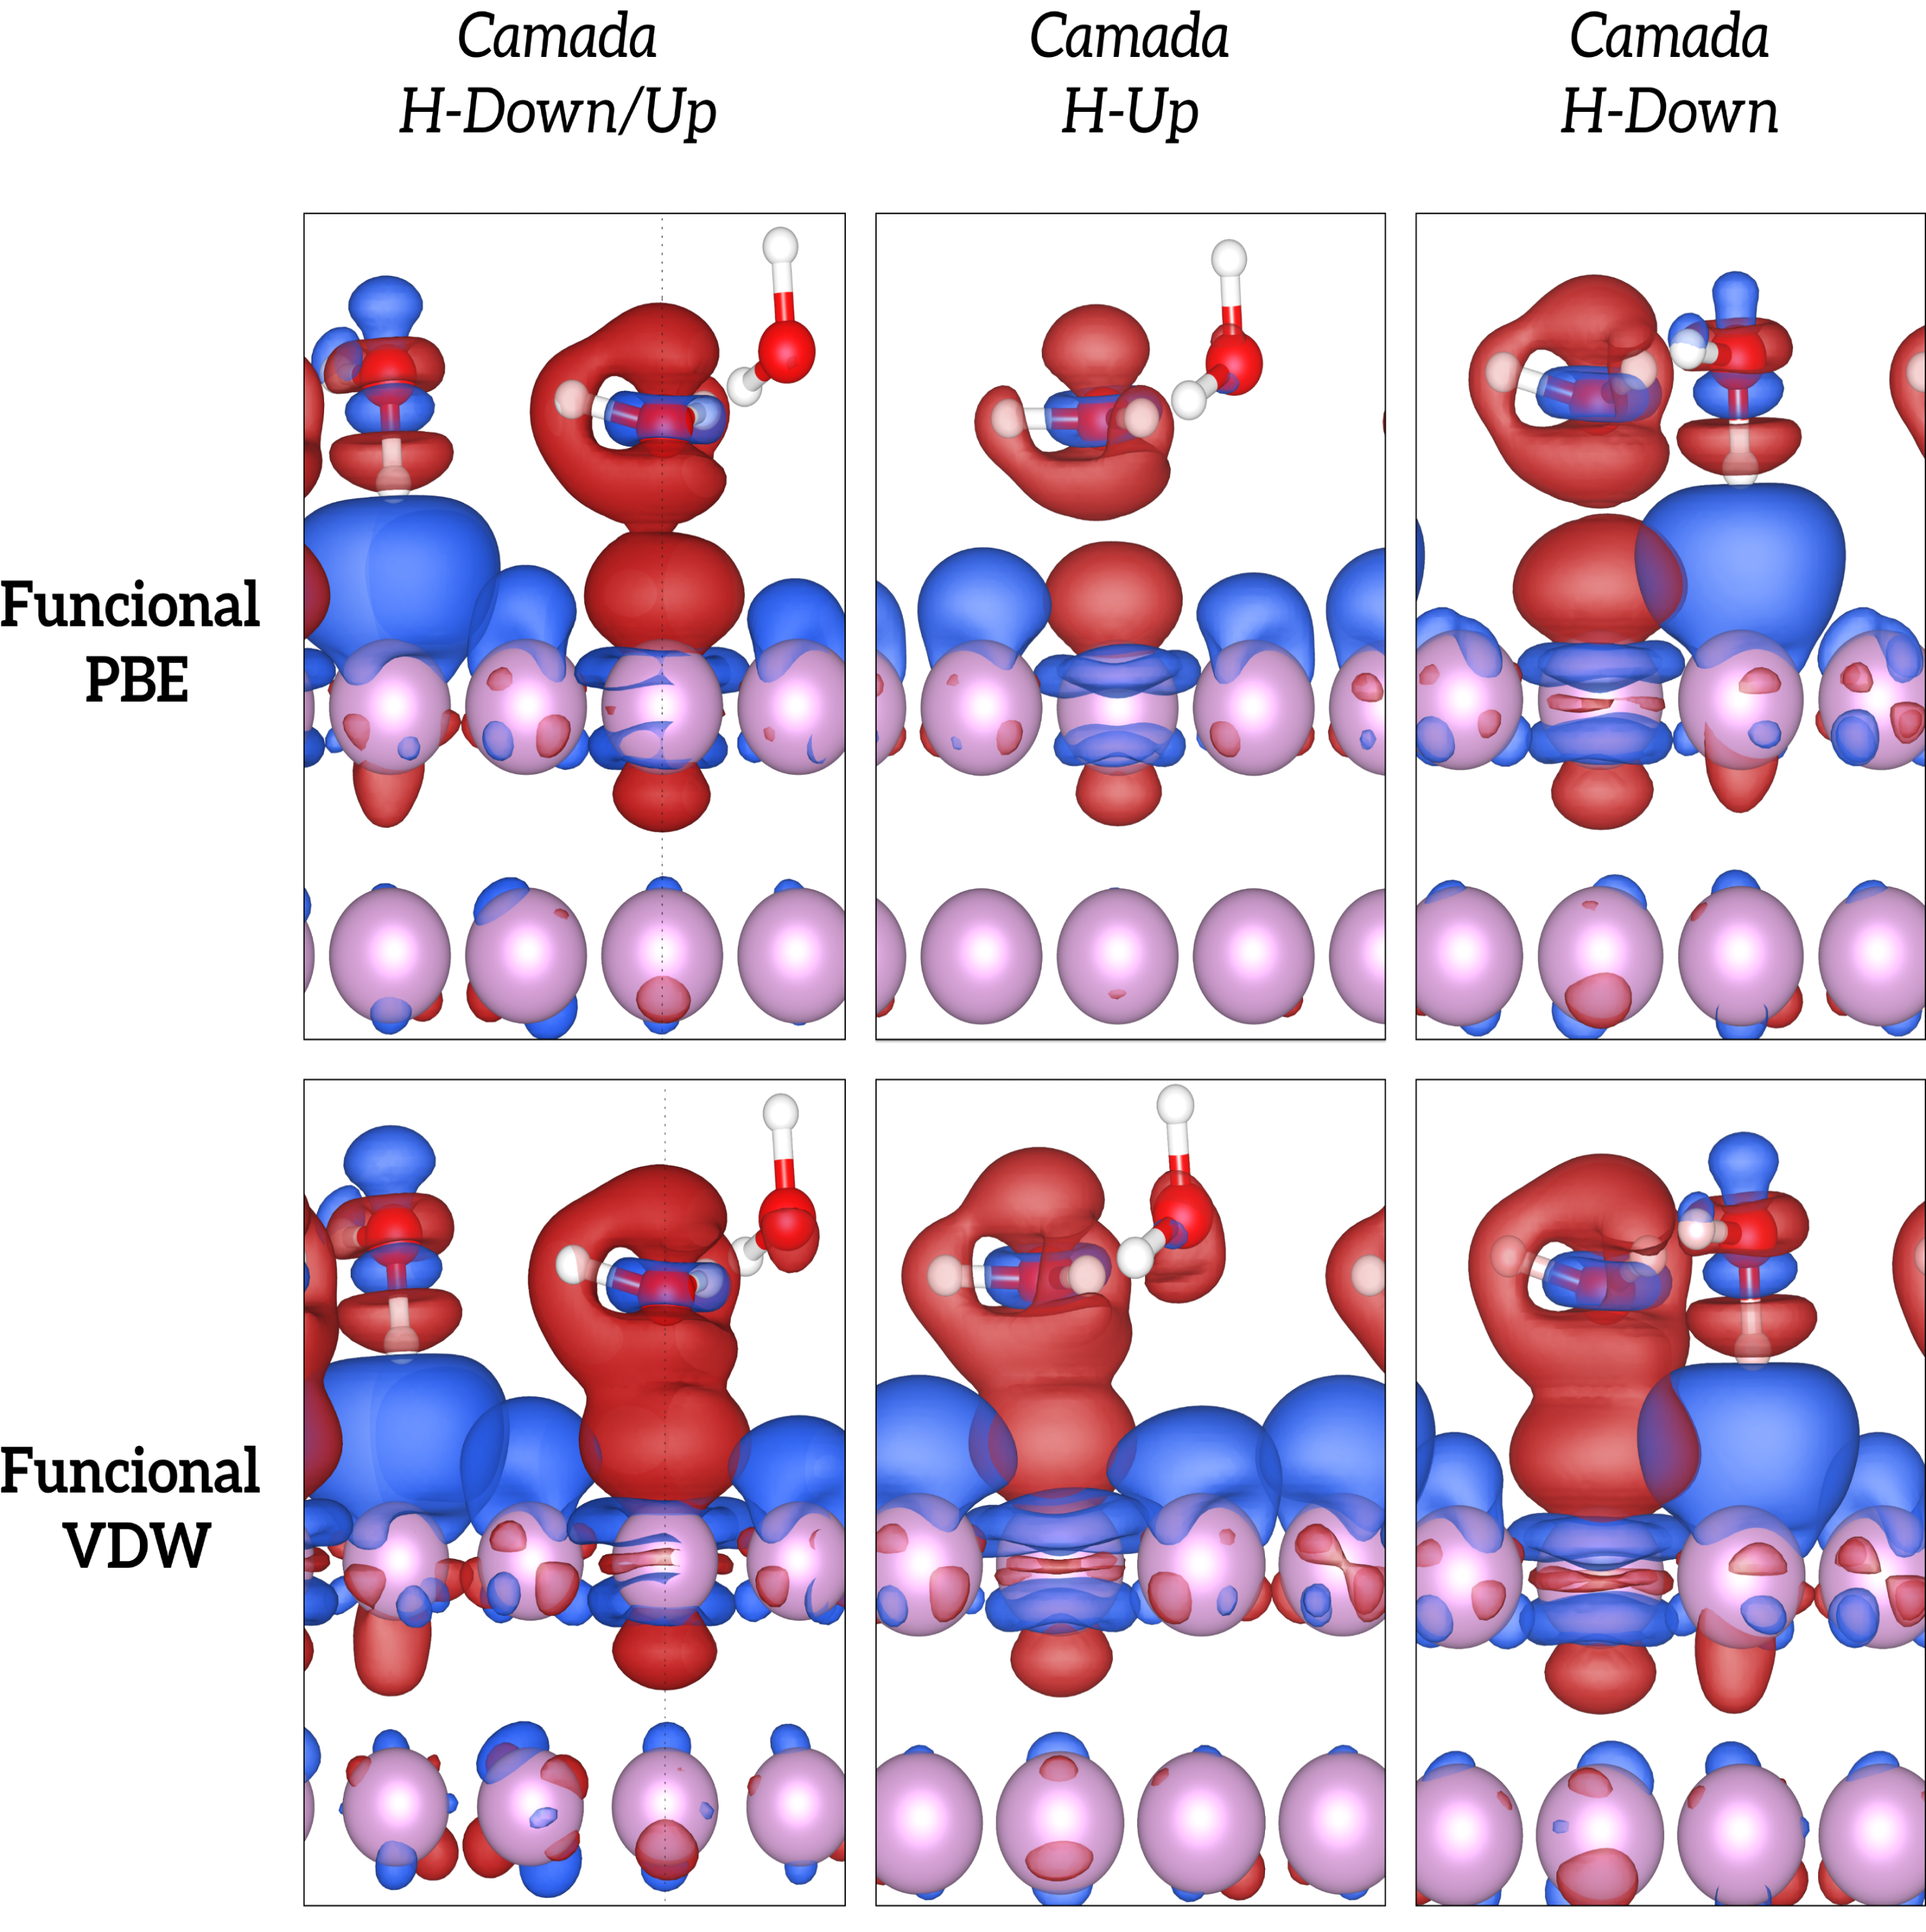
\includegraphics[scale=0.078]{figs/z_charge.png}
%	\legend{Fonte: Compilação da autora.}
%\end{figure}



 
% ---
%
% ---
% Inserir folha de aprovação
% ---
% Isto é um exemplo de Folha de aprovação, elemento obrigatório da NBR
% 14724/2011 (seção 4.2.1.3). Você pode utilizar este modelo até a aprovação
% do trabalho. Após isso, substitua todo o conteúdo deste arquivo por uma
% imagem da página assinada pela banca com o comando abaixo:
%
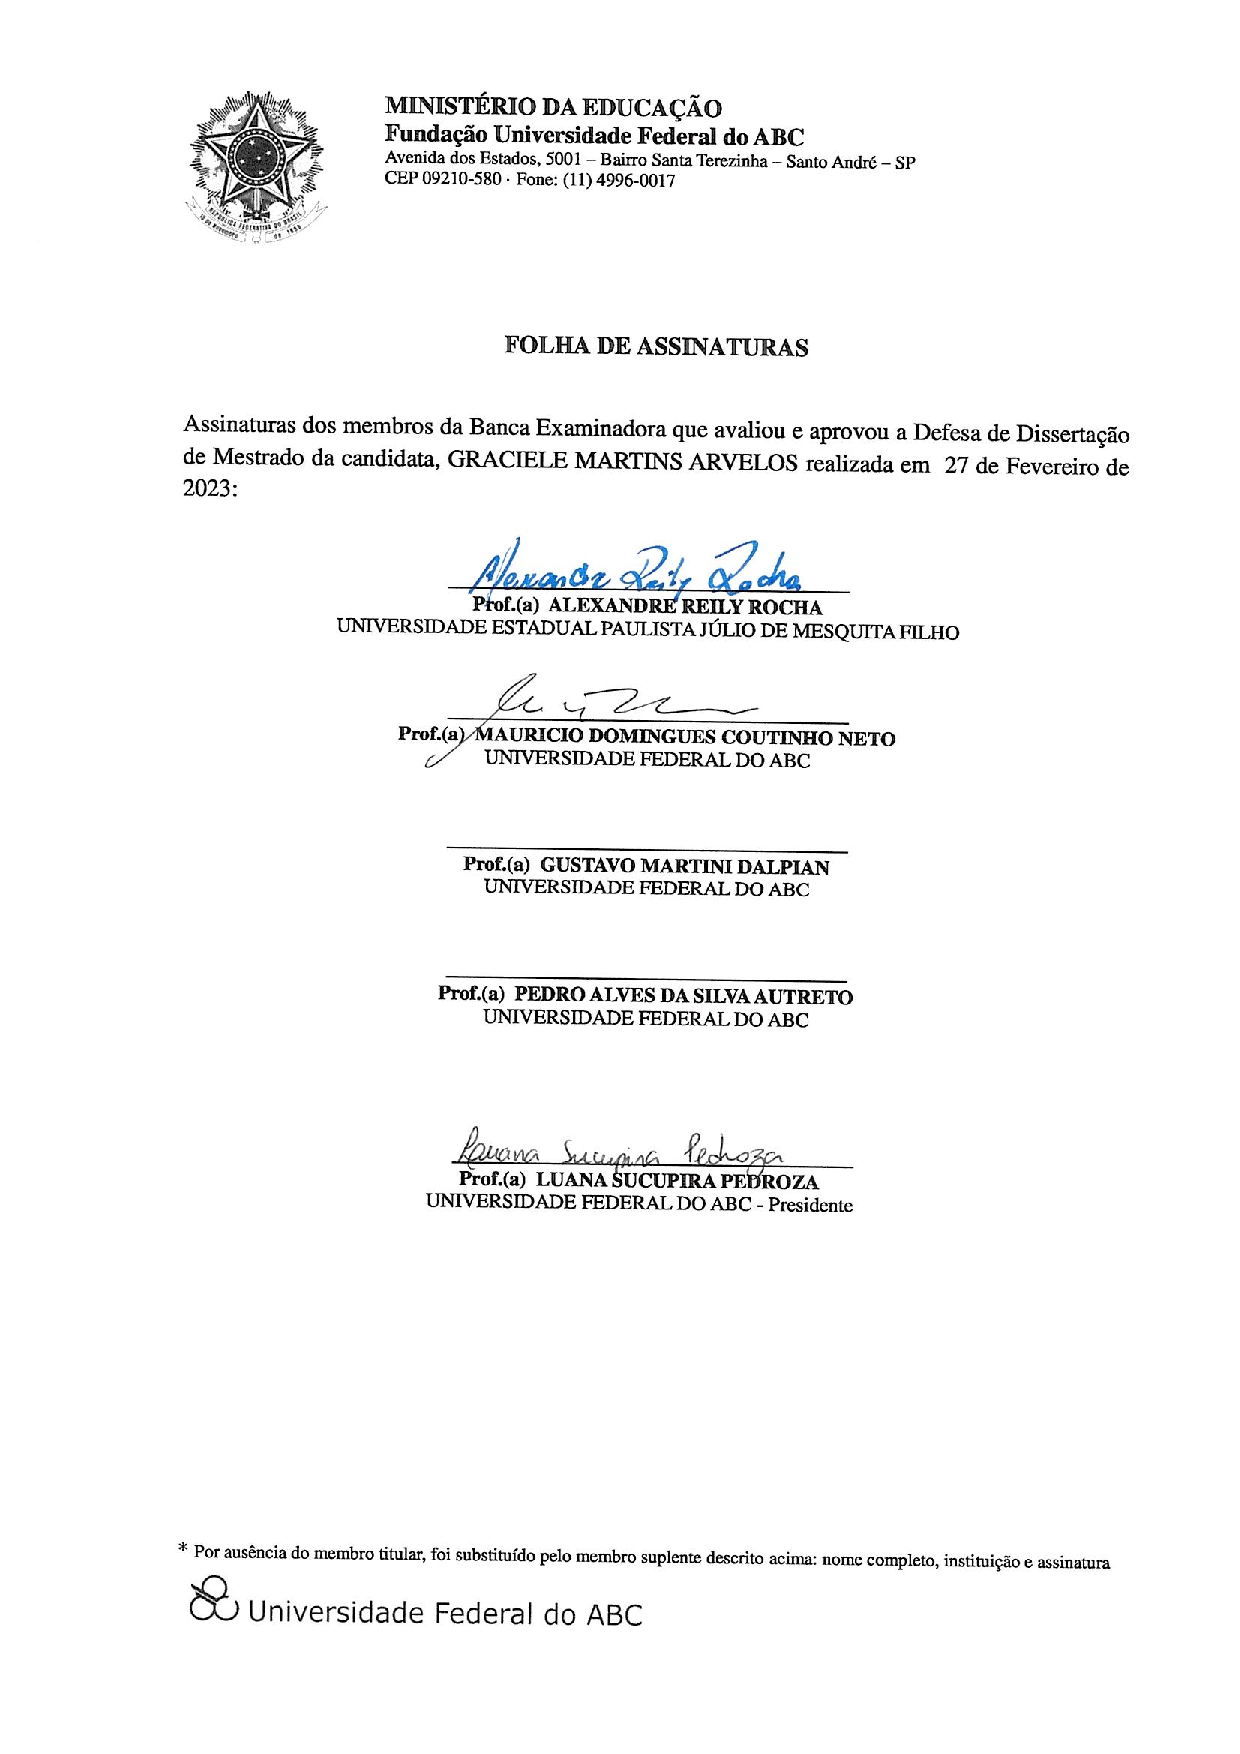
\includepdf{assinatura.pdf}
%



%\begin{folhadeaprovacao}
%
%  \begin{center}
%    {\ABNTEXchapterfont\large\imprimirautor}
%
%    \vspace*{\fill}\vspace*{\fill}
%    {\ABNTEXchapterfont\bfseries\Large\imprimirtitulo}
%    \vspace*{\fill}
%    
%    \hspace{.45\textwidth}
%    \begin{minipage}{.5\textwidth}
%        \imprimirpreambulo
%    \end{minipage}%
%    \vspace*{\fill}
%   \end{center}
%    
%   Trabalho aprovado. \imprimirlocal, \imprimirdata:
%
%   \assinatura{\textbf{\imprimirorientador} \\ Orientador} 
%   \assinatura{\textbf{Prof.$ \ulo $ Dr. Alexandre Reily Rocha}}
%   \assinatura{\textbf{Prof.$ \ulo $ Dr. Maurício Domingues Coutinho Neto}}
%   \assinatura{\textbf{Professor} \\ Convidado 3}
%   \assinatura{\textbf{Professor} \\ Convidado 4}
%      
%   \begin{center}
%    \vspace*{0.5cm}
%    {\large\imprimirlocal}
%    \par
%    {\large\imprimirdata}
%    \vspace*{1cm}
%  \end{center}
%  
%\end{folhadeaprovacao}
% ---
% ---


%% Agradecimento CAPES
% ---
% Dedicatória
% ---
\begin{dedicatoria}
   \vspace*{\fill}
   \centering
   \noindent
%   \textit{Dedico este trabalho ao meu pai que,\\
 %  por meio de frações somou a matemática à minha vida.} \vspace*{\fill}
   \textit{Dedico este trabalho a Telma Cristiane,\\ vítima da covid-19.} \vspace*{\fill}
\end{dedicatoria}
% ---

% ---
% Agradecimentos
% ---
\begin{agradecimentos}
Gostaria de agradecer, primeiramente, à duas pessoas que partiram, mas que honraram os anos aqui vividos amando aos seus intensamente: meu pai e Telma Cristiane. Meu pai, além do exemplo de integridade deixado como legado, foi o primeiro a despertar em mim a paixão pela ciência. Telma, com sua inteligência e irreverência marcou o coração e a vida de cada pessoa que a conheceu e assim, não somente marcou a minha vida, mas foi uma das bases que tornou possível esse momento. Sou imensamente grata por ter tido o privilégio de conviver e por ter sido amada profundamente por vocês. 

Agradeço à minha mãe pelo apoio incondicional e por ser esse porto seguro para nossa família. Aos meus irmãos Gustavo, Gabriel e Geovanna agradeço por terem me apoiado ao longo dessa jornada. Às minhas irmãs de coração Juliany, Sannya, Simone e Gabi: vocês personificam a cumplicidade, a parceria e a sinceridade que só se encontram numa amizade. Ao meu melhor amigo, companheiro e namorado Lucas, agradeço por todo suporte e por tirar minhas dúvidas de matemática. 

Agradeço aos meus avós de sangue e de coração: Iraci, Raymundo, Terezinha, Dinha, Dona Lica e Eunice. Vocês, com uma imensa sabedoria adquirida pelo passar dos anos, me revelam tesouros que só o tempo pode fornecer. Às minhas madrinhas Edevânia, Jovenilce e Josa, que sempre têm um sorriso caloroso e um abraço aconchegante a oferecer; aos meus tios Solimar, Junior e Ênio e às minhas tias Elaine, Cilene, Augusta Cássia, Ivonete Jesus por serem uma fonte de inspiração, força e perseverança. Aos meus primos Alynne, Priscyla, Mariane, Luís Eduardo, Carol, Douglas, João Victor, Anthônio, João Miguel e Emily pelo apoio e carinho. À Nicolly Eduarda por nos ensinar a acreditar. Às minhas amigas Iany, Cris e Érika por todos os conselhos e momentos compartilhados.

Sou profundamente grata pela experiência de ter sido aluna do Programa de Pós Graduação em Nanociências e em Materiais Avançados da UFABC. Agradeço em especial à minha orientadora Luana Pedroza pela paciência, dedicação, confiança e principalmente por ser uma inspiração e exemplo de pesquisadora. Ademais, agradeço aos professores Gustavo Dalpian, Celso Nishi, Alexandre Rocha e Antonio Pedroza pelo apoio e discussões ao longo desse trabalho.

Ao longo da minha jornada tive o privilégio de conviver com pessoas que admiro e que tornaram a caminhada mais leve. Agradeço aos meus amigos da UnB Ana Caroline e João Augusto, que mesmo longe foram fundamentais nessa etapa. Agradeço aos meus amigos da UFABC: Camila, Eduardo, Elton, Leo, Reinaldo, João e Café pelo companheirismo e por dividirem comigo as alegrias e desafios desse período na UFABC. 

O presente trabalho foi realizado com apoio da Coordenação de Aperfeiçoamento de Pessoal de Nível Superior - Brasil (CAPES) - Código de Financiamento 001 e pela Fundação de Amparo à Pesquisa do Estado de São Paulo (FAPESP) através da concessão de bolsa de estudo de Mestrado (processo nº 2020/16593-4) vinculado ao projeto Jovem Pesquisador nº 2017/10292-0. As opiniões, hipóteses e conclusões ou recomendações expressas neste material são de responsabilidade do(s) autor(es) e não necessariamente refletem a visão da FAPESP. 
\end{agradecimentos}
% ---

% ---
% Epígrafe
% ---
\begin{epigrafe}
    \vspace*{\fill}
	\begin{flushright}
		\textit{``Cada mulher sabe a força da natureza que abriga a torrente que flui de sua vida''\\
		(Itamar Vieira Junior)}
	\end{flushright}
\end{epigrafe}
% ---

% ---
% RESUMOS
% ---

% resumo em português
\begin{resumo}
 
%Contexto breve e problema investigado e não resolvido. Duas a três sentenças são suficientes

%Método breve e resultado mais importante

%Conclusões e implicações

Novas maneiras de geração de energia limpa estão relacionadas à reações que ocorrem em interfaces água/metal, por exemplo via processos eletroquímicos e de catálise heterogênea. Assim, a caracterização em nível atômico desses processos é fundamental para o aprimoramento das atuais e o desenvolvimento de novas fontes de energia renováveis. Para isso, é necessário compreender a estrutura e as propriedades eletrônicas de interfaces água/metal, bem como as respostas do sistema à aplicação de uma diferença de potencial externa. Para tanto, neste trabalho utilizou-se a Teoria do Funcional da Densidade (DFT) para caracterizar as interações de água (monômero e camada) em superfícies metálicas (Paládio e Ouro). Também utilizou-se o formalismo de Funções de Green Fora do Equilíbrio (NEGF) acoplado ao DFT para investigar o efeito da aplicação de um potencial externo sobre a interface água/metal e investigar como as propriedades estruturais, eletrônicas e vibracionais são alteradas. Assim, observamos que as moléculas tendem a se aproximarem do metal quando esse está carregado negativamente e se afastarem ao carregar positivamente. Essas alterações afetam as propriedades vibracionais e dependem fortemente da reatividade do metal.


%Aumentar a eficiência da conversão energética de células solares está ligado à melhoria dos processos eletroquímicos e de catálise heterogênea. Assim, a caracterização a nível atômico desses processos é fundamental para o aprimoramento das atuais e o desenvolvimento de novas fontes de energia renováveis. Para isso é necessário compreender a dinâmica e as propriedades eletrônicas da interface água/metal, bem como as respostas do sistema a pertubações externas. Para tanto, utilizou-se a Teoria do Funcional da Densidade (DFT) para caracterizar as interações provenientes do processo de adsorção da interface água/paládio, no qual foi considerado os efeitos das forças de dispersão através do funcional VDW-BH. Por meio da adsorção do monômero foi estudado como esse funcional fornece mais detalhes sobre o sistema e por meio da adsorção de uma camada de água observou-se que a interação água/metal melhora a ligação de hidrogênio e favorece a estabilidade da estrutura. Em posse dessas caracterizações, foi possível realizar cálculos preliminares da aplicação de um potencial externo sobre o sistema por meio formalismo de Funções de Green Fora do Equilíbrio (NEGF).

 \vspace{\onelineskip}
    
 \noindent
 \textbf{Palavras-chaves}:  DFT, interfaces heterogêneas, eletroquímica
\end{resumo}

% resumo em inglês
\begin{resumo}[Abstract]
 \begin{otherlanguage*}{english}
New ways of generating clean energy are related to reactions that occur at water/metal interfaces, for example via electrochemical and heterogeneous catalysis processes. Therefore, the characterization at the atomic level of these processes is fundamental for the improvement of the current ones and the development of new renewable energy sources. Thus, it is necessary to understand the structural and electronic properties of water/metal interfaces, as well as the system's responses to external perturbations. Therefore, in this work Density Functional Theory (DFT) was used to characterize the interactions of water (monomer and layer) on metallic surfaces (palladium and gold). The Non-Equilibrium Green's Function (NEGF) coupled to DFT was used in order to properly compute an external bias potential on the water/metal interface and to investigate how it affects the structural, electronic, and vibrational properties. Thus, we observe that the molecules tend to approach the metal when it is negatively charged and move away when it is positively charged. These changes affect the vibrational properties and are strongly dependent on the reactivity of the metal.




   \vspace{\onelineskip}
 
   \noindent 
   \textbf{Key-words}: DFT, heterogeneous interface, electrochemistry
   

 \end{otherlanguage*}
\end{resumo}

% resumo em francês 
%\begin{resumo}[Résumé]
 \begin{otherlanguage*}{french}
    Il s'agit d'un résumé en français.
 
   \vspace{\onelineskip}
 
   \noindent
   \textbf{Mots-clés}: latex. abntex. publication de textes.
 \end{otherlanguage*}
\end{resumo}

% resumo em espanhol
%\begin{resumo}[Resumen]
 \begin{otherlanguage*}{spanish}
   Este es el resumen en español.
  
   \vspace{\onelineskip}
 
   \noindent
   \textbf{Palabras clave}: latex. abntex. publicación de textos.
 \end{otherlanguage*}
\end{resumo}
% ---

% ---
% inserir lista de ilustrações
% ---
\pdfbookmark[0]{\listfigurename}{lof}
\listoffigures*
\cleardoublepage
% ---

% ---
% inserir lista de tabelas
% ---
\pdfbookmark[0]{\listtablename}{lot}
\listoftables*
\cleardoublepage
 ---

% ---
% inserir lista de abreviaturas e siglas
% ---
%\begin{siglas}
  \item[SI] Sistema Internacional de Unidades (\textit{Système international d'unités})
  \item[CNEN] Comissão Nacional de Energia Nuclear
  \item[IF] Instituto de Física
  \item[UnB] Universidade de Brasilia
\end{siglas}
% ---

% ---
% inserir lista de símbolos
% ---
%\begin{simbolos}
  \item[$ T $] temperatura
  \item[$ \tau $] torque, momento de força
  \item[$ \omega $] velocidade angular
  \item[$ \in $] pertence
\end{simbolos}
% ---

% ---
% inserir o sumario
% ---
\pdfbookmark[0]{\contentsname}{toc}
\tableofcontents*
\cleardoublepage
% ---



% ----------------------------------------------------------
% ELEMENTOS TEXTUAIS
% ----------------------------------------------------------
\textual

% ----------------------------------------------------------
% Introdução
% ----------------------------------------------------------
\chapter*[Introdução]{Introdução} 
\addcontentsline{toc}{chapter}{Introdução}

%Temas a serem abordados na introdução
%\begin{itemize}
%	\item Contextualização do problema: interesse e aplicações da interface água/metal. Isso inclui exemplos sobre aplicação em eletroquímica e catálise heterogênea;
%	\item Explicar sobre as propriedades do Paládio e o porquê dele está sendo utilizado;
%	\item Explicar como simulações pode ajudar no problema;
%	\item Explicar o objetivo principal do trabalho;	
%\end{itemize}
%\addcontentsline{toc}{chapter}{Introdução}
%, e principalmente descrevê-la em nível molecular, do rendimento 

Descrever atomisticamente a interface água/metal constitui um dos desafios na compreensão de processos eletroquímicos, de catálise heterogênea, resistência à corrosão e em processos catalíticos envolvendo células solares. Em particular, processos eletroquímicos envolvem a produção ou conversão de reações químicas em energia elétrica, de modo que para descrever e aperfeiçoar tais mecanismos é necessário considerar a aplicação de um potencial externo sobre o sistema. Assim, pesquisas envolvendo rotas alternativas de energias que diminuam o impacto ambiental estão relacionadas aos avanços e melhorias desses processos e, consequentemente implicam na descrição estrutural e dinâmica da interface água/metal de forma detalhada \cite{bias-pd,contex-nature}.   

%O que define a interface água/metal
Nesse sentido, as propriedades que caracterizam a reatividade e o comportamento eletroquímico da interface água/metal são definidas pela resposta da estrutura eletrônica em relação à fatores e perturbações externas, como por exemplo um potencial externo aplicado. Essas propriedades estão relacionadas aos arranjos atômicos definidos a partir das diversas orientações das moléculas de água, à formação de diferentes íons na interface e às diversas reações que podem ocorrer em diferentes potenciais \cite{bias-pd}. Em particular, considerando uma célula eletroquímica composta por dois reservatórios de carga que atuam como eletrodos e separados por uma solução eletrolítica, tem-se que, ao aplicar uma diferença de potencial, ocorre uma redistribuição de carga tanto na interface do eletrodo, quanto nos íons que compõem o eletrólito. Esse rearranjo leva à formação da dupla camada elétrica (\textit{electric double layer--EDL}) responsável pela formação e quebras de ligações químicas, e por processos de transferências de carga e adsorção que ocorrem na interface do eletrodo, como ilustrado na Figura \ref{fig:edl}. Assim, mesmo para eletrólitos mais concentrados as moléculas de água são dominantes nessa interface \cite{electro_curcinotta}. 


No entanto, descrever experimentalmente essa interface constitui um desafio experimental, uma vez que essas estruturas são analisadas em ultra vácuo e sob temperaturas criogênicas, o que impede de acompanhar a dinâmica de desordem e os efeitos de entropia da água líquida, bem como a influência de um potencial externo \cite{review-nature}. Dessa forma, técnicas estruturais e vibracionais têm sido utilizadas para investigar a interface água/metal ao longo das últimas décadas e revelado a dependência do comportamento das moléculas de água de acordo com o potencial externo \cite{rx1,rx2,sfg1,sfg2,sfg3,sfg_kramer,raman1,raman2}. Esse comportamento foi primeiramente observado por meio de espectroscopia de Raios-X (\textit{X-ray scattering}--XRS), a qual revelou um aumento da densidade interfacial de água em função do potencial \cite{rx1}. Além disso, \citeauthor{rx2} analisaram o efeito do potencial nas ligações de hidrogênio da interface acoplando simulações \textit{ab-initio} e espectros absorção de raios-X. 

%Os processos que ocorrem nessa interface estão diretamente ligados ao comportamento das moléculas de água na superfície metálica, como ilustrados na Figura \ref{fig:edl}.

%No âmbito experimental,
\begin{figure}[t!]
	\centering
	\caption{Ilustração de processos que podem ocorrer na interface eletroquímica ao aplicar uma diferença de potencial: (a) ausência e (b) presença da adsorção de espécies do eletrólito no metal; reações eletroquímicas que podem levar a (c) nucleação e formação de ligações químicas das espécies adsorvidas e (d)  modificações no eletrodo.}
	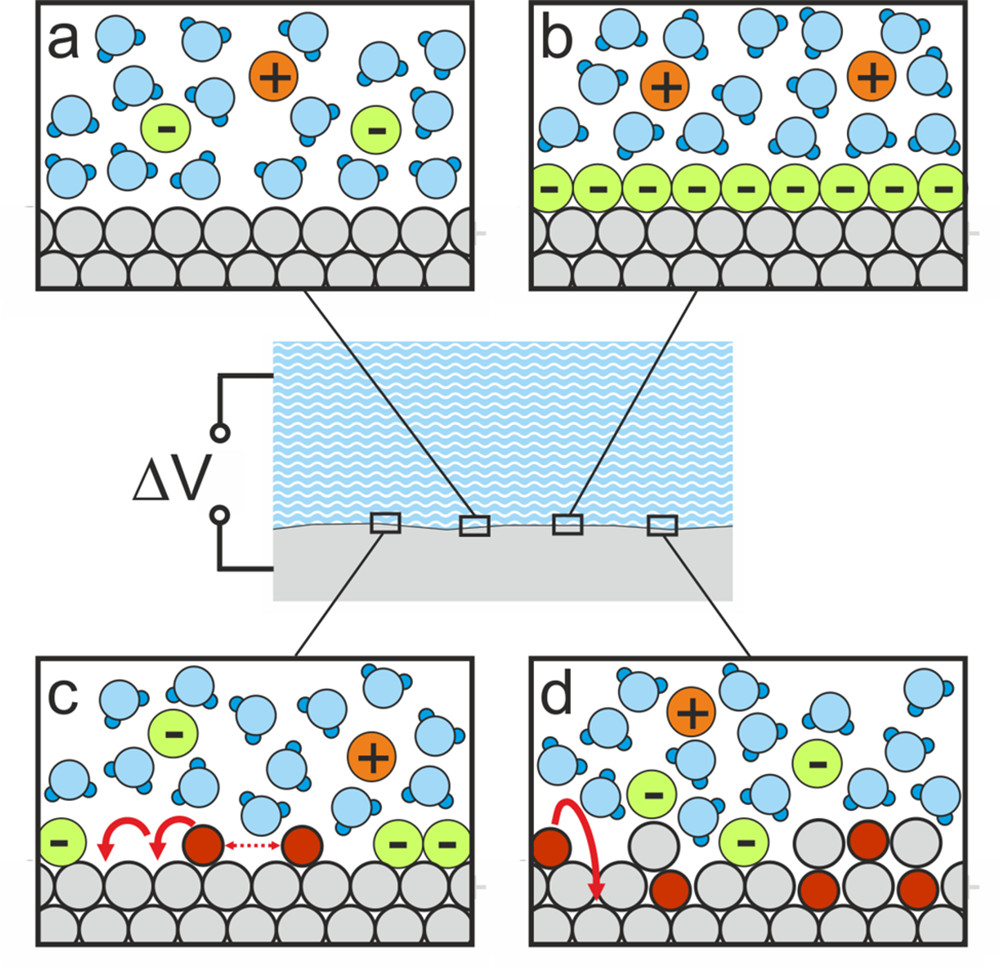
\includegraphics[scale=0.9]{figs/edl_figure.jpeg}
	\legend{Fonte: \citeauthor{edl_article}.}
	\label{fig:edl}
\end{figure}

As alterações estruturais provocadas pela variação do potencial externo é refletida nas propriedades vibracionais do sistema, como observado por meio da espectroscopia de absorção de radiação infravermelho (\textit{surface-enhanced infrared absorption spectroscopy}--SEIRAS) \cite{raman1}, o qual encontrou modificações no modo vibracional de deformação angular e um aumento do número de ligações de hidrogênio para potenciais positivos. Além disso, trabalhos de espectroscopia por Geração de Soma de Frequências (\textit{Sum frequency generation}--SFG), sensível somente à interface água/metal, identificou variações nas frequências mais altas de estiramento devido à variação do potencial e associaram tais modificações à ligações OH livre apontadas para o eletrodo de ouro, além de observarem uma fraca interação dessas moléculas com o metal \cite{sfg1,sfg2,sfg_kramer}. 


Em suma, resultados experimentais observam uma tendência das moléculas de se aproximarem (afastarem) do eletrodo para potenciais positivos (negativos). No entanto, os modelos experimentais apresentam resultados controversos e de difícil interpretação sobre a estrutura da água e além disso são sensíveis a modos vibracionais específicos. Dessa maneira, simulações computacionais têm sido fundamentais para analisar e descrever a nível atômico essas estruturas e auxiliar na interpretação de resultados experimentais. Em particular, a Teoria do Funcional da Densidade (DFT) têm elucidado questões experimentais em aberto, como no caso da estabilidade de estruturas de água adsorvidas em metais de transição \cite{michaedelis,monomer}. Nessa perspectiva, no Capítulo \ref{cap:denf} apresentaremos o formalismo da DFT e no Capítulo \ref{cap:equilibrio} a utilizaremos para abordar o problema da estabilidade de um monômero adsorvido em uma superfície metálica de paládio. Esse problema é revisitado  considerando o efeito de forças de dispersão de van der Waals através do funcional de troca e correlação VDW-BH \cite{vdw-bh}. Ainda nesse capítulo analisaremos o efeito da adsorção sobre as ligações de hidrogênio através das propriedades de uma camada de água adsorvida no metal. 


Apesar dos avanços teóricos obtidos via simulações DFT na elucidação de questões relacionadas à adsorção de estruturas de água no metal, outras questões cruciais permanecem em aberto. Por exemplo, o efeito de um potencial externo sobre a orientação das moléculas de água e como o potencial afeta as interações água/metal e as ligações de hidrogênio. Todavia, simular de forma realística esses processos é um desafio computacional, visto que não existe uma metodologia definida para descrever os componentes de uma célula eletroquímica e a superfície metálica carregada. Assim, a investigação do comportamento das moléculas de água nessa interface sob um potencial externo aplicado é fundamental para construir modelos mais realísticos dos processos que ocorrem nessa interface, uma vez que essas propriedades são fundamentais para compreender o rearranjo estrutural, oxidação e redução, além de transferências de carga que ocorrem nessa região \cite{electro_curcinotta,bias_agua1}.

%Entretanto, a modelagem computacional de processos eletroquímicos possui elevado custo, pois requerem a descrição da superfície carregada e as espécies que compõem o eletrólito e não existe uma abordagem unificada sobre como descrever tais estruturas \cite{electro_curcinotta}. Como resultado, 


Nesse sentido, um dos primeiros estudos que investigou o efeito de superfícies metálicas carregadas sobre estruturas de água utilizou simulações empíricas de dinâmica molecular clássica, no qual a eletrização da superfície metálica do eletrodo era alcançada por meio de cargas induzidas nos átomos do eletrodo \cite{charge1}. No âmbito da DFT, \citeauthor{bias-pd} implementou a eletrização de uma superfície metálica por meio da variação de elétrons no eletrodo e a diferença de potencial era introduzida por meio de uma camada de vácuo entre as moléculas da solução e comparado com um potencial de referência artificial (eletrodo de hidrogênio). Com essa abordagem, estudou-se a resposta da polarização da interface água/Pd(111) e água/Cu(111) em relação a um potencial externo \cite{charge2,bias-pd}. Outras implementações nesse sentido surgiram na literatura ao longo dos anos e forneceram detalhes da interface água/metal, bem como os efeitos de polarização, detalhes sobre processos que ocorrem na EDL e informações sobre energias de ativação \cite{hydrogen2,hydrogen1,hydrogen3,hydrogen4,hydrogen5}. No entanto, esses modelos controlam o potencial aplicado a partir da carga adicionada ou subtraída do eletrodo, ao passo que, nos experimentos o que se controla é o potencial aplicado.

Nesse sentido, \citeauthor{artigo-luana} propuseram utilizar o formalismo de Funções de Green Fora do Equilíbrio (\textit{Non--Equilibrium Green’s Function--NEGF}) para investigar processos eletroquímicos. Com isso, os autores observaram o comportamento dependente da molécula de água em relação ao potencial externo aplicado e analisaram como a posição de mínimo é afetada pelo potencial externo. Essa abordagem permite controlar o potencial aplicado aos eletrodos sem alterar a carga total do sistema. Além disso, essa metodologia trata todos os elementos que compõem um sistema eletroquímico ao nível atomístico. Isso permite acompanhar com mais acurácia as interações e trocas de carga que ocorrem na interface entre a água e o metal. 

%Utilizar simulações para entender esses sistemas. Descrever sobre trabalhos anteriorea no tema e os avanços alcançados. Aqui falar sobre o trabalho pioneiro do Michaedelis.  Em face das dificuldades de se caracterizar experimentalmente a interface água/ metal, os cálculos utilizando



%Tendo em vista o potencial de aplicação que uma descrição atomística pode fornecer, escolhemos estudar a interface água/Pd visto que o Paládio é mais reativo que outros metais platinados e possui grande afinidade em relação às ligações envolvendo hidrogênio e oxigênio \cite{paladio}. Isso posto, nesse trabalho realizaremos a caracterização detalhada da interface água/Pd utilizando dois funcionais distintos: GGA-PBE e VDW-BH\cite{vdw-bh}. 

Isso posto, nesse trabalho utilizamos o formalismo de Funções de Green Fora do Equilíbrio (\textit{Non-Equilibrium Green's Function} -- NEGF) para aplicar uma diferença de potencial sobre eletrodos metálicos e assim, descrever atomisticamente o efeito das superfícies carregadas sobre estruturas de água (monômero e camada) adsorvidas no metal. Para isso, aplicamos a diferença de potencial externa a dois eletrodos metálicos com características reativas distintas: Au(111) e Pd(111). O ouro é considerado um metal hidrofóbico e se destaca pela atividade eletroquímica, ao passo que o paládio é um metal mais reativo e hidrofílico. 

Dessa forma, através do formalismo NEGF conseguimos caracterizar e comparar o efeito do potencial sobre o comportamento reativo de estruturas de água adsorvidas nesses metais. Assim, no Capítulo \ref{cap:green} apresentaremos os detalhes sobre a modelagem desses sistemas no âmbito do formalismo de NEGF, além de como calcular a força atômica em problemas fora do equilíbrio, ao passo que, no Capítulo \ref{cap:bias} apresentaremos o efeito do potencial sobre as propriedades eletrônicas, estruturais e vibracionais dessas estruturas de água adsorvidas.

Considerando a caracterização da interface água/metal, primeiramente obteremos as propriedades de adsorção da água no metal. Além disso, analisaremos o papel das forças de dispersão em descrever as interações água/metal e ligações de hidrogênio. Em seguida, através da aplicação de um potencial externo sobre estruturas de água adsorvidas em superfícies metálicas, esperamos obter detalhes sobre o comportamento das moléculas em superfícies metálicas carregadas além do efeito do potencial sobre as interações água/metal e sobre as ligações de hidrogênio. Com essas caracterizações, esperamos descrever de forma mais realística um modelo protótipo de uma célula eletroquímica.

% constituem um desafio  s avanços obtidos para descrever  simular situações realísticas do rearranjo estrutural que ocorre na interface de uma célula eletroquímica sob a aplicação de um potencial externo é um desafio computacional. considerando   A dificuldade em investigar moléculas de água isoladas adsorvidas no metal é devido à tendência da molécula em formar ligações de hidrogênio e clusters. Entretanto, através do trabalho conduzido por \citeauthor{michaedelis} em \citeyear{michaedelis}, no qual foi utilizada a , revelou-se que a orientação mais estável do monômero é aquela cujo  o dipolo fica paralelo ao metal (\emph{flat}) e no sítio \textit{atop}, visto que essa orientação favorece a interação do orbital molecular $b_1$ com o substrato \cite{review-nature}. Esse trabalho foi pioneiro ao utilizar simulações \textit{ab initio} para descrever a interface água/sólido por meio de funcionais semi-locais da família GGA, de modo que a partir dele vários outros trabalhos foram realizados utilizando funcionais semi-locais e inclusive, apresentaram divergências em relação às propriedades eletrônicas e geométricas \cite{review-nature}\cite{review}\cite{review2}.

%Além disso, cálculos DFT possibilitaram estudar a estabilidade, sítios de adsorção e configurações atômicas de uma gama de estruturas adsorvidas em metais, tais como clusters, cadeias unidimensionais, camadas bidimensionais e estruturas tridimensionais \cite{monomer} \cite{review}; não obstante, tais estudos forneceram detalhes das interações água-metal e a relação dessas interações com as ligações de hidrogênio \cite{adrien}. Os avanços teóricos obtidos via simulações DFT e outros métodos computacionais, concomitantemente com a melhoria e o surgimento de técnicas experimentais, elucidaram várias questões \cite{review}. No entanto, outras permanecem em aberto, tais como a orientação das moléculas de água em camadas bidimensionais, bem como a validade do modelo de bicamada (\textit{bilayer}) amplamente utilizado; a importância do número de ligações de hidrogênio na estabilidade de clusters e camadas e principalmente, a validade das comparações entre cálculos teóricos e em relação aos resultados experimentais. 

%Falar sobre as limitações existentes. Em seguida falar sobre a inverstigação desses sistemas utilizando funcionais do tipo vdw o trabalho do Adrien - Solução.
%Em particular, esse último questionamento está atrelado à escolha do funcional de troca, à correlação nos cálculos de DFT e à sensibilidade dessa escolha ao descrever as interações existentes no sistema. De modo geral, o funcional mais reportado na literatura  e mais utilizado na descrição das propriedades eletrônicas e geométricas da interface água/metal  é o funcional semi local GGA-PBE\cite{PBE}. Todavia, esse funcional não inclui correlações não locais e não considera forças de dispersão de van der Waals, que são relevantes na descrição da interação água- metal e água- água. Apesar disso, o funcional PBE fornece informações estruturais e propriedades geométricas próximas às obtidas com os funcionais do tipo vdW, o que explica o sucesso desse funcional em descrever esses sistemas estruturalmente \cite{vdw-func} \cite{adrien}.


%Falar o que o meu trabalho se propõe e a divisão do texto.




%Dessa forma, no Capítulo \ref{cap:denf} serão apresentados os fundamentos sobre a Teoria do Funcional da Densidade, junto aos detalhes sobre os funcionais PBE e VDW. Em seguida, no Capítulo \ref{cap:green} abordaremos o formalismo das Funções de Green fora do Equilíbrio utilizado para estudar um potencial externo aplicado ao sistema. No Capítulo \ref{cap:metodologia} serão descritos os detalhes computacionais, bem como os resultados e as discussões. Por fim, no Capítulo \ref{cap:conclusao} traremos as principais conclusões do trabalho e as perspectivas futuras.


%%Contextualização do problema
%Compreender atomicamente a interface água/metal, e principalmente descrevê-la em nível molecular, constitui um dos desafios no aumento do rendimento de processos eletroquímicos, de catálise heterogênea, resistência à corrosão e eletrocatálise \cite{contex-nature}. Em particular, pesquisas envolvendo rotas de energias renováveis que diminuam o impacto ambiental estão relacionadas à descrição estrutural e dinâmica da interface eletrodo/eletrólito sujeita a perturbações externas, como por exemplo a aplicação de uma diferença de potencial \cite{bias-pd,review-nature}. Isso ocorre pois a resposta eletroquímica é resultado dos arranjos moleculares da água na superfície carregada e do efeito das perturbações externas sobre as ligações de hidrogênio e as interações entre a água e o eletrodo \cite{bias_electro_cucinotta,bias_electrochemistry}. 
%
%%\todo[inline]{falar que métodos vibracionais foram usados para investigar a estrutura}
%%Desafios experimentais + limitações dos resultados experimentais envolvendo BIAS
%
%
%Um dos desafios de se caracterizar experimentalmente esses sistemas constitui em analisar esses substratos em ultra vácuo-- \textit{ultra-high vacuum} (UHV)--sob temperaturas criogênicas (abaixo de 200 K). Consequentemente, as estruturas obtidas não revelam a dinâmica de desordem e os efeitos de entropia da água líquida, muito menos consideram perturbações externas. Assim, simulações computacionais têm sido fundamentais para analisar e descrever a nível atômico essas estruturas e principalmente auxiliar na interpretação de resultados experimentais\cite{review,review2}. A título de exemplo, cálculos de estrutura eletrônica utilizando a Teoria do Funcional da Densidade (DFT) complementaram resultados experimentais sobre a orientação mais estável de um monômero adsorvido no metal e revelaram que a orientação paralela à superfície metálica (\textit{flat}) favorece a interação do mais alto orbital molecular da água com o substrato \cite{review-nature}. Em especial, esse trabalho foi pioneiro ao utilizar simulações \textit{ab initio} para descrever a interface água/sólido por meio de funcionais semi-locais da família GGA e motivou a investigação de sistemas mais complexos, como processos de dissociação em camadas de água no metal \cite{layer,monomer}.
%
%No entanto, apesar dos avanços obtidos ao analisar estruturas adsorvidas no metal em UHV, não existe um consenso sobre o arranjo estrutural da água em superfície metálicas carregadas. Nesse sentido, técnicas experimentais estruturais e vibracionais têm sido utilizadas para investigar a interface água/metal ao longo das últimas décadas e revelado a dependência do comportamento das moléculas de água de acordo com o potencial externo \cite{rx1,rx2,sfg1,sfg2,sfg3,sfg_kramer,raman1,raman2}. Esse comportamento foi primeiramente observado por meio de espectroscopia de Raios-X (\textit{X-ray scattering}--XRS), o qual revelou um aumento da densidade interfacial de água para potenciais positivos \cite{rx1}. Além disso, \citeauthor{rx2} analisaram o efeito do potencial nas ligações de hidrogênio da interface acoplando simulações \textit{ab-initio} e espectros absorção de raios-X. Apesar dos autores observarem diversas orientações nas simulações, nos espectros identificaram apenas estruturas paralelas à superfície, no qual uma ligação OH participava de uma ligação de hidrogênio e a outra ficava livre. 
%
%As alterações estruturais provocadas pela variação do potencial externo é refletida nas propriedades vibracionais do sistema, como observado por meio da espectroscopia de absorção de radiação infravermelho (\textit{surface-enhanced infrared absorption spectroscopy}--SEIRAS) \cite{raman1}, o qual encontrou modificações no modo vibracional \textit{bending} e um aumento do número de ligações de hidrogênio indo de potenciais negativo para positivos. Além disso, espectroscopia por Geração de Soma de Frequências (\textit{Sum frequency generation}--SFG), sensível somente à interface água/metal, identificaram variações nas frequências mais altas de estiramento devido à variação do potencial e associaram tais modificações à ligações OH livre apontadas para o eletrodo de ouro, além de observarem uma fraca interação dessas moléculas com o metal \cite{sfg1,sfg2,sfg_kramer}. 
%
%
%Em suma, resultados experimentais observam uma tendência das moléculas de se aproximarem (afastarem) do eletrodo para potenciais positivos (negativos). No entanto, os modelos experimentais ou apresentam resultados controversos sobre a estrutura da água ou são sensíveis a estruturas ou vibrações específicas. Isso posto, simulações computacionais são fundamentais para complementar e auxiliar na interpretação de resultados experimentais, uma vez que permite identificar estruturas cuja sensibilidade dos experimentos não captam \cite{simulacao_vibrational}. Entretanto, a modelagem computacional de processos eletroquímicos possui elevado custo, pois requerem a descrição da superfície carregada e as espécies que compõem o eletrólito e não existe uma abordagem unificada sobre como descrever tais estruturas \cite{electro_curcinotta}. Em geral, o efeito do potencial sobre o eletrodo é aplicado alterando-se a carga total do sistema através da adição ou subtração de íons no sistema (REF). No entanto, tais métodos dificultam a comparação com experimentos, uma vez que experimentalmente o potencial que é de fato controlado. Além disso, outros trabalhos reportam a utilização de um eletrodo de hidrogênio padrão (\textit{Standard Hydrogen Electrode}--SHE) computacional (REF), todavia, para metais como o Pd (111) esse método apresenta uma divergência de 0.8 eV do valor experimental para o valor do potencial de carga zero. 
%
%Nesse sentido, \citeauthor{artigo-luana} propuseram utilizar o formalismo de Funções de Green Fora do Equilíbrio (\textit{Non-Equilibrium Green’s Function}--NEGF) para estudar um protótipo de uma célula eletroquímica, no qual uma diferença de potencial é aplicada num monômero adsorvido numa superfície metálica de Au(111). Essa abordagem possui a vantagem de controlar o potencial aplicado diretamente e não alterar a carga total do sistema. Além disso, todos os componentes do sistema são modelados atomisticamente. Assim, os autores observaram que a molécula tende a se aproximar da superfície metálica carregada positivamente e se afasta para a superfície negativa, em consonância com achados experimentais. Apesar do estudo fornecer detalhes sobre o comportamento estrutural da molécula de água adsorvida no metal sob um potencial externo no âmbito atomístico e propor uma nova abordagem para investigar processos eletroquímicos, os autores não investigaram o efeito da superfície carregada sobre as propriedades vibracionais e sobre as ligações de hidrogênio.
%
% 
%
% Assim, no Capítulo \ref{cap:denf} abordaremos detalhes sobre a DFT e no Capítulo \ref{cap:equilibrio} revisitaremos o problema do monômero adsorvido no metal e também a estabilidade de uma camada de água adsorvida.
%
%\todo[inline,color=green!40]{objetivo do trabalho}


% Experimento de RX. IR. SGF. Apesar de fornecer 


% Em muitos casos elucidou questões experimentais em aberto, como nos casos do sítio de adsorção e da orientação do monômero de água em metais. A dificuldade em investigar moléculas de água isoladas adsorvidas no metal é devido à tendência da molécula em formar ligações de hidrogênio e clusters. Entretanto, através do trabalho conduzido por \citeauthor{michaedelis} em \citeyear{michaedelis}, no qual foi utilizada a Teoria do Funcional da Densidade (DFT), revelou-se que a orientação mais estável do monômero é aquela cujo  o dipolo fica paralelo ao metal (\emph{flat}) e no sítio \textit{atop}, visto que essa orientação favorece a interação do orbital molecular $b_1$ com o substrato \cite{review-nature}. 

%Além disso, cálculos DFT possibilitaram estudar a estabilidade, sítios de adsorção e configurações atômicas de uma gama de estruturas adsorvidas em metais, tais como clusters, cadeias unidimensionais, camadas bidimensionais e estruturas tridimensionais \cite{monomer,review}; não obstante, tais estudos forneceram detalhes das interações água-metal e a relação dessas interações com as ligações de hidrogênio \cite{adrien}. Os avanços teóricos obtidos via simulações DFT e outros métodos computacionais, concomitantemente com a melhoria e o surgimento de técnicas experimentais, elucidaram várias questões \cite{review}. No entanto, outras permanecem em aberto, tais como a orientação das moléculas de água em camadas bidimensionais, bem como a validade do modelo de bicamada (\textit{bilayer}) amplamente utilizado; a importância do número de ligações de hidrogênio na estabilidade de clusters e camadas e principalmente, a validade das comparações entre cálculos teóricos e em relação aos resultados experimentais. 


%Em particular, esse último questionamento está atrelado à escolha do funcional de troca, à correlação nos cálculos de DFT e à sensibilidade dessa escolha ao descrever as interações existentes no sistema. De modo geral, o funcional mais reportado na literatura  e mais utilizado na descrição das propriedades eletrônicas e geométricas da interface água/metal  é o funcional semi local GGA-PBE \cite{PBE}. Todavia, esse funcional não inclui correlações não locais e não considera forças de dispersão de van der Waals, que são relevantes na descrição da interação água- metal e água- água. Apesar disso, o funcional PBE fornece informações estruturais e propriedades geométricas próximas às obtidas com os funcionais do tipo vdW, o que explica o sucesso desse funcional em descrever esses sistemas estruturalmente \cite{vdw-func,adrien}.


%Falar o que o meu trabalho se propõe e a divisão do texto.
%Tendo em vista o potencial de aplicação que uma descrição atomística pode fornecer, escolhemos estudar a interface água/Pd visto que o Paládio é mais reativo que outros metais platinados e possui grande afinidade em relação às ligações envolvendo hidrogênio e oxigênio \cite{paladio}. Isso posto, nesse trabalho realizaremos a caracterização detalhada da interface água/Pd utilizando dois funcionais distintos: GGA-PBE e VDW-BH\cite{vdw-bh}. Isso se dará pelo cálculo da energia de adsorção, obtenção das propriedades geométricas e vibracionais de um monômero e de uma camada de água adsorvidas no Pd. 

%Considerando a adsorção do monômero de água, esperamos obter informações atomísticas sobre a interação água-metal e principalmente, o papel das forças de dispersão em descrever essas interações por meio do funcional do tipo VDW. Em seguida, estudando um sistema maior e mais complexo - a camada de água - serão analisadas as ligações de hidrogênio entre as moléculas de água e a relação dessas interações com metal.

%Dessa forma, no Capítulo \ref{cap:denf} serão apresentados os fundamentos sobre a Teoria do Funcional da Densidade, junto aos detalhes sobre os funcionais PBE e VDW. Em seguida, no Capítulo \ref{cap:green} abordaremos o formalismo das Funções de Green fora do Equilíbrio utilizado para estudar um potencial externo aplicado ao sistema. No Capítulo \ref{cap:metodologia} serão descritos os detalhes computacionais, bem como os resultados e as discussões.% Por fim, no Capítulo \ref{cap:conclusao} traremos as principais conclusões do trabalho e as perspectivas futuras.

% ----------------------------------------------------------
% PARTE - preparação da pesquisa
% ----------------------------------------------------------
\part{Fundamentos Teóricos}

% ---
% Capitulos:
% ---

\chapter{Teoria do Funcional da Densidade\label{cap:denf}}

A descrição atomística das interações água/sólido fornece informações da natureza das ligações. Para lidar com essa escala de caracterização é necessário tratar os átomos e moléculas no âmbito da Mecânica Quântica. Isso implica obter a função de onda de um sistema de N elétrons por meio da solução da Equação de Schr\"{o}dinger, o que é inviável de se obter analiticamente. Nesse sentido, a Teoria do Funcional da Densidade (\textit{Density Functional Theory}--DFT) emerge como um eficiente método para a descrição das propriedades estruturais e eletrônicas do sistema a partir da densidade eletrônica.

Nesse capítulo serão apresentados os fundamentos da Teoria do Funcional da Densidade, abrangendo desde o advento dessa Teoria em 1964 por meio dos \textit{Teoremas de Hohenberg-Kohn} (Seção \ref{teoremas}) até os esforços atuais em desenvolver Funcionais de Troca e correlação não locais que incluam forças de dispersão. A principal implicação desses teoremas é a possibilidade de reescrever a Equação de  Schr\"{o}dinger de um sistema de N elétrons em função da densidade eletrônica, como foi realizado pelas \textit{Equações de Kohn-Sham}. Essa abordagem e as principais aproximações para o termo de troca e correlação serão descritas na Seção \ref{kohn}.


\section{Teoremas de Hohenberg-Kohn\label{teoremas}}

A \textit{Densidade Eletrônica} é uma quantidade fundamental no desenvolvimento da Teoria do Funcional da Densidade. Para tanto, um sistema que possua N elétrons, tem a densidade eletrônica definida como:
\begin{equation}\label{eq:rho}
	\dens=eN\int\abs{\Psi(\vb{r},\vb{r}_2,\ldots,\vb{r}_N)}^2 \dd{\vb{r}_2},\ldots,\dd{\vb{r}_N}. 
\end{equation}  

De acordo com a interpretação usual da Mecânica Quântica $ \Psi^{\ast}(\vb{r})\Psi(\vb{r}) $ é definida como a Densidade de Probabilidade de encontrar um elétron no qual o estado físico num certo instante é determinado pela Função Onda $ \Psi(\vb{r}) $. Logo, segue que a Densidade Eletrônica representa a Densidade de Probabilidade de encontrar um elétron na posição $ \vb{r} $ independente da posição dos outros N-1 elétrons. 

No sistema de N elétrons a interação \textit{elétron-elétron} ocorre através da repulsão coulombiana, de modo que a repulsão é a mesma em qualquer sistema. Por outro lado, a interação \textit{núcleo-elétron} que atua como um potencial externo aos elétrons é responsável por definir a hamiltoniana de um sistema. Em suma, como o potencial externo define a hamiltoniana, consequentemente determina a Função de Onda e a Densidade Eletrônica.


Devido ao fato desse potencial ser independente do tempo e considerando as grandezas escritas em unidades atômicas, é possível reescrever a equação de Schr\"{o}dinger da seguinte forma:
\begin{equation}\label{eq:ham_ind_time}
	\bqty{-\frac{1}{2}\sum_{i=1}^{N}\laplacian_i+\sum_{i=1}^{N} w(\vb{r}_i)+\frac{1}{2}\sum_{i,j=1}^{N}\nu(\vb{r}_i-\vb{r}_j)} \Psi = E \Psi
\end{equation}

Onde o primeiro termo corresponde à energia cinética, $ w(\vb{r}_i) $ representa o potencial externo aos elétrons e $ \nu(\vb{r}_i-\vb{r}_j) $ é o termo de repulsão entre os elétrons.

A relação entre o potencial externo e a densidade pode ser representada pela seguinte aplicação matemática:
\begin{equation}
	w(\vb{r})\Rightarrow \hat{H} \Rightarrow \Psi(\vb{r}) \Rightarrow\dens
\end{equation}
Isto é, 
\begin{equation}
	A: w(\vb{r}) \Rightarrow \dens
\end{equation}

A DFT mostra que essa aplicação é inversível, ou seja, é possível obter o potencial externo a através da densidade eletrônica.
\begin{equation}
	A^{-1}:\dens \Rightarrow w(\vb{r})
\end{equation} 
Ou seja,
\begin{equation}
	\dens \Rightarrow w(\vb{r}) \Rightarrow \hat{H} \Rightarrow \Psi(\vb{r})
\end{equation}

Assim, $ \dens $ determina a Função de Onda do sistema e, consequentemente, suas propriedades. 

As consequências dessa aplicação resultaram em dois teoremas provados por Hohenberg e Kohn e que forneceram as bases teóricas para o desenvolvimento da DFT em 1964 \cite{dft_originals}. As demonstrações desses teoremas estão descritas no Apêndice \ref{provas}.

\begin{teo}\label{teo1}
	Em um sistema de N partículas interagindo em um potencial externo $ w(\vb{r}) $, a densidade eletrônica é unicamente determinada. Em outras palavras, o potencial externo é um funcional único da densidade, a menos de uma constante arbitrária .
\end{teo}

\begin{teo}\label{teo2}
	Um funcional universal $ F\bqty{\dens} $ pode ser definido em termos da densidade, ou seja esse funcional é o mesmo para todos os problemas de estrutura eletrônica. A energia do Estado Fundamental correspondente ao mínimo do funcional de energia $ E_0\bqty{\denzero} $ é obtida a partir da densidade exata do Estado Fundamental $ \rho_0 $ \cite{abc_dft}.
\end{teo}

De acordo com o Teorema \ref{teo2}, a Energia do Estado Fundamental de um sistema com N elétrons pode ser obtida quando o funcional $ E[\dens] $ atinge um mínimo global e obedece ao vínculo $ \int \dens\dd\vb{r} =N$. Portanto, o funcional de energia $  E[\dens] $ satisfaz a um Princípio Variacional,
\begin{equation}\label{eq:dev_funcional}
	\fdv{\bqty{ E[\dens]-\lambda\pqty{\int \dens\dd\vb{r} -N}}}{\rho}=0
\end{equation}
 onde $ \delta $ é a derivada funcional e $ \lambda $ é um multiplicador de Lagrange.

%\textbf{Observação:} Por definição, um funcional $ F\bqty{f(x)}:f(x)\rightarrow y $ mapeia uma função em um número, de modo que a derivada funcional é definida por:
%\begin{equation}
%	F\bqty{f(x)+\delta f(x)}-F\bqty{f(x)}=\int \fdv{F\bqty{f(x)}}{f(x)} \delta f(x)
%\end{equation} 


Em termos do funcional universal $ F\bqty{\dens} $, a derivada funcional resulta em:

\begin{equation}\label{eq:derivada_funcional}
	\fdv{F\bqty{\dens}}{\rho}+w(\vb{r})-\lambda=0
\end{equation}

A densidade exata é aquela na qual a derivada funcional de $ F\bqty{\dens} $ é igual ao negativo do potencial externo a menos de uma constante. No entanto, a forma exata para o funcional $ F\bqty{\dens} $ é desconhecida, de modo que $ F\bqty{\dens}  $ é determinado de forma aproximada. Uma das propostas para descrever o funcional universal $ F\bqty{\dens} $ mais bem sucedidas foi sugerida em 1965 pelos cientistas W. Kohn e L. J. Sham \cite{kohn_sham}, no qual os autores propõem descrever a densidade eletrônica do estado fundamental como a densidade eletrônica de um sistema auxiliar de partículas não interagentes. Os detalhes dessa abordagem serão tratados na próxima seção.

\section{Equações de Kohn-Sham\label{kohn}}

%Através das aproximações para o funcional de \textit{Energia Cinética}  $ T\bqty{\dens}$, o problema de resolver a Equação de  Schr$ \"{o} $dinger de um sistema de N elétrons, se reduz a encontrar um funcional que descreva as interações cinéticas do sistema. Apesar da engenhosidade e simplicidade, as aproximações para o termo $ T\bqty{\dens}$  não apresentam bons resultados, pois, de modo geral, a contribuição desse termo é da ordem de grandeza da \textit{Energia Total}, logo uma descrição incorreta desse termo implica erros na energia total e na densidade eletrônica. \cite{abc_dft}

Para obter as Equações de Kohn-Sham, partimos da seguinte questão: quais funções de uma partícula $ \varphi_i $ de um sistema auxiliar não interagente minimizam o \textit{Funcional de Energia} $ E\bqty{\dens} $?

A solução dessa questão é dada pela minimização da equação dada pelos multiplicadores de Lagrange:
\begin{equation}
	\fdv{E\bqty{\dens}}{\varphi_i^{\ast}}=0
\end{equation}

cujo vínculo é dado pela condição de ortonormalidade dos orbitais $ \psi_i $:
\begin{equation}\label{eq:cons}
	\int \dd{\vb{r}}\varphi_i^{\ast}(\vb{r})\varphi_i(\vb{r})=1
\end{equation} 
onde, $ \varphi_i $ não corresponde, necessariamente, à função de onda de uma partícula, mas sim a qualquer função ou conjunto de funções capazes de representar a densidade eletrônica de forma satisfatória.


Assim, dado um potencial externo aos elétrons $ w(\vb{r}) $, o Funcional de energia $ E\bqty{\dens} $ é dado por:
\begin{equation}\label{eq:Total}
	E[\dens]=\int\rho(\vb{r}) w(\vb{r})\dd{\vb{r}} + F[\dens]
\end{equation}

De acordo com o Teorema \ref{teo2}, existe um \textit{Funcional Universal} $ F\bqty{\dens} $ válido para todo sistema coulombiano. Assim, a abordagem proposta por W. Kohn e L. J. Sham \cite{kohn_sham}, descreve o funcional universal da seguinte forma: 
\begin{equation}\label{eq:funcional_KS}
	F\bqty{\dens}=\frac{1}{2}\int \int \dens\nu({\vb{r}-\vb{r'}})\denslinha \dr \drlinha +T_0\bqty{\dens}+E_{xc}\bqty{\dens}
\end{equation}

De modo que a densidade eletrônica $ \dens $ corresponde a:
\begin{equation}\label{eq:densi}
	\dens= \sum_{i=1}^{N}\varphi_i^{\ast}(\vb{r})\varphi_i(\vb{r})
\end{equation}

O termo $ T_0\bqty{\dens} $ é o funcional da energia cinética de um sistema de N elétrons sem interação e que possua a mesma densidade eletrônica do sistema interagente. Esse sistema hipotético ocorre quando $ \nu({\vb{r}-\vb{r'}})\equiv 0 $, de modo que o sistema é descrito por:
\begin{equation}\label{eq:t0}
	T_0\bqty{\Psi_0}=\ev{\hat{T}}{\Psi_0}=-\frac{1}{2}\sum_{i=1}^{N}\ev{\laplacian_i}{\varphi_{i}}
\end{equation} 

Assim, o termo $ E_{xc}\bqty{\dens} $ é denominado \textit{Energia de Troca e Correlação} e fornece as correções entre o funcional real da Energia Cinética $ T\bqty{\dens} $ e o funcional de um sistema de elétrons não interagentes $  T_0\bqty{\dens}  $, bem como provém as correções entre o funcional que descreve a repulsão entre os elétrons e o \textit{Potencial de Hartree} \cite{rev_dft}.

Portanto, utilizando o funcional universal $ F\bqty{\dens} $ dado pela expressão \eqref{eq:funcional_KS}, a energia total dada pela equação \eqref{eq:Total} corresponde a:
\begin{equation}
	E\bqty{\dens}=T_0\bqty{\dens}+\int\dens w(\vb{r})\dr + \frac{1}{2}\iint \dens\nu({\vb{r}-\vb{r'}})\denslinha \dr \drlinha + E_{xc}\bqty{\dens}
\end{equation}

Aplicando o \textit{Princípio Variacional} é possível determinar qual conjunto de funções $ \varphi_{i} $ sujeitas ao vínculo $ \int \dens \dr=N $ minimizam a energia total:
\begin{equation}\label{eq:variacional}
	\fdv{E\bqty{\dens}}{\phialfac}=0
\end{equation}

Desse modo, a derivada funcional aplicada ao termo $ T_0\bqty{\dens} $ descrito na equação \eqref{eq:t0} resulta em:
\begin{equation}
	\fdv{T_0\bqty{\dens}}{\phialfac}=-\frac{1}{2}\laplacian{\varphi_{\alpha}(\vb{r})}
\end{equation}

Considerando-se a derivada funcional da densidade, obtém-se:
\begin{equation}
	\fdv{\denslinha}{\phialfac}=\delta(\vb{r}-\vb{r'})\phialfa
\end{equation}

Logo, para o termo de interação coulombiana, a derivada funcional resulta em:
\begin{equation}\label{1.19}
	\fdv{}{\phialfac}\bqty{\frac{1}{2}\iint \dens\nu(\vb{r}-\vb{r'})\denslinha \dr \drlinha }=\underbrace{\bqty{\int \dens \nu(\vb{r}-\vb{r'})}}_{\text{$V_H$}}\phialfa = V_H \phialfa
\end{equation}

O termo $ V_H $ da Equação (\ref{1.19}) corresponde ao \textit{Potencial de Hartree}. Por fim, a minimização aplicada ao termo de \textit{Energia de Troca e Correlação} obtemos:
\begin{equation}\label{eq:derivada_correlacao}
	\fdv{E_{xc}\bqty{\dens}}{\phialfac}=\int \fdv{E_{xc}\bqty{\dens}}{\denslinha}\underbrace{\fdv{\dens}{\phialfac}}_{\delta(\vb{r}-\vb{r'})\phialfa}=\underbrace{\bqty{\fdv{E_{xc}\bqty{\dens}}{\dens}}}_{\text{$v_{xc}$}}\phialfa = v_{xc} \phialfa
\end{equation}

Onde $ v_{xc} $ é o \textit{potencial de troca e correlação}. Assim, somando as expressões acima, a equação \eqref{eq:variacional} resulta em:
\begin{equation}\label{eq:kohn-sham}
	\bqty{-\frac{1}{2}\laplacian+V_H(\vb{r})+w(\vb{r})+v_{xc}}\phialfa=\varepsilon_{\alpha} \phialfa
\end{equation}

A equação \eqref{eq:densi} junto com a equação \eqref{eq:kohn-sham} são denominadas \textit{Equações de Kohn-Sham} \cite{lecture_KS}.

As equações de Kohn-Sham permitem resolver o problema pelo método de auto consistência, além de simplificar o problema de determinar uma função que depende de 3N variáveis para o caso de encontrar N funções que depende de três variáveis. As equações de Kohn-Sham são exatas e unicamente definidas para cada sistema físico \cite{abc_dft}. No entanto, a forma exata para o termo de troca e correlação não é conhecida, de modo que esse termo é determinado por meio de aproximações locais, não locais ou combinação de ambas \cite{fazio_livro}.




\subsection{Aproximação da Densidade Local (LDA)}

A \textit{Aproximação da Densidade Local} foi a primeira aproximação proposta para o termo de Troca e Correlação, sugerida ainda em 1965 por W. Kohn e L. J. Sham \cite{kohn_sham}. No âmbito da aproximação LDA um sistema real não homogêneo é visto como a soma de regiões homogêneas que se comportam como um gás uniforme de elétrons e que possui energia de troca e correlação dada por $\varepsilon_{xc}^{h}(\dens) $. Assim, a energia de troca-correlação total é obtida integrando-se sobre todo o espaço desse sistema não homogêneo:
\begin{equation}
	E^{LDA}_{xc}\bqty{\dens}=\int \dens\varepsilon_{xc}^{h}(\dens)\dr.
\end{equation}

A energia de troca e correlação do gás de elétrons $ \varepsilon_{xc}^{h} $ pode ser separada em duas expressões: um termo de \textit{Troca} $ \varepsilon_{x}^{h} $ e outro termo de \textit{Correlação} $ \varepsilon_{c}^{h} $. O primeiro trata-se da energia de troca de um gás homogêneo de elétrons e corresponde a um termo exato, ao passo que a correlação $ \varepsilon_{c}^{h} $ foi obtido por meio de simulações de Monte Carlo quântico por \citeauthor{ceperley}. Detalhes sobre essas energias são fornecidas no Apêndice \ref{apd:funcional}, seção \ref{sec:lda}.

A aproximação LDA descreve satisfatoriamente sistemas onde a densidade de carga varia lentamente em uma escala atômica, ou seja, cada região do sistema comporta-se como o gás uniforme de elétrons. Em contrapartida, quando aplica-se o funcional LDA à sistemas reais que não se comportam como um gás homogêneo, acontece uma superestimação da energia de correlação. Por esse motivo, por muitos anos a LDA foi largamente usada para cálculos de estrutura eletrônica em sólidos, porém foi pouco utilizada na química quântica. A fim de melhorar os resultados obtidos via LDA, é necessário considerar as taxas de variações da densidade por meio de correções não locais, mensuradas através do \textit{gradiente} \cite{revista-quimica}.
%
%Nesse sentido, com o intuito de melhoras a aproximação LDA, acrescenta-se correções não locais, a fim de tratar a não homogeneidade da densidade eletrônica. 

\subsection{Aproximações Não Locais}

As \textit{Aproximações Não Locais} emergiram com o intuito de acrescentar correções não locais à aproximação LDA, considerando-se a não homogeneidade da densidade eletrônica. A primeira aproximação que surgiu nesse âmbito foi a \textit{Aproximação da Expansão do Gradiente}(GEA) sugerida inicialmente por W. Kohn e L. J. Sham \cite{kohn_sham}, que inclui correções da forma $ \abs{\grad{\dens}}, \abs{\grad{\dens}}^2, \laplacian{\dens} $, etc., à aproximação LDA. Na prática, todavia, as correções fornecidas pelos termos de gradiente de ordem mais baixa não melhoraram a aproximação LDA e os termos de ordem superiores são dificilmente calculados. Nessa perspectiva, a \textit{Aproximação do Gradiente Generalizado} representou um grande avanço ao fornecer resultados satisfatórios utilizando expressões mais gerais envolvendo a densidade $ \dens $  e o gradiente da densidade $ \grad{\dens} $ em cada ponto $ \vb{r} $ \cite{capelle}.  



\subsubsection{Aproximação do Gradiente Generalizado (GGA)}


A \textit{ Aproximação do Gradiente Generalizado} (GGA) constitui uma aproximação \textit{semi-local}, tal que o funcional de Troca e Correlação possui a forma geral dada por:
\begin{equation}
	E_{xc}^{GGA}\bqty{\dens}= \int\varepsilon_{xc}^{h}\pqty{\rho,\abs{\grad{\rho}}}\dens\dr.
\end{equation}


Essa aproximação representa uma classe de aproximações, de modo que diferentes escolhas para a densidade de energia $ \varepsilon_{xc}^{h}\pqty{\rho,\abs{\grad{\rho}}}$ geram diferentes GGAs, ao contrário da LDA, onde a energia $ \varepsilon_{xc}^{h}\pqty{\dens} $ é unicamente determinada. A aproximação para a energia de troca e correlação  $ \varepsilon_{xc}^{h}\pqty{\rho,\abs{\grad{\rho}}} $ pode ser obtida por métodos \textit{semi empíricos} ou obtidas por métodos de \textit{primeiros princípios} (\textit{ab initio}) \cite{capelle}.


Aproximações obtidas via primeiros princípios são obtidas teoricamente por meio de condições exatas ou assintóticas dentro da teoria da Mecânica Quântica, enquanto que aproximações semi empíricas utilizam algumas simplificações baseadas em resultados experimentais e em outros resultados teóricos \cite{rev_dft}. No âmbito de aproximações \textit{ab-initio} a que se destaca, atualmente, é a aproximação GGA-PBE obtida por \citeauthor{PBE}, enquanto que para aproximações semi empíricas a que se destaca é a BLYP \cite{blyp_b,blyp_b-2}. 

Para o caso da aproximação PBE, o funcional de energia de \textit{troca} é expresso como:
\begin{equation}
	E^{PBE}_{x}\bqty{\dens}=\int \dens \varepsilon_{x}^{hom}(\dens)F^{PBE}_x(\rho,\grad{\rho})\dr
\end{equation}
onde $ \varepsilon_{x}^{hom}(\dens) $ corresponde à energia de troca por partícula para um gás de elétrons homogêneo com densidade $ \dens $ e $ F^{PBE}_x $ é denominado \textit{fator de amplificação} \cite{rev_dft}. O fator de amplificação é uma função analítica conhecida que mensura o quanto o termo de troca difere do termo de troca da aproximação LDA \cite{abc_dft}. 

Em comparação com a aproximação LDA, a PBE e suas variações apresentam de forma geral melhores resultados para moléculas, melhorando as energias de ligação e de atomização; para estruturas cristalinas, fornece bons resultados para a energia de coesão, bem como descreve de forma satisfatória os parâmetros de rede e as propriedades magnéticas de metais \cite{rev_dft}. No entanto, a aproximação PBE não inclui termos de dispersão, de modo que essa aproximação não descreve de forma satisfatória sistemas que possuam interações de van der Walls e ligações de hidrogênio \cite{vdw_solidos}. 

%\todo[inline,color=green!40]{Falar melhor da descrição da água com o funcional PBE e a importância do funcional VDW.}

%\subsubsection{Aproximação Meta-Gradiente Generalizado (Meta-GGA)}

\subsubsection{Aproximação de van der Walls}\label{vdw}

Interações de van der Walls são interações intermoleculares fracas que surgem devido à atração entre dipolos induzidos em átomos neutros. Tais interações são dominantes em sistemas moleculares tais como biomoléculas, moléculas em superfícies e cristais moleculares. Esse processo ocorre através do momento de dipolo induzido no interior de uma molécula que consequentemente provoca uma polarização nas moléculas da vizinhança. Como resultado, essas interações são não locais \cite{article_vdw}.  

De modo geral, as interações de troca e correlação de uma família de funcionais de van der Waals são descritas pela soma das seguintes contribuições: um termo de troca descrito por um funcional do tipo GGA, um termo de correlação local dada pelo funcional LDA e um termo de correlação não-local. Um dos primeiros funcionais que se propôs a tratar interações desse tipo surgiu em 2004 sugerido por \citeauthor{DRSLL} (VDW-DRSLL). No entanto, apesar desse funcional descrever as propriedades de alguns sistemas satisfatoriamente, ele apresentou resultados inferiores aos funcionais do tipo GGA para sistemas que apresentam ligações de hidrogênio \cite{vdw_solidos}. Ao longo dos anos algumas otimizações foram propostas para o funcional VDW-DRSLL, uma das quais sugerida por \citeauthor{vdw-bh} (VDW-BH) e que utilizamos nesse trabalho. Detalhes sobre as expressões que descrevem os funcionais do tipo VDW estão descritos na Apêndice \ref{apd:funcional}, Seção \ref{sec:vdw} e sobre as aproximações LDA e PBE estão na Seção \ref{sec:gga}.


\chapter{Funções de Green Fora do Equilíbrio \label{cap:green}}


No capítulo anterior, mostramos como a DFT pode ser utilizada para obter as propriedades eletrônicas e estruturais de sistemas no estado fundamental. Em particular, a DFT têm sido amplamente utilizada para estudar a estabilidade de estruturas de água em superfícies metálicas \cite{review_new}. No entanto, descrever a nível atomístico essas interfaces sob perturbações externas é fundamental para compreender melhor processos eletroquímicos. Assim, a descrição detalhada dessa interface é importante, pois nessa região que pode ocorrer a redistribuição de carga microscópica como resposta à alteração da voltagem aplicada \cite{review-electro}. Para isso, utilizaremos o formalismo de Funções de Green Fora do Equilíbrio (\textit{Non-Equilibrium Green's Function--NEGF}) para aplicar uma diferença de potencial e estudar os efeitos da superfície carregada sobre estruturas de água adsorvidas. Assim, nesse capítulo apresentaremos o problema investigado nesse trabalho e detalhes sobre a metodologia adotada para aplicar um potencial externo à interface água/metal.
%No capítulo anterior, mostramos como a DFT pode ser utilizada para obter as propriedades eletrônicas e estruturais de sistemas no estado fundamental. Em particular, a DFT têm sido amplamente utilizada para estudar a estabilidade de estruturas de água em superfícies metálicas \cite{review_new}. No entanto, descrever a nível atomístico essas interfaces sob perturbações externas é fundamental para compreender melhor processos eletroquímicos. Assim, a descrição detalhada dessa interface é importante, pois nessa região que pode ocorrer a redistribuição de carga microscópica como resposta à alteração da voltagem aplicada \cite{review-electro}. Para isso, utilizaremos o formalismo de Funções de Green Fora do Equilíbrio (\textit{Non-Equilibrium Green's Function--NEGF}) para aplicar uma diferença de potencial e estudar os efeitos da superfície carregada. Logo, o início desse capítulo aborda os desafios de investigar e modelar processos eletroquímicos a nível molecular -- Seção \ref{sec:EDL}. Em seguida, na Seção \ref{sec:problema} exibiremos com mais detalhes o problema investigado nesse trabalho e a metodologia adotada para investigar essa interface.%, utilizaremos Na prática, entretanto, essa descrição constitui um desafio computacional, cujos métodos disponíveis buscam o equilíbrio entre a acurácia da estrutura eletrônica e o tamanho do sistema modelado .

 
\begin{comment}
%\section{Interface Eletroquímica\label{sec:EDL}}

Uma célula eletroquímica é constituída por dois reservatórios de carga que atuam como eletrodos e separados por uma solução eletrolítica. Ao aplicar uma diferença de potencial, ocorre uma redistribuição de carga tanto na interface do eletrodo, quanto nos íons que compõem o eletrólito. Esse rearranjo leva à formação da dupla camada elétrica (\textit{electric double layer--EDL}) responsável pela formação e quebras de ligações químicas, por processos de transferências de carga e adsorção que ocorrem na interface do eletrodo \cite{electro_curcinotta}, como ilustrado na Figura \ref{fig:edl}. 

Os processos que ocorrem nessa interface estão diretamente ligados ao comportamento das moléculas de água na superfície metálica, como ilustrados na Figura \ref{fig:edl}. Consequentemente, mesmo para eletrólitos mais concentrados as moléculas de água são dominantes nessa interface. No âmbito experimental, técnicas estruturais e vibracionais têm sido utilizadas para investigar a interface água/metal ao longo das últimas décadas e revelado a dependência do comportamento das moléculas de água de acordo com o potencial externo \cite{rx1,rx2,sfg1,sfg2,sfg3,sfg_kramer,raman1,raman2}. Esse comportamento foi primeiramente observado por meio de espectroscopia de Raios-X (\textit{X-ray scattering}--XRS), o qual revelou um aumento da densidade interfacial de água em função do potencial \cite{rx1}. Além disso, \citeauthor{rx2} analisaram o efeito do potencial nas ligações de hidrogênio da interface acoplando simulações \textit{ab-initio} e espectros absorção de raios-X. 
\begin{figure}[t!]
	\centering
	\caption{Ilustração de processos que podem ocorrer na interface eletroquímica ao aplicar uma diferença de potencial: (a) ausência e (b) presença da adsorção de espécies do eletrólito no metal; reações eletroquímicas que podem levar a (c) nucleação e formação de ligações químicas das espécies adsorvidas e (d)  modificações no eletrodo.}
	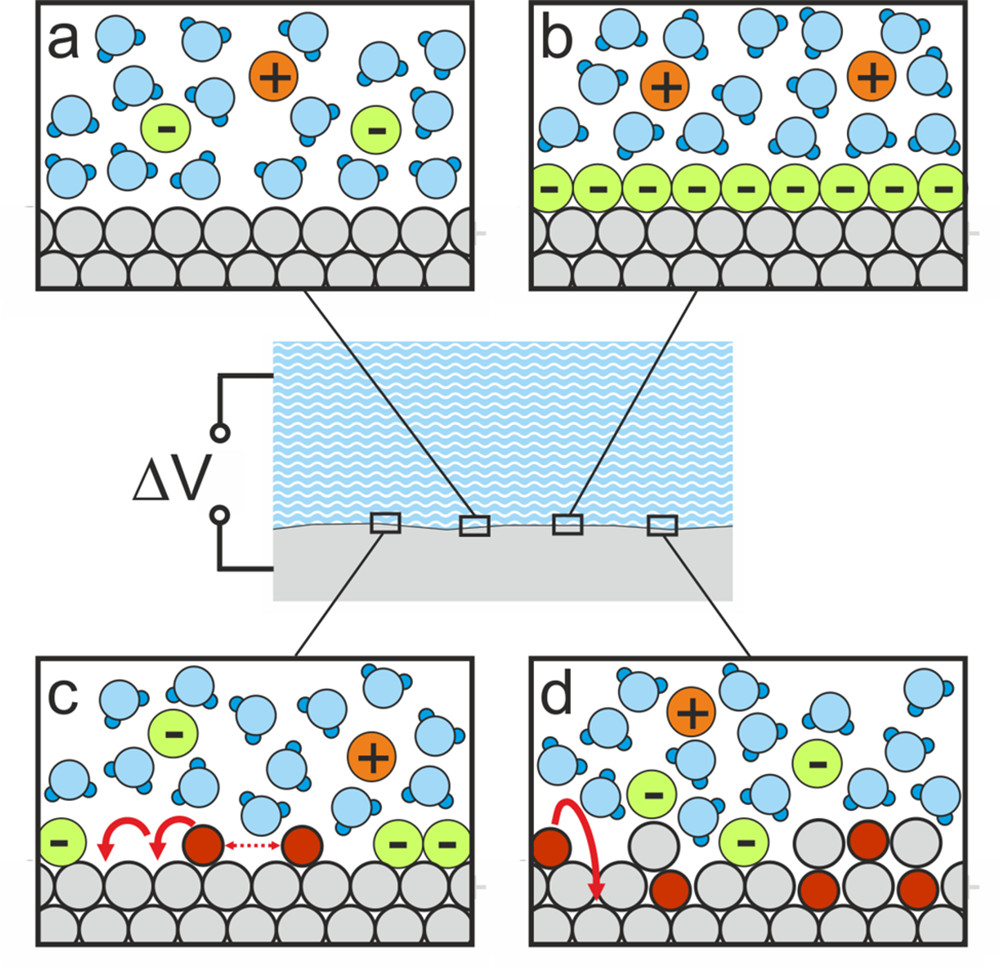
\includegraphics[scale=0.95]{figs/edl_figure.jpeg}
	\legend{Fonte: \citeauthor{edl_article}.}
	\label{fig:edl}
\end{figure}

As alterações estruturais provocadas pela variação do potencial externo é refletida nas propriedades vibracionais do sistema, como observado por meio da espectroscopia de absorção de radiação infravermelho (\textit{surface-enhanced infrared absorption spectroscopy}--SEIRAS) \cite{raman1}, o qual encontrou modificações no modo vibracional de deformação angular e um aumento do número de ligações de hidrogênio indo de potenciais negativo para positivos. Além disso, trabalhos de espectroscopia por Geração de Soma de Frequências (\textit{Sum frequency generation}--SFG), sensível somente à interface água/metal, identificou variações nas frequências mais altas de estiramento devido à variação do potencial e associaram tais modificações à ligações OH livre apontadas para o eletrodo de ouro, além de observarem uma fraca interação dessas moléculas com o metal \cite{sfg1,sfg2,sfg_kramer}. 


Em suma, resultados experimentais observam uma tendência das moléculas de se aproximarem (afastarem) do eletrodo para potenciais positivos (negativos). No entanto, os modelos experimentais ou apresentam resultados controversos sobre a estrutura da água ou são sensíveis a vibrações específicas. Isso posto, simulações computacionais são fundamentais para complementar e auxiliar na interpretação de resultados experimentais, uma vez que permite identificar estruturas cuja sensibilidade dos experimentos não captam \cite{simulacao_vibrational}. Entretanto, a modelagem computacional de processos eletroquímicos possui elevado custo, pois requerem a descrição da superfície carregada e as espécies que compõem o eletrólito e não existe uma abordagem unificada sobre como descrever tais estruturas \cite{electro_curcinotta}.


Nesse sentido, processos eletroquímicos da EDL são modelados explicitamente por meio de simulações de dinâmica molecular \textit{ab initio} ou por meio de modelos de campo médio (modelos contínuos). No primeiro caso todo o sistema é tratado atomisticamente, porém não captura corretamente efeitos eletrostáticos de longo alcance e limita o tamanho do sistema simulado \cite{review_electro}. Por outro lado, modelos contínuos representam o efeito das moléculas de água através de um meio dielétrico e não consideram a forte polarização das moléculas de água que ocorre na superfície do eletrodo \cite{hydrogen4,edl}. Isso significa que para construir modelos mais realísticos dessa interface é necessário compreender as propriedades estruturais e vibracionais da água adsorvida no metal com um potencial externo aplicado, de modo a compreender o comportamento da estrutura eletrônica da água durante o processo eletroquímico \cite{electro_curcinotta,bias_agua1}.


Na simulação eletroquímica é necessário definir o nível de aproximação através do qual os componentes da célula eletroquímica serão descritos, bem como definir o método através do qual a superfície será carregada. Um dos primeiros estudos nessa direção consistiu em simulações empíricas de dinâmica molecular clássica, no qual a eletrização da superfície metálica do eletrodo era alcançada por meio de cargas induzidas nos átomos do eletrodo \cite{charge1}. No âmbito da DFT, Neurock et. al implementou a eletrização de uma superfície metálica por meio da variação de elétrons no eletrodo e a diferença de potencial era introduzida por meio de uma camada de vácuo entre as moléculas da solução e comparado com um potencial de referência artificial (eletrodo de hidrogênio). Com essa abordagem, estudou-se a resposta da polarização da interface água/Pd(111) e água/Cu(111) em relação a um potencial externo \cite{charge2,bias-pd}. Outras implementações nesse sentido surgiram na literatura ao longo dos anos e forneceram detalhes da interface água/metal, bem como os efeitos de polarização, detalhes sobre processos que ocorrem na EDL e informações sobre energias de ativação \cite{hydrogen2,hydrogen1,hydrogen3,hydrogen4,hydrogen5}. \citeauthor{potencial1} propuseram abordar o problema acoplando o sistema a um potenciostato mantido a um potencial fixo e permitindo a troca de elétrons. Em síntese, esses modelos controlam o potencial aplicado a partir da carga adicionada ou subtraída do eletrodo, ao passo que, nos experimentos o que se controla é o potencial aplicado.

Nesse sentido, \citeauthor{artigo-luana} propuseram utilizar o formalismo de Funções de Green Fora do Equilíbrio (\textit{Non--Equilibrium Green’s Function--NEGF}) para investigar processos eletroquímicos. Com isso, os autores observaram o comportamento dependente da molécula de água em relação ao potencial externo aplicado e analisaram como a posição de mínimo é afetada pelo potencial externo. Essa abordagem permite controlar o potencial aplicado aos eletrodos sem alterar a carga total do sistema. Além disso, essa metodologia trata todos os elementos que compõem um sistema eletroquímico ao nível atomístico. Isso permite acompanhar com mais acurácia as interações e trocas de carga que ocorrem na interface entre a água e o metal. 

%Considerando a acurácia da estrutura eletrônica que essa metodologia fornece e as potenciais contribuições acerca das interações da interface água/metal, nesse capítulo abordaremos com mais detalhes esse formalismo. Iniciaremos apresentando os valores esperados de observáveis fora do equilíbrio, Seção \ref{sec:fora}; em seguida apresentaremos o formalismo de Funções de Green Fora do Equilíbrio aplicado a transporte eletrônico e, em seguida, mostraremos como esse formalismo pode ser usado para obter as propriedades eletrônicas e as forças atômicas da interface água/metal à medida que se aplica um potencial externo ao sistema. Por fim, apresentaremos o código computacional \textit{Transiesta} \cite{transiesta1}\cite{transiesta2} responsável por realizar as simulações computacionais.
 

\section{Valores Esperados de Observáveis Fora do Equilíbrio}

De modo geral, o problema de transporte eletrônico envolve um sistema no qual os eletrodos são descritos por diferentes potenciais eletroquímicos acoplados a uma região de espalhamento, o que constitui um sistema fora do equilíbrio. Para tratar problemas desse tipo, consideramos que o hamiltoniano do sistema é composto por um termo não interagente $H_0$ quadrático, um termo que descreve as interações entre partículas $H_i$ e por $H'(t)$ que representa uma pertubação aplicada ao sistema a partir de um tempo $t_0$, ou seja:
\begin{equation}\label{eq:hamiltoniano}
    \ham(t)=H_0+H_i+H'(t)
\end{equation}

Para o problema de transporte eletrônico, essa pertubação tem origem na diferença de potencial dos eletrodos. Considerando que antes da pertubação ser aplicada, o sistema esteja em equilíbrio termodinâmico com um reservatório térmico à temperatura T e um reservatório de partículas descrito por um potencial eletroquímico $\mu$, de modo que a matriz densidade do sistema no ensemble grande canônico é dado por:
\begin{equation}
    \rho(H)=\frac{e^{\beta H}}{\Tr[e^{-\beta H}]}
\end{equation}
onde $H=H_0+H_i$ e a energia das partículas foi medida em relação a $\mu=0$ por simplicidade.

Para calcular o valor esperado de observáveis para tempos $t>t_0$ de acordo com a representação de Heisenberg, tem-se:
\begin{equation}\label{eq:operador}
    \expval{O_{\ham}(t)}=\Tr[\rho(H)O_{\ham}(t)]
\end{equation}

Assim, para calcular a expressão \eqref{eq:operador}, define-se as representações de Schr\"{o}dinger e de Heisenberg de forma que elas coincidam no tempo $t_0$, isso equivale a:
$$
\ket{\Psi_{\ham}}=\ket{\Psi_S(t_0)}\quad\text{e}\quad O_{\ham}(t_0)=O_S   $$
logo, a evolução temporal de $\ham(t)$ é definida por:
\begin{equation}\label{eq:ev1}
    O_{\ham}(t)\equiv u^\dagger_{\ham}(t,t_0)O_S u_{\ham}(t,t_0)
\end{equation}
e o operador de evolução temporal é dado por:
\begin{equation}
    u_{\ham}(t,t_0)=\sum_{n=0}^{\infty}\frac{(-i)^n}{n!\hbar^n}\int_{t_0}^{t}\dd{t_1}\ldots\int_{t_0}^{t}\dd{t_n}\mathrm{T}\Bqty{\ham(t_1)\ldots\ham(t_n)}=\mathrm{T}\Bqty{e^{-\frac{i}{\hbar}\int^t_{t_0}\dd t'\ham(t')}}
\end{equation}
onde $\mathrm{T}$ é o operador de ordenamento temporal, que organiza o produtos dos operadores de acordo com suas ordens temporais, isto é, 
\begin{equation}
  \mathrm{T}\Bqty{A_1(t_1)A_2(t_2)\ldots A_n(t_n)}=(\pm1)^{P}A_{i_1}(t_{i_1})A_{i_2}(t_{i_2})\ldots A_{i_n}(t_{i_n})\;,\quad t_{i_1}>\ldots>t_{i_n}
\end{equation}
onde $P$ é o número de permutações realizadas entre os operadores em relação a ordem original, o sinal positivo corresponde a bósons e o negativo a férmions. Por outro lado, como $H=H_0+H_i$ não possui dependência temporal explícita, então a sua evolução de H é dada por:
\begin{equation}
    O_{H}(t)\equiv u^{\dagger}_H(t,t_0)O_Su_H(t,t_0)\quad\Rightarrow\quad O_S\equiv u_H(t,t_0)O_H(t)u^{\dagger}_{H}(t,t_0)
\end{equation}
onde o operador evolução temporal $u_H(t,t_0)$ é dado por:
\begin{equation}\label{eq:ev2}
    u_H(t,t_0)=e^{-i\frac{H}{\hbar}(t-t_0)}
\end{equation}

Substituindo a Equação \eqref{eq:ev1} na Equação \eqref{eq:ev1}, obtemos:
\begin{equation}\label{eq:observador}
    O_{\ham}(t)=u^{\dagger}_{\ham}(t,t_0)u_{H}(t,t_0)O_{H}(t)u^{\dagger}_H(t,t_0)u_{\ham}(t,t_0)=v^{\dagger}_H(t,t_0)O_H(t)v_H(t,t_0)
\end{equation}
onde $v_H(t,t_0)=u^{\dagger}_H(t,t_0)u_{\ham}(t,t_0)$.

Para obter o valor esperado de um operador fora do equilíbrio é conveniente remover a dependência explícita de $H'(t)$, de modo que a evolução temporal dos operadores seja governada somente por $H=H_0+H_i$. Assim, após algumas manipulações matemáticas \footnote{Os detalhes matemáticos dessas passagens podem ser consultadas em: \citetext{tese-pedro}}, o observável $O_\mathscr{H}(t)$ pode ser reescrito em termos de um operador de ordenamento de contorno $\mathrm{T}_{C_t}$, como está mostrado na Equação \eqref{eq:contorno}. Esse operador organiza o produto dos operadores de acordo com os argumentos de tempo no contorno $C_t $, que inclui os ramos do um contorno sobre o eixo real do tempo $t_0$ até $t$ e de volta a $t_0$
. 
\begin{eqnarray}\label{eq:contorno}
\mathnormal{O}_{\mathscr{H}}(t) &=& v_{\mathnormal{H}}^{\dagger}(t,t_{0})\mathnormal{O}_{\mathnormal{H}}(t)v_{\mathnormal{H}}(t,t_{0})\nonumber\\
&=&\mathrm{T}_{C_{2}}\left\{ e^{-\frac{\imath}{\hbar}\int_{C_{2}}d\tau\mathnormal{H}'_{\mathnormal{H}}(\tau)}\right\}\mathnormal{O}_{\mathnormal{H}}(t)\mathrm{T}_{C_{1}}\left\{ e^{-\frac{\imath}{\hbar}\int_{C_{1}}d\tau\mathnormal{H}'_{\mathnormal{H}}(\tau)}\right\}\nonumber\\
&=&\mathrm{T}_{C_{t}}\left\{ e^{-\frac{\imath}{\hbar}\int_{C_{t}}d\tau\mathnormal{H}'_{\mathnormal{H}}(\tau)}\mathnormal{O}_{\mathnormal{H}}(t)\right\}
\end{eqnarray}

A partir desse processo, a dependência explícita de $H'(t)$ foi removida, de modo que a evolução temporal dos operadores é governada somente por $H=H_0+H_i$. Por meio de um procedimento análogo é possível simplificar a expressão \eqref{eq:contorno} e descrevê-la somente em termos de $H_0$, de modo que a complicação em relação ao termo $H_i$, que descrevem as interações possíveis entre as partículas, é removida.
\begin{equation}
O_{\ham}(t)=\mathrm{T}_{C_t}\Bqty{ e^{-\frac{i}{\hbar}\int_{C_t}\dd\tau H^i_{H_0}(\tau) }e^{-\frac{i}{\hbar}\int_{C_t}\dd\tau H'_{H_0}(\tau)} O_{H_0}(t) }=\mathrm{T}\Bqty{S^i_{C_t}S'_{C_t}O_{H_0}(t)}
\end{equation}
onde $S^i_{C_t}=e^{-\frac{i}{\hbar}\int_{C_t}\dd\tau H^i_{H_0}(\tau) }$ e $S'_{C_t}=e^{-\frac{i}{\hbar}\int_{C_t}\dd\tau H'_{H_0}(\tau)}$.

Assim, após escrever a matriz densidade $\rho(H)$ em termos de $H_0$, o valor esperado de um observável físico fora do equilíbrio na representação de interação é dado por:
\begin{eqnarray}
\expval{\mathnormal{O}_{\mathscr{H}}(t)} &=& \dfrac{\Tr[e^{-\beta\mathnormal{H}}\mathnormal{O}_{\mathscr{H}}(t)]}{\Tr[e^{-\beta\mathnormal{H}}]} = \dfrac{\Tr[e^{-\beta\mathnormal{H}_{0}}\nu(t_{0}-\imath\hbar\beta,t_{0})\mathnormal{O}_{\mathscr{H}}(t)]}{\Tr[e^{-\beta\mathnormal{H}_{0}}\nu(t_{0}-\imath\hbar\beta,t_{0})]}\nonumber\nonumber\\
&=& \dfrac{\expval{\nu(t_{0}-\imath\hbar\beta,t_{0})\mathnormal{O}_{\mathscr{H}}(t)}_{0}}{\expval{\nu(t_{0}-\imath\hbar\beta,t_{0})}_{0}}\nonumber\\
&=& \dfrac{\expval{\mathnormal{T}_{\tilde{C}}\left\{\mathnormal{S}'_{C}\mathnormal{S}_{\tilde{C}}^{\imath}\mathnormal{O}_{\mathscr{H}}(t)\right\}}_{0}}{\expval{\mathnormal{T}_{\tilde{C}}\left\{ \mathnormal{S}'_{C}\mathnormal{S}_{\tilde{C}}^{\imath}\right\}}_{0}}
\end{eqnarray}
onde $\tilde{C}$ representa o caminho da Figura \ref{fig:contorno} e $\expval{\quad}_0$ indica que o valor esperado é calculado com respeito a $\rho(H_0)$. Esse procedimento faz com que o valor esperado dependa da matriz densidade $\rho(H_0)$ quadrática e possibilita descrever o problema fora do equilíbrio de forma diagramática. \cite{tese-pedro}
\begin{figure}[H]
	\centering
	\includegraphics[scale=0.65]{figs/contorno2.PNG}
	\caption{\textit{Contorno $\tilde{C}$ composto pelos contornos C sobre o eixo real e $C_\nu$ perpendicular ao eixo real. Fonte: \citeauthor{tese-pedro}.}}
	\label{fig:contorno}
\end{figure}  

\section{Funções de Green Fora do Equilíbrio\label{sec:fora}}

As funções de Green são definidas como as soluções de equações diferenciais inomogêneas, cuja expressão é dada por:
$$
    \bqty{z-L(\vb{r})}\green=\delta(\vb{r}-\vb{r'})
$$
sujeito à condições de contorno situadas na superfície $S$ do domínio $\Omega$ de $\vb{r}$ e $\vb{r'}$. De acordo com a notação utilizada, $z$ é uma variável complexa com $\lambda\equiv Re\Bqty{z}$ e $s\equiv Im\Bqty{z}$ e $L(\vb{r})$ é um operador diferencial linear, hermitiano e que possui um conjunto de autofunções $\Bqty{\varphi_n(\vb{r})}$ que satisfazem as mesmas condições de contorno que $\green$ \cite{green}. Para obter as propriedades das Funções de Green, é mais conveniente reescrever a equação acima utilizando a notação de Dirac:
\begin{eqnarray}\label{eq:dirac}
    \pqty{z-L}G(z)&=&\mathbb{1}\delta(z)\qquad\text{onde,}\\
    \quad\green&\equiv&\mel{\vb{r}}{G(z)}{\vb{r'}}\nonumber
\end{eqnarray}

Fora do equilíbrio, a função de Green é definida ordenada no contorno C (Figura \ref{fig:contorno}), que  se inicia em $t_0$, continua pelo eixo real, passa uma vez em $t_1$ e em $t_{1'}$ para por fim  retornar para $t_0$ e é dada pela equação:
\begin{equation}
    G(1,1')\equiv -\frac{i}{\hbar}\expval{ T_C\Bqty{ \Psi_\ham(1)\Psi^{\dagger}_\ham(1') } }
\end{equation}

onde $(1)\equiv(\vb{r}_1,\sigma_1,t_1)$ e $\Psi_\mathscr{H}$ mostra a dependência da função de onda em termos do Hamiltoniano definido na Equação \eqref{eq:hamiltoniano}. A representação de interação da Função de Green Fora do Equilíbrio é obtida de forma análoga à seção anterior, onde as grandezas envolvidas foram escritas com a dependência de $H_0$:
\begin{equation}
    G(1,1')=-\frac{i}{\hbar}\frac{\expval{T_C\Bqty{S'_CS^i_C\Psi_{H_0}(1)\Psi^{\dagger}_{H_0}(1')}  }_0 }{\expval{T_C\Bqty{S'_cS^{i}_C} }_0}
\end{equation}

\end{comment}
\section{Definindo o Problema\label{sec:problema}}

O formalismo de funções de Green fora do equilíbrio é comumente utilizado para tratar problemas de transporte eletrônico na escala atômica, no qual um objeto nanométrico situado na região central é conectado a dois reservatórios \textit{bulk} que atuam como eletrodos. Nesse arranjo, o potencial externo é aplicado por meio da diferença entre os potenciais químicos dos reservatórios. De forma análoga, uma célula eletroquímica é composta por dois eletrodos metálicos separados por uma solução eletrolítica majoritariamente composta por água. Além disso, ao aplicar uma diferença de potencial em uma célula eletroquímica o sistema fica fora do equilíbrio. Essas semelhanças permitem utilizar a abordagem de NEGF no contexto da eletroquímica para investigar atomisticamente as propriedades eletrônicas e o comportamento da molécula de água na interface com o eletrodo a diferentes potenciais como reportado por \citeauthor{artigo-luana}. 
\begin{figure}[t!]
	\centering
	\caption{Ilustração do sistema utilizado para aplicar um potencial externo sobre a interface água/metal e as regiões correspondentes aos eletrodos e região de espalhamento.}
	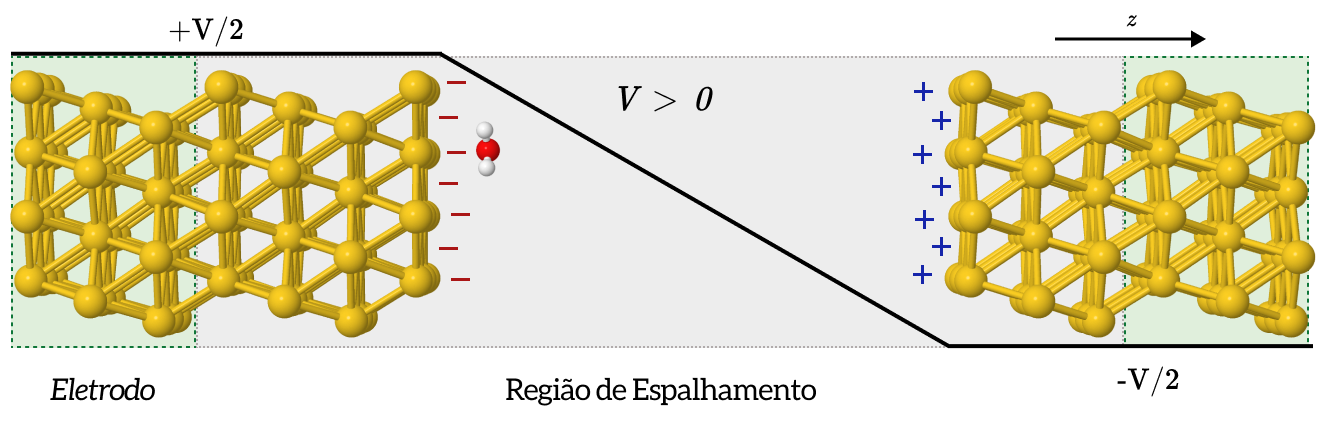
\includegraphics[scale=0.33]{figs/sistema_negf.png}
	\legend{Fonte: compilação da autora}
	\label{fig:celula}
\end{figure}

A adaptação do formalismo de NEGF a uma célula eletroquímica constitui em associar os componentes típicos da abordagem de transporte às regiões da célula eletroquímica. Assim, os reservatórios de carga correspondem aos eletrodos da célula eletroquímica e a região de espalhamento inclui algumas camadas do eletrodo metálico e a região central da célula eletroquímica, como está esquematizado na Figura \ref{fig:celula}. O sistema representado nessa imagem ilustra o protótipo de uma célula eletroquímica utilizado para investigar nesse trabalho a interface água/metal sob um potencial externo. Nessa imagem, os eletrodos são separados por uma região de vácuo e a região central da célula eletroquímica é composta por uma estrutura de água adsorvida no eletrodo esquerdo. Além disso, nessa configuração não existe fluxo de corrente pois a barreira de energia ($ \sim8 $ eV) da água é larga o suficiente para garantir que não haja fluxo, ainda que o formalismo de transporte seja capaz de tratar sistemas que tenham fluxo de corrente na região de espalhamento. Assim, esse sistema funciona como um modelo do comportamento das moléculas de água na interface sob um potencial externo aplicado e consequentemente, permite entender modelar uma  melhor os processos que ocorrem na numa célula eletroquímica.




%Do ponto de vista eletrostático, o potencial externo aplicado sobre os eletrodos produz um deslocamento de energia no espectro, ao passo que na região estendida surgirá um potencial não trivial que deve ser calculado por auto-consistência, de modo que as condições de contorno coincidam com as dos eletrodos- Figura \ref{fig:abordagem}(b). \cite{tese-alexandre}

No âmbito do formalismo de NEGF, o hamiltoniano total que descreve o sistema pode ser dividido em três partes: $H_C$ que descreve os eletrodos direito (R) e esquerdo (L), $H_T$ que representa o acoplamento entre a região central e os contatos e $H_M$ que descreve a região central onde ocorrem as interações. Tais contribuições podem ser descritos como segue abaixo:
\begin{eqnarray}
	\ham&=&(H_C^L+H_C^R)+(H_T^L+H_T^R)+H_M \\    
	H^{\alpha}_C&=&\sum_n E_{n\alpha} d^{\dagger}_{n\alpha} d_{n\alpha} \\
	H^{\alpha}_T&=&\sum_{n,k}\pqty{V_{n\alpha,k} d^{\dagger}_{n\alpha}c_k+h.c}\\
	H_M&=&H_M\pqty{\{ c^{\dagger}_k\};\{c_k\}}
\end{eqnarray}
onde $d^{\dagger}_{n\alpha}$ e $d_{n\alpha}$ são operadores de criação e destruição de um elétron no eletrodo $\alpha$ no estado n, respectivamente; ao passo que os operador $c^{\dagger}_k$/$c_k$ criam/destroem um elétron no estado k da região de interação. Os elétrons do contato são considerados não interagentes, pois os eletrodos são metálicos e estão em equilíbrio termodinâmico. Os potenciais $V_{n\alpha,k}$ dependem das densidades de cargas que são determinadas por cálculos auto consistentes. A forma do hamiltoniano $H_M$ depende do tipo de sistema que vai ser analisado.

Ao aplicar uma diferença de potencial, ocorre uma redistribuição de carga, logo é conveniente descrever o hamiltoniano em termos da densidade eletrônica. Assim, podemos descrever o sistema como uma matriz hamiltoniana e uma matriz de \textit{overlap}. Para construir os hamiltonianos dos eletrodos, consideramos que cada célula unitária que os compõem interagem somente com os primeiros vizinhos, de modo que as matrizes do hamiltonianos dos eletrodos são dadas por:
\begin{equation}
	\mathcal{H}_L =\begin{pmatrix}
		\ddots  & \vdots  & \vdots & \vdots & \vdots \\
		\ldots & H_L^0 & H_L^1 & 0 &0  \\
		\ldots & H_L^{1\dagger} & H_L^0 & H_L^1 & 0 \\
		\ldots & 0 & H_L^{1\dagger} & H_L^0 & H_L^1 \\
		\ldots & 0 & 0 & H_L^{1\dagger} & H_L^0 \\
	\end{pmatrix}\qquad 
	\mathcal{H}_R= \begin{pmatrix}
		H_R^0  & H_R^1   & 0 & 0& \ldots \\
		H_R^{1\dagger} & H_R^0 & H_R^1 & 0 &\ldots  \\
		0 & H_R^{1\dagger} & H_R^0 & H_R^1 & \ldots \\
		0 & 0 & H_R^{1\dagger} & H_R^0 & \ldots\\
		\vdots & \vdots & \vdots & \vdots & \ddots \\
	\end{pmatrix}
\end{equation}
onde o índice 0 representa a célula unitária e o índice 1 representa o acoplamento entre as células adjacentes; os subíndices R e L correspondem aos eletrodos esquerdos e direitos, respectivamente.


Para construir o hamiltoniano da região de espalhamento, adiciona-se à essa região algumas células unitárias dos eletrodos, a fim de garantir que a queda na diferença de potencial ocorra somente na parte central, de modo que a estrutura eletrônica dos eletrodos não seja alterada. Assim o hamiltoniano $\mathcal{H}$ do sistema completo é dado por:
\begin{equation}\label{eq:matriz}
\mathcal{H}=\begin{pmatrix}
\ddots & \vdots  & \vdots & \vdots & \vdots & \vdots & \iddots \\
\ldots  & H_L^0 & H_L^1 & 0 & 0 & 0 & \ldots \\
\ldots & H_L^{1\dagger} & H_L^0 & H_{LM} & 0 & 0 & \ldots \\
\ldots & 0 & H_{ML} & H_{M} & H_{MR} & 0 &\ldots  \\
\ldots & 0 &0  & H_{RM} & H_R^1 & H^1_R &\ldots  \\
\ldots & 0 & 0 & 0 & H_L^{1\dagger} & H_R^0 &\ldots \\
\iddots& \vdots & \vdots & \vdots & \vdots & \vdots & \ddots \\
\end{pmatrix}
\end{equation}
onde $H_{LM}$ e $H_{RM}$ representam o acoplamento dos eletrodos esquerdo e direito com a região de espalhamento, respectivamente. Essa matriz é infinita e não periódica.

Assim, para uma dada energia $\varepsilon$, o problema pode ser escrito em termos da função de Green retardada:
\begin{equation}
    \pqty{\varepsilon\mathcal{S}-\mathcal{H}}G^r(\varepsilon)=\mathbb{1}
\end{equation}
com $\mathcal{S}$ a matriz de overlap que segue a mesma convenção dos elementos de $\mathcal{H}$\footnote{A convenção adotada é a de que as letras caligráficas $\mathcal{H}$ e $\mathcal{S}$ representam matrizes infinitas e $H$ e $S$ matrizes finitas}. A expressão acima pode ser reescrita em termos dos hamiltonianos dos eletrodos da seguinte forma:
\begin{equation}\label{eq:matriz-esparsa}
    \begin{pmatrix}
\varepsilon\mathcal{S}_{L}-\mathcal{H}_{L} & \varepsilon\mathcal{S}_{LM}-\mathcal{H}_{LM} &0  \\
 \varepsilon\mathcal{S}_{ML}-\mathcal{H}_{ML}&\varepsilon S_{M}-H_{M}  &\varepsilon\mathcal{S}_{ML}-\mathcal{H}_{ML}  \\
0& \varepsilon\mathcal{S}_{RM}-\mathcal{H}_{RM} & \varepsilon\mathcal{S}_{R}-\mathcal{H}_{R} \\
\end{pmatrix}\begin{pmatrix}
G^r_{L} & G^r_{LM} &G^r_{LR}  \\
G^r_{ML} &G^r_{M}  & G^r_{MR} \\
G^r_{RL} &G^r_{RM}  &G^r_{R} \\
\end{pmatrix}=\mathbb{1}
\end{equation}

Como foram introduzidas no hamiltoniano da região de espalhamento algumas células unitárias dos eletrodos, essa região sentirá o efeito da interação com os eletrodos da mesma forma se tivéssemos considerando o sistema completo e com a vantagem de lidar com matrizes de dimensões finitas.

Assim, a partir da Equação \eqref{eq:matriz} podemos obter a função de Green correspondente à região de espalhamento:
\begin{equation}\label{eq:green}
    G_M^r=\pqty{\varepsilon S_M-H_M-\Sigma^{r}_L-\Sigma^{r}_R}^{-1}
\end{equation}
onde $\Sigma^{r}_L$ e $\Sigma^{r}_L$ são as autoenergias dos eletrodos esquerdo e direito, respectivamente, e são dadas por:
\begin{eqnarray}\label{eq:auto1}
\Sigma^{r}_L&=&\pqty{\varepsilon \mathcal{S}_{ML}-\mathcal{H}_{ML}}\pqty{\varepsilon \mathcal{S}_{L}-\mathcal{H}_{L}}^{-1}\pqty{\varepsilon \mathcal{S}_{LM}-\mathcal{H}_{LM}}\\\label{eq:auto2}
\Sigma^{r}_R&=&\pqty{\varepsilon \mathcal{S}_{MR}-\mathcal{H}_{MR}}\pqty{\varepsilon \mathcal{S}_{R}-\mathcal{H}_{R}}^{-1}\pqty{\varepsilon \mathcal{S}_{RM}-\mathcal{H}_{RM}}
\end{eqnarray}

Assim, o desafio passa a ser o cálculo das autoenergias dos eletrodos, pois esses envolvem a manipulação de matrizes de dimensões infinitas. No entanto, os acoplamentos dos eletrodos à região de espalhamento ($H_{LM}$ e $H_{RM}$) possuem como termos não nulos o bloco adjacente a esta região, cujas dimensões são da ordem da célula unitária do eletrodo. Esses elementos são obtidos por métodos semianalíticos ou por métodos recursivos \cite{smeagol1,smeagol2}. 

Até aqui obtemos o função de Green de um sistema aberto fora do equilíbrio, onde \textit{a priori} os hamiltonianos do sistema eram conhecidos. Por outro lado, o caso em que a dependência funcional do hamiltoniano com a densidade de carga $n(\vb{r})$ é conhecida constitui o caso mais comum em DFT, ou seja $\mathcal{H}=\mathcal{H}\bqty{n}$. Isso ocorre pois essa dependência é obtida por meio de cálculos padrões de estrutura eletrônica, onde não se tem potencial externo. Assim, na situação de equilíbrio e sem potencial aplicado, os eletrodos são tratados como reservatórios de carga, cujo potencial químico é $\mu_0$ dado pelo cálculo de bulk do metal.

Ao aplicar o potencial externo $V$  sobre o sistema, ocorrem mudanças na polarização e na carga superficial da região de espalhamento. Essas mudanças alteram apenas a parte de espalhamento, de modo que a densidade de carga e os termos do hamiltoniano do eletrodo não são modificados. Assim,  o efeito do potencial externo é um \textit{shift} na energia e o hamiltoniano do sistema completo é dado por:
\begin{equation}
    \mathcal{H}=\begin{pmatrix}
\mathcal{H}_L+\mathcal{S}_L\;\frac{eV}{2} & \mathcal{H}_{LM} &0  \\
\mathcal{H}_{ML} & H_M & \mathcal{H}_{MR} \\
0 & \mathcal{H}_{RM} & \mathcal{H}_R-\mathcal{S}_R\frac{eV}{2} \\
\end{pmatrix}
\end{equation}

Onde nesse caso, $H_M=H_M\bqty{n}$ corresponde à Hamiltoniana de Kohn-Sham e a Função de Green que descreve a região de espalhamento do sistema fora do equilíbrio continua sendo a Equação \eqref{eq:green}. Os demais observáveis do sistema são calculados por recorrência, e em particular a matriz densidade é obtida por:
\begin{equation}\label{eq:matriz-densidade}
    D_{\mu\nu}=\int_{-\infty}^{\infty}\dd{E}\bqty{\rho_{\nu\nu}^L f(E-\mu_L)+\rho_{\mu\nu}^Rf(E-\mu_r)}
\end{equation}
onde os índices $\mu$ e $\nu$ correspondem ao estados eletrônicos da região de espalhamento, $\mu_L$ e $\mu_r$ são os potenciais eletroquímicos dos eletrodos que definem o potencial externo $V=\mu_l-\mu_R$ e são definidos por: $\mu_{L/R}=\mu_0\pm V/2$; $f(E)$ é função de Fermi para uma dada temperatura T:$$f(E)=\frac{1}{1+e^{E/kT}}$$
Por fim, $\rho^{L/R}$ são as matrizes de densidade espectral correspondente aos eletrodos:
\begin{eqnarray}
    \rho^{L/R}&=&G(E)\Gamma_{L/R}(E)G^{\dagger}(E)\\
    \text{onde,}\qquad\Gamma_{L/R}&=&\frac{i}{\pi}\bqty{\Sigma_{L/R}(E)-\Sigma^{\dagger}_{L/R}(E)}
\end{eqnarray}

O efeito do potencial externo aplicado ao sistema é introduzido a partir das diferenças entre as estruturas eletrônicas dos eletrodos, isto é, a partir da diferença entre os respectivos potenciais químicos $  \mu_L$ e $ \mu_R  $ \cite{negf}. Assim, no equilíbrio (V=0) tem-se que funções de distribuição de Fermi dos dois eletrodos são iguais $ \mu_L=\mu_R $, de modo que as autofunções podem ser reescritas por:
\begin{equation}
	\Sigma=-\frac{1}{2}\bqty{G^{-1}-\epsilon S_M+H_M}
\end{equation}

Então, no equilíbrio:
\begin{eqnarray}
	G(E)\Gamma(E)G^{\dagger}(E)&=&i G\bqty{\Sigma-\Sigma^{\dagger}}G^{\dagger}\nonumber \\
	&=&\frac{i}{2}G\bqty{(G)^{-1}-(G^{\dagger})^{-1}}G^{\dagger}\nonumber\\
	&=&-\Im{G}
\end{eqnarray}

Isso permite reescrever a matriz densidade $ D_{\mu\nu} $ como uma soma da contribuição no equilíbrio e fora $ D_{\mu\nu}=D_{eq}+D_{neq} $, onde:
\begin{equation}\label{eq:eq}
	D_{eq}=-\frac{1}{\pi}\int\dd{E}\Im{G(E)}f(E-\mu)
\end{equation}
\begin{equation}\label{eq:neq}
	D_{neq}=-\frac{1}{2\pi}\int\dd{E} G(E)\Gamma_R G(E)^{\dagger}\bqty{f(E-\mu_R)-f(E-\mu_L)}
\end{equation}

A integral na parte fora do equilíbrio é limitada pela subtração das funções de Fermi dos eletrodos $ f(E-\mu_L) $ e $ f(E-\mu_R) $ e pode ser calculada no eixo real, ao passo que a matriz no equilíbrio é resolvida por meio do Teorema dos Resíduos no plano complexo. Isso é feito, pois, a função de Green possui polos no eixo de energia real e se comporta de forma irregular. Assim, se torna mais conveniente resolver a integral no plano complexo onde a função de Green é analítica e suave, além de que para resolver a integral basta escolher um contorno que compreenda os polos da função de Fermi\footnote{Os polos $z_j$ da função de Fermi são dados por: $ e^{\frac{z_j-\mu_L}{k_BT}} =-1\Rightarrow z_j=\mu_L+i(2j+1)\pi k_BT$} $z_j=\mu_L+i(2j+1)\pi k_BT$ \cite{tese-pedro}.

Na Figura \ref{fig:contour} estão ilustrados os contornos utilizados para calcular a integral, onde tem-se um contorno sobre o eixo real e outros dois contornos matematicamente equivalentes: circular (linha vermelha) e quadrado (linha azul). O contorno no plano complexo superior é usado para calcular G(E) e no plano inferior para calcular $ G^{\dagger} $; esses contornos são limitados no lado esquerdo pela menor energia do estado ocupado. Após definir os contornos, essas integrais são resolvidas por métodos de quadraturas\footnote{Exemplos de métodos de quadratura: Newton-Cotes, polinômios de Legendre, Gauss-Fermi e Tanh-Sinh.} que dependem de parâmetros tais como o número de polos ($ z_i $) e pontos nos respectivos contornos. Numericamente, a parte fora do equilíbrio é mais cara de se calcular devido ao produto de matriz triplo $ G(E)\Gamma_R G(E)^{\dagger} $ e que pode ser resolvido pelos algoritmos de inversão de matriz \footnote{Exemplos de algoritmos de inversão de matriz: LAPCK, MUMPS ou \textit{Block-tri-diagonal (BTD)}.}. \cite{transiesta2} 

\begin{figure}[h!]
	\centering
	\caption{Contornos utilizados para matriz densidade no equilíbrio nos planos complexos superior (a) e inferior (b). A linha preta representa o contorno sobre o eixo real $ \mathcal{R} $, a linha azul o contorno quadrado $ \mathcal{S} $ e vermelho o circular $ \mathcal{L}$ e $\mathcal{C} $.}
	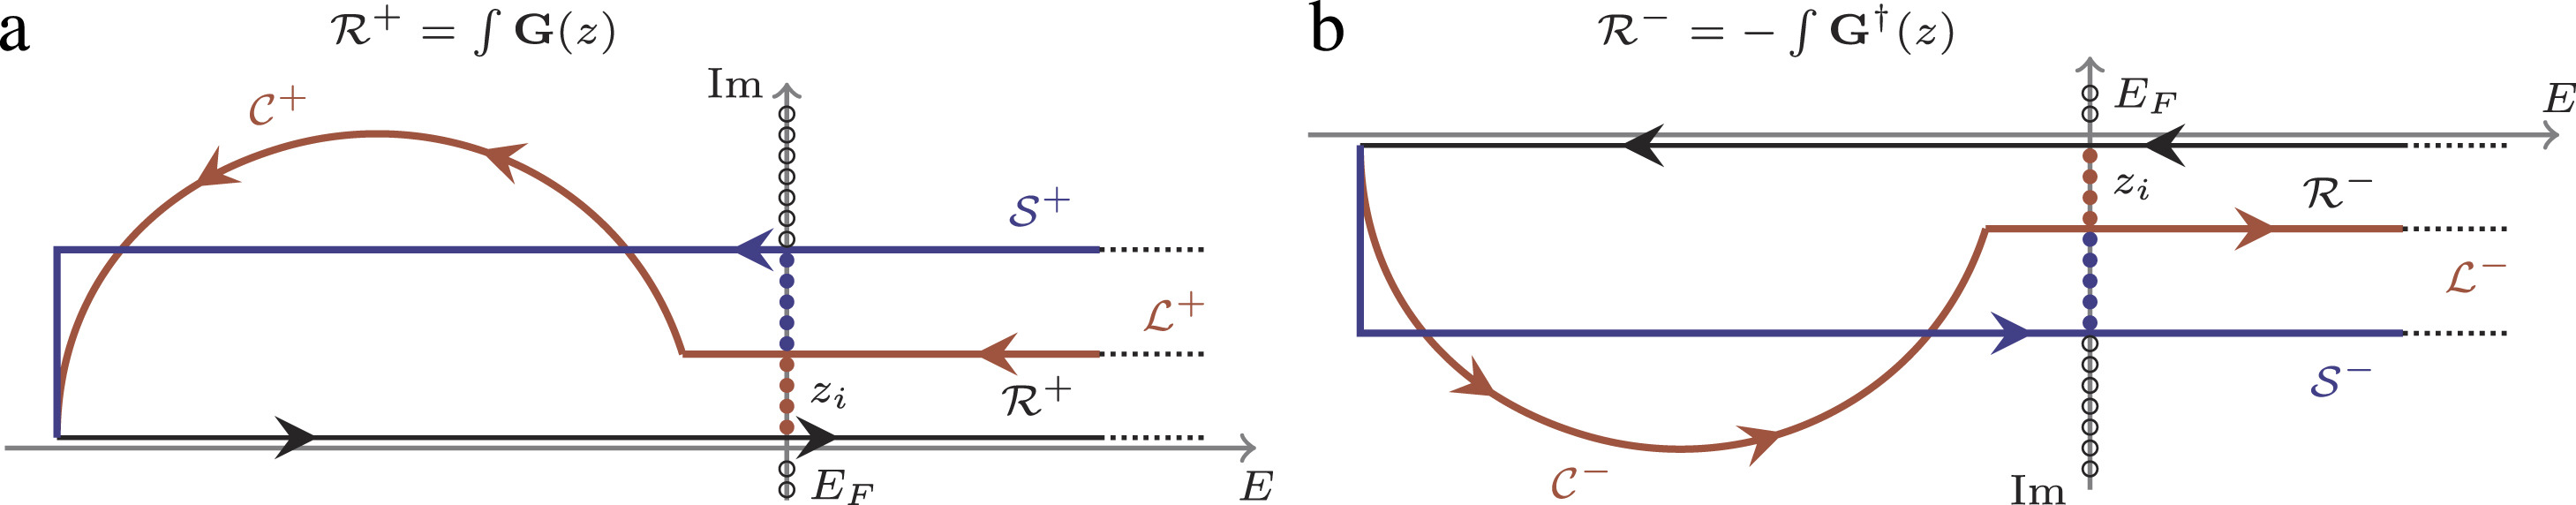
\includegraphics[scale=1]{figs/contour_green.jpg}
	 \legend{Fonte: \citeauthor{transiesta2}.}
	\label{fig:contour}
\end{figure} 

Por fim, o formalismo de NEGF+DFT pode ser encontrado no código \textit{Siesta} através da implementação do \textit{Transiesta}\cite{transiesta1,transiesta2,transiesta3}. A primeira versão do Transiesta foi publicada em \citeyear{transiesta1} e atualmente tem se destacado pela eficiência computacional e acurácia da estrutura eletrônica. Além disso, apresenta flexibilidade de simular situações mais realísticas, tais como a inclusão de defeitos em transporte eletrônico, a possibilidade de usar N>1 eletrodos e o cálculo de forças atômicas fora do equilíbrio \cite{transiesta4}. Em particular, o cálculo de forças permite realizar a otimização das coordenadas a fim de definir a posição de mínimo de acordo com o potencial externo aplicado. Assim, na seção seguinte apresentaremos como fazer o cálculo de forças em problemas fora do equilíbrio.


\subsection{Cálculo de Força Fora do Equilíbrio}
No estado fundamental e em sistemas independente do tempo, as forças que agem no núcleo de moléculas e sólidos podem ser obtidas pelo Teorema de Hellmann-Feynman (HF) \cite{forca-teo}\cite{forca-teo2}. Esse teorema estabelece que, dado uma hamiltoniana dependente de um parâmetro $ \lambda $ e sendo $ \Psi $ quadrado integrável, então, a força generalizada equivale à derivada da energia total em relação ao parâmetro $ \lambda $ (Equação \ref{eq:forca}). Esse teorema é válido tanto para funções de onda exatas ou expandidas em uma base finita.

\begin{equation}\label{eq:forca}
\vb{F}=-\dv{E}{\lambda}=-\underbrace{\flatfrac{\ev**{\pdv{H}{\lambda}}{\Psi}}{\braket{\Psi}{\Psi}}}_{\substack{\text{Força HF}}}-\underbrace{\flatfrac{\bqty{\mel**{\Psi}{H-E}{\pdv{\Psi}{\lambda}}-\mel**{\pdv{\Psi}{\lambda}}{H-E}{\Psi}}}{\braket{\Psi}{\Psi}}}_{\substack{\text{Força de Pulay}}}
\end{equation}

Onde, para $ \Psi $ exato\footnote{A forma convencional do teorema de HF é válido para funções de onda exatas ou expandidas em uma base finita, desde que: (a) as funções de base não dependam de $ \lambda $ ou (b) a derivada da base em relação à $ \lambda $ também faça parte da base. Essas regras são conhecidas por \textit{Condições de Hurley}.} a expressão se reduz à Força de HF e para uma base finita é acrescentado a correção de \textit{Pulay}. Para sistemas dependentes do tempo, $ \Phi=\Phi(t,\vb{r}) $, \citeauthor{force-teo3} propuseram uma definição mais geral do teorema de HF:
\begin{eqnarray}\label{eq:hf-geral}
\vb{F}=-i\hbar\dv{t}\ev**{\pdv{}{\lambda}}{\Phi}&=&-\flatfrac{\ev**{\pdv{H}{\lambda}}{\Phi}}{\braket{\Psi}{\Psi}}\nonumber\\&-&\flatfrac{\bqty{\mel**{\pdv{\Phi}{\lambda}}{H-i\pdv{t}}{\Phi}+\mel**{\Phi}{H+i\pdv{t}}{\pdv{\Phi}{\lambda}}}}{\braket{\Psi}{\Psi}}
\end{eqnarray}

Essa formulação é mais geral e vale para problemas de mecânica quântica fora do equilíbrio com estados estacionários, onde $ \ket{\Phi}=e^{-iEt/\hbar}\ket{\Psi} $. Assim, considerando o parâmetro $ \lambda=\vb{R_I} $  como a posição atômica do núcleo, então a Equação \eqref{eq:hf-geral} se reduz a:
\begin{equation}\label{eq:geral-red}
	\vb{F}_I=-\pdv{\ev{H}{\Psi}}{\vb{R}_I}
\end{equation}

Considerando que na DFT, o estado fundamental de energia é bem definido, de modo que as forças podem ser calculadas como a derivada da energia total com respeito à posição atômica $ \vb{R_I} $. Além disso, a força pode ser separada em duas contribuições:
\begin{equation}\label{eq:force-dft}
	\vb{F}=\vb{F}_{BS}+\vb{F}_{C}
\end{equation}
onde $ \vb{F}_{BS}=-\pdv{E_{BS}}{\vb{R_I}} $ corresponde à contribuição das energias das estruturas de banda e $ \vb{F}_{C} $ inclui as demais contribuições. Assim, considerando a equação de Kohn-Sham (Eq. \eqref{eq:kohn-sham}), o termo $ \vb{F}_{BS} $ equivale a:
\begin{equation}
	\vb{F}^{BS}=-\sum_{\mu\nu}D_{\mu\nu}\pdv{H_{\mu\nu}}{\vb{R}}+\Omega_{\mu\nu}\pdv{S_{\mu\nu}}{\vb{R}}
\end{equation}

onde $D_{\mu\nu}$ é a matriz densidade no equilíbrio e obtida por auto consistência e $\Omega_{\mu\nu}$ é a matriz densidade de energia:
$$\Omega_{\mu\nu}=\sum_i E_i f(E_i)\Psi_{i\mu}\Psi_{i\nu}$$

Como a Equação \eqref{eq:geral-red} é equivalente à \eqref{eq:forca}, e a partir dela a expressão \eqref{eq:force-dft} é obtida, logo ela também é válida para o caso de trasporte eletrônico com estado estacionário. Portanto, os termos $ D_{\mu\nu} $ e $ \Sigma_{\mu\nu} $ podem ser substituídos pelos equivalentes fora do equilíbrio, permitindo assim, calcular as forças atômicas no âmbito do formalismo NEGF+DFT. \cite{force-teo4}


\begin{comment}
\subsection{O código \textit{Transiesta}}
\todo[inline,color=green!40]{Falta mexer nessa parte}
O código Transiesta foi criado em 2002 por meio da implementação do formalismo de NEGF junto com DFT no código \textit{Siesta} pelos autores \citeauthor{transiesta1}. Atualmente, tem se destacado pela eficiência computacional, acurácia da estrutura eletrônica e flexibilidade de simular situações experimentais realísticas, tais como a inclusão de defeitos em transporte eletrônico e a possibilidade de usar N>1 eletrodos. Essas e outras melhorias constituíram o cerne das recentes modificações que o tem colocado em posição de destaque em simulações computacionais de transporte eletrônico \cite{transiesta2}\cite{transiesta3}\cite{transiesta4}. Em particular, a eficiência computacional está relacionado aos algoritmos de inversão utilizados para resolver o produto de matriz triplo. Assim, nessa seção será apresentado o principal algoritmo de inversão utilizado no Transiesta \textit{Block-tri-diagonal}(BTD). 

A utilização de bases atômicas localizadas faz com que as matrizes Hamiltoniana, de densidade e de \textit{overlap} sejam esparsas. Para calcular as funções de Green na situação fora do equilíbrio, é necessário obter a matriz inversa dessas matrizes tridiagonais (incluindo as autoenergias) por meio de algoritmos especializados em inversão com elementos não nulos concentrados em certas posições. Na Figura \ref{fig:matriz}, vemos uma representação ilustrativa dos blocos de matrizes (Eq. \eqref{eq:matriz-esparsa}) que descrevem os eletrodos e a região de espalhamento da abordagem típica de um problema de transporte eletrônico \cite{exemplo}, onde os blocos maiores representam os eletrodos e os menores a região de espalhamento.

\begin{figure}[h!]
	\centering
	\includegraphics[scale=0.3]{figs/matriz_esquema.png}
	\caption{\textit{Esquema ilustrativo das matrizes tridiagonais que descreve um sistema de transporte eletrônico. Fonte: \citeauthor{exemplo}.}}
	\label{fig:matriz}
\end{figure}  

De acordo com esse algoritmo, dado uma matriz tridiagonal $ \vb{M} $, no qual as matrizes que compõem a diagonal ($ \vb{A_1} $ a $ \vb{A_N} $) são quadradas e invertíveis \cite{algoritmo}.

\begin{equation}
	M=\begin{bmatrix}
		\vb{A_1} & \vb{C_2} & 0 & \cdots  & 0 \\ 
		\vb{B_1} & \vb{A_2} & \vb{C_3} & \cdots  & 0\\ 
		0 & \vb{B_2} & \vb{A_3} & \cdots  &0 \\ 
		\vdots  & \vdots  & \vdots  & \vdots  & \vdots \\ 
		0& 0 &0  & 0 & \vb{A_N}
	\end{bmatrix}
\end{equation}
então, os blocos diagonais de $ \vb{M}^{-1} $ são dados por:
\begin{equation}
	(\vb{M}^{-1})_{n,n}=\bqty{\vb{A}_n-\vb{X}_n-\vb{Y}_n}^{-1}
\end{equation}
onde, 
\begin{equation}\label{eq:btd1}
	\vb{X_N}=\left\{\begin{matrix}
		0 & \text{se}\quad n=N\\ 
		\vb{C_{n+1}}\bqty{\vb{A}_{n+1}-\vb{X}_{n+1}}^{-1}\vb{B}_n &\text{se}\quad1\leq m< N 
	\end{matrix}\right.
\end{equation}

\begin{equation}\label{eq:btd2}
	\vb{Y_N}=\left\{\begin{matrix}
		0 & \text{se}\quad n=1\\ 
		\vb{B}_{n-1}\bqty{\vb{A}_{n-1}-\vb{Y}_{n-1}}^{-1}\vb{C}_n &\text{se}\quad1\leq m< N 
	\end{matrix}\right.
\end{equation}

Os termos fora da diagonal são dados por:

\begin{equation}
	(\vb{M}^{-1})_{m,n}=\left\{\begin{matrix}
		-\bqty{\vb{A}_m-\vb{X}_m}^{-1}\vb{B}_{m-1}(\vb{M}^{-1})_{m-1,n} & \text{se}\quad m>n\\ 
		-\bqty{\vb{A}_m-\vb{X}_m}^{-1}\vb{C}_{m-1}(\vb{M}^{-1})_{m+1,n} & \text{se}\quad m<n
	\end{matrix}\right.
\end{equation}
 
Associando esse método ao cálculo das funções de Green fora do equilíbrio, podemos equiparar a matriz $ \vb{G}^{-1} $ à matriz $ \vb{M}^{-1} $, onde as matrizes $ \vb{A}_i,\vb{B}_i $ e $ \vb{C}_i $ correspondem aos elementos não nulos de $ \epsilon\vb{S}-\vb{H}-\vb{\Sigma}_L-\vb{\Sigma}_R $. Na Figura \ref{fig:btd} está ilustrado como os termos que compões a inversa da matriz são obtidos recursivamente. Além disso, vemos que o termo $ \vb{Y}_1 $ resulta na autoenergia do eletrodo esquerdo ($ \Sigma_1 $) e $ \vb{X}_1 $ ao eletrodo direito. 

\begin{figure}[h!]
	\centering
	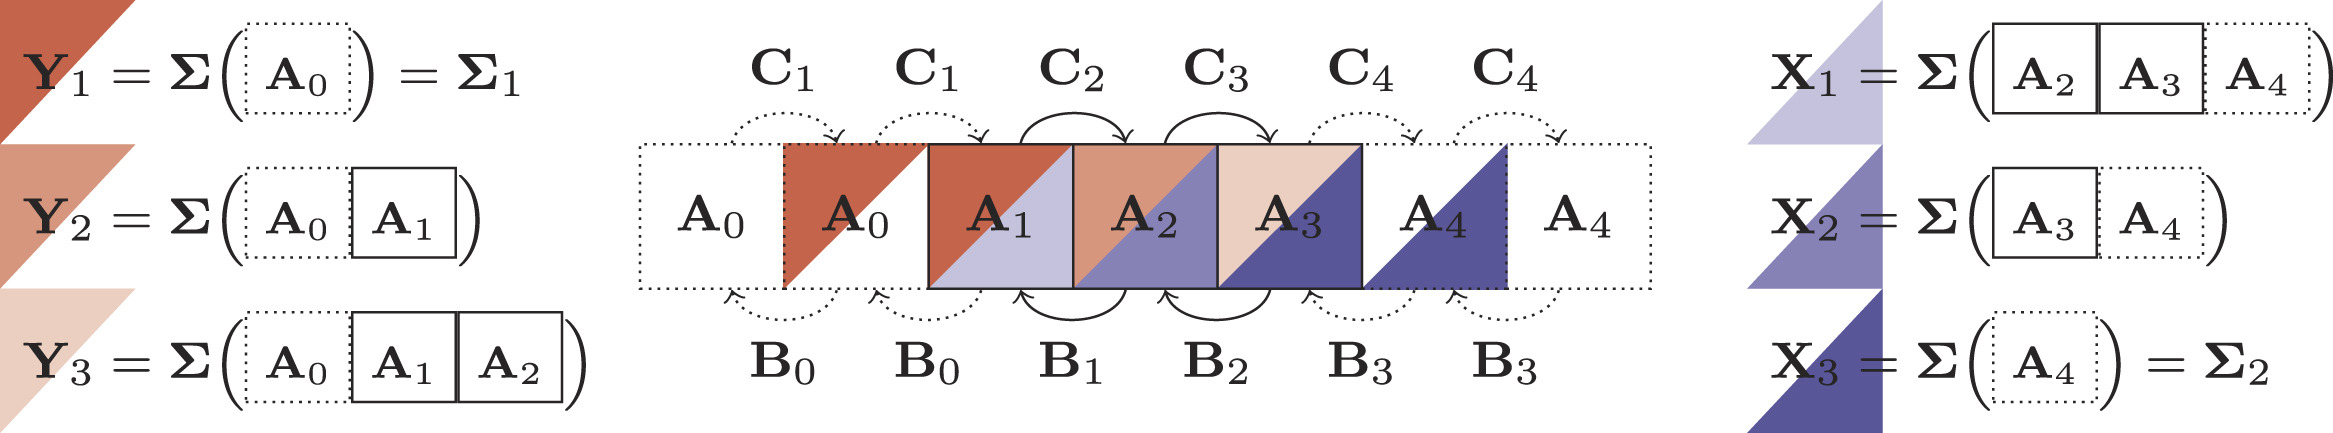
\includegraphics[scale=1.25]{figs/btd.jpg}
	\caption{\textit{Fonte: \citeauthor{transiesta2}.}}
	\label{fig:btd}
\end{figure} 

Dessa forma, considerando que a inversa de $ \vb{G}^{-1} $ é em princípio definida, é possível calcular os termos $ \vb{Y}_n $ e $ \vb{X}_n $ e com isso, aplicar novamente o algoritmo de inversão sobre $ \vb{G}^{-1} $ é possível calcular, de fato, $ \vb{G} $. Aplicando as equações \eqref{eq:btd1} e \eqref{eq:btd2}, obtemos as equações para $ \vb{G} $ como ilustrado na Figura \ref{fig:btd2}. Assim, esse método facilita o cálculo do produto matricial triplo da matriz densidade fora do equilíbrio. Por fim, na Figura \ref{fig:btd2} está ilustrado a performance do algoritmo BTD em comparação aos algoritmos de inversão LAPACK e MUMPS para o cálculo da matriz no equilíbrio (a) e fora do equilíbrio (b).  \cite{transiesta3}

\begin{figure}[h!]
	\centering
	\includegraphics[scale=2.0]{figs/performance.jpeg}
	\caption{\textit{Fonte: Comparação da performance dos códigos LAPACK e MUMPS em relação ao BTD na solução dos contornos no equilíbrio (a) e fora (b) para uma estrutura de grafeno composta por 24 átomos. \citeauthor{transiesta2}.}}
	\label{fig:btd2}
\end{figure} 


\begin{comment}
\section{Funções de Green no Equilíbrio\label{cap:fora}}

As funções de Green são definidas como as soluções de equações diferenciais inomogêneas, cuja expressão é dada por:
$$
    \bqty{z-L(\vb{r})}\green=\delta(\vb{r}-\vb{r'})
$$
sujeito à condições de contorno situadas na superfície $S$ do domínio $\Omega$ de $\vb{r}$ e $\vb{r'}$. De acordo com a notação utilizada, $z$ é uma variável complexa com $\lambda\equiv Re\Bqty{z}$ e $s\equiv Im\Bqty{z}$ e $L(\vb{r})$ é um operador diferencial linear, hermitiano e que possui um conjunto de autofunções $\Bqty{\varphi_n(\vb{r})}$ que satisfazem as mesmas condições de contorno que $\green$ \cite{green}. Para obter as propriedades das Funções de Green, é mais conveniente reescrever a equação acima utilizando a notação de Dirac:
\begin{eqnarray}\label{eq:dirac}
    \pqty{z-L}G(z)&=&\mathbb{1}\delta(z)\qquad\text{onde,}\\
    \quad\green&\equiv&\mel{\vb{r}}{G(z)}{\vb{r'}}\nonumber
\end{eqnarray}

A partir da definição de Funções de Green, podemos abordar o caso de partículas livres, cuja equação é dada por:
\begin{equation}\label{eq:livre}
    i\hbar\pdv{t}\ket{\Psi_0(t)}=\mathnormal{H}_{0}\ket{\Psi_0(t)}
\end{equation}
 Onde $H_0$ representa a energia cinética das partículas. Podemos escrever essa equação em termos de um operador diferencial linear $L=i\hbar\pdv{}{t}-H_0$, de modo que:
 \begin{equation}
     L\ket{\Psi_0(t)}=f(t)\qquad\text{com}\;f(t)=0
 \end{equation}
 
 Assim, podemos associar à Equação \ref{eq:livre} dois tipos de funções de Green $G_0^r(t)$ e $G_0^r(t)$, de modo que a Equação \eqref{eq:dirac} resulta em:
 \begin{equation}
     LG_0^{r,a}(t)=\pqty{i\hbar\pdv{}{t}-H_0}G_0^{r,a}(t)=\mathbb{1}\delta(t)
 \end{equation}
 com as seguintes condições de contorno:
 \begin{eqnarray}
     G_0^r(t)&=&0,\qquad t<t_0=0\\
     G_0^a(t)&=&0,\qquad t<t_0=0
 \end{eqnarray}
 
Aplicando essas condições de contorno, as soluções das equações de movimento são dadas por:
\begin{eqnarray}
\begin{aligned}G_{0}^r(t)&=\begin{cases}
 \;-\frac{i}{\hbar}e^{-iH_0t/\hbar},\qquad& t>t_0=0\\
  \quad 0\;,\quad &t<t_0=0
\end{cases}\end{aligned}\\\begin{aligned}
 G_{0}^a(t)&=\begin{cases}
   \quad 0 \;,\quad &t>t_0=0 \\
  \quad \frac{i}{\hbar}e^{-iH_0t/\hbar},\qquad & t<t_0=0\end{cases}\end{aligned}
\end{eqnarray}

Para a condição $t>t_0=0$, $G^r_0(t)$ é proporcional ao operador de evolução temporal $U(t,t_0=0)=e^{iH_0(t-t_0)/\hbar}=e^{-iH_0t/\hbar}$. Assim, a função de Green $G^r_0(t)$ pode ser associada ao propagador do temporal do estado $\ket{\Psi_0(t)}$ de $t_0$ a $t$, sendo, portanto denominada como função de Green retardada.
\begin{equation}
    \ket{\Psi_0(t)}=i\hbar G^r_0(t,t_0)\ket{\Psi_0(t_0}
\end{equation}

Da mesma forma, para $t<t_0$, a função de Green $G^a_0(t)$ é denominada como função de Green avançada, pois relaciona o estado $\ket{\psi_0(t_0)}$ com o estado passado $\ket{\psi_0(t)}$ e atua como um propagador desse estado de um tempo $t$ no passado, até o presente $t_0$.

\begin{equation}
    \ket{\Psi_0(t)}=-i\hbar G^a_0(t,t_0)\ket{\Psi_0(t_0}
\end{equation}
\section{O Código Smeagol\label{cap:cod}}
\end{comment}



%\chapter{Metodologia}

O estudo da interface água metal foi dividido em duas etapas de simulações computacionais atomísticas: cálculos com e sem presença de um potencial externo. A primeira etapa foi realizada no código \textit{Siesta}\cite{siesta} e os cálculos envolvendo a aplicação de um potencial externo sobre a interface foram realizados no código \textit{Transiesta}\cite{transiesta1,transiesta2,transiesta3} que está baseado no \textit{Siesta}. Os elétrons do caroço foram descritos por pseudopotenciais definidos a partir do Método da Norma Conservada de \textit{Troullier-Martins} \cite{troullier_martins}. Os elétrons de valência foram expandidos em bases locais \textit{duplo-zeta polarizadas} (DZP)\footnote{Mais detalhes sobre expansões em bases atômicas localizadas e utilização de pseudopotenciais estão descritos no Apêndice \ref{apd:bases}. Os raios de corte referentes à base e ao pseudopotencial de cada elemento estão descritos no Apêndice \ref{apd:metal}.}. Em relação aos funcionais de troca e correlação, foram utilizados os funcionais PBE \cite{PBE} e VDW-BH\cite{vdw-bh}. 

Na primeira etapa, foi investigado a adsorção de duas estruturas de água, monômero e camada, sobre superfícies metálicas de Pd(111). Em particular, foi realizado primeiramente uma análise sistemática sobre parâmetros fundamentais em um cálculo atomístico, tais como a base atômica, o pseudopotencial, o funcional de troca e correlação, o tamanho da célula unitária e a quantidade de pontos k. Em seguida, foram investigadas as interações entre a água e o metal, além das interações do tipo água-água, através da minimização do sistema. Para isso, utilizou-se o algoritmo de otimização \textit{Gradiente Conjugado} com o critério de convergência para a força de $0.005\,\si{\eV}/\si{\angstrom}$ para os monômeros com orientações perpendiculares à superfície (\textit{down} e \textit{up}) e camadas de água; para o monômero orientado paralelamente ao metal (\textit{flat}) o critério foi de $0.001\,\si{\eV}/\si{\angstrom}$. O espaçamento da malha no espaço real foi de 500 Ryd. Uma vez obtida as coordenadas minimizadas, analisou-se a estabilidades das estruturas adsorvidas através das medidas geométricas, energias de adsorção e modos normais de vibração. 

Na segunda parte, utilizamos o formalismo de NEGF com DFT para aplicar uma diferença de potencial à interface água/metal, cujas superfícies metálicas foram o Pd(111) e Au(111). Por meio dessa metodologia, analisamos como as propriedades eletrônicas e vibracionais -- obtidas anteriormente para o sistema em equilíbrio -- são modificadas na presença de um potencial externo. Nessa abordagem o sistema contendo a região central e os eletrodos metálicos se encontram fora do equilíbrio termodinâmico e os eletrodos são tratados como semi-infinitos. Em relação à superfície metálica de Au, os eletrodos construídos possuíam 3 camadas com 12 átomos em cada camada ao passo que, para o sistema constituído de Pd, os eletrodos eram compostos por 6 camadas. Essa diferença no número de camadas é devido ao tamanho da base necessária para descrever o Pd. As superfícies metálicas eram separadas a fim de minimizar as interações por um vácuo de $20\,\si{\angstrom}$ no caso do eletrodo de Au e $25\,\si{\angstrom}$ para o Pd. 

Devido à sensibilidade em descrever o sistema fora do equilíbrio é necessário minimizá-lo, primeiramente, por meio de um cálculo periódico no equilíbrio até atingir o critério de força de $0.005\,\si{\eV}/\si{\angstrom}$ - como esquematizado na Figura \ref{fig:neq_flux}. Uma vez minimizado o sistema, iniciavam-se os cálculos fora do equilíbrio obtendo-se a matriz hamiltoniana e de \textit{overlap} dos eletrodos por meio de um cálculo de \textit{bulk}. Com isso, determinava-se a correção do potencial de Hartree necessário para alinhar o potencial do sistema completo com os eletrodos. Essas foram as etapas preliminares realizadas para as superfícies metálicas de Au e Pd, nos quais eram adsorvidos uma molécula ou uma camada de água. 

Em seguida, o sistema era minimizado na situação fora do equilíbrio com o potencial externo de $ 0.0\,\si{\eV} $ aplicado. Isso permitiu comparar as diferenças provocadas na interface água/metal ao descrever o metal como semi-infinito ou finito e periódico. Após essa etapa, o sistema era minimizado com o potencial externo sendo aplicado e variando entre $ V $\footnote[7]{O valor de V considerado corresponde ao potencial aplicado sobre cada eletrodo e equivale à metade do potencial total. Assim, os valores de potenciais utilizados correspondem a V/2. A mesma observação se aplica para a seção de Resultados.}=-5 a $\,5\,\si{\eV} $. Com as coordenadas minimizadas, os modos normais de vibração eram calculados pelo método de diferenças finitas \cite{phonons}. A presença de possíveis transferências de carga entre a água e o metal, bem como as interações existentes foram estudadas por meio da diferença de densidade de carga entre o potencial aplicado e o potencial igual a $ 0.0\,\si{\eV} $.

\begin{figure}[h!]
	\centering
	\caption{Fluxograma ilustrando o processo utilizado para estudar a interface água/metal no código Transiesta.}
	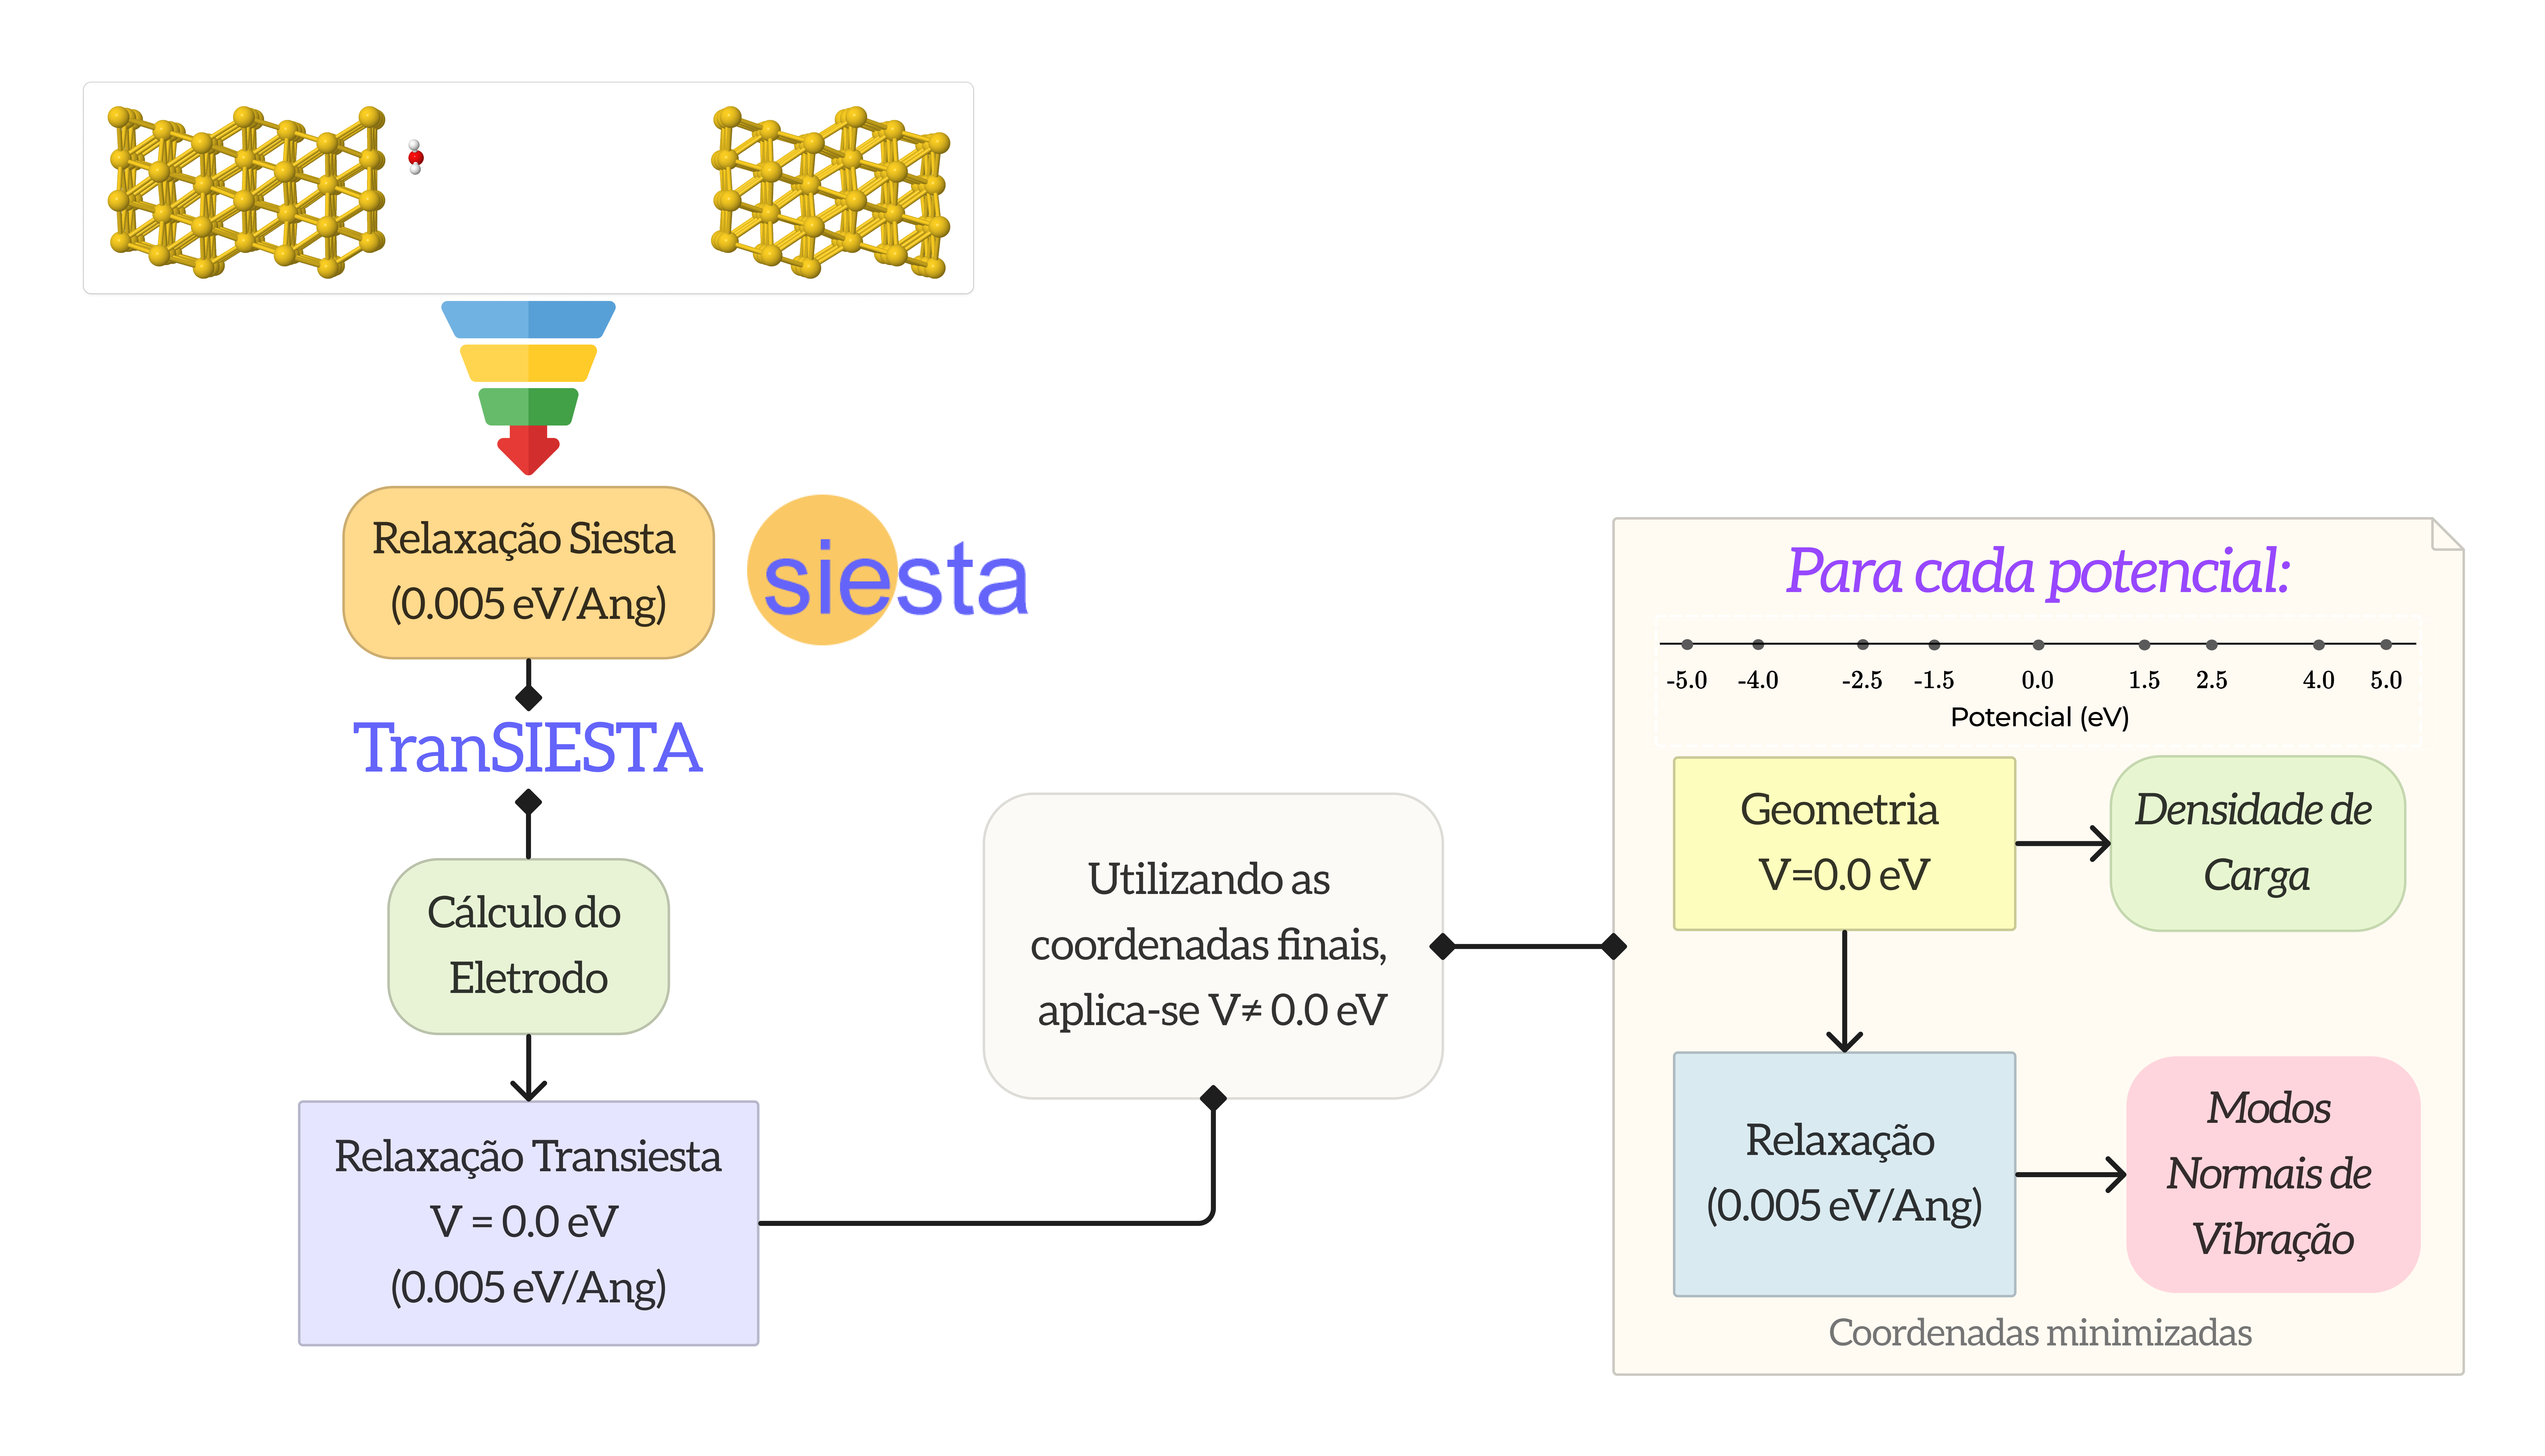
\includegraphics[scale=0.1]{figs/neq_fluxo.png}
	\legend{Fonte: compilação da autora.}
	\label{fig:neq_flux}
\end{figure} 


%Por meio das etapas descritas acima, faremos uma análise detalhada sobre o impacto da escolha de parâmetros fundamentais em um cálculo atomístico, tais como a base atômica, o pseudopotencial, o funcional de troca e correlação, o tamanho da célula unitária e a quantidade de pontos k. Além disso, obteremos parâmetros macroscópicos tais como valor da Função Trabalho e microscópicos - Modos Normais de Vibração - mediante cálculos de primeiros princípios.



%




% ----------------------------------------------------------
% Parte de revisão de literatura
% ----------------------------------------------------------
\part{Metodologia\label{cap:metodologia}}
%



% ---
% Capitulos:
% ---


\chapter{Metodologia}

O estudo da interface água metal foi dividido em duas etapas de simulações computacionais atomísticas: cálculos com e sem presença de um potencial externo. A primeira etapa foi realizada no código \textit{Siesta}\cite{siesta} e os cálculos envolvendo a aplicação de um potencial externo sobre a interface foram realizados no código \textit{Transiesta}\cite{transiesta1,transiesta2,transiesta3} que está baseado no \textit{Siesta}. Os elétrons do caroço foram descritos por pseudopotenciais definidos a partir do Método da Norma Conservada de \textit{Troullier-Martins} \cite{troullier_martins}. Os elétrons de valência foram expandidos em bases locais \textit{duplo-zeta polarizadas} (DZP)\footnote{Mais detalhes sobre expansões em bases atômicas localizadas e utilização de pseudopotenciais estão descritos no Apêndice \ref{apd:bases}. Os raios de corte referentes à base e ao pseudopotencial de cada elemento estão descritos no Apêndice \ref{apd:metal}.}. Em relação aos funcionais de troca e correlação, foram utilizados os funcionais PBE \cite{PBE} e VDW-BH\cite{vdw-bh}. 

Na primeira etapa, foi investigado a adsorção de duas estruturas de água, monômero e camada, sobre superfícies metálicas de Pd(111). Em particular, foi realizado primeiramente uma análise sistemática sobre parâmetros fundamentais em um cálculo atomístico, tais como a base atômica, o pseudopotencial, o funcional de troca e correlação, o tamanho da célula unitária e a quantidade de pontos k. Em seguida, foram investigadas as interações entre a água e o metal, além das interações do tipo água-água, através da minimização do sistema. Para isso, utilizou-se o algoritmo de otimização \textit{Gradiente Conjugado} com o critério de convergência para a força de $0.005\,\si{\eV}/\si{\angstrom}$ para os monômeros com orientações perpendiculares à superfície (\textit{down} e \textit{up}) e camadas de água; para o monômero orientado paralelamente ao metal (\textit{flat}) o critério foi de $0.001\,\si{\eV}/\si{\angstrom}$. O espaçamento da malha no espaço real foi de 500 Ryd. Uma vez obtida as coordenadas minimizadas, analisou-se a estabilidades das estruturas adsorvidas através das medidas geométricas, energias de adsorção e modos normais de vibração. 

Na segunda parte, utilizamos o formalismo de NEGF com DFT para aplicar uma diferença de potencial à interface água/metal, cujas superfícies metálicas foram o Pd(111) e Au(111). Por meio dessa metodologia, analisamos como as propriedades eletrônicas e vibracionais -- obtidas anteriormente para o sistema em equilíbrio -- são modificadas na presença de um potencial externo. Nessa abordagem o sistema contendo a região central e os eletrodos metálicos se encontram fora do equilíbrio termodinâmico e os eletrodos são tratados como semi-infinitos. Em relação à superfície metálica de Au, os eletrodos construídos possuíam 3 camadas com 12 átomos em cada camada ao passo que, para o sistema constituído de Pd, os eletrodos eram compostos por 6 camadas. Essa diferença no número de camadas é devido ao tamanho da base necessária para descrever o Pd. As superfícies metálicas eram separadas a fim de minimizar as interações por um vácuo de $20\,\si{\angstrom}$ no caso do eletrodo de Au e $25\,\si{\angstrom}$ para o Pd. 

Devido à sensibilidade em descrever o sistema fora do equilíbrio é necessário minimizá-lo, primeiramente, por meio de um cálculo periódico no equilíbrio até atingir o critério de força de $0.005\,\si{\eV}/\si{\angstrom}$ - como esquematizado na Figura \ref{fig:neq_flux}. Uma vez minimizado o sistema, iniciavam-se os cálculos fora do equilíbrio obtendo-se a matriz hamiltoniana e de \textit{overlap} dos eletrodos por meio de um cálculo de \textit{bulk}. Com isso, determinava-se a correção do potencial de Hartree necessário para alinhar o potencial do sistema completo com os eletrodos. Essas foram as etapas preliminares realizadas para as superfícies metálicas de Au e Pd, nos quais eram adsorvidos uma molécula ou uma camada de água. 

Em seguida, o sistema era minimizado na situação fora do equilíbrio com o potencial externo de $ 0.0\,\si{\eV} $ aplicado. Isso permitiu comparar as diferenças provocadas na interface água/metal ao descrever o metal como semi-infinito ou finito e periódico. Após essa etapa, o sistema era minimizado com o potencial externo sendo aplicado e variando entre $ V $\footnote[7]{O valor de V considerado corresponde ao potencial aplicado sobre cada eletrodo e equivale à metade do potencial total. Assim, os valores de potenciais utilizados correspondem a V/2. A mesma observação se aplica para a seção de Resultados.}=-5 a $\,5\,\si{\eV} $. Com as coordenadas minimizadas, os modos normais de vibração eram calculados pelo método de diferenças finitas \cite{phonons}. A presença de possíveis transferências de carga entre a água e o metal, bem como as interações existentes foram estudadas por meio da diferença de densidade de carga entre o potencial aplicado e o potencial igual a $ 0.0\,\si{\eV} $.

\begin{figure}[h!]
	\centering
	\caption{Fluxograma ilustrando o processo utilizado para estudar a interface água/metal no código Transiesta.}
	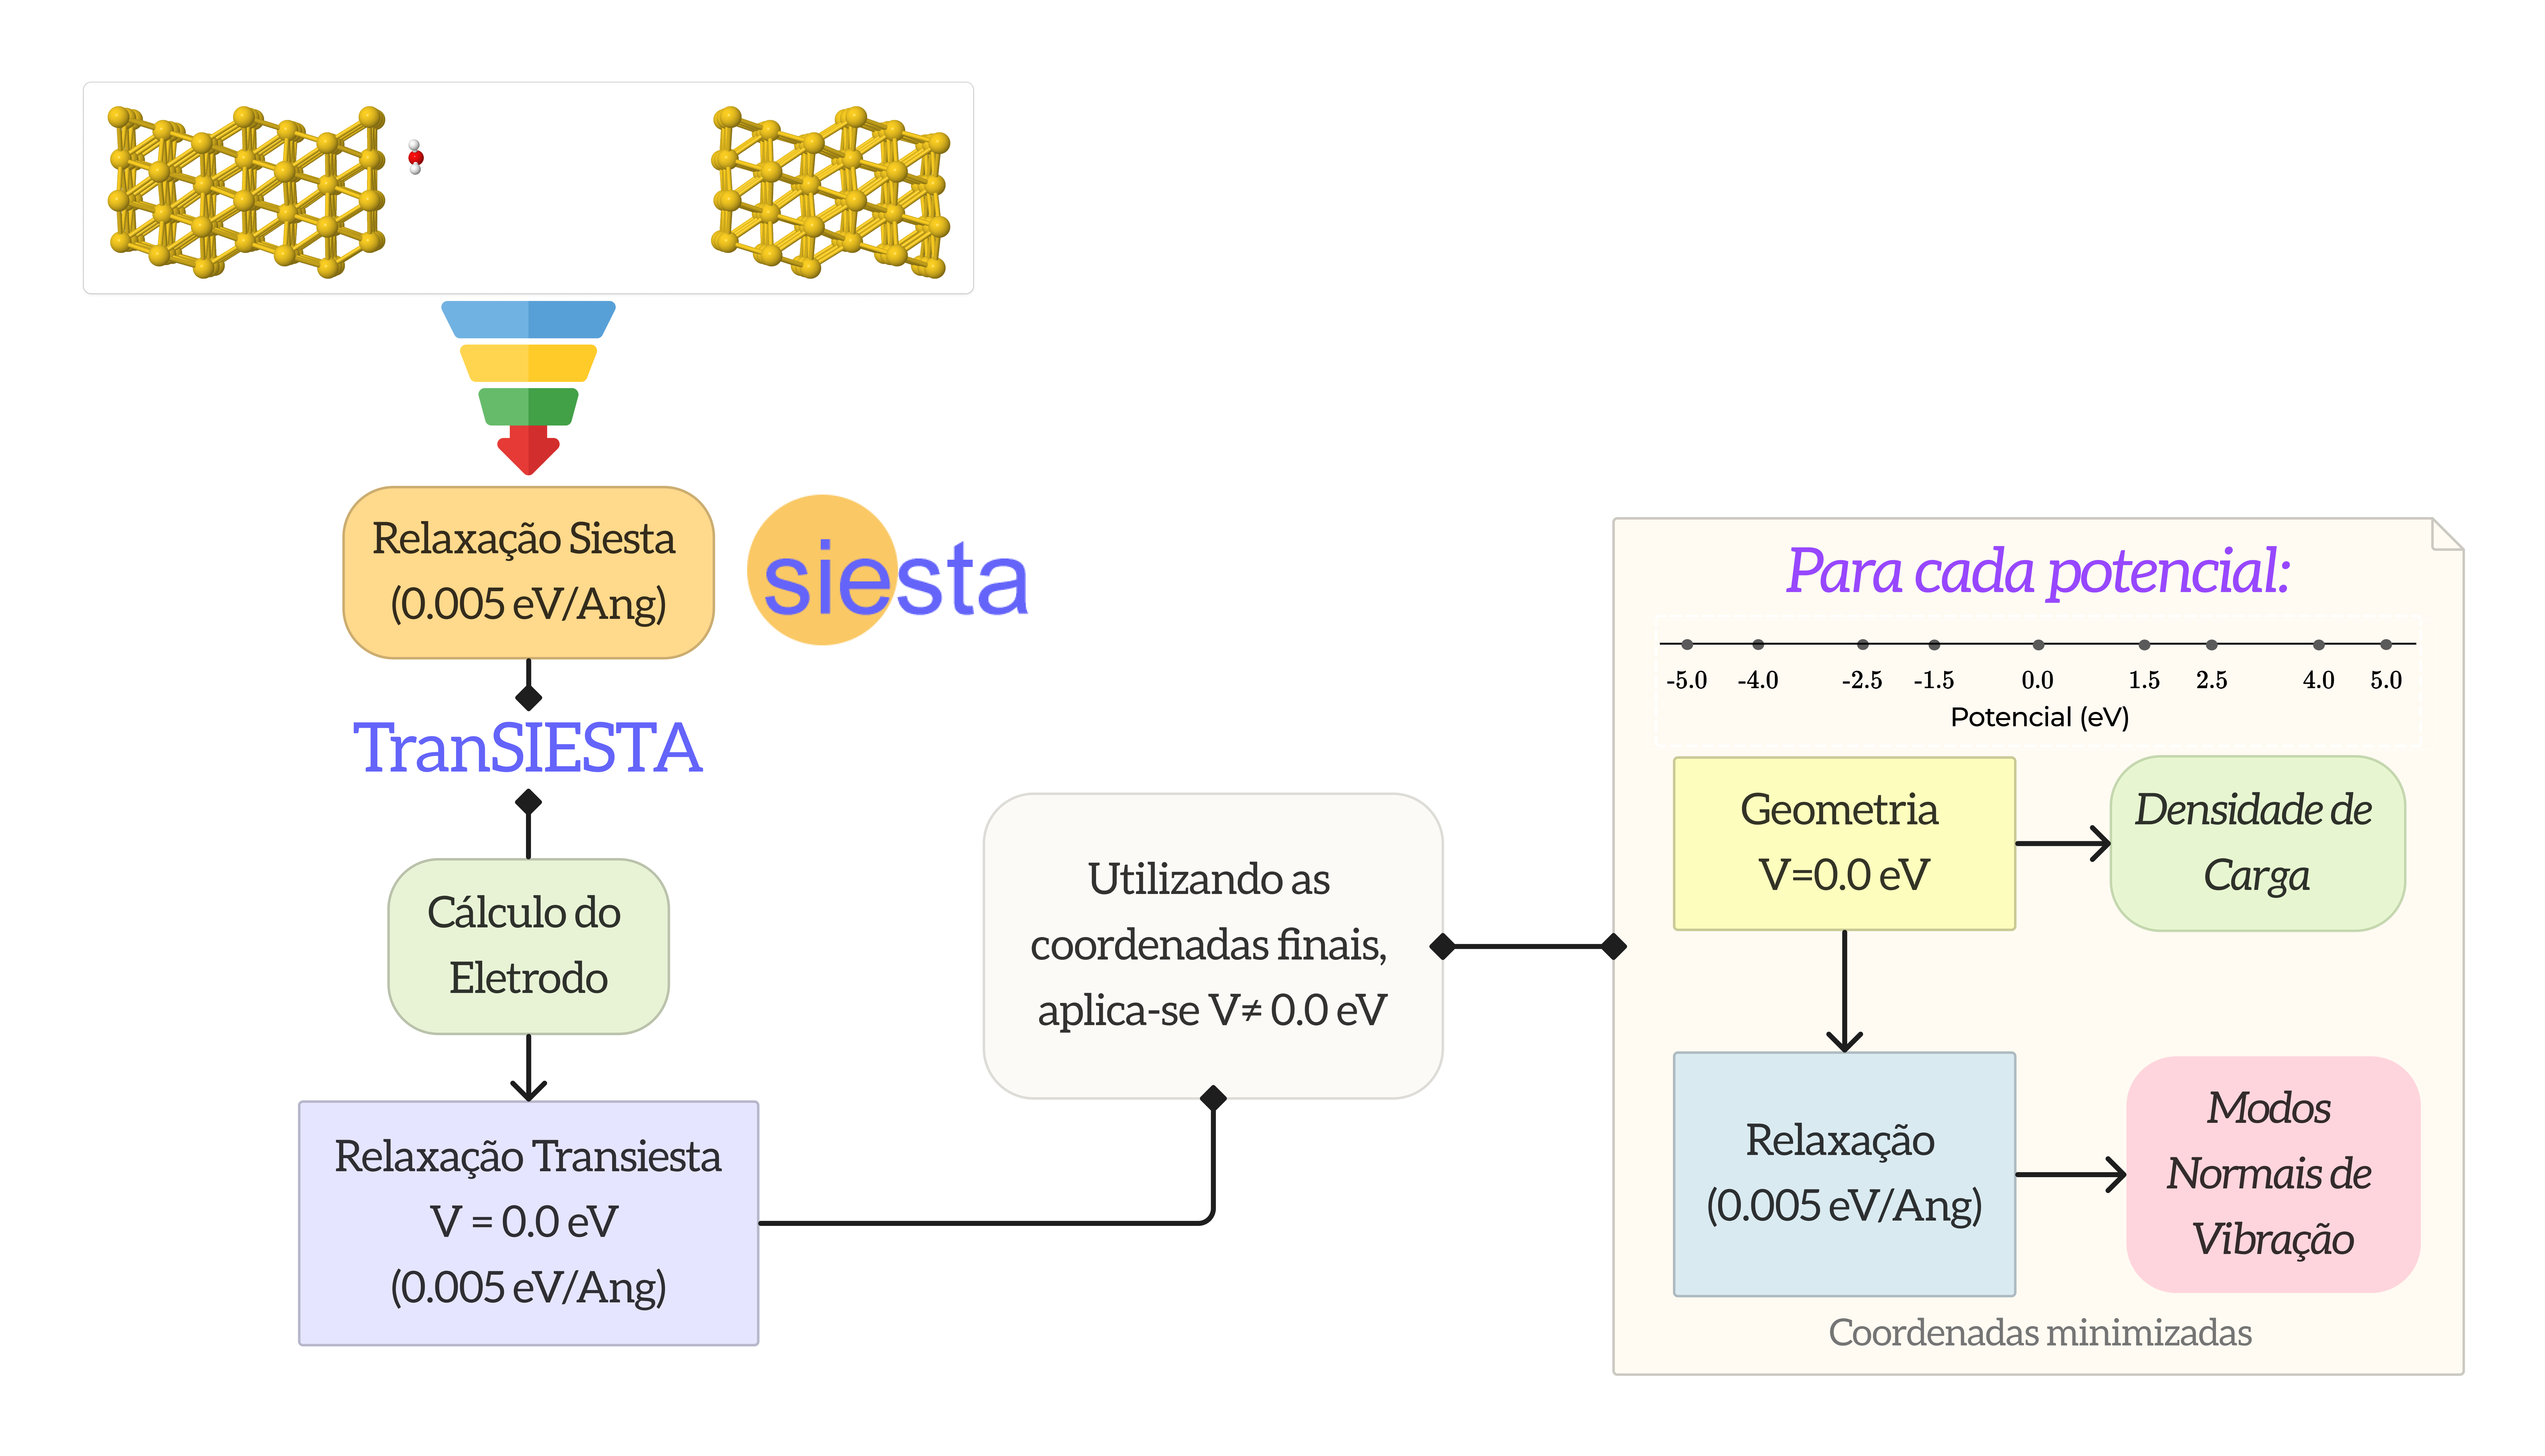
\includegraphics[scale=0.1]{figs/neq_fluxo.png}
	\legend{Fonte: compilação da autora.}
	\label{fig:neq_flux}
\end{figure} 


%Por meio das etapas descritas acima, faremos uma análise detalhada sobre o impacto da escolha de parâmetros fundamentais em um cálculo atomístico, tais como a base atômica, o pseudopotencial, o funcional de troca e correlação, o tamanho da célula unitária e a quantidade de pontos k. Além disso, obteremos parâmetros macroscópicos tais como valor da Função Trabalho e microscópicos - Modos Normais de Vibração - mediante cálculos de primeiros princípios.




% ----------------------------------------------------------
% Resultados
% ----------------------------------------------------------
\part{Resultados e Discussões}
%%M
\chapter{Interface Água/Metal \label{cap:equilibrio}}

%Nesse capítulo apresentaremos com mais detalhes os cálculos da interface água/Pd, bem como os resultados obtidos a partir das escolhas de cada etapa, tais como  a base, o pseudopotencial e o funcional de troca e correlação. Na Seção \ref{bulk} serão apresentados os detalhes computacionais utilizados nos cálculos de bulk e de slab do Pd, bem como os resultados obtidos. Uma vez caracterizadas as propriedades do metal, serão realizadas simulações com a água adsorvida no metal, com a estrutura de monômero e camada, Seção \ref{agua}. Aqui mostraremos a influência da escolha do funcional, quantidade de pontos k, tamanho da célula unitária e erro de superposição de base no valor da energia de adsorção. Por fim, na Seção \ref{sec:smeagol} construiremos a geometria do sistema para realizar os cálculos com um potencial aplicado via Funções de Green Fora do Equilíbrio (NEGF) e mostraremos os resultados preliminares.
Nesse capítulo caracterizamos a interface água/metal através das propriedades estruturais, energéticas e vibracionais de estruturas de água adsorvida no Pd(111). Para isso, estudamos a adsorção de monômero e de camada de água sobre a superfície metálica, cujos resultados estão descritos nas Seções \ref{sec:agua} e \ref{sec:re-la}, respectivamente. No primeiro sistema, a única interação existente é a do tipo água/metal, ao passo que na camada de água temos também ligações de hidrogênio entre as moléculas de água. Essas últimas podem ser impactadas pela presença de uma superfície metálica. Em particular, a intensidade dessas forças são semelhantes, de modo que, a estabilidade do sistema é definida pela competição entre os dois tipos de interação. Portanto, caracterizar as geometrias, energias e os modos vibracionais de uma estrutura adsorvida em um metal fornece detalhes sobre as interações envolvidas e sobre qual força é dominante. 

%As rotinas computacionais foram executadas pelo Siesta, onde o algoritmo de minimização utilizado foi o \textit{Gradiente Conjugado} (CG) cujo critério de convergência de força atômica variou entre 0.001 eV/\AA\ e 0.005 eV/\AA\; o \textit{Mesh Cutoff} utilizado foi de 500 Ry em todas as orientações e estruturas. Os funcionais utilizados foram GGA-PBE e VDW-BH-BH, junto à base e o pseudopotencial definidos pelos resultados da seção anterior.
%. Nesse capítulo apresentaremos os resultados do monômero (Seç. \ref{sec:agua}) e da camada de água (Seç. \ref{sec:re-la}) adsorvidos em uma superfície metálica de Pd(111).% Para isso, as posições atômicas do metal e das moléculas de água foram relaxadas, a fim de determinar . 
%Nessas simulações foram utilizadas condições periódicas de contorno com os sistemas em equilíbrio termodinâmico. 

\section{Monômero adsorvido no Pd(111) \label{sec:agua}}

% Para corrigir os Erros de Superposição de Conjuntos de Bases- \textit{Basis Set Superposition Error} (BSSE) utilizou-se o Método de Contrapeso - \textit{Atomic Counterpoise Method} (CP), no qual inseriu-se orbitais ``fantasmas'' nos cálculos de energias. Em particular, verificou-se a influência da quantidade de orbitais fantasmas no valor da energia calculada. 

\subsection*{Propriedades estruturais e eletrônicas}
Considerando-se uma molécula de água isolada, a adsorção sobre uma superfície pode ser feita por meio de diversas orientações e posições. Determinar a orientação de maior estabilidade pode fornecer informações sobre a estrutura do sistema, dissociação da molécula, resposta em relação à fatores externos e principalmente informações sobre a interação entre a molécula de água e o metal \cite{michaedelis}. Em especial, esse sistema permite estudar o papel das forças de dispersão de van der Waals na interação água-metal, visto que nesse sistema não temos formação de ligação de hidrogênio. Dessa forma, para descrever o sistema utilizamos os funcionais de troca e correlação GGA-PBE\cite{PBE} e VDW-BH\cite{vdw-bh}, no qual o primeiro  é um funcional semi-local e o segundo descreve forças de dispersão e inclui termos não-locais.

%Assim, investigamos a estabilidades de monômeros adsorvidos no Pd(111) por meio da energia de adsorção e propriedades geométricas, bem como a influência da variação do tamanho da célula unitária e da quantidade de pontos k segundo o método de \citeauthor{pontosk}. Além disso, analisamos as interações por meio da diferença de densidade de carga e pelos modos normais de vibração. Os funcionais de troca e correlação utilizados para descrever o sistema foram o . O primeiro 


Para investigar a orientação mais estável do monômero, estudamos três orientações distintas do monômero adsorvido na superfície metálica de Pd(111): \textit{flat}, \textit{down} e \textit{up}, ilustradas na Figura \ref{fig:monomer}. Na estrutura \textit{flat}, o dipolo da molécula está paralelo à superfície; na orientação \textit{down}, os átomos de H apontam para a superfície, ao passo que na orientação \textit{up} os átomos apontam para fora da superfície. Os cálculos foram feitos com condições periódicas de contorno (\textit{periodic boundary conditions}--PBC), onde as células unitárias eram compostas por 4 camadas e com repetições de $ 6\times4\times4$ e $ 4\times4\times4$ átomos metálicos no plano $ xy $ e um vácuo de $ 25\,\si{\angstrom}$ na direção z. O parâmetro de rede do Pd foi definido a partir da otimização da estrutura \textit{bulk}, onde para o funcional PBE foi obtido $3.97\,\si{\angstrom} $ e para o funcional VDW-BH $ 3.91\,\si{\angstrom} $ (vide Apêndice \ref{apd:metal}).
\begin{figure}[t!]
	\centering
	\caption{Ilustração das orientações dos monômeros de água adsorvido no Pd.}
	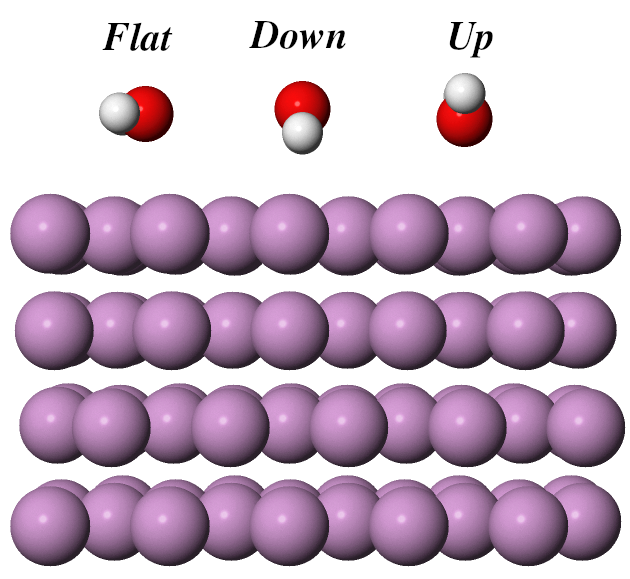
\includegraphics[scale=0.3]{figs/monomer.png}
	\legend{Fonte: Compilação da autora.}
	\label{fig:monomer}
\end{figure}  

%Para o cálculo das energias de adsorção, foi realizado um teste prévio de convergência de pontos k segundo o esquema de \citeauthor{pontosk}. Esse esquema define a quantidade de pontos finitos na primeira zona de Brillouin utilizados para calcular a densidade eletrônica do sistema no espaço recíproco. Assim, quanto mais pontos se utiliza, mais se aproxima da densidade eletrônica exata e mais caro o cálculo se torna. Assim, por meio de uma análise de convergência é possível obter o equilíbrio entre custo computacional e acurácia do resultado.

%A análise da convergência em relação à quantidade de pontos k foi realizada utilizando a configuração da molécula de água \textit{flat} junto com a célula unitária de tamanho $ 6\times4\times4 $, apenas para o funcional PBE. Primeiramente, utilizamos os seguintes esquemas de pontos: $1\times1$, $2\times2$ e $3\times3$, no qual, todo o sistema era relaxado até obter a convergência de acordo com os pontos k definidos. Em seguida, utilizamos a configuração atômica obtida com pontos k $1\times1$ e por meio de um cálculo de \textit{single point} fizemos os cálculos com os pontos k dados por: $2\times2$, $3\times3$ e $4\times4\times4$. Isso foi feito com o intuito de determinar quantos pontos k eram necessários para que os cálculos de \textit{single point} convergissem , visto que esse tipo de cálculo é mais rápido. A partir dessa análise, realizamos cálculos de \textit{single point} com o esquema $ 4\times4\times4$ para os dois tamanhos de célula unitária, as três orientações e com os funcionais PBE e VDW-BH. 
 Com o intuito de determinar as posições de equilíbrio do sistema, as rotinas computacionais foram executadas de modo que as moléculas de água e o metal eram relaxados simultaneamente. A partir da estrutura minimizada, investigou-se a estabilidade dos monômeros nas diferentes orientações e o efeito da força de dispersão através das propriedades geométricas, energia de adsorção e modos normais de vibrações. A natureza das interações entre a água e o metal foram analisadas através da diferença de densidade de carga e pelos modos normais de vibração. Além disso, examinamos a influência do tamanho da célula unitária e da quantidade de pontos k utilizados para descrever o sistema no espaço recíproco.  

A fim de mensurar o efeito do metal nas medidas geométricas, medimos os seguintes parâmetros estruturais (Figura \ref{fig:properties}) nas posições de equilíbrio:

\begin{itemize}
\item \textbf{$ \pmb{d_{OM}} $}: distância final entre o átomo de O e o metal (Pd);
\item \textbf{$ \pmb{d_{OH_1}} $ e $ \pmb{d_{OH_2}} $}: distância entre os átomos de hidrogênio ($ H_1 $ e $H_2$) e o átomo de oxigênio.% Para as moléculas na orientação \textit{down} e \textit{up}, a numeração do hidrogênio segue a convenção de que o o átomo que faz ligação de hidrogênio é o $H_2$ e o átomo livre é o $H_1$.
\item $\pmb{\Delta}$\textbf{metal}: deslocamento vertical do átomo de Pd diretamente abaixo da molécula em relação aos átomos ao redor;
\item $\pmb{\Delta Oxy}$: deslocamento lateral da molécula de água em relação ao sítio \textit{atop};
\item $\pmb{\Theta}$: ângulo final entre os átomos de hidrogênio;
\item $ \pmb{\alpha} $: inclinação final da molécula em relação à normal da superfície após o fim da simulação. Para a molécula \textit{flat}, o ângulo inicial foi 0$^{\si{\degree}}$, para a orientação \textit{down} foi de -90$^{\si{\degree}}$ e para a molécula \textit{up} foi 90$^{\si{\degree}}$.
\end{itemize}


\begin{figure}[t!]
	\centering
	\caption{Propriedades geométricas analisadas de um monômero adsorvido no Pd.}
	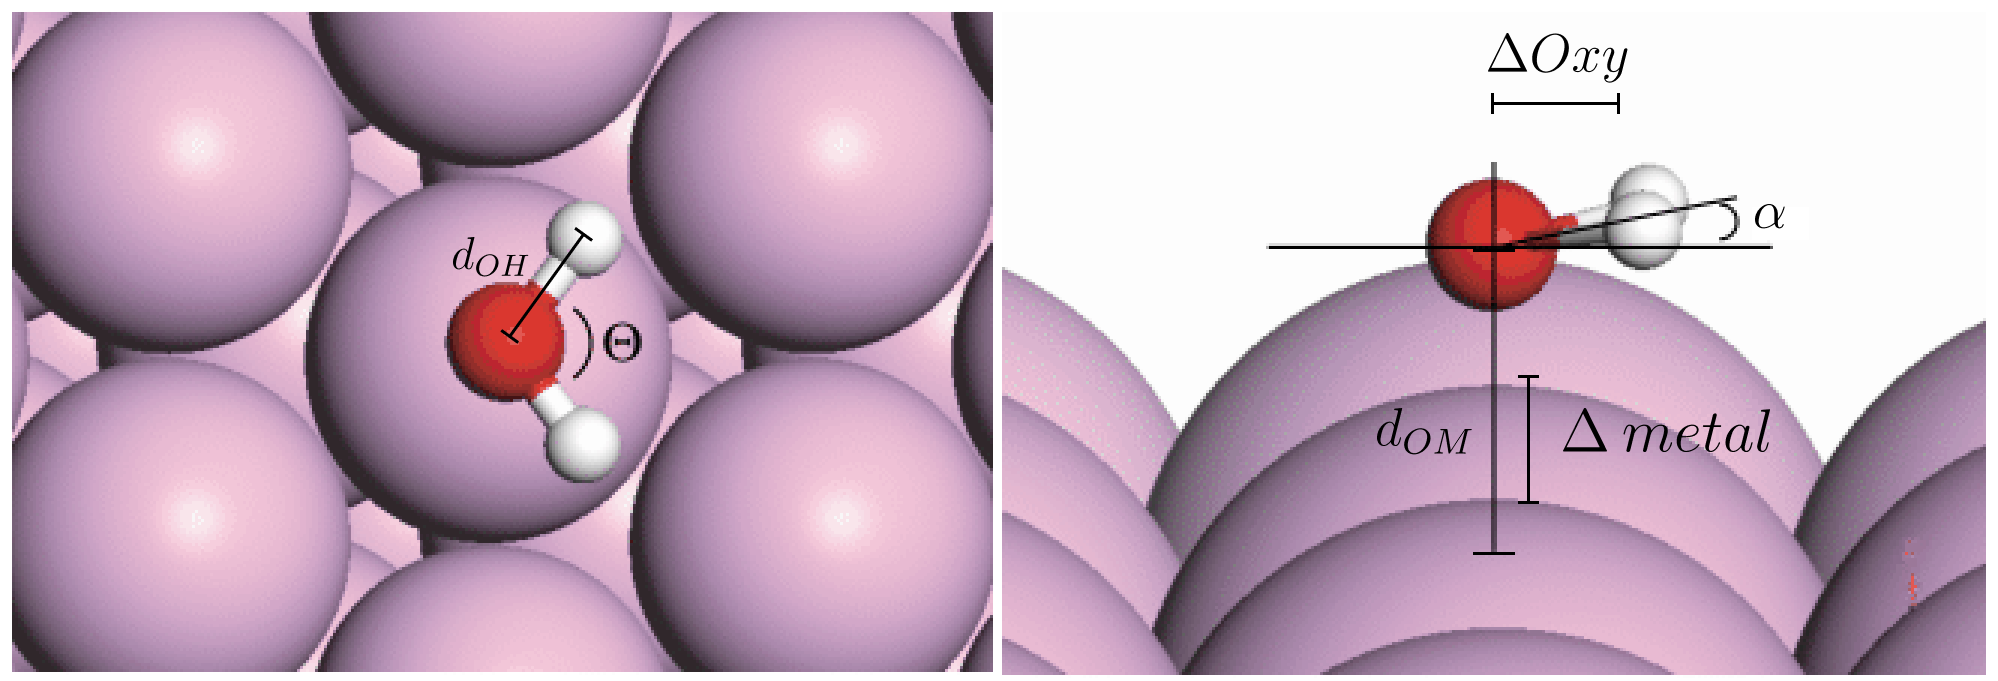
\includegraphics[scale=0.45]{figs/properties.png}
	\legend{Fonte: Adaptado de \citeauthor{michaedelis}.}
	\label{fig:properties}
\end{figure}

Primeiramente, obtivemos as medidas intramoleculares $ d_{OH} $ e $ \Theta $ para o monômero isolado, os quais estão de acordo com os valores experimentais, vide Tabela \ref{tab:isolado}. Em relação ao monômero adsorvido no metal, Tabela \ref{tab:geom_pbe}, observamos um alongamento da distância $ d_{OH} $ para as moléculas \textit{flat} e \textit{down} comparada com a molécula isolada\footnote{Na Tabela \ref{tab:geom_pbe} aparece apenas um valor para a distância $ d_{OH} $ pois os valores $ d_{OH_1} $ e $ d_{OH_2} $ foram iguais.}. Para a molécula \textit{up} não houve diferença nas distâncias $ d_{OH} $ com o valor calculado para o monômero isolado, o que era esperado, visto que os átomos de H estão mais afastados do Pd. As orientações \textit{flat} e \textit{down} apresentam valores próximos ao do monômero isolado para o ângulo $ \Theta $, ao passo que, para a configuração \textit{up} houve um alargamento da molécula em cerca de 3$ ^{\si{\degree}} $. Portanto, observa-se que, para as orientações \textit{flat} e \textit{down} a interação com o metal ocorre pelo alargamento da ligaçao O-H, enquanto que para a configuração \textit{up} ocorre um aumento do ângulo entre os átomos de hidrogênio.

%Em particular, para a molécula \textit{flat} o valor obtido está em concordância com os valores obtidos na literatura para o funcional semi-local PW91\cite{pw91}: $ 0.98\si{\angstrom} $ \cite{michaedelis} e $ 0.977\si{\angstrom} $ \cite{monomer}. Comparando com o funcional PW91, molécula \textit{flat} manteve o ângulo $ \Theta $ próximo aos valores reportados: $ 105 ^{\si{\degree}} $ \cite{michaedelis} e 105.63$ ^{\si{\degree}} $ \cite{monomer}. 


Analisando a distância $ d_{OM}$ para os cálculos com o funcional PBE, percebe-se que o menor valor corresponde à molécula na orientação \textit{flat} adsorvida na superfície $ 6\times4\times4 $, com $ d_{OM}=2.39\,\si{\angstrom} $. Essa distância está de acordo com o valor obtido por \citeauthor{monomer} para o monômero adsorvido no Pd na orientação \textit{flat}, $ d_{OM-pbe}=2.42\,  \si{\angstrom}$ com o funcional PW91\cite{pw91}. Em relação ao funcional VDW-BH, essa distância foi menor que a obtida com o PBE $ d_{OM}=2.32\,\si{\angstrom} $ e está um pouco abaixo do resultado $d_{OM-vdw}=2.48 \,\si{\angstrom}$ encontrado por \citeauthor{adrien} para o funcional DRSLL \cite{DRSLL}. %Esses resultados corroboram com os registros da literatura, os quais dizem que a orientação \textit{flat} é a mais estável.

 Além disso, observamos o efeito que o tamanho da célula provoca na distância de equilíbrio entre a água e o metal $ d_{OM} $, visto que a célula de maior tamanho apresentou as menores distâncias comparadas à célula de tamanho $ 4\times4\times4$. Isso ocorreu em todos os casos e com variações entre $ 0.01\,\si{\angstrom} $ a $ 0.12\,\si{\angstrom} $ entre as diferentes células. Esses resultados estão de acordo com o trabalho conduzido por \citeauthor{adrien}, onde os autores mostram o impacto do tamanho da célula unitária em cálculos PBC devido a falsas interações eletrostáticas que surgem entre as células vizinhas. O efeito dessas interações fictícias é observado também nos valores de $ \Delta Oxy $, no qual a molécula adsorvida na célula menor se afasta mais do sítio \textit{atop}, como por exemplo, para a orientação \textit{flat} os valores de $ \Delta Oxy $ diminuem $ \sim 0.2\,\si{\angstrom} $ ao utilizar a célula de tamanho $ 6\times4\times4 $.
   
 \begin{table}[t!]
	\centering
	\caption{Medidas da distância $ d_{OH} ( \si{\angstrom})$ e do ângulo $ \Theta $, em graus ($^{{\si{\degree}}}$) para o monômero isolado de acordo com o funcional e o valor experimental.\label{tab:isolado}} 
	\begin{threeparttable}
		\begin{tabular}{cccccc} 
			\hline\hline\addlinespace[3.6pt]
			\multicolumn{6}{c}{\textbf{Monômero Isolado}}                                                                                                                                                                                      \\ 
			\midrule
			& PBE    &  & VDW-BH    &  & Exp.\tnote{*}  \\ 
			\midrule
			$ d_{OH} $ & 0.968  &  & 0.970  &  & 0.957                                                                                                                                                                    \\
			$\Theta$    & 103.90 &  & 103.90 &  & 104.52                                                                                                                                                                   \\
			\hline\hline
		\end{tabular}
		\begin{tablenotes}\footnotesize
			\item[*] \citeauthor{agua_exp}
		\end{tablenotes}
		\legend{Fonte: Compilação da autora}
	\end{threeparttable}
\end{table}
\begin{table}[h!]
	\centering
	\caption{Tabela contendo as medidas geométricas do monômero adsorvido no Pd para o funcional PBE e VDW-BH para diferentes tamanhos de superfície. As medidas analisadas foram a distância entre os átomos de O e Pd ($ d_{OM} $) e O e H ($ d_{OH} $), além das variações das distâncias em relação à posição inicial da água ($ \Delta Oxy $) e em relação aos átomos adjacentes ($ \Delta metal$), todas fornecidas em $\,\si{\angstrom}$. Ademais foram analisados o ângulo entre os átomos de H ($ \Theta $) e a inclinação da molécula em relação à superfície de Pd ($ \alpha $), onde ambas medidas estão em graus ($^{\si{\degree}} $).\label{tab:geom_pbe}}
	\begin{tabular}{ccccccccc} 
		\hline\hline\addlinespace[3.6pt]
		\multicolumn{9}{c}{\textbf{Propriedades Estruturais}}   \\\midrule
		\multicolumn{9}{c}{\textbf{Funcional PBE}}                                                                                                                            \\      	\midrule
		\multirow{2}{*}{}                 & \multicolumn{2}{c}{Flat}              &  & \multicolumn{2}{c}{Up}                &  & \multicolumn{2}{c}{Down}               \\ 
		\cmidrule{2-3}\cmidrule{5-6}\cmidrule{8-9}
		& $4\times4\times4$ & $6\times4\times4$ &  & $4\times4\times4$ & $6\times4\times4$ &  & $4\times4\times4$ & $6\times4\times4$ \\
		\midrule
		$ d_{OH} $           & 0.98              & 0.98              &  & 0.97              & 0.97              &  & 0.98              & 0.98               \\	
		$\Theta$                & 104               & 104               &  & 107               & 107               &  & 103               & 103                \\ 
		
		$ d_{OM} $         & 2.51              & 2.39              &  & 2.49              & 2.41              &  & 3.08              & 3.05               \\ 
		

		$\Delta metal$ & 0.04            &
		0.04           &  & 0.04              & 0.04  &  & -0.04              & -0.03               \\ 
		
		$\Delta Oxy$   & 0.34              & 0.14              &  & 0.08             & 0.03              &  & 0.12              & 0.03               \\ 
		$\alpha$           	     &   2                &           -2        &  &     94              &           92        &  &     -90              &    -90                \\
		\midrule \multicolumn{9}{c}{\textbf{Funcional VDW-BH}}                                                                                                                            \\ \midrule	
		$ d_{OH} $            & 0.98              & 0.98              &  & 0.97              & 0.97              &  & 0.98              & 0.98               \\	
		$\Theta$              & 104               & 104               &  & 107               & 108              &  & 103               & 104                \\ 
		$ d_{OM} $ & 2.43            & 2.32              &  & 2.40              & 2.33              &  & 2.98             & 2.97\\ 

		$\Delta metal$  & 0.03            & 0.03             &  & 0.03              & 0.02              &  & -0.05             & -0.04               \\ 
		
		$\Delta Oxy$    & 0.31              & 0.08             &  & 0.07             & 0.02              &  & 0.13              & 0.04               \\ 
		
		$\alpha$      	     &   -2                &           -5        &  &     94              &           92        &  &     -92              &    -90                \\
	

		\hline\hline
	\end{tabular}
	\legend{Fonte: compilação da autora.}
\end{table}

 Ademais, a configuração \textit{up} apresentou valores próximos à distância $ d_{OM} $ da molécula \textit{flat}, o que era esperado pois na orientação \textit{up} os átomos de hidrogênio estão apontando para fora da superfície, de modo que o oxigênio, que é mais eletronegativo que o paládio, é atraído para superfície metálica. De forma oposta ocorre para a orientação \textit{down}, cuja distância O-Pd é maior pois os átomos de hidrogênio estão apontados para o Pd. Essas afirmações são evidenciadas pelo deslocamento vertical do átomo de Pd ($ \Delta metal $) situado diretamente abaixo da monômero, onde as configurações \textit{down} apresentam variações negativas, ou seja, esse átomo de Pd está verticalmente mais afastado da molécula em relação aos átomos de Pd ao redor; para as orientações \textit{up} e \textit{flat} as variações são positivas, logo o átomo de Pd está mais próximo à molécula. O deslocamento $ \Delta metal $ da orientação flat que encontramos para o funcional PBE foi de $0.04\;\AA$ e está próximo ao valor registrado por \citeauthor{michaedelis} para o funcinal PW91, $ \Delta metal_{ref}=0.03\,\si{\angstrom} $. 
 
 
 Analisando a inclinação entre o plano do dipolo da molécula ($ \alpha $) e a superfície metálica, observa-se variações entre $ 2^{\si{\degree}} $ a $ 5^{\si{\degree}} $ em relação à orientação inicial. Para a molécula \textit{flat}, as inclinações obtidas nesse estudo foram menores que os ângulos de $ 7^{\si{\degree}} $ e $ 20^{\si{\degree}} $ obtidos com o funcional PW91 nos estudos \cite{michaedelis} e \cite{monomer}, respectivamente. Vale notar que em relação às propriedades geométricas aqui analisadas não houveram diferenças significativas entre os valores obtidos com o funcional VDW-BH e PBE. Isso é interessante, pois reflete a capacidade do funcional PBE em descrever a geometria do sistema, ainda que esse funcional não seja sensível à interações de dispersão e consequentemente não descreva satisfatoriamente a estrutura da água líquida \cite{vdw-func,review_new}.% Isso foi também observado por \citeauthor{vdw-func} ao observar que os funcionais da  vários funcionais da família VDW-BH e  que fornece geometrias próximas ao PBE e valores de energias mais estáveis. 
 
Uma vez caracterizado o efeito da adsorção sobre a geometria do sistema, analisamos a estrutura eletrônica da interface água/metal. A energia de adsorção corresponde ao decréscimo de energia que ocorre quando um material (adsorvato) é adsorvido em outro (adsorvente):
\begin{equation}
	E_{ads}=-\bqty{E_{Pd+H_{2}O}-\pqty{E_{Pd}+E_{H_2O}}}
\end{equation}
ou seja, o negativo da energia do sistema composto subtraído da energia dos sistemas separados. Nessa definição as coordenadas dos sistemas individuais correspondem às coordenadas minimizadas do sistema composto e valores mais altos de energia descrevem processos de adsorção mais favoráveis (endotérmicos) \cite{vdw-func}. Ao calcular a energia dessa forma descreve-se somente as bases específicas de cada componente, como por exemplo, no cálculo de $ E_{Pd} $ apenas a base do Pd está presente. Logo, os efeitos de superposição entre as bases que descrevem os átomos do metal e da água são ignorados. Assim, para corrigir erros de superposição de bases (\textit{basis set superposition error}--BSSE), utiliza-se \textit{orbitais fantasmas} para descrever as bases vazias dos átomos. Esse método pode ser traduzido pela expressão seguinte, onde os índices superiores indicam a base utilizada e os índices inferiores referem-se às geometrias.
\begin{equation}
	E_{ads}^{BSSE}(r)=-\bqty{E_{Pd+H_2O}^{Pd+H_2O}(r)-\pqty{E_{Pd}^{Pd+H_2O}(r)+E_{H_2O}^{Pd+H_2O}(r)}}.
\end{equation}

Como foi visto anteriormente, o tamanho da célula no espaço real afeta a geometria do sistema e está relacionado à quantidade de pontos k necessários para descrever a densidade eletrônica no espaço recíproco. Assim, quanto maior a quantidade de pontos k, mais a solução se aproxima da densidade eletrônica correta e mais demorado o cálculo se torna computacionalmente. Para definir o equilíbrio entre custo computacional e acurácia do resultado, realizou-se um teste de convergência a fim de definir a quantidade de pontos k necessários para obter a convergência na energia de adsorção.  
 \begin{figure}[b!]
	\centering
	\caption{Gráfico da Energia de Adsorção (eV) em função da quantidade de pontos k considerando a correção dos erros de BSSE (linha tracejada) e sem correção (linha sólida) para a molécula \textit{flat} adsorvida na superfície $ 6\times4\times4 $. Nos dois casos, a energia converge a partir de $ 2\times2 $ pontos k.}
	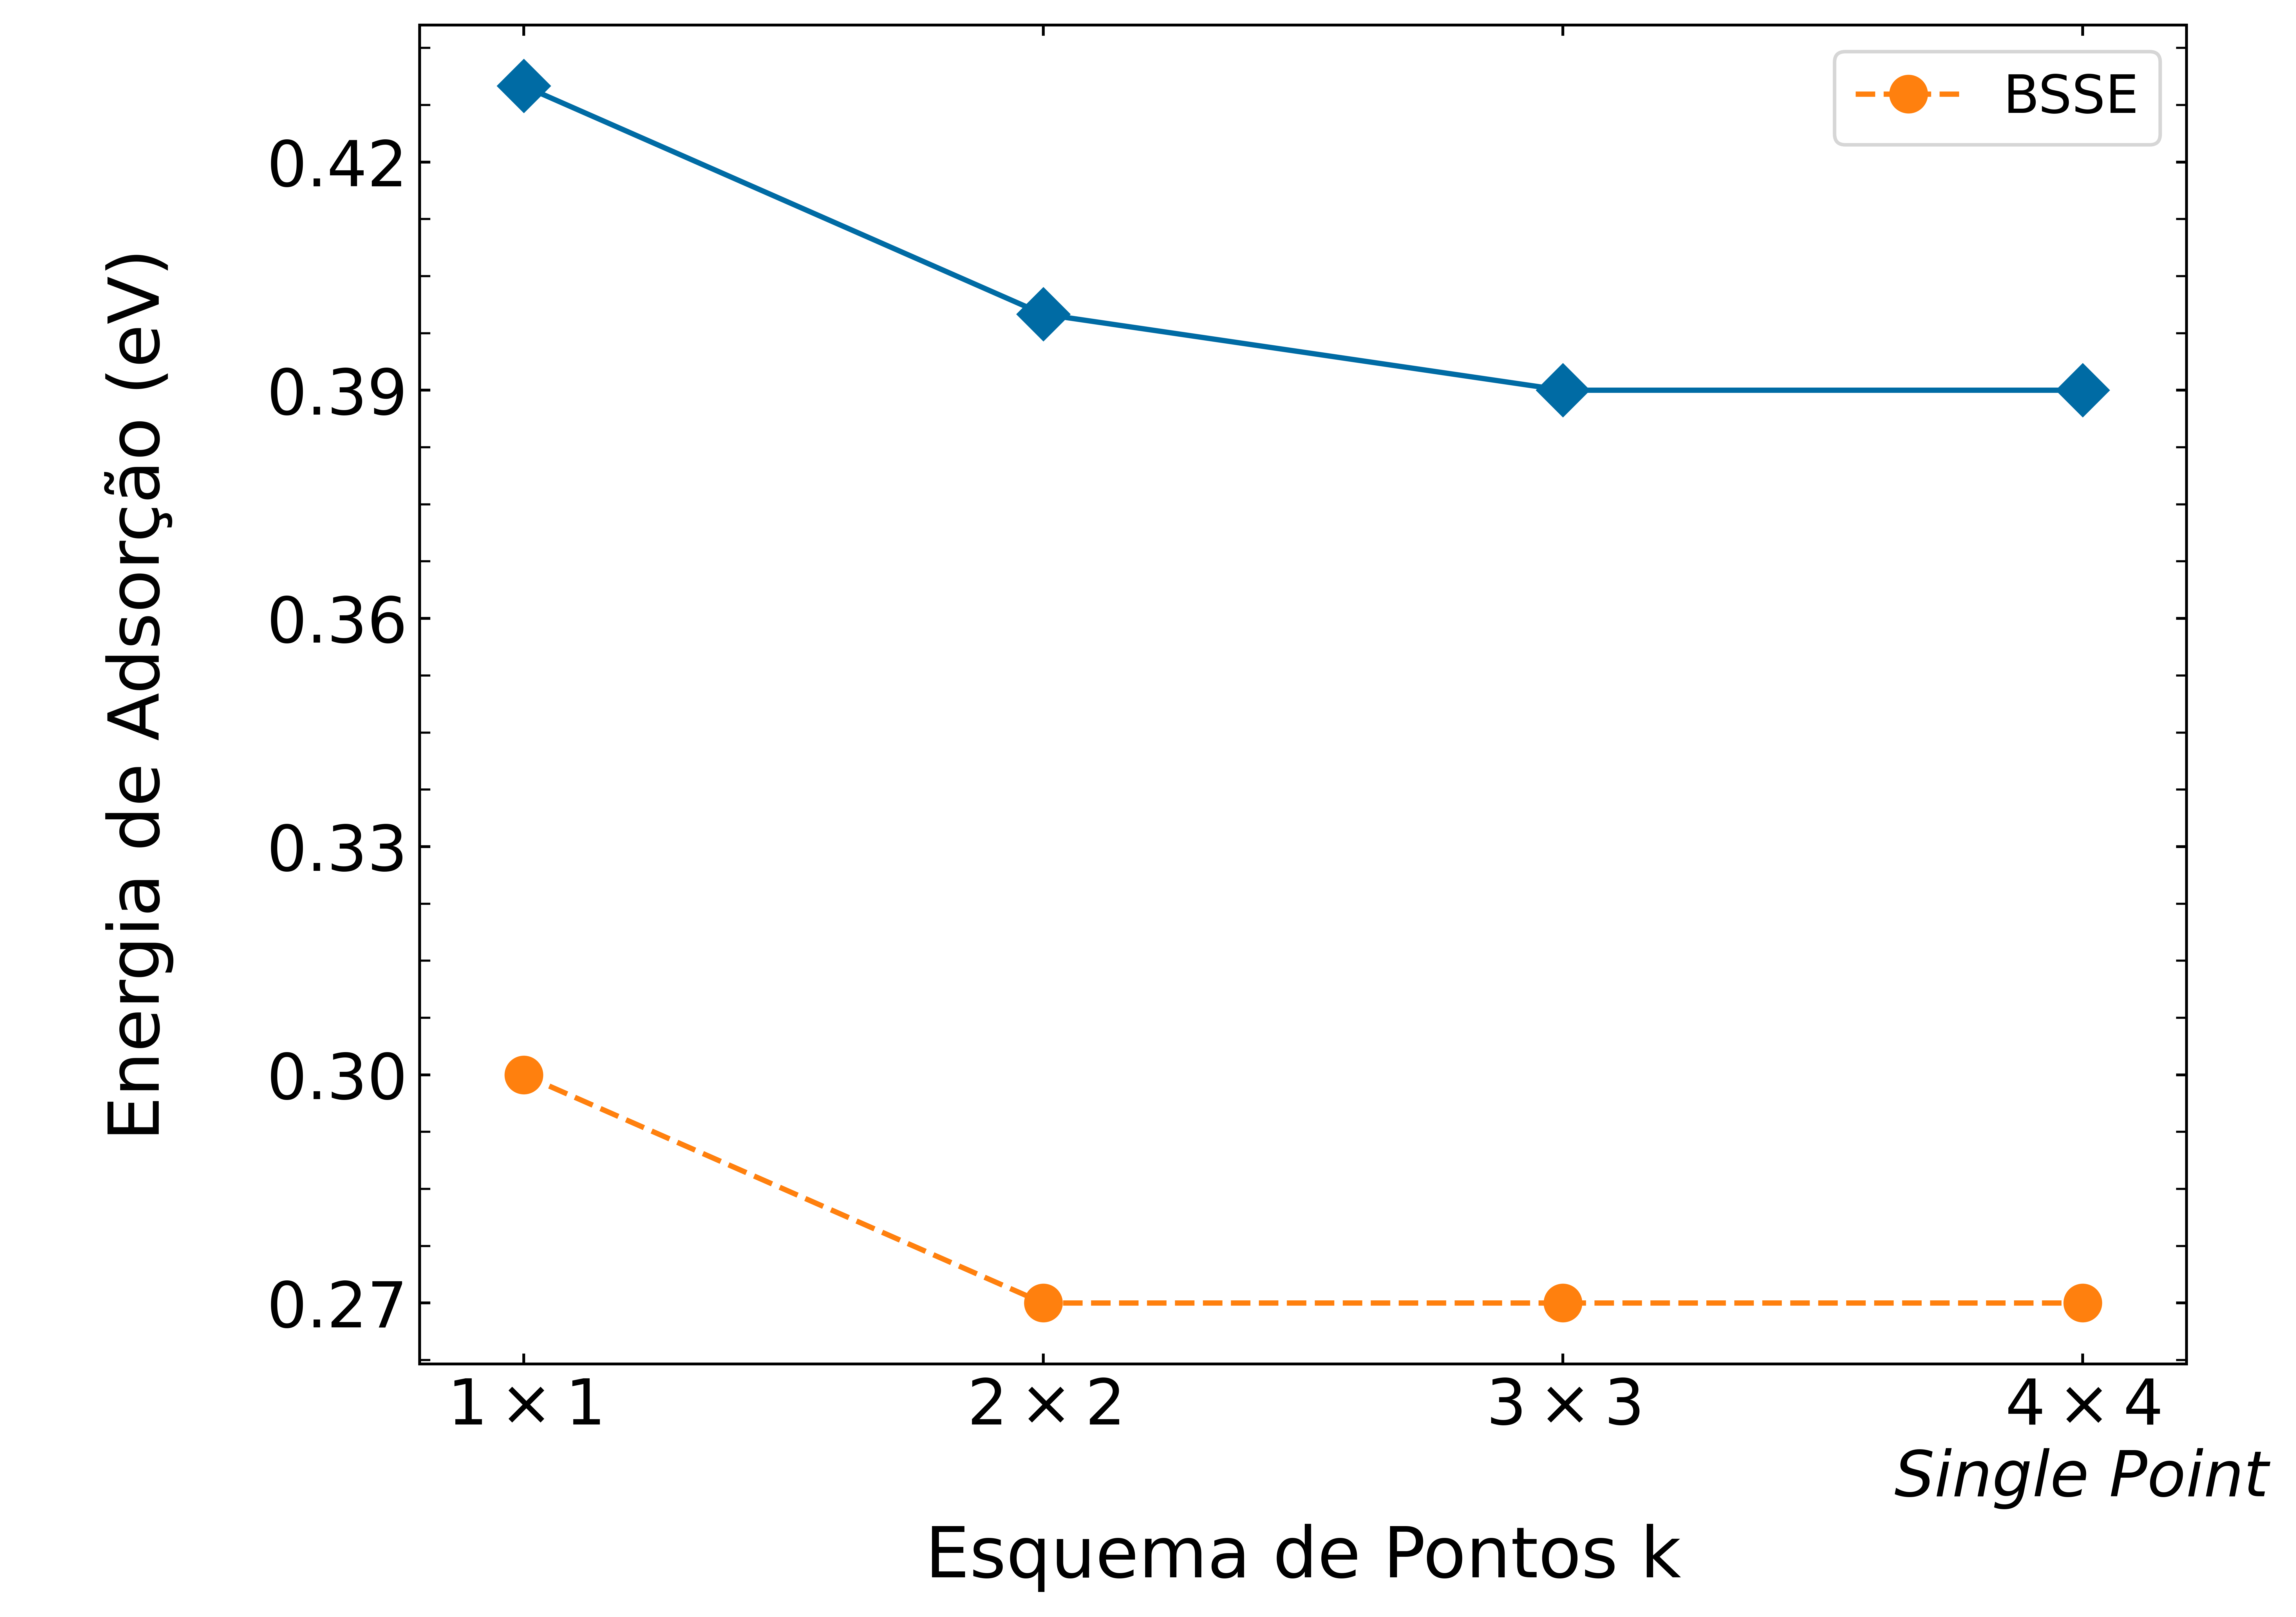
\includegraphics[scale=0.5]{figs/converg.png}
	\legend{Fonte: compilação da autora.}
	\label{fig:pontosk}
\end{figure}
 
Essa análise foi realizada utilizando a configuração da molécula de água \textit{flat} adsorvida na superfície metálica de tamanho $ 6\times4\times4 $ com o funcional PBE. Para isso realizou-se a minimização do sistema para cada conjunto de pontos k: $1\times1$, $2\times2$ e $3\times3$ (Figura \ref{fig:pontosk}). Assim, observa-se que a convergência foi alcançada a partir de $ 2\times2 $ pontos k, seja com a correção BSSE ou sem. Ademais observamos que a presença da correção BSSE fornece uma melhoria nos valores de energia de $ 0.13 \,\si{\eV} $ em relação às energias sem correção. Dessa forma, $1\times1$ pontos k descreve corretamente a geometria do sistema, mas superestima a energia de adsorção. Isso permite relaxar o sistema com o esquema de pontos $1\times1$ e em seguida, aumentar a quantidade de pontos k e obter valores de energias mais precisos.%convergidas através do aumento pontos k; como resultado, tem-se um significativo ganho em relação ao custo computacional.  
   %Em relação aos valores sem correção, a convergência é atingida a partir de $ 3\times3 $ pontos k para o cálculo de relaxação e com $ 4\times4\times4 $ pontos k para o \textit{single point}. No entanto, a partir do esquema $ 2\times2 $ já se obtém um valor bem próximo à convergência, como pode ser visto no gráfico da Figura \ref{fig:pontosk}.
 
\begin{comment}
   \begin{table}[h!]
 	\centering
 	\caption{Tabela contendo os valores das energias de acordo com a quantidade de pontos k, obtidas por meio de relaxação e single point.\label{tab:pontosk}}	
 	\begin{tabular}{ccccccc} 
 		\hline\hline
 		\multicolumn{7}{c}{\textbf{Energias de Adsorção (eV) - PBE}}                                              \\ 
 		\midrule
 		&  & \multicolumn{2}{c}{}          &  & \multicolumn{2}{c}{BSSE}                      \\ 
 		\cmidrule{3-4}\cmidrule{6-7}
 		\textit{Pontos k} &  & Relaxação & \textit{Single Point} &  & \textit{Relaxação} & \textit{Single Point}  \\ 
 		\midrule
 		$1\times1$        &  & 0.43      & -                     &  & 0.30               & -                      \\
 		$2\times2$        &  & 0.40      & 0.40                  &  & 0.27               & 0.27                   \\
 		$3\times3$        &  & 0.39      & 0.40                  &  & 0.27               & 0.27                   \\
 		$4\times4\times4$        &  & -         & 0.39                  &  & -                  & 0.27                   \\
 		\hline\hline
 	\end{tabular}
 	\legend{Fonte: compilação da autora.}
 \end{table}
\end{comment} 

Uma vez determinados os parâmetros de convergência para a molécula \textit{flat}, esses resultados foram estendidos para as orientações \textit{down} e \textit{up} adsorvidas nos dois tamanhos de superfícies - Tabela \ref{tab:energies-k}. Assim, observa-se que ao aumentar a quantidade de pontos k os valores de energia dos dois tamanho diferentes de célula unitária se aproximam. Em outras palavras, ao aumentar o número de pontos k, os valores das energias da célula menor se aproximam dos valores convergidos da célula maior. Isso pode ser ilustrado através das energias de adsorção da orientação \textit{flat} com ambos funcionais, onde as diferenças de energia entre os diferentes tamanhos de célula variavam entre $ 0.08-0.1\,\si{\eV}$ com $ 1\times1 $ pontos k e ao aumentar a quantidade de pontos k para $ 4\times4\times4 $ essas diferenças diminuem para $ 0.01-0.02\,\si{\eV} $. % Isso é observado pela menor distância $d_{OM}$ para a célula maior e também pelo fato de que,. %Analisando os valores da célula unitária de tamanho $ 4\times4\times4 $, vemos a convergência da energia quando se aumento o número de pontos k para as orientações \textit{flat} e \textit{up}, tanto para o funcional PBE, quanto para o funcional VDW-BH. 
 
 \begin{table}[b!]
 	\centering
 	 \caption{Energias de adsorção das diferentes orientações do monômero adsorvido no Pd de acordo com o funcional, quantidade de pontos-k e tamanho da célula unitária. Além disso, foi calculado as energias considerando os erros de superposição de base e a correção (BSSE).\label{tab:energies-k}}
 	\begin{tabular}{cccccccccccc} 
 		\hline\hline\addlinespace[3.8pt]
 		\multicolumn{12}{c}{\textbf{Energias de Adsorção (eV)}}                                                                                                                                          \\ 
 		\midrule
 		\multirow{3}{*}{} & \multicolumn{5}{c}{PBE}                                                          &  & \multicolumn{5}{c}{VDW-BH}                                                           \\ 
 		\cmidrule{2-6}\cmidrule{8-12} \textit{Slab}
 		& \multicolumn{2}{c}{$4\times4\times4$} &  & \multicolumn{2}{c}{$6\times4\times4$} &  & \multicolumn{2}{c}{$4\times4\times4$} &  & \multicolumn{2}{c}{$6\times4\times4$}  \\ 
 		\cmidrule{2-3}\cmidrule{5-6}\cmidrule{8-9}\cmidrule{11-12} \textit{Pontos k}
 		& $1\times1$ & $4\times4$             &  & $1\times1$ & $4\times4$                 &  & $1\times1$ &$4\times4$           &  & $1\times1$ & $4\times4$                  \\ 
 		\midrule
 		\textbf{Flat}              & 0.35      & 0.38                         &  & 0.43      & 0.39                         &  & 0.53     & 0.57                         &  & 0.63      & 0.59                          \\ 
 		
 		\textbf{Up}                & 0.24      & 0.25                     &  & 0.30      & 0.27                     &  & 0.42     & 0.44                    &  & 0.49      & 0.46                      \\ 
 		
 		\textbf{Down}              & 0.22      & 0.21                     &  & 0.23      & 0.22                     &  & 0.36     & 0.35                     &  & 0.36      & 0.35                      \\ 
 		\midrule \multicolumn{12}{c}{\textbf{Energias de Adsorção (eV) - BSSE}}                                                                                                                                          \\ \midrule
 		\textbf{Flat}              & 0.22     &          0.25                &  & 0.30      & 0.27                         &  &   0.40  &    0.44                     &  &   0.49    & 0.45                          \\ 
 		
 		\textbf{Up}                & 0.14      & 0.16 &  & 0.20      & 0.18                     &  &    0.31  &           0.34           &  &     0.38  &              0.35         \\ 
 		
 		\textbf{Down}              & 0.10      &            0.10          &  & 0.10      &              0.10        &  &    0.22  &    0.21                  &  &    0.22  &        0.21               \\
 		\hline\hline
 	\end{tabular}
 \legend{Fonte: compilação da autora.}
 \end{table}
 
Os valores das energias de adsorção associados às distâncias $ d_{OM} $ revelam que a orientação \textit{flat} é a mais estável, independentemente do funcional utilizado. Em particular, o funcional VDW-BH apresentou um aumento médio na energia de $ 0.16\,\si{\eV} $ em relação ao funcional PBE. Isso indica que a água se liga mais fortemente ao metal quando considerar forças de dispersão. De acordo com \citeauthor{adrien}, a interação água-metal possui características similares à ligação de hidrogênio. Assim, a interação água-metal pode ser entendida como uma pseudo ligação de hidrogênio entre duas moléculas de água, onde o metal se comporta como uma pseudo molécula de água. Além disso, funcionais do tipo VDW, que incluem termos de correlação não locais, tendem a ser mais sensíveis às interações desse tipo.   

Os nossos valores estão de acordo com os reportados na literatura para energia de adsorção da molécula \textit{flat} com o funcional PBE, $ E_{PBE-ref1}=0.243\,\si{\eV} $ \cite{vdw-func} e $ E_{PBE-ref2}=0.28 \,\si{\eV} $ \cite{adrien}. Para o funcional VDW-DRSLL, o valor obtido por \citeauthor{adrien} para essa orientação foi $ E_{DRSLL}=0.263\,\si{\eV} $, o que difere em cerca de $ 0.19\,\si{\eV} $ do resultado obtido para o funcional VDW-BH. Essa diferença é devido ao fato do termo de troca do funcional DRSLL ser descrito pelo rev-PBE que, por sua vez, é um funcional repulsivo que enfraquece a interação com o metal \cite{adrien}. Ao modificar o termo de troca, como feito no funcional VDW-BH e também pelos autores \citeauthor{vdw-func} ao utilizar a otimização Becke88, observa-se um melhoria na acurácia do funcional.

\begin{figure}[b!]
	\centering
	\caption{(a) Diagrama dos níveis de energia dos mais altos orbitais ocupados de uma molécula de água isolada (b) Diferenças de densidades de carga $\Delta\rho$ das moléculas \textit{up}, \textit{down} e \textit{flat} adsorvidas na superfície $6\times4\times4$ e calculadas com os funcionais PBE e VDW-BH. A diferença de densidade de carga é definida por $\Delta\rho=\rho_{H_2O+Pd}-(\rho_{H_2O}+\rho_{Pd})$. Para todos os casos, o valor da isosuperfície foi $1.06\times10^{-3}\;e/\AA$, onde vermelho (azul) indica uma diminuição (aumento) da densidade de carga durante a adsorção.}
	\begin{subfigure}{0.38\textwidth}            
		\caption{\textit{Monômero Isolado}}
		\centering
		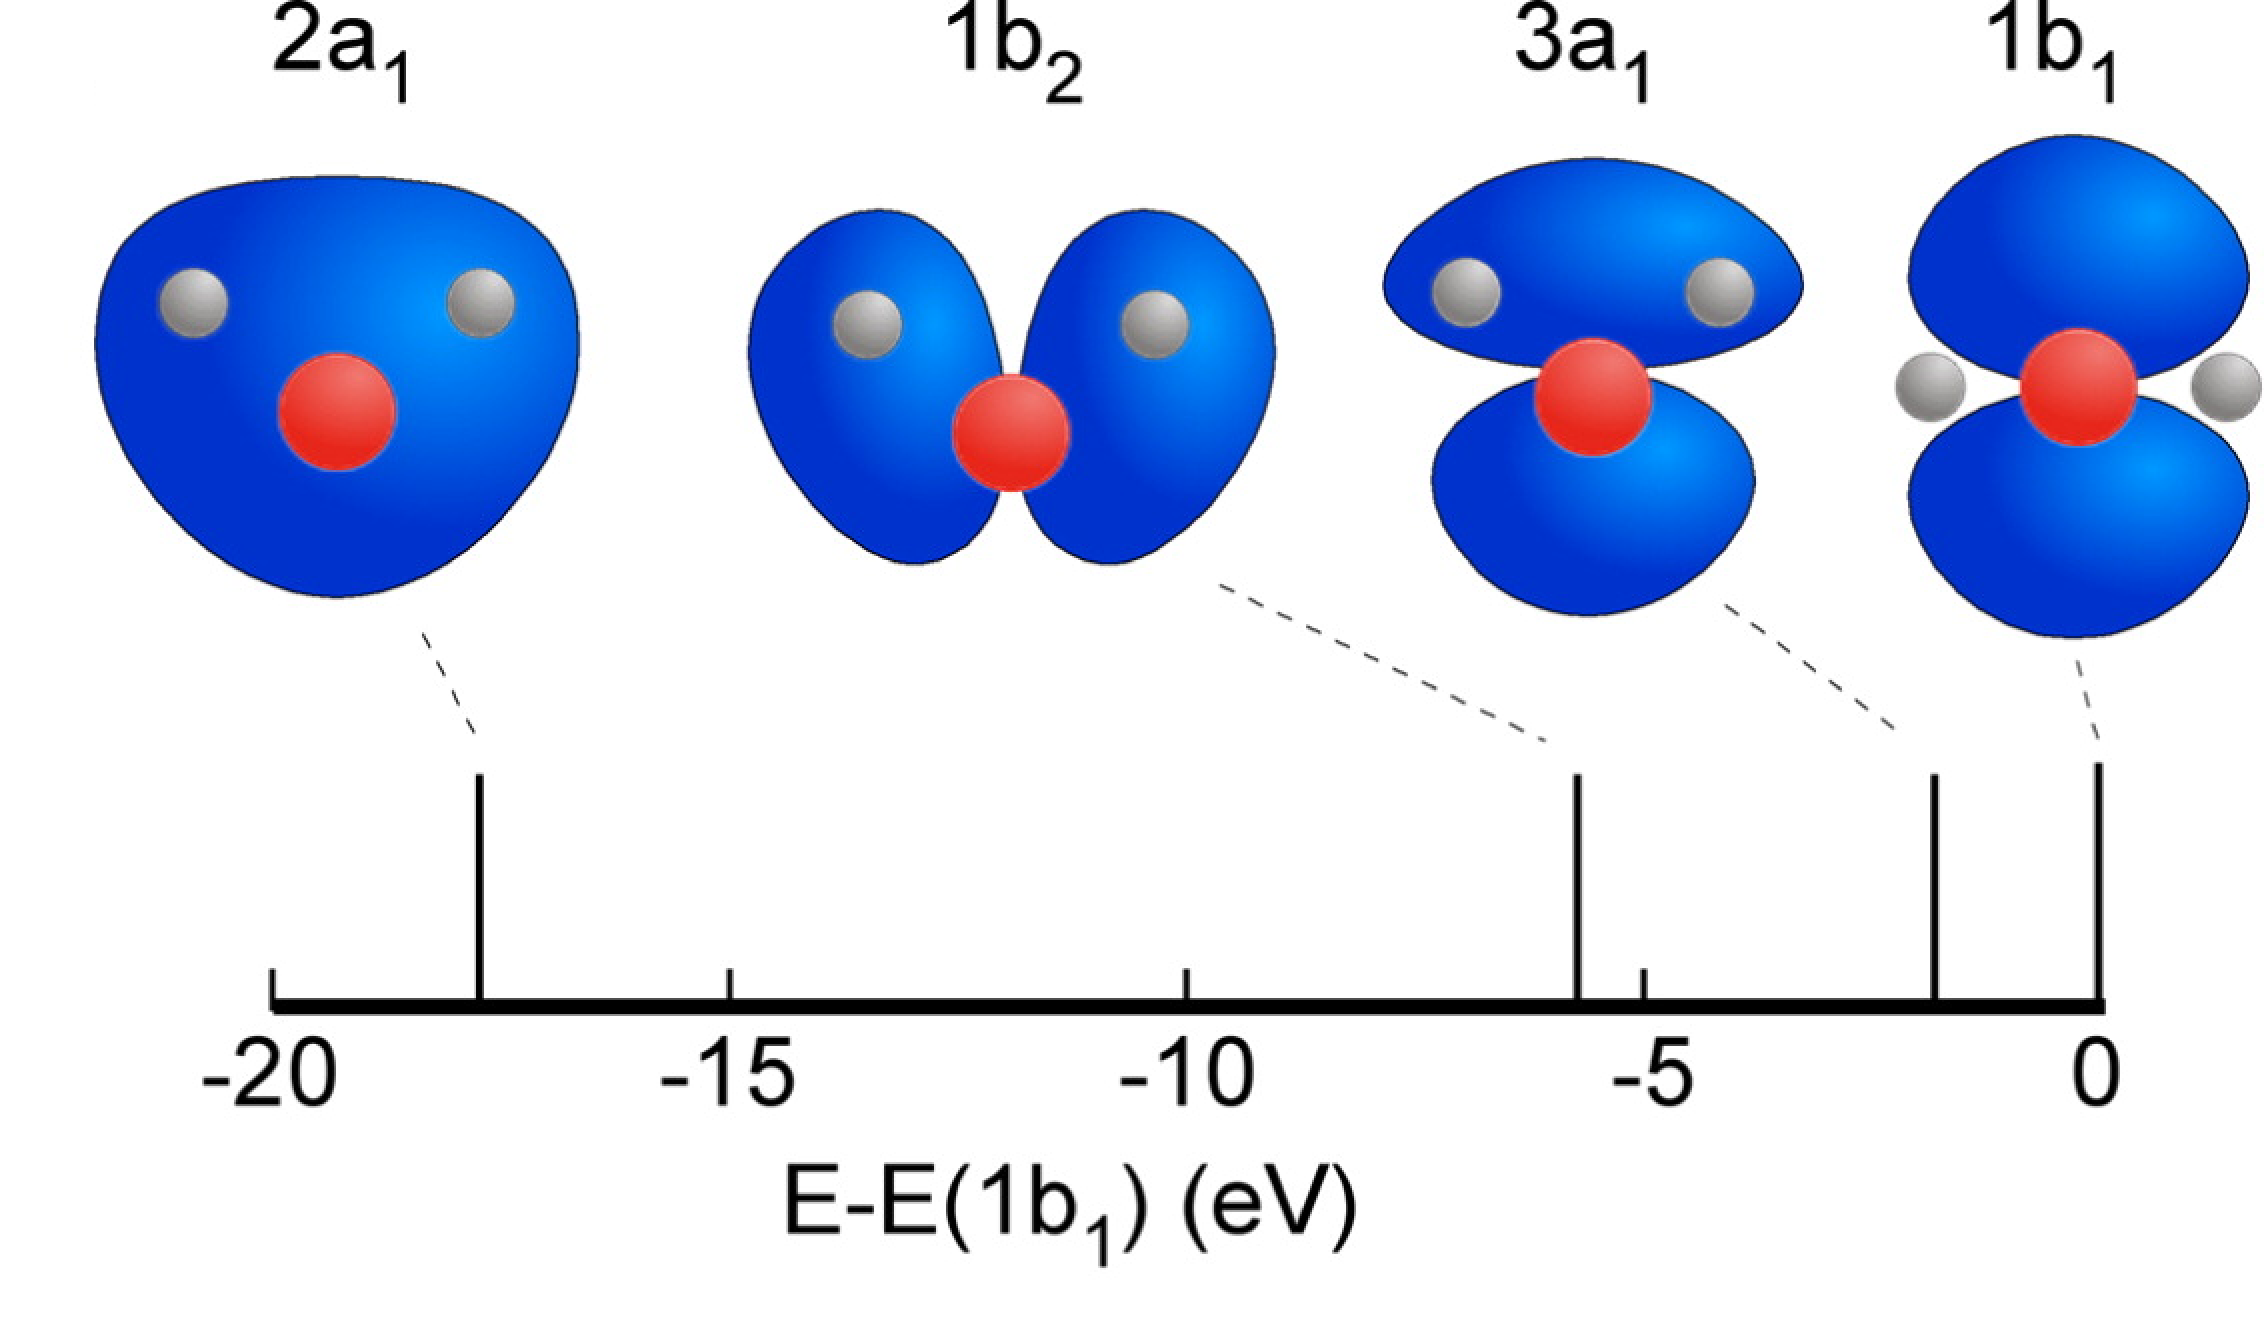
\includegraphics[width=\textwidth]{figs/orbital_water.png}
		\legend{Fonte: \citeauthor{Michaelides2006}}
		\label{fig:orbital-wat}
	\end{subfigure}\,
	\begin{subfigure}{0.57\textwidth}
		\caption{\textit{Monômero adsorvido}}
		\centering
		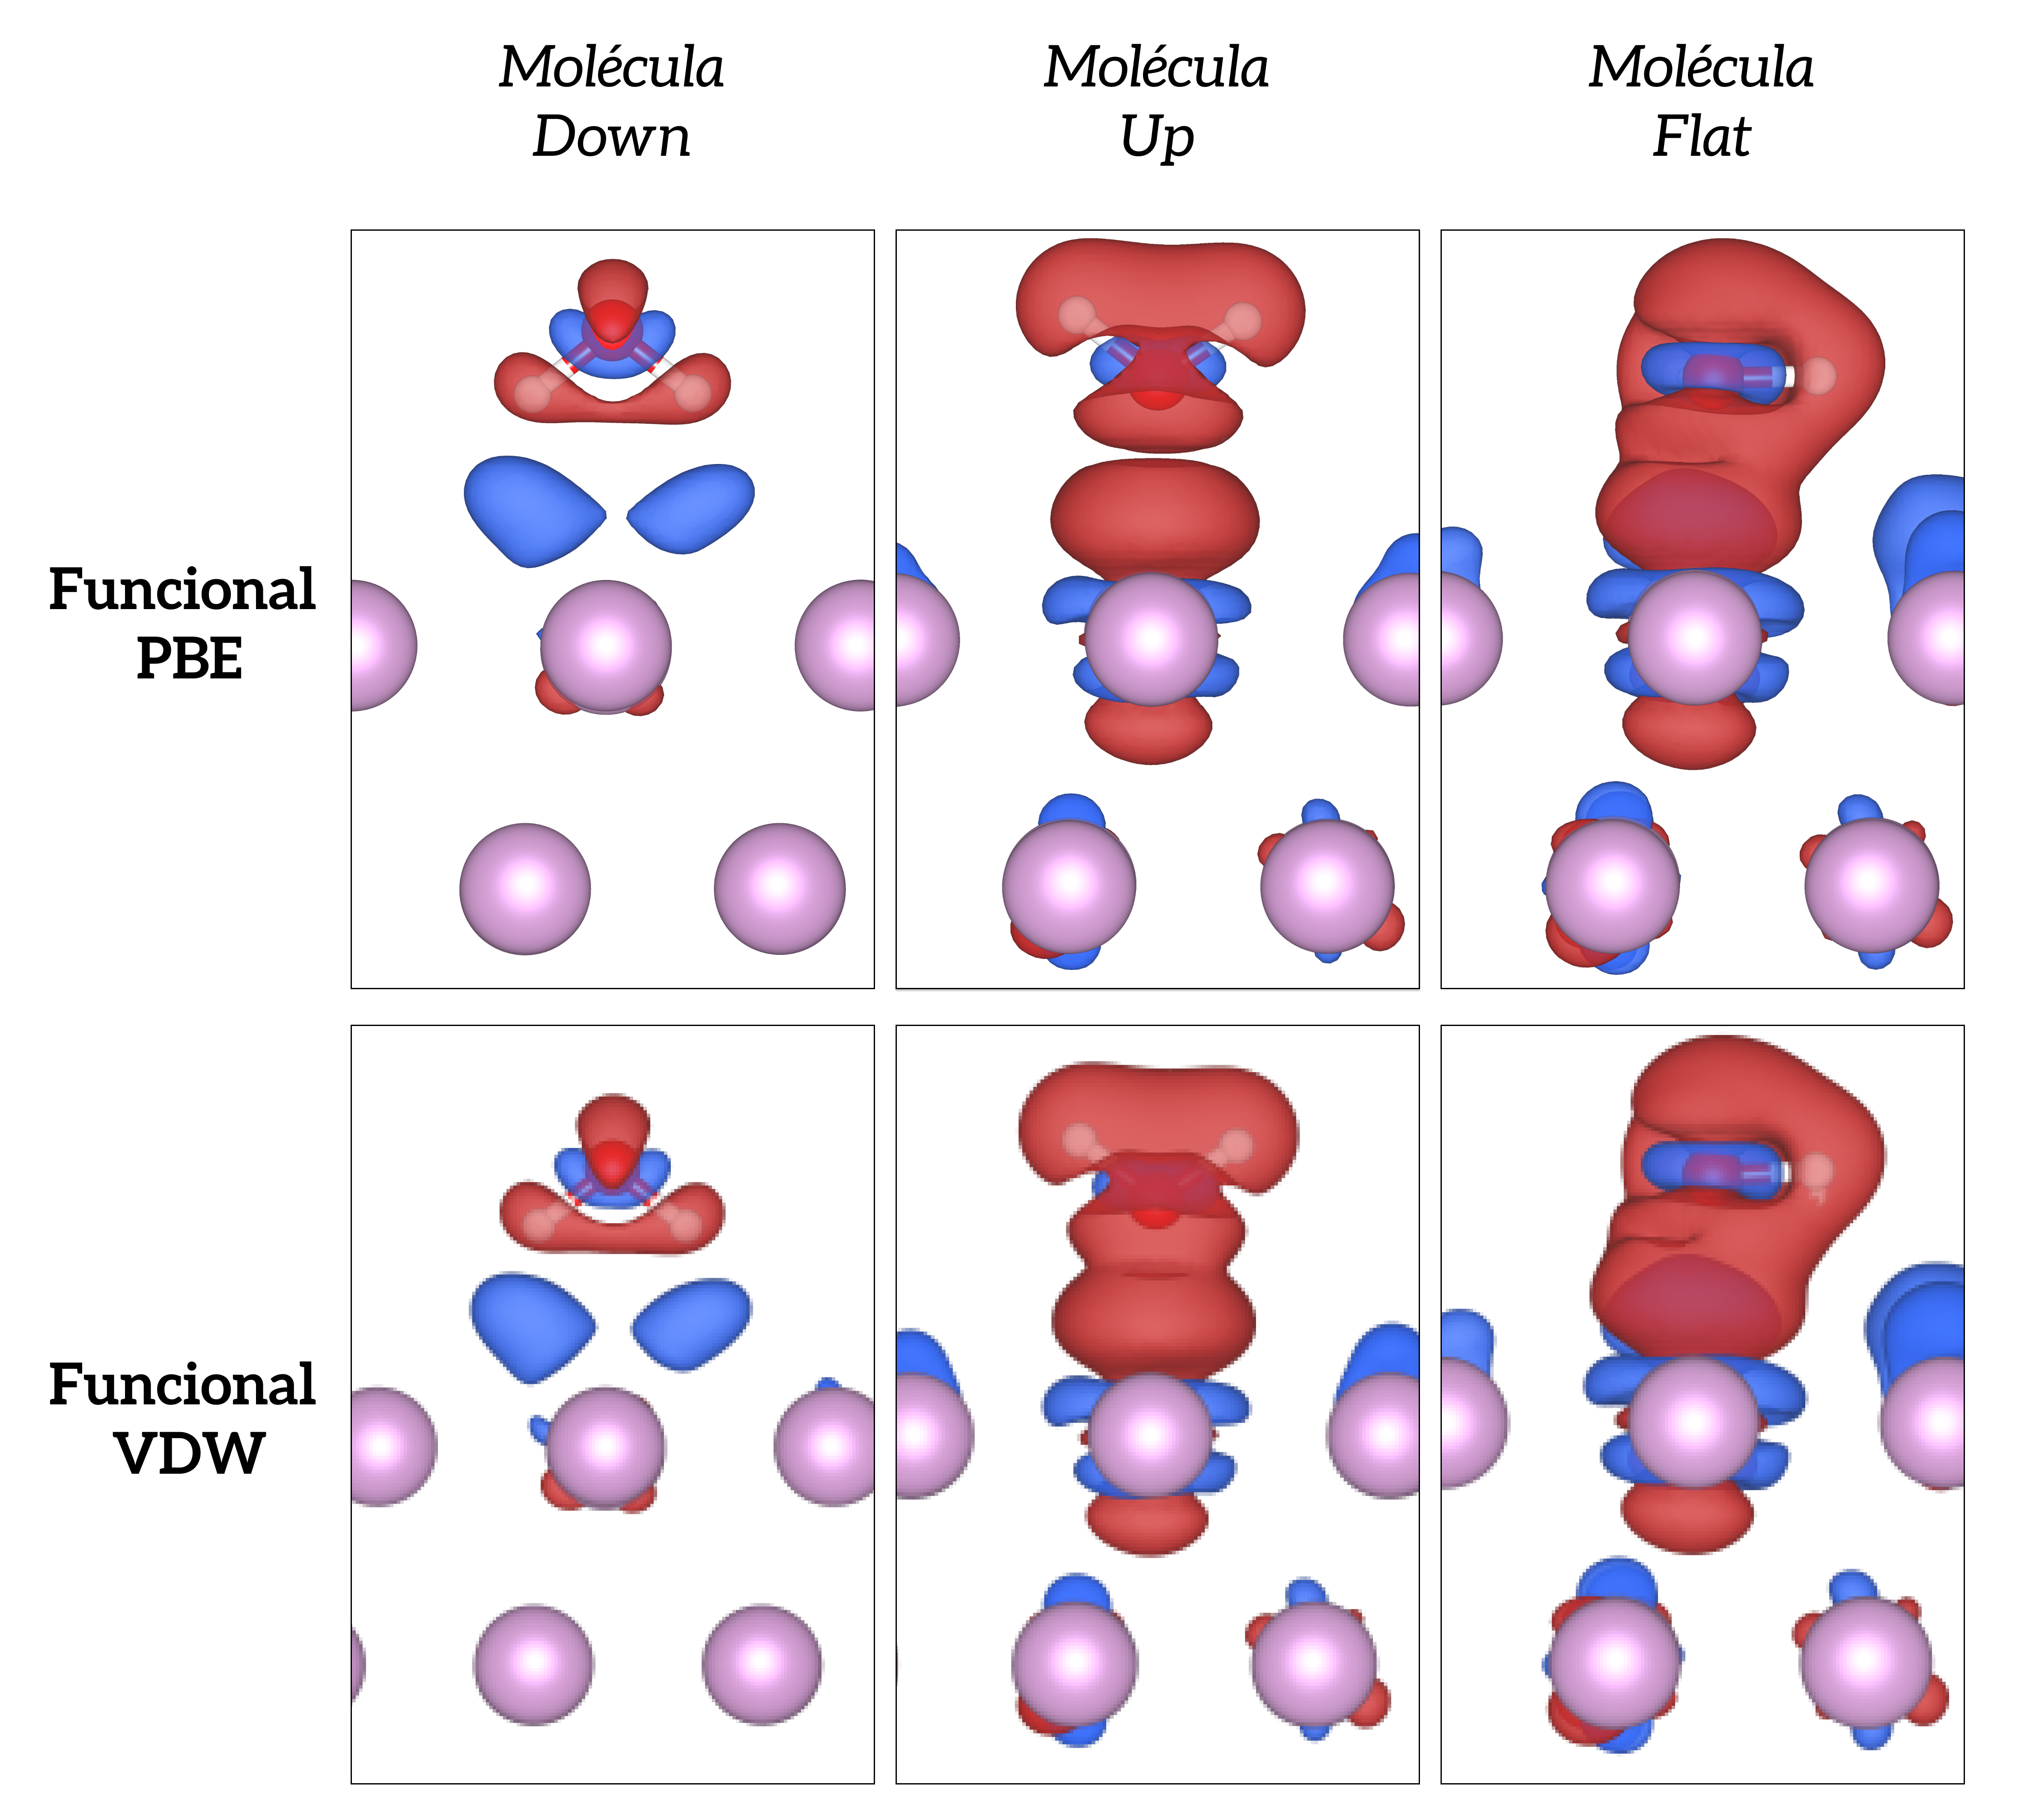
\includegraphics[width=\textwidth]{figs/graph_densidade.png}
		\legend{Fonte: compilação da autora.}
		\label{fig:dens-monomer}
	\end{subfigure}
\end{figure}

Com o intuito de investigar a natureza da interação entre a água e o metal, bem como explicar a maior estabilidade da orientação \textit{flat} em relação as demais, analisamos as diferenças de densidade de carga ($\Delta\rho$). A análise da estrutura eletrônica através do $\Delta\rho$ permite visualizar e associar os orbitais envolvidos na interação entre a molécula de água e a superfície metálica para cada orientação. Isso foi feito para o monômero adsorvido na superfície de tamanho $6\times4\times4$ descrito pelos funcionais PBE e VDW-BH (Figura \ref{fig:dens-monomer}). Analisando as densidades do monômero adsorvido e comparando com os mais altos orbitais moleculares ocupados da molécula de água isolada (Fig. \ref{fig:orbital-wat}), vemos que a orientação \textit{up} favorece a interação com o metal através do orbital $3a_1$, ao passo que a orientação \textit{flat} favorece a interação com o orbital $1b_1$.  No entanto, considerando que em metais platinados o orbital $b_1$ está mais próximo ao nível de Fermi, então a orientação \textit{flat} diminui a repulsão entre os pares solitários do átomo de oxigênio com o orbital d do metal e estabiliza a adsorção \cite{michaedelis,monomer}.
\begin{table}[b!]
	\centering	\caption{Valores da energia de adsorção $ E_{ads}(\si{eV}) $ obtido para cada orientação do monômero, bem como a diferença da energia total $ \Delta E $ em relação à energia da orientação flat. Na tabela estão apresentados as energias calculadas com $ 4\times4\times4 $ pontos k.\label{tab:energies}}
	\begin{tabular}{cccccccccccc} 
		\hline\hline\addlinespace[3.8pt]
		\multicolumn{12}{c}{\textbf{Diferenças de Energias do Sistema Completo $ \Delta E$ (eV)}}                                                                                                                                              \\ 
		\midrule
		\multirow{3}{*}{} & \multicolumn{5}{c}{PBE}                                                          &  & \multicolumn{5}{c}{VDW-BH}                                                           \\ 
		\cmidrule{2-6}\cmidrule{8-12}
		& \multicolumn{2}{c}{$4\times4\times4$} &  & \multicolumn{2}{c}{$6\times4\times4$} &  & \multicolumn{2}{c}{$4\times4\times4$} &  & \multicolumn{2}{c}{$6\times4\times4$}  \\ 
		\cmidrule{2-3}\cmidrule{5-6}\cmidrule{8-9}\cmidrule{11-12}
		& E$_{ads}$ & $\Delta$E                 &  & E$_{ads}$ & $\Delta$E                 &  & E$_{ads}$ & $\Delta$E                 &  & E$_{ads}$ & $\Delta$E                  \\ 
		\midrule
		\textbf{Flat}              & 0.25      & -                         &  & 0.27      & -                         &  & 0.44     & -                         &  & 0.45      & -                          \\ 
		
		\textbf{Up}                & 0.16      &         -0.13             &  & 0.18      &       -0.13               &  & 0.34     &             -0.15         &  & 0.35      &     -0.14                  \\ 
		
		\textbf{Down}              & 0.10      &          -0.16            &  & 0.10      &         -0.18            &  & 0.21     &         -0.23             &  & 0.21      &      -0.24                 \\ 
		\hline\hline
	\end{tabular}
	\legend{Fonte: Compilação da autora.}
\end{table}

Os gráficos de diferenças de carga mostram que a interação água/metal ocorre por meio da interação dos orbitais mais altos da molécula de água com os orbitais \textit{d} do metal. Como essa interação é similar à uma ligação de hidrogênio (\textit{pseudo H-bond}), na qual o metal age como uma segunda molécula de água, então transferência de carga vai depender da orientação do monômero, bem como de qual espécie está agindo como doadora ou receptora. Em relação às orientações \textit{up} e \textit{flat}, o metal age como ``doador'' e a molécula como receptora e observa-se uma polarização na região entre o metal e a molécula. Essa polarização provoca um enfraquecimento da molécula de água, como observado pelo alongamento da ligação O-H na molécula \textit{flat} e pelo aumento do ângulo $\Theta$ na molécula \textit{up}. No caso da molécula \textit{down}, a polarização é menor e o metal age como ``receptor". Isso é visto pela diminuição da densidade de carga na região dos hidrogênios e um aumento da densidade na superfície metálica. 

%Além disso, é possível comparar o efeito da força de dispersão na transferência de carga por meio da flutuação de densidade de carga $ \Omega\rho $ entre os dois funcionais. Assim, o funcional VDW-BH é mais sensível à transferência de carga, uma vez que apresenta maiores variações na densidade de carga que o funcional PBE.

Uma vez definido que a orientação \textit{flat} é a mais estável, investigamos a estabilidade das demais orientações através das diferenças de energias ($ \Delta E$). Para isso, subtraímos a energia do sistema completo da molécula \textit{flat} com a energia das demais orientações -- Tabela \ref{tab:energies}. Para computar essa diferença utilizamos a energia do sistema completo calculado com $ 4\times4\times4 $ pontos k. Os valores de $ \Delta E $ junto com os gráficos de $ \Delta\rho $ mostram que a orientação \textit{up} é mais estável que a orientação \textit{down}, uma vez que os valores de energia são mais próximos à orientação \textit{flat}. Dessa forma, após caracterizar o efeito da adsorção no metal nas propriedades geométricas e eletrônicas, bem como determinar a estabilidade das estruturas, analisaremos o efeito nas propriedades vibracionais do sistema.


\subsection*{Modos normais de vibração}
 Os modos normais de vibrações são utilizados para obter informações intramoleculares, além de interações intermoleculares, tais como ligações de hidrogênio entre moléculas de água e interações entre a água e o metal. Isso ocorre devida à alta correlação entre as forças de ligação de hidrogênio e as frequências de vibração de estiramento - ligaçao O-H. Assim, uma alta frequência do modo de estiramento indica uma fraca interação intermolecular da ligação de hidrogênio e consequentemente, ligaçoes O-H mais fortes \cite{modos}. 

 Para uma molécula de água, os três modos normais de vibração fundamentais são deformação angular tesoura (\textit{bending}) e estiramento simétrico (\textit{symmetric stretching}) e assimétrico (\textit{asymetric stretching}), ilustrados na Figura \ref{fig:vibra}. O primeiro modo de vibração corresponde à expansão e compressão do ângulo entre os átomos de H ($ \Theta $). Os modos de vibração \textit{stretching} correspondem às vibrações realizadas entre as ligaçoes O-H, onde no modo simétrico as duas ligaçoes O-H alongam e se contraem simultaneamente no mesmo sentido e no modo assimétrico as vibrações ocorrem alternadamente.
 
 \begin{figure}[H]
	\centering
	\caption{Ilustração esquemática mostrando os modos de vibração do monômero\label{fig:vibra}}
	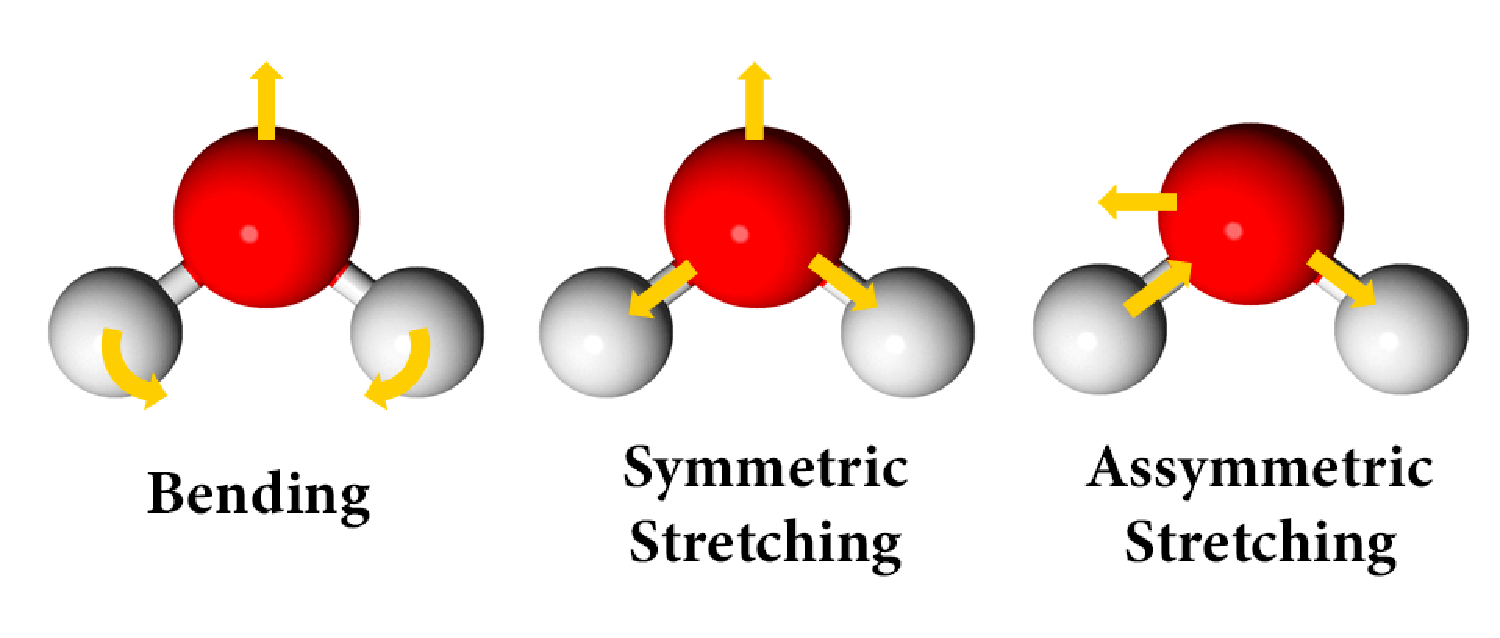
\includegraphics[scale=0.32]{figs/setas.pdf}
	\legend{Fonte: Compilação da autora.}
\end{figure}
 
\begin{table}[b!]
 	\centering
 	\caption{Tabela contendo as frequências ($ \si{cm}^{-1} $) dos modos normais do monômero isolado, computacional e experimental, e das moléculas adsorvidas no Pd em diferentes orientações. \label{tab:modos}}
 	\begin{threeparttable}
 		\begin{tabular}{ccccccccc} 
 			\hline\hline\addlinespace[3.6pt]
 			\multicolumn{9}{c}{\textbf{Frequências dos Modos Normais (\si{\cm}$ ^{-1} $) - Monômero}}                                                                                                                            \\ 
 			\midrule
 			\multirow{3}{*}{}              & \multicolumn{2}{c}{Bending}              &  & \multicolumn{2}{c}{\textit{Stretching} (S)}                &  & \multicolumn{2}{c}{\textit{Stretching} (AS)}               \\ 
 			\cmidrule{2-3}\cmidrule{5-6}\cmidrule{8-9}&PBE & VDW-BH &  & PBE &VDW-BH&  & PBE &VDW-BH \\ 
 			\midrule Flat   & 1621& 1606             &  & 3651              &3599             &  &3741            & 3694              \\ 
 			Up & 1641& 1645  &  & 3768              & 3719              &  & 3879              & 3842               \\		
 			Down & 1590             &
 			1562           &  & 3624              & 3565   &  & 3694              & 3637               \\				 H$ _2$O Isolado  & 1672             &1665
 			&  & 3692             &  3641  &  & 3791             &   3745           \\ \midrule
 			H$ _2 $O Isolado Exp.\tnote{$\dagger$} & \multicolumn{2}{c}{1596.9}                         &  & \multicolumn{2}{c}{3632.5}                   &  & \multicolumn{2}{c}{3725.7}                       \\ \hline\hline
 		\end{tabular}
 		\begin{tablenotes}\footnotesize
 			\item[$\dagger$] \citeauthor{ref-modos}
 		\end{tablenotes}
 	\end{threeparttable}
 	\legend{Fonte: compilação da autora.}
 \end{table}
 
 Dessa forma, com o intuito de analisar as alterações nas propriedades vibracionais que a adsorção no metal provoca nos modos normais de um monômero, calculamos as frequências de vibração para cada orientação e em seguida comparamos aos valores experimentais e teóricos do monômero isolado (Tabela \ref{tab:modos}).
 
 As frequências obtidas via simulações computacionais com o funcional VDW-BH para o monômero isolado foram as que mais se aproximaram dos valores experimentais obtidos por meio de espectroscopia de infravermelho \cite{ref-modos}. Para o modo de vibração \textit{bending} as vibrações diferem entre $ 4\% $ e $ 5\%$ do valor experimental para os funcionais VDW-BH e PBE, respectivamente; em relação às frequências de \textit{stretching} simétrico e antisimétrico as variações são 1.6 e $1.8\% $ para o funcional PBE e 0.2 e $0.5\% $ para o funcional VDW-BH, respectivamente. 

 Para as estruturas adsorvidas foi usado como parâmetro de comparação os valores do monômero isolado obtido via simulações. Assim, para o modo \textit{bending} observa-se a maior diminuição (deslocamento para o vermelho - \textit{redshift}) para a orientação \textit{down}, $ \delta_{PBE}\sim 80 \,\si{\cm}^{-1}$ e $ \delta_{VDW-BH}\sim 100 \,\si{cm}^{-1}$. As configurações \textit{up} tiveram os menores \textit{redshift} na frequência de \textit{bending}: entre $ 20 $ e $ 30 \,\si{cm}^{-1}$ para os funcionais PBE e VDW-BH, respectivamente.

Em relação às frequências de \textit{stretching}, houve um aumento entre $ \sim 80 \,\si{cm}^{-1}$ e $ \sim 100 \,\si{cm}^{-1}$ nas frequências da orientação \textit{up}. Esse aumento decorre do fato de que nessa orientação não há interação entre os átomos de hidrogênio e a superfície metálica, logo essas frequências descrevem uma molécula mais covalente e com ligações O-H mais fortes. Por outro lado, os menores valores de frequências correspondem às estruturas \textit{down} com diminuições entre $ \sim 80 \,\si{cm}^{-1}$ e $ \sim 110 \,\si{cm}^{-1}$. Isso ocorre devido à interação da molécula com a superfície metálica e indica uma interação mais intensa. Para a molécula \textit{flat} as diminuições nas frequências foram entre $40$ e $ 60 \,\si{cm}^{-1} $. Esse comportamento de \textit{redshift} revela como a adsorção no metal modifica significativamente a ligação covalente O-H da molécula de água. 

 Por fim, comparando os valores obtidos entre o funcional PBE e VDW-BH, observa-se que o funcional VDW-BH fornece valores menores, particularmente para os modos de \textit{stretching}. Assim, com o funcional VDW-BH as moléculas de água se tornam menos covalentes e se ligam mais fortemente ao metal, fazendo com que as frequências de \textit{stretching} diminuam \cite{adrien}.  
%Modos Normais - Monômero 

Nessa seção revisitamos o problema da adsorção do monômero em superfícies metálica com o intuito de caracterizar a interface água metal, uma vez que esse problema motivou diversas investigações teóricas e experimentais ao longo dos últimos anos \cite{salmeron,monomerexp1, monomerexp2,michaedelis,monomer,adrien,review_new}. Do ponto de vista experimental, a adsorção da água em vários metais foi estudada utilizando-se especialmente Microscopia de Tunelamento com Varredura (\textit{Scanning tunneling microscopy} - STM) \cite{salmeron,monomerexp1,monomerexp2}. Todavia, essas caracterizações são dificultadas pela tendência das moléculas de água de se agruparem em clusters e pelo fato de que técnicas de STM não são suficientemente sensíveis para revelar a estrutura interna de moléculas adsorvidas \cite{michaedelis}. Por outro lado, no âmbito da eletrostática a orientação que favorece a interação com o metal é a molécula perpendicular à superfície \cite{adrien}. Nessa perspectiva, o uso de simulações computacionais permitiu esclarecer tais questões ao revelar que a molécula adsorve paralelamente e diretamente acima do átomo metálico (sítio \textit{atop}).

Assim, nossos resultados corroboram com os achados da literatura e mostram que a estrutura \textit{flat} é a mais estável seguida da orientação \textit{up}. Além disso, os resultados revelaram que o funcional VDW-BH intensifica a ligação da molécula de água com o metal. Como resultado, as energias de adsorção aumentam e as frequências de \textit{stretching} diminuem. Em relação às características estruturais do sistema, temos que a célula unitária de tamanho $ 6\times4\times4 $ descreve melhor a geometria do sistema, uma vez que diminui interações fictícias, ao passo que a convergência da energia é atingida com $ 2\times2 $ pontos k. Por fim, através de análises da estrutura eletrônica e de caracterizações estruturais e vibracionais, vimos como a adsorção no metal afeta a molécula de água. Essas caracterizações serão complementadas no capítulo seguinte ao investigar como essas propriedades são alteradas pela aplicação de um potencial externo. Além disso, na seção seguinte completaremos a caracterização da interface água/metal ao analisar como as ligações de hidrogênio são afetadas pela presença da superfície metálica através da adsorção de uma camada de água. No capítulo \ref{cap:bias}

\section{Camada de Água adsorvida no Pd(111)\label{sec:re-la}}
\subsection*{Propriedades estruturais e eletrônicas}
Após caracterizar as interações e as propriedades geométricas e vibracionais do monômero adsorvido, essas análises foram estendidas para camadas de água bidimensionais de tamanhos $ (\sqrt{3}\times\sqrt{3})R30\si{\degree} $ (\textit{bilayers}) adsorvidas sobre uma superfície metálica de Pd. A estrutura dessa camada é similar aos planos (0001) e (111) do gelo \textit{bulk}, no qual cada molécula de água forma 3 ligações de hidrogênio e estão arranjadas em hexágonos de tamanhos proporcionais ao parâmetro de rede do metal. Nesse modelo, metade das moléculas de água estão na orientação \textit{flat} e diretamente ligadas ao metal, além de atuarem como doadoras em ligações de hidrogênio com as moléculas adjacentes. A outra metade das moléculas não está diretamente ligada ao metal e forma três ligações de hidrogênio com as moléculas adjacentes - duas ligações atuando como receptor e uma como doador. Assim, as moléculas com orientações \textit{flat} estão em distâncias $ d_{OM} $ diferentes das demais moléculas. Esses modelos foram baseados em resultados experimentais de STM, nos quais foram observadas estruturas de clusters de água hexagonais em diversos metais, em especial no Pd(111) (Figura \ref{fig:layer_stm})  \cite{layer_dft,review,review2,review_new}

\begin{figure}[H]
	\centering
	\caption{(a) Imagens de clusters de $ D_2O $ adsorvidos no Pd(111) a 100K obtidas via STM ($ 175\times135\,\si{\angstrom} $); (b) ampliação de $ 41\times53\,\si{\angstrom} $ e (c) ampliação $ 20\times20\,\si{\angstrom} $.}
	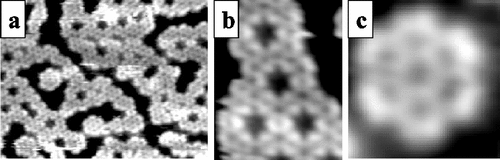
\includegraphics[scale=0.7]{figs/layer_stm.png}
	\legend{Fonte: \citeauthor{layer_dft}}
	\label{fig:layer_stm}
\end{figure}  

A partir dos arranjos hexagonais observados nos experimentos de STM os modelos de camada bidimensional propostos sugerem que metade das moléculas estejam nas configurações \textit{flat} e as demais nas configurações \textit{flat-down} (camada \textit{H-down}) ou nas orientações \textit{flat-up} (camada \textit{H-up}) -- representadas na Figura \ref{fig:complete}. Além disso, os modelos consideram que as camadas podem ser formadas por uma mistura das orientações descritas acima (Fig. \ref{fig:complete}c) ou também apresentar moléculas dissociadas \cite{layer_dft}. Assim, nessa seção analisamos o efeito da adsorção no metal nas ligações de hidrogênio através das propriedades das camadas \textit{H-down}, \textit{H-Up} e \textit{H-Down/Up}.

\begin{figure}[b!]
	\centering
	\caption{Representação das três camadas de água do tipo bilayer utilizadas nas simulações computacionais. }
	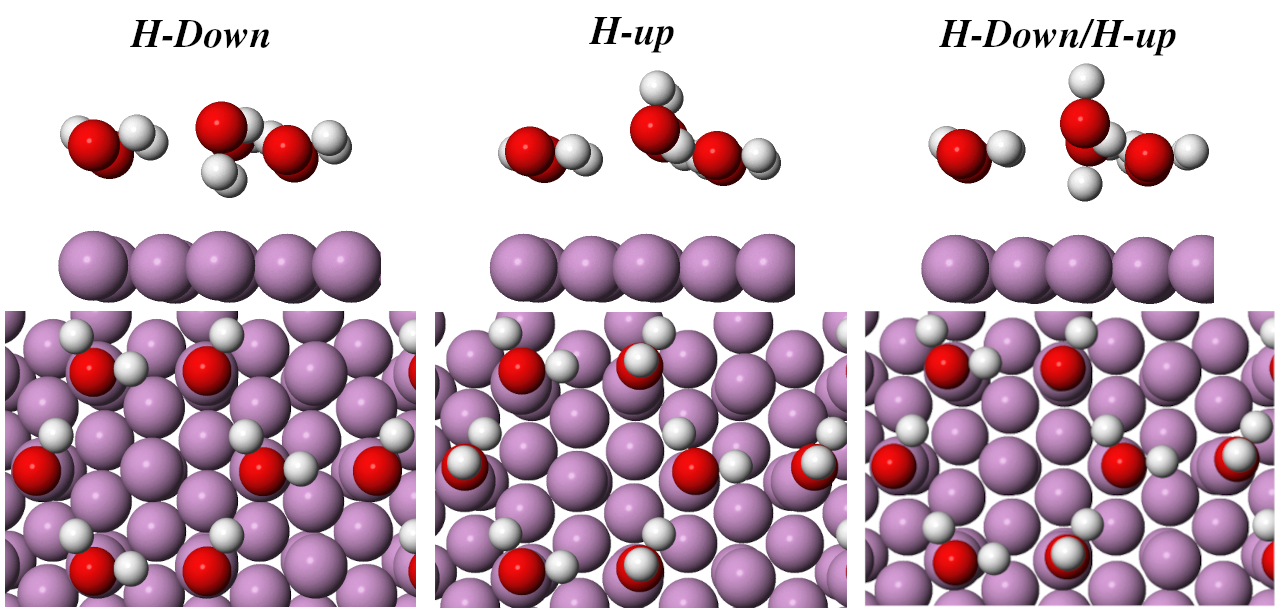
\includegraphics[scale=0.3]{figs/complete2.png}
	\legend{Fonte: Compilação da autora.}
	\label{fig:complete}
\end{figure}  

Para descrever as camadas utilizamos células unitárias com 16 moléculas de água adsorvidas sobre uma superfície de Pd de tamanho $ 6\times4\times4 $. Escolhemos esse tamanho de superfície pois, de acordo com os resultados do monômero, essa superfície apresentou melhores resultados. Além disso, considerando a convergência do monômero adsorvido a partir de $2\times2$ pontos k, calculamos as energias de adsorção das camadas de acordo com os esquemas de pontos k: $1\times1$ e $2\times2$. Durante a otimização os átomos metálicos eram mantidos fixos e as moléculas de água eram relaxadas. Para cada esquema calculamos a energia considerando também correção dos erros de superposição de bases (BSSE). Os funcionais de troca e correlação utilizados foram PBE e VDW-BH.

As propriedades geométricas analisadas foram obtidas a partir da média sobre as distâncias entre os átomos de oxigênio (${d_{OO}}$), entre os átomos de oxigênio e de paládio (${d_{OM}}$) e entre os átomos de hidrogênio e oxigênio (${d_{OH_1}}$ e ${d_{OH_2}}$) para cada uma das moléculas que compõem as camadas e suas respectivas orientações \textit{flat}, \textit{flat-down} e \textit{flat-up} (Figura \ref{fig:geometric}). Em relação à definição de qual átomo de hidrogênio corresponde a $H_1$ ou $H_2$, adotou-se a convenção de que nas orientações \textit{flat-up} e \textit{down} o átomo que faz ligação de hidrogênio é $H_1$ e o que está ``livre'' é denominada $H_2$. 


\begin{figure}[H]
	\centering
	\caption{Distâncias interatômicas analisadas na camada de água adsorvida no Pd.} 
	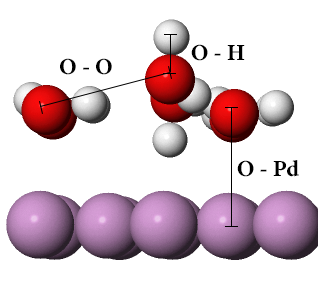
\includegraphics[scale=0.43]{figs/geometric.png}
	\legend{Fonte: Compilação da autora.}
	\label{fig:geometric}
\end{figure}

 
Diferentemente do monômero adsorvido, a definição da energia de adsorção da camada não é tão direta. Isso ocorre pela dificuldade em separar as diferentes contribuições para a energia. Assim, adotando as definições apresentadas por \citeauthor{adrien}, a energia de adsorção da camada ($ E_{ads} $) é definida como a energia média por molécula de água:
\begin{equation}
	E^{bilayer}_{ads}=-\frac{1}{n}\pqty{E_{all}-E^{bilayer}_{H_2O}- E_{metal}}
\end{equation}
onde $ n $ é o número de moléculas de água na célula unitária, $ E_{all} $ é a energia do sistema com a camada adsorvida, $ E_{metal} $ e $ E^{bilayer}_{H_2O} $ são as energias da superfície metálica e da camada de água calculados com a configuração atômica da camada, respectivamente. Essa energia representa o ganho de energia ao mover a camada de água do infinito à superfície de Pd.

Outra definição apresentada na literatura \cite{adrien} é a de energia de coesão, que corresponde à energia necessária para criar uma camada bidimensional de gelo acima da superfície de Pd(111):

\begin{equation}\label{eq:coesao}
	E_{coesão/H_2O}=\frac{1}{n}\pqty{E_{all}-n\cdot E_{isolated}-E_{metal}}
\end{equation}
onde nesse caso, $E_{isolated}$ é a energia de um monômero isolado, multiplicado pelo número de moléculas $n$. Normalmente, os resultados reportados na literatura \cite{adrien,layer} correspondem à energia de coesão.

%DOADOR É O $H_2$.

Como foi dito anteriormente, quando aumentamos a complexidade do sistema e passamos de um monômero adsorvido para uma camada aumentamos também a complexidade das interações. Nesse sentido, para analisar o efeito da adsorção no metal sobre as ligações de hidrogênio, faremos a comparação das propriedades analisadas com as do dímero no vácuo. Isso se dá pelo fato de esse sistema é um protótipo da ligação de hidrogênio, logo a comparação das propriedades da camada de água adsorvida em relação às do dímero no vácuo revela o efeito do metal sobre as ligações de hidrogênio e detalhes a interação água/metal \cite{monomer}.
\begin{table}[b!]
	\centering
	\caption{Tabela com as energia de ligação (eV) e as distâncias entre os átomos de oxigênio $d_{OO}$ ($\si{\angstrom}$) e entre os átomos de hidrogênio e oxigênio $d_{OH}$ ($\si{\angstrom}$) do dímero de água no vácuo calculadas com os funcionais PBE e VDW-BH, bem como o valor experimental. Nos dois casos, o valor $d_{OH}=0.98\,\si{\angstrom}$ correspondem à ligação O-H doadora na ligação de hidrogênio. \label{tab:dimero}}
	\begin{threeparttable}
		\begin{tabular}{ccccccc} 
			\hline\hline
			\multicolumn{7}{c}{ \textbf{Dímero no Vácuo} }        \\ \midrule
			&  & Energia ($ \si{\eV} $)                                  &  & $ d_{OO}(\si{\angstrom})$                                         &  & $ d_{OH}(\si{\angstrom})$                \\\midrule
			PBE    &  & 0.26                                   &  & 2.90                                         &  & 0.97/0.98                              \\
			VDW-BH &  & 0.24                                   &  & 2.91                                         &  & 0.97/0.98                              \\
			Exp.\tnote{$\dagger$}   &  & 0.23                                   &  & 2.98                                         &  &  -                                      \\
			\hline\hline
		\end{tabular}
		\begin{tablenotes}\footnotesize
			\item[$\dagger$] \citeauthor{dimer-exp}
		\end{tablenotes}
	\end{threeparttable}
\end{table}
\begin{table}[t!]
	\centering
	\caption{Propriedades geométricas das camadas de água H-Down, H-Up e H-Down/Up. Após os átomos atingirem as posições de mínimo, foi medido para cada camada a distância média entre os átomos de oxigênio ($ {d_{OO}} $). Considerando as diversas orientações das moléculas que compões as camadas, foi medido para cada tipo de orientação a distância média entre o átomo de O e de Pd ($ {d_{OM}} $) e as distâncias médias entre o oxigênio e os átomos de hidrogênio ($ {d_{OH_1}}$ e $ {d_{OH_2}}$).\label{tab:camada}}
	\begin{tabular}{cccccccccccc} 
		\hline\hline\addlinespace[3.5pt]
		\multicolumn{12}{c}{\textbf{Propriedades Geométricas ($ \si{\angstrom} $) - Camada de Água}}                                                                                                                                                                                                              \\ 
		\midrule
		\multicolumn{3}{c}{\multirow{2}{*}{\textbf{Camada}}}                                                                                                  &  & \multicolumn{2}{c}{\textbf{H-Down}} &  & \multicolumn{2}{c}{\textbf{H-Up}} &  & \multicolumn{2}{c}{\textbf{H-Down/Up}}  \\ 
		\cmidrule{5-6}\cmidrule{8-9}\cmidrule{11-12}
		\multicolumn{3}{c}{}                                                                                                                                  &  & PBE  & VDW                      &  & PBE  & VDW                     &  & PBE  & VDW                             \\ 
		\midrule
		&                                                                                       & ${d_{OO}}$   &  & 2.84 & 2.81                         &  & 2.86 & 2.83                       &  & 2.87 & 2.83                               \\ 
		\midrule
		\multirow{9}{*}{\textit{Moléculas}} & \multirow{3}{*}{\textit{Flat}}                                                        & ${d_{OM}} $ &  & 2.66 & 2.50                         &  & 2.68 & 2.52                       &  & 2.59 & 2.46                               \\
		&                                                                                       & ${d_{OH_1}}$ &  & 0.99 & 1.00                         &  & 0.99 & 0.99                       &  & 0.99 & 0.99                               \\
		&                                                                                       & ${d_{OH_2}}$  &  & 0.99 & 1.00                         &  & 0.99 & 0.99                       &  & 0.99 & 0.99                               \\ 
		\cmidrule{2-12}
		& \multirow{3}{*}{\begin{tabular}[c]{@{}c@{}}\textit{Flat}\\\textit{Down}\end{tabular}} & ${d_{OM}} $ &  & 3.06 & 2.99                         &  & -    & -                          &  & 3.05 & 2.99                               \\
		&                                                                                       & ${d_{OH_1}}$  &  & 0.99& 1.00                         &  & -    & -                          &  & 0.99 & 1.00                               \\ 
		&                                                                                       & ${d_{OH_2}}$  &  & 1.00 & 1.01                         &  & -    & -                          &  & 1.00 & 1.02                               \\
		\cmidrule{2-12}
		& \multirow{3}{*}{\begin{tabular}[c]{@{}c@{}}\textit{Flat}\\\textit{Up}\end{tabular}}   & ${d_{OM}} $ &  & -    & -                            &  & 3.20 & 3.08                       &  & 3.29 & 3.15                               \\
		&                                                                                       & ${d_{OH_1}}$ &  & -    & -                            &  & 1.00 & 1.00                      &  & 1.00 & 1.00                               \\
		&                                                                                       & ${d_{OH_2}}$ &  & -    & -                            &  & 0.97 & 0.97                       &  & 0.97 & 0.97                               \\
		\hline\hline
	\end{tabular}	
	\legend{Fonte: compilação da autora.}
\end{table}

Para tanto, iniciamos os cálculos eletrônicos com dímero no vácuo e analisamos as distâncias entre os átomos de Oxigênio ($d_{OO}$) e a a energia de ligação -- Tabela \ref{tab:dimero}. O funcional VDW-BH forneceu a energia (0.24 eV) mais próxima ao experimental (0.23 eV) e as distâncias $ d_{OO} $ estão de acordo com o experimental \cite{dimer-exp}. Considerando a camada de água adsorvida no metal (Tabela \ref{tab:camada}), observa-se que as distâncias $ d_{OO} $ diminuem em relação ao dímero no vácuo devido à presença do metal. Em especial, essa redução é maior para os resultados obtidos com o funcional VDW-BH nas três camadas, $2.81\;\AA$ e $2.83\;\AA$ comparados com $2.91\;\AA$ do dímero no vácuo. Além disso, observa-se que a camada H-Down apresenta as menores distâncias $d_{OO}$, portanto, do ponto de vista estrutural essa camada possui a ligação de hidrogênio mais intensa e mais estável. Portanto, a adsorção no metal diminui as distâncias entre as moléculas e intensifica as ligações de hidrogênio, visto que quanto mais forte a ligação de hidrogênio, menor é a distância $d_{OO}$. 

O efeito da presença do metal sobre as ligações de hidrogênio é refletido nas demais medidas, tais como a distância $d_{OM}$. Comparando o valor $ d_{OM} $ das moléculas \textit{flat} da camada de água com o monômero \textit{flat} adsorvido no metal, observa-se um aumento médio de $ 0.25\,\si{\angstrom} $ para o funcional PBE e $ 0.17\,\si{\angstrom} $ para o funcional VDW-BH. Além disso, para as moléculas \textit{flat} da camada de água, observa-se uma discrepância de $ 0.15\,\si{\angstrom} $ entre os funcionas, com as menores distâncias pertencendo ao funcional VDW-BH. Os resultados obtidos via PBE para as distâncias $d_{OM}$ estão de acordo com o trabalho realizado por \citeauthor{adrien}, ao passo que, os resultados que obtivemos com o funcional VDW-BH estão cerca de $ 0.2\,\si{\angstrom} $ menores que os reportados para o funcional VDW-DRSLL para as moléculas da camada \textit{H-Down} e $ 0.4\,\si{\angstrom} $ para as moléculas da camada \textit{H-Up}.
%Dímero





%Propriedades Geométricas PBE - Layer
\begin{table}[b!]
	\centering
	\caption{Energia de adsorção de cada camada de água, de acordo com cada funcional, quantidade de pontos k e com a presença ou não de BSSE.\label{tab:agua}}
	\begin{tabular}{cccccccccc} 
		\hline\hline
		\multicolumn{10}{c}{\textbf{Energias de Adsorção - Camada de Água (eV})}                                                                                           \\ 
		\midrule
		&   \multicolumn{4}{c}{PBE}                                      &      &  \multicolumn{4}{c}{VDW-BH}                                             \\ 
		\cmidrule{1-10}
		\textit{Pontos k} &   \multicolumn{2}{c}{$1\times1$} &  \multicolumn{2}{c}{$2\times2$} & & \multicolumn{2}{c}{$1\times1$} &  \multicolumn{2}{c}{$2\times2$}  \\ 
		\cmidrule{1-10}
		\textit{Correção} & - & BSSE                 & - & BSSE                   &    & - & BSSE                  & - & BSSE                       \\ 
		\midrule
		H-Down            & 0.20 & 0.12                  & 0.18 & 0.10                     & & 0.58 & 0.30                   & 0.37 & 0.28                   \\
		H-Up             & 0.12 & 0.05                   & 0.11 & 0.04                &      & 0.47 & 0.20                    & 0.27 & 0.19                     \\
		H-Down/Up    & 0.17 & 0.10                  & 0.16 & 0.08                  &   & 0.54 & 0.26               & 0.33 & 0.24                     \\
		\hline\hline
	\end{tabular}
	\legend{Fonte: Compilação da autora.}
\end{table}
\begin{table}[b!]
	\centering
	\caption{Energia de coesão de cada camada de água comparado com os valores encontrados na literatura para cada funcional. O valor registrado corresponde à camada com $2\times2$ pontos k e com correção BSSE.\label{tab:coesao}}
	\begin{threeparttable}
		\begin{tabular}{ccccccccc} 
			\hline\hline
			\multicolumn{9}{c}{\textbf{Energias de Coesão - Camada de Água (eV})}       \\ 
			\midrule
			&  & \multicolumn{3}{c}{PBE} &  & \multicolumn{3}{c}{VDW-BH}  \\ 
			\cmidrule{3-5}\cmidrule{7-9}
			&  & Eq.\eqref{eq:coesao}  &  & Ref.\tnote{*}       &  & Eq.\eqref{eq:coesao}  &  & DRSLL\tnote{*}    \\ 
			\midrule
			H-Down         &  & 0.58 &  & 0.47        &  & 0.72 &  & 0.42           \\
			H-Up           &  & 0.54 &  & 0.40          &  & 0.68 &  & 0.42           \\
			H-Down/ Up &  & 0.58 &  & -             &  & 0.72 &  & -              \\
			\hline\hline
		\end{tabular}
		\begin{tablenotes}\footnotesize
			\item[*] \citeauthor{adrien}
		\end{tablenotes}
	\end{threeparttable}
	\legend{Fonte: compilação da autora.}
\end{table}


Seguindo a convenção adotada em relação ao átomo H referente às distâncias ${d_{OH_1}}$ e ${d_{OH_2}}$, percebemos um aumento das distâncias comparadas com o dímero no vácuo, com exceção dos valores $ d_{OH2} $ das moléculas \textit{flat-up}. Além disso, as distâncias ${d_{OH_2}}$ das moléculas na orientação  \textit{flat-down} são maiores que ${d_{OH_1}}$, ou seja, as ligações água/metal alargam a distância $d_{OH}$ mais que as ligações de hidrogênio. Isso ocorre para os dois tipos de camada que incluem essa orientação e as distâncias $ d_{OH2} $ diferem em até $ 0.04\,\si{\angstrom} $ em relação ao dímero isolado,. Para as moléculas na orientação \textit{flat-up}, apenas as ligaçoes O-H que participam da ligação de hidrogênio ${d_{OH_1}}$ são afetada e apresentam um aumento de $ 0.02\,\si{\angstrom} $ em relação à ligação O-H do dímero que participa da ligação de hidrogênio; ao passo que, para a distância ${d_{OH_2}}$, onde o átomo H que está ``livre'' não ocorre nenhuma modificação. Isso é observado nas camadas H-Up e na H-Down/Up. Em relação às moléculas \textit{flat}, todos os comprimentos ${d_{OH}}$ são alongados, uma vez que todas essas moléculas participam de uma ligação de hidrogênio. % Além disso, esse resultado indica que a interação da molécula com o metal é mais forte que a ligação de hidrogênio. 

%\todo[inline,color=green!40]{Falta falar sobre os gráficos de densidade de carga.}

Em relação à energia de adsorção do sistema (Tabela \ref{tab:agua}), vemos que a presença da correção de erros de superposição de bases melhora o valor da energia. Para o funcional PBE, a utilização da correção BSSE diminui a energia entre 0.07 e 0.08 eV em relação aos valores sem correção. Ademais, para o funcioal PBE o aumento de pontos k não influencia a energia, com variações de 0.01 e 0.02 eV. Entretanto, para o funcional VDW-BH o aumento da quantidade de pontos k provoca uma diminuição de $ 0.21\,\si{\eV}$ para o caso sem correção. Além disso, com o funcional VDW-BH, a correção BSSE faz com que as energias se aproximem e independa da quantidade de pontos k. Portanto, erros de superposição afetam o valor da energia, pois, ao utilizar a correção BSSE os valores das energias se aproximam e a quantidade de pontos k não afeta a convergência.
%Energia de Adsorção

Além da energia de adsorção, calculamos também a energia de coesão (Tabela \ref{tab:coesao}) com $2\times2$ pontos k e correção BSSE para cada funcional e comparamos com os valores reportados na literatura \cite{adrien}. Os resultados que obtivemos para o PBE divergem em cerca de $ 0.13\,\si{\eV} $ dos valores relatados por \citeauthor{adrien}. Essa divergência pode estar relacionada ao número de moléculas utilizadas na célula unitária para descrever a camada, visto que no presente trabalho utilizamos 16 moléculas em comparação a 2 moléculas utilizadas pelos autores. Para o funcional VDW-BH, o nosso valor foi superior ao obtido pelos autores com o funcional VDW-DRSLL. Além disso, nesse trabalho os autores relataram que de acordo com os resultados obtidos não houveram diferenças energéticas, e em relação as camadas H-Down e H-Up os valores que obtivemos mostram que isso ocorre entre as camadas H-Down e H-Down/Up. A partir da análise estrutural e energética, observamos que a camada H-Down e H-Down/Up são as estruturas mais estáveis para os dois tipos de funcional. Isso ocorre devido à interação água/metal que é maior nas moléculas de orientação \textit{flat-down}. Além disso, os cálculos com o funcional VDW-BH forneceram energias maiores que o PBE. 

%energia de coesão


Após calcular as energias de adsorção, obtemos os gráficos de diferenças de densidade de carga para cada camada além da densidade média ao longo do eixo z (Figura \ref{fig:densidade_layer}). Através dos gráficos, vemos que a interação das moléculas \textit{flat} com a camada ocorrem através da interação do orbital $ b_1$ com o orbitais \textit{d} do metal, assim como foi visto no monômero. Também observamos um aumento da densidade de carga na região ao redor dessas moléculas. Esse aumento é mais intenso na região entre as moléculas \textit{flat-down} e o metal. Ademais, observa-se que as interações com o metal ocorrem principalmente pelas moléculas \textit{flat} e \textit{flat-down}, de modo que as moléculas \textit{flat-up} praticamente não interagem com o metal. 


\begin{figure}[H]
	\centering
	\caption{(a) Diferenças de densidades de carga $\Delta\rho$ das camadas H-Down, H-Up e H-Down/Up na superfície de tamanho $6\times4\times4$ e calculadas com os funcionais PBE e VDW-BH. Para todos os casos, o valor da isosuperfície foi $1.20 \times10^{-3}\;e/\AA$, onde vermelho (azul) indica uma diminuição (aumento) da densidade de carga durante a adsorção. (b)  $ \Delta\rho $ médio ao longo do eixo z de acordo com as camadas para os funcionais PBE(lado esquerdo) e VDW-BH(lado direito). As linhas tracejadas correspondem às posições dos átomos da última camada metálica de Pd e às posições dos átomos O e H das moléculas \textit{flat-down} e \textit{flat-up} nas respectivas camadas. \label{fig:densidade_layer}}
	\begin{subfigure}{0.45\textwidth}            
		\caption{\textit{Diferença de Densidade de Carga} ($ \Delta\rho $)}
		\centering
		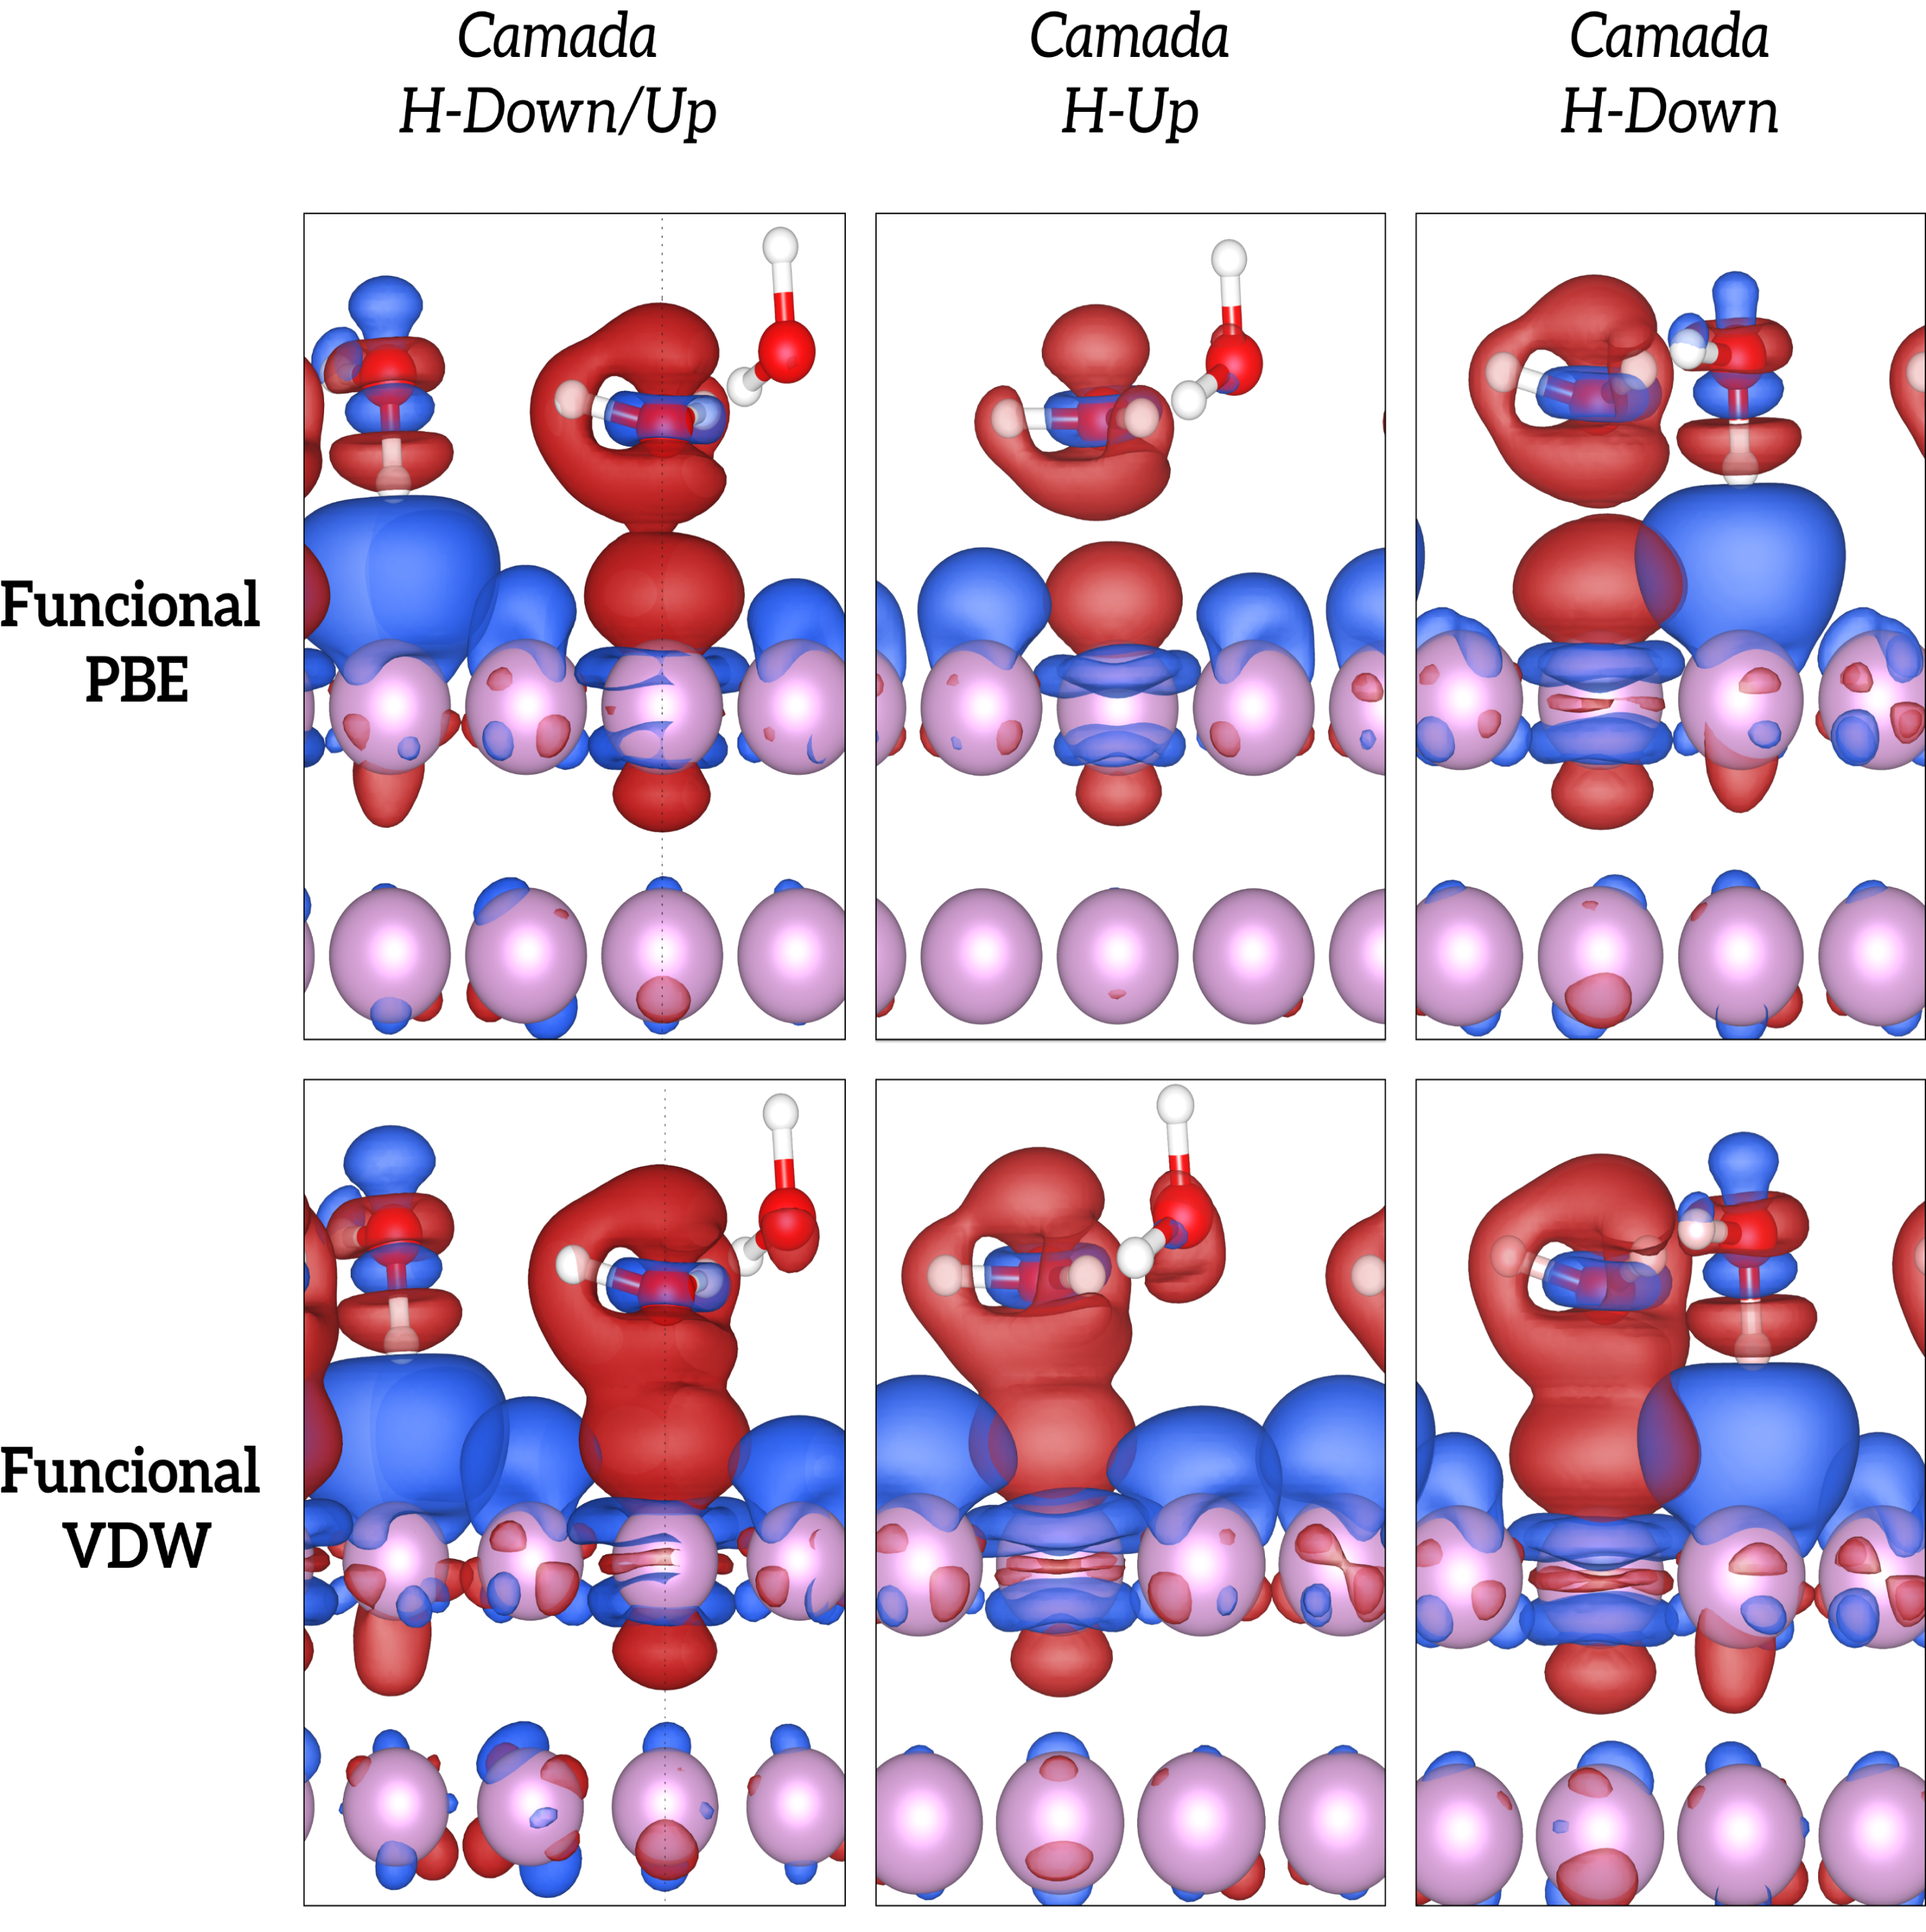
\includegraphics[width=\textwidth]{figs/z_charge.png}
		\legend{Fonte: compilação da autora}
		\label{fig:camada_dens}
	\end{subfigure}
	\begin{subfigure}{0.8\textwidth}
		\caption{\textit{Diferença de Densidade de Carga Média ao longo do eixo z.}}
		\centering
		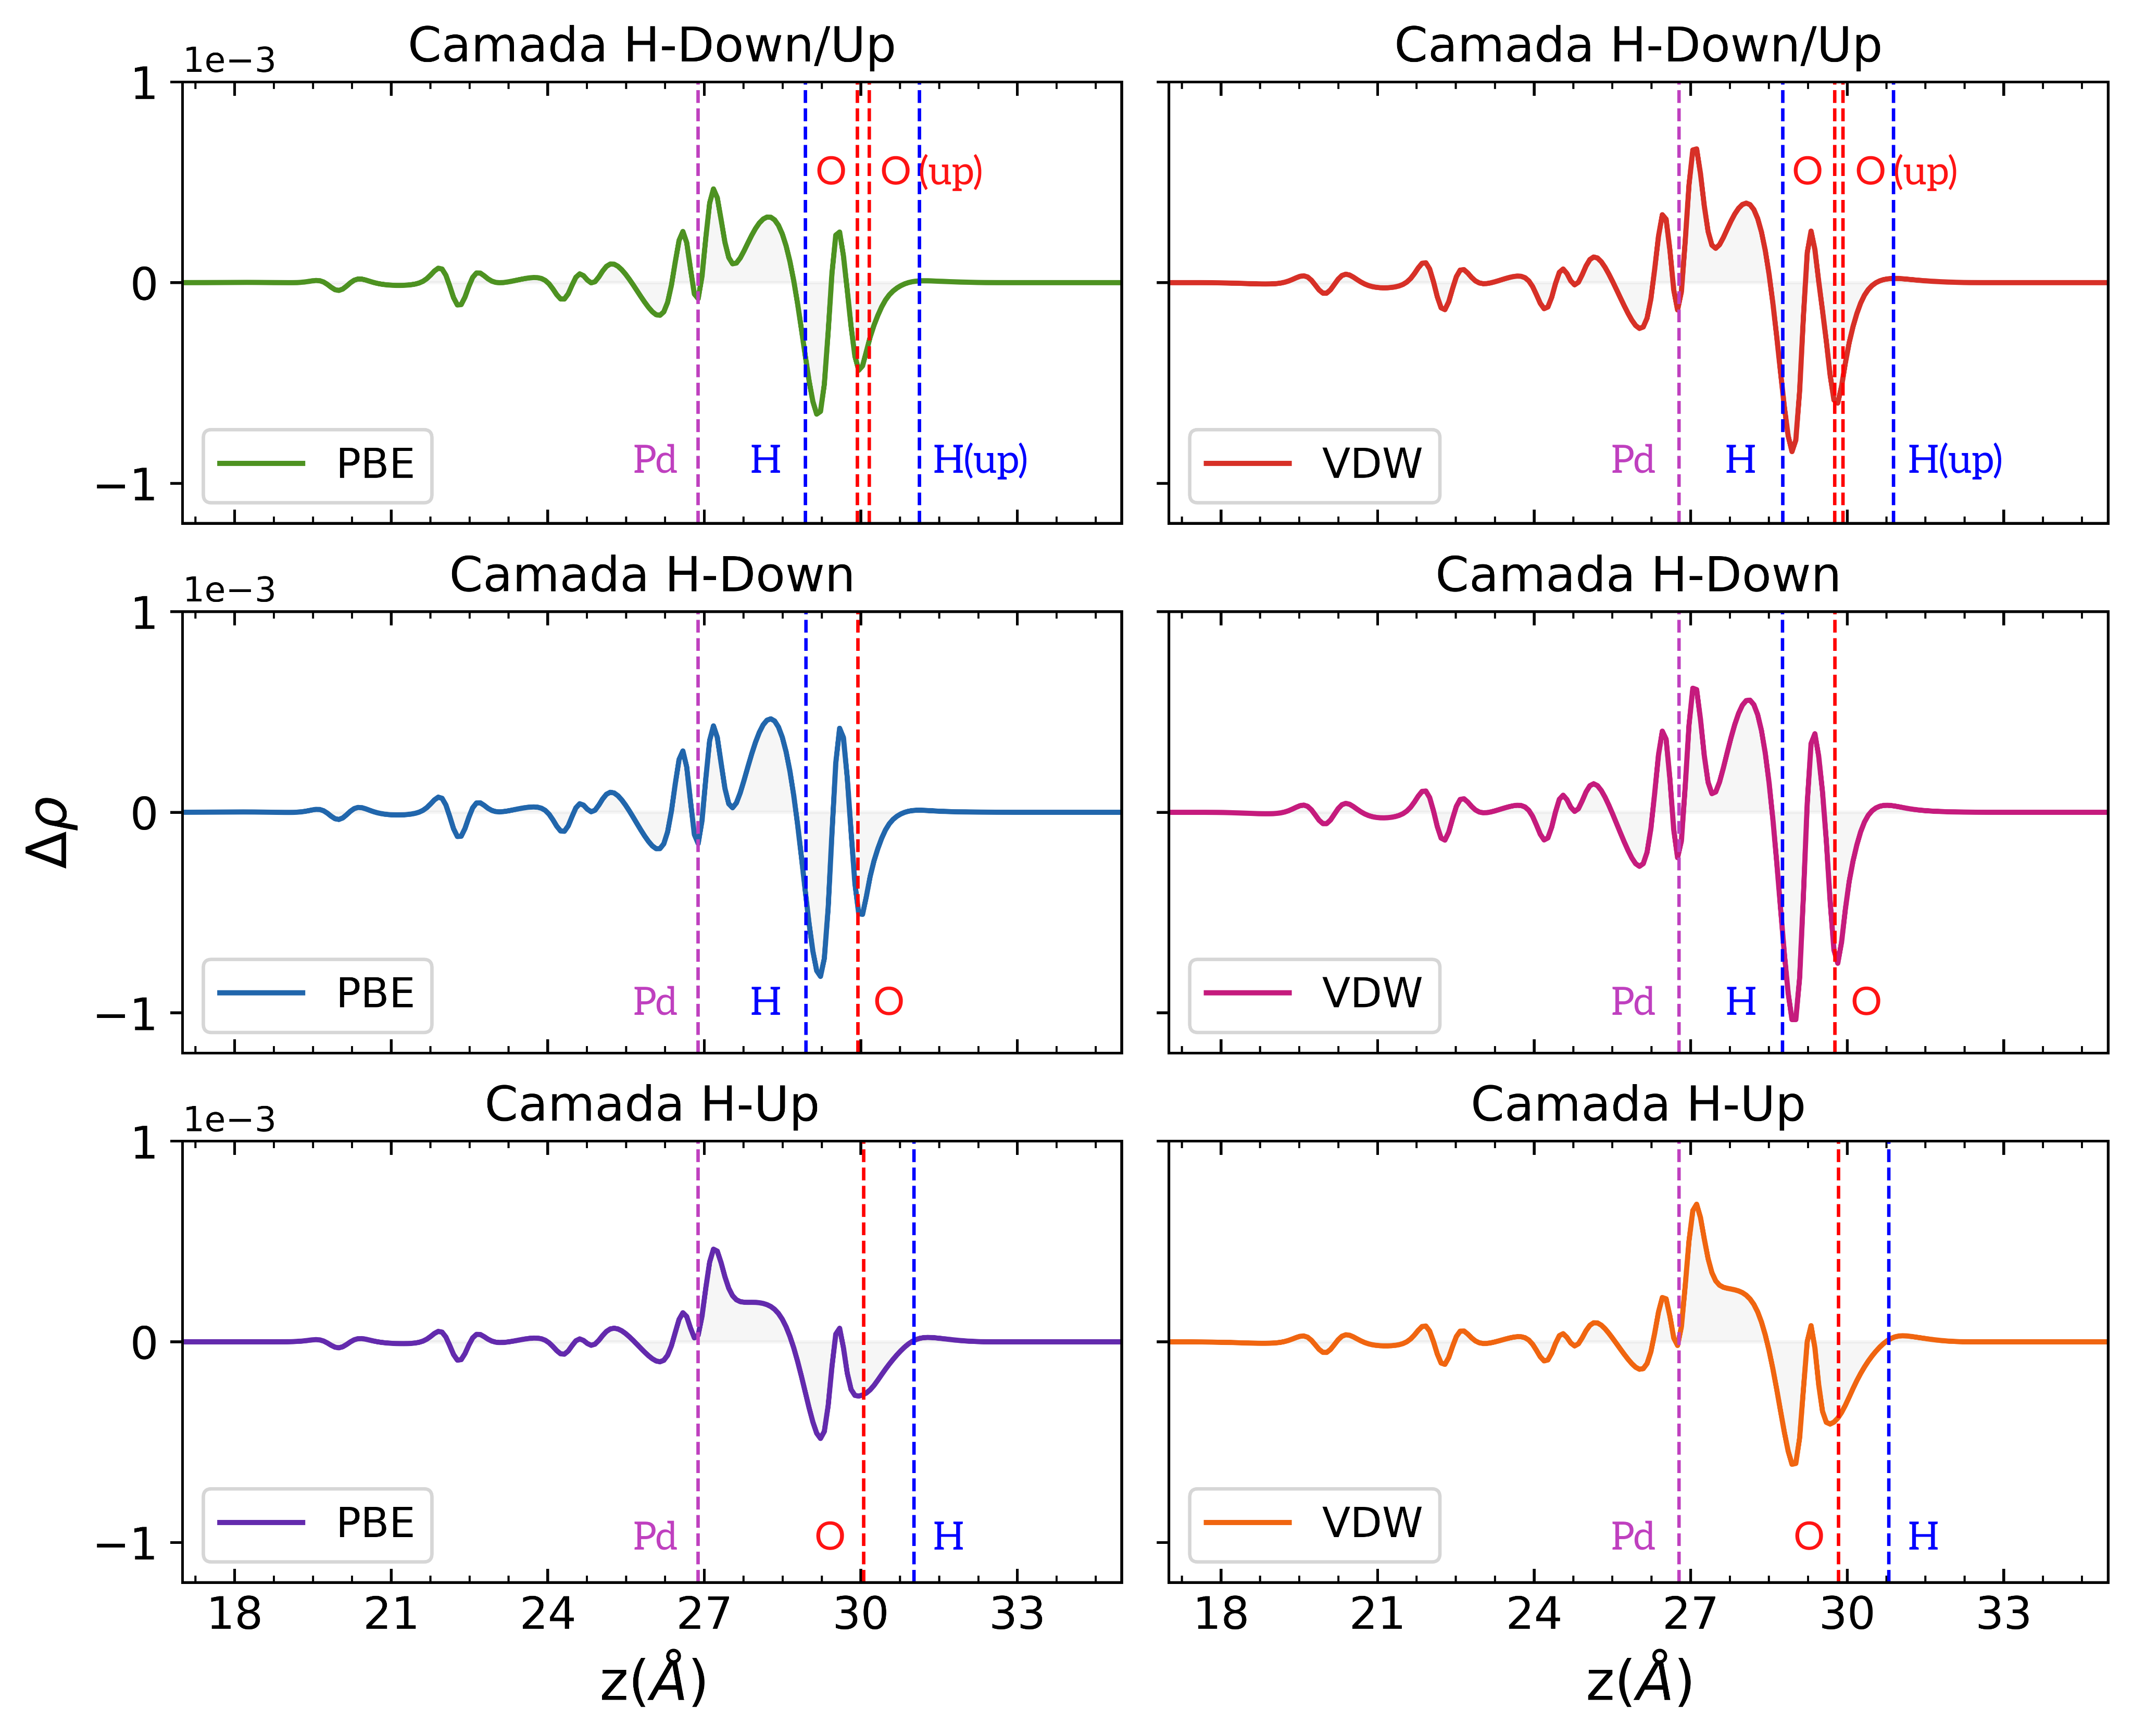
\includegraphics[width=\textwidth]{figs/pd_camada_z.png}
		\legend{Fonte: compilação da autora.}
		\label{fig:camada_z}
	\end{subfigure}
\end{figure}


Através do gráfico de diferença de carga média ao longo do eixo z (Figura \ref{fig:camada_z}), observa-se que as os valores de $ \Delta\rho $ foram maiores com o funcional VDW-BH. Para a camada H-Down, observa-se que o efeito das moléculas \textit{flat-down} sobre $ \Delta\rho $ é mais intenso. Em particular, na região entre a molécula \textit{flat-down} e o metal nota-se uma diminuição acentuada no valor de $ \Delta \rho $. Por outro lado, as modificações que ocorrem na camada \textit{H-Up} são exclusivamente devido à molécula \textit{flat}, visto que as moléculas \textit{flat-up} não interagem diretamente com o metal. A camada H-Down/Up preserva as características das duas outras camadas, porém a interação da molécula \textit{flat-down} é menos intensa. Para compreender melhor como essas interações afetam a estrutura intramolecular das moléculas de água investigaremos na próxima seção os modos normais de vibrações. 


\subsection*{Modos normais de vibração}

Com o intuito de corroborar e completar as análises estruturais e energéticas realizadas e analisar o efeito da adsorção no metal sobre as ligações de hidrogênio, calculamos para cada estrutura as frequências de vibrações dos modos normais. Isso possibilitou identificar as frequências relacionadas à cada tipo de interação (água-água e água-metal). Para representar as frequências do sistema, utilizamos uma distribuição normalizada, uma vez que nosso sistema é composto por 16 moléculas e a quantidade de modos normais de vibrações são dados por $ 3\times N-6 $. Assim, na Figura \ref{fig:modos} está a distribuição para cada funcional, bem como as frequências do dímero isolado experimental (linha pontilhada). Na Tabela \ref{tab:modos}, representamos os valores inferiores e superiores das frequências de \textit{stretching} e o valor central da frequência de \textit{bending}.

Através dessas frequências podemos obter informações sobre a intensidade da ligação de hidrogênio e sobre as interações água/metal, uma vez que é possível relacionar as frequências com as respectivas interações. Essas análises são feitas comparando os valores da camada adsorvida com os valores do dímero no vácuo e explorando as modificações provocadas pelo metal. Por exemplo, uma alta frequência do modo de \textit{stretching} indica uma fraca ligação O-H e também uma ligação de hidrogênio menos intensa e vice-versa. Assim, através dos modos normais de vibrações podemos analisar qual interação é mais dominante em cada estrutura \cite{ref-modos}.
%Modos Normais - Camada
\begin{table}[b!]
	\centering
	\caption{Tabela contendo as principais frequências de vibração da camada adsorvida de acordo com cada funcional, bem como as frequências experimentais e teóricas do dímero isolado. \label{tab:freq-camada}}
	\begin{threeparttable}
		\begin{tabular}{cccccccccc} 
			\hline\hline\addlinespace[3.6pt]
			\multicolumn{10}{c}{\textbf{Frequências dos Modos Normais (cm$ ^{-1} $) - Camada de Água}}                                                                                                                                         \\ 
			\midrule
			\multirow{3}{*}{}                                                &  & \multicolumn{2}{c}{\multirow{2}{*}{Bending}} &  & \multicolumn{5}{c}{\textit{Stretching} (S)}                                                                                                                          \\
			&  & \multicolumn{2}{c}{}                         &  & \multicolumn{2}{c}{Inferior}                                               &  & \multicolumn{2}{c}{Superior}                                                \\ 
			\cmidrule{3-4}\cmidrule{6-10}
			&  & PBE  & VDW                                &  & PBE  & VDW                                                                 &  & PBE  & VDW                                                                 \\ 
			\midrule
			H-Down                                                         &  & 1695 & 1683                                  &  & 3193 & 3051                                                                &  & 3500 & 3428                                                                 \\ 
			
			H-Up                                                           &  & 1664 & 1642                                  &  & 3292 & 3228                                                                &  & 3823 & 3777                                                                 \\ 
			
			H-Down/ Up                                                 &  & 1682 & 1664                                  &  & 3101 & 3180                                                                &  & 3803 & 3774                                                                 \\\midrule  Dímero Isolado            &  & 1668 & 1661                                 &  & \begin{tabular}[c]{@{}c@{}}3612\\3857\end{tabular} & \begin{tabular}[c]{@{}c@{}}3605\\3841\end{tabular}                                                                &  & \begin{tabular}[c]{@{}c@{}}3776\\3875\end{tabular} & \begin{tabular}[c]{@{}c@{}}3752\\3850\end{tabular}                                                                 \\ 
			\midrule Dímero Isolado Exp.\tnote{$\dagger$} &  & \multicolumn{2}{c}{1618.1}                   &  & \multicolumn{2}{c}{\begin{tabular}[c]{@{}c@{}}3547.5\\ 3697.7\end{tabular}} &  & \multicolumn{2}{c}{\begin{tabular}[c]{@{}c@{}}3625.5\\3714.7\end{tabular}}  \\
			\hline\hline
		\end{tabular}
		\begin{tablenotes}\footnotesize
			\item[$\dagger$]\citeauthor{ref-modos}
		\end{tablenotes}
	\end{threeparttable}
	\legend{Fonte: compilação da autora.}
\end{table}




Em relação às frequências de \textit{stretching} do dímero isolado experimental, temos que as frequências $3547.5$ e $3697.7\,\si{cm}^{-1}$ correspondem às frequências de \textit{stretching} simétrico (S) e assimétrico (AS) da molécula doadora, respectivamente, de modo que o menor valor correspondente à ligação O-H que participa da ligação de hidrogênio; as frequências $3625.5$ e $3714.7\,\si{cm}^{-1}$ correspondem às frequências de \textit{stretching} S e AS molécula receptora. Comparando as frequências do dímero isolado obtidas com os funcionais PBE e VDW-BH em relação ao valor experimental, vemos que os valores estão superestimados em média $ 3.3\% $. 
\begin{figure}[t!]
	\centering
	\caption{Distribuição das frequências ($\si{cm}^{-1}$) de vibrações das camadas de acordo com o funcional utilizado. As linhas sólidas e tracejadas correspondem aos funcionais PBE e VDW-BH, respectivamente; as linhas pontilhadas são as frequências experimentais do dímero isolado.}
	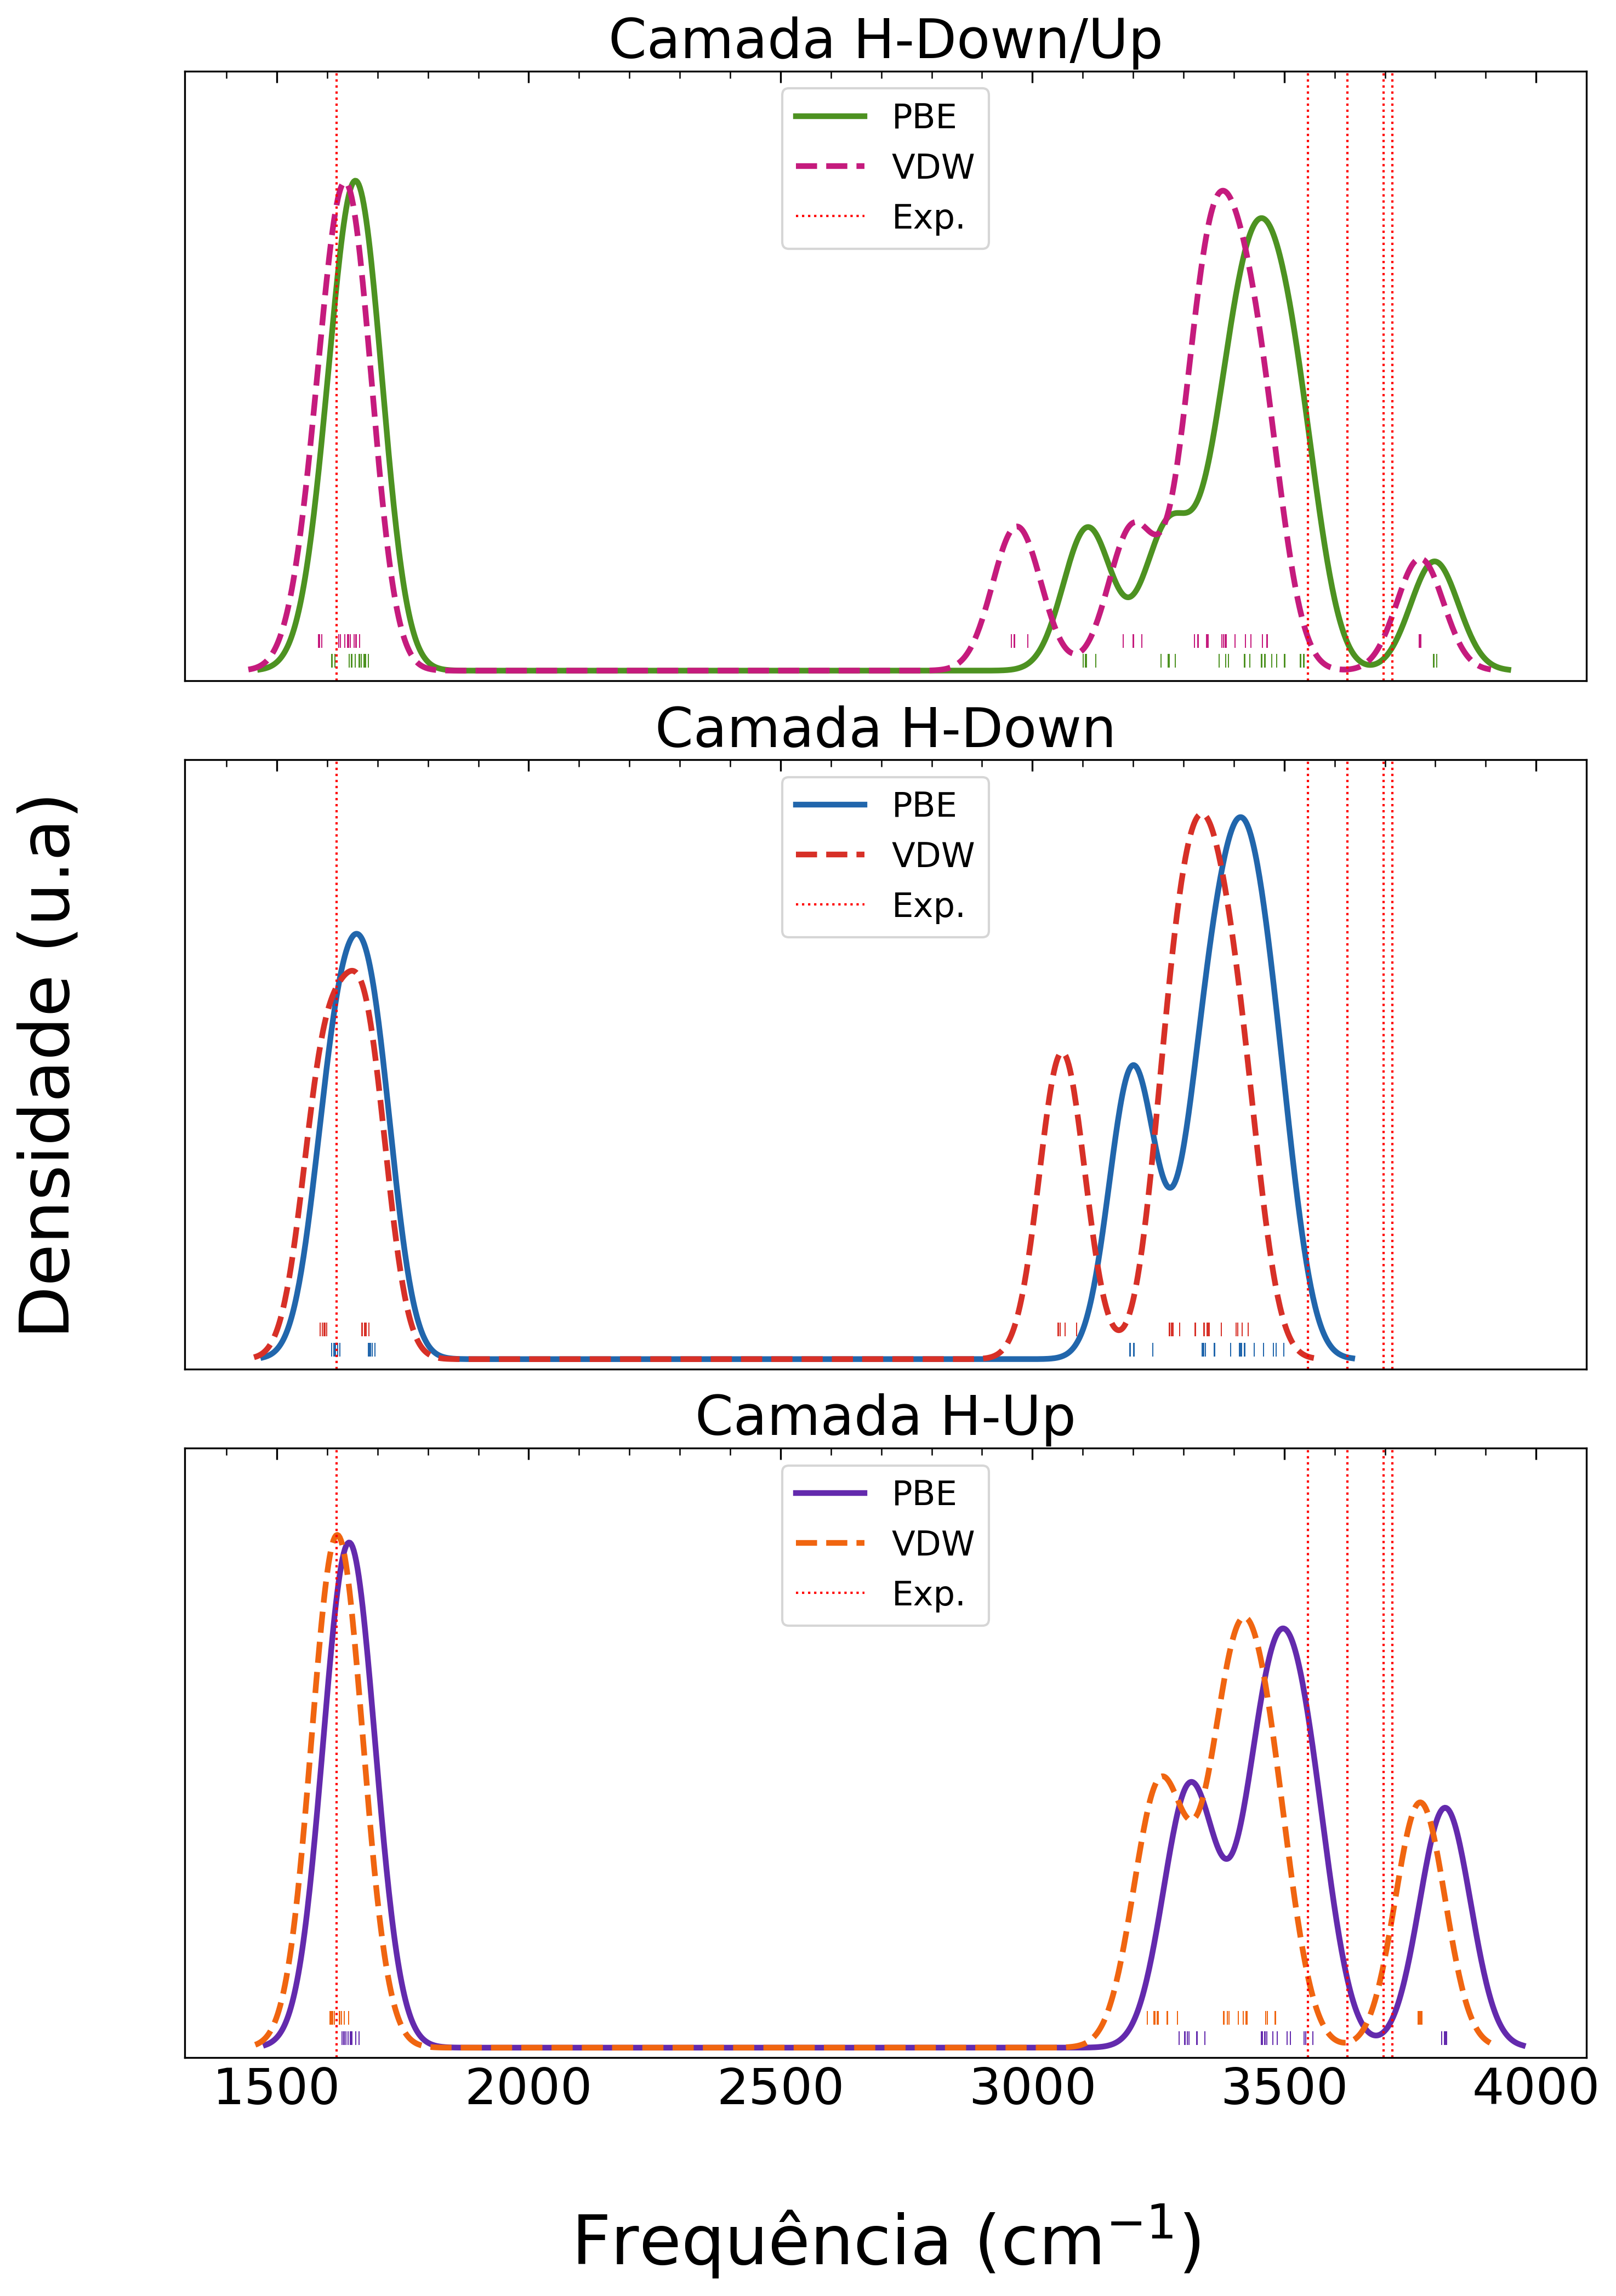
\includegraphics[scale=0.4]{figs/graph_pbe.png}
	\legend{Fonte: compilação da autora.} 
	\label{fig:modos}
\end{figure}

Analisando as frequências da Tabela \ref{tab:modos}, vemos que \textit{bending} da camada H-Up é menor que o valor calculado para o dímero isolado, em especial para o funcional VDW-BH. Isso acontece porque nas moléculas \textit{flat-up} uma ligação O-H participa da ligação de hidrogênio e a outra não se liga ao metal, diferentemente das camadas H-Down e H-Down/Up. Portanto, a camada H-Up é a que possui a intensidade da ligação de hidrogênio mais fraca. Essa observação é também sustentada pelas frequências de \textit{stretching}, onde os maiores valores pertencem à camada H-Up. Por outro lado, as frequências de \textit{stretching} da camada H-Down constituem os menores valores. Esse resultado mostra o efeito da interação com o metal nos modos normais de vibração. A camada H-Down/Up apresenta as propriedades semelhantes às outras duas, com a frequência de \textit{stretching} inferior próxima a da H-Down e a frequência \textit{stretching} superior próxima a H-Up. 

Quando tratamos da frequência de vibração do dímero, temos bem definido quais frequências pertencem às ligações O-H das moléculas doadoras e das receptoras. Entretanto, quando estudamos as camadas adsorvidas, temos além da ligação de hidrogênio a interação com o metal. Ou seja, temos as vibrações da ligação O-H das moléculas \textit{flat} que fazem ligação de hidrogênio e atuam como doadoras ou receptoras; as ligações O-H das  moléculas \textit{flat-up} e \textit{flat-down} que participam das ligações de hidrogênio como doadoras; além das ligaçoes O-H que interagem com o metal (\textit{flat-down}) ou que estão ``livres'' (\textit{flat-up}). 

Analisando a camada H-Down para ambos funcionais, temos 4 picos de frequências de \textit{stretching}, onde um está mais afastado dos demais. Através de uma animação realizada no Programa \textit{Jmol}\footnote{As animações estão disponíveis no link: \url{https://shre.ink/u5l}} é possível ver que, o primeiro pico corresponde à interação da molécula \textit{flat-down} com o metal; o seguinte corresponde à ligação O-H da molécula \textit{flat-down} que faz ligação de hidrogênio e os demais correspondem às moléculas \textit{flat}. Além disso, nota-se que todos os picos dessa camada estão abaixo das frequências do dímero experimental. Como frequências de \textit{stretching} mais baixas correspondem a intensidade das ligações de hidrogênio maiores, então a adsorção no metal fortalece a ligação de hidrogênio. 

Em relação a camada H-Up, o pico de maior frequência está relacionado à ligação O-H que não faz ligação com o metal e as demais estão relacionadas às ligações O-H que participam das ligações de hidrogênio. Por fim, como foi dito anteriormente, a camada H-Down/Up preserva as propriedades de ambas camadas, de modo que os primeiros picos correspondem às interações das moléculas \textit{flat-down} com o metal, o último refere-se às ligações O-H da molécula \textit{flat-up} que estão ``livres'' e os demais correspondem às interações água/água.


Por fim, após caracterizar a adsorção de camadas de água sobre o metal, vimos que o metal intensifica a ligação de hidrogênio entre as moléculas de água através da diminuição da distância $ d_{OO} $. Além disso, vimos que a camada H-Down é mais estável energeticamente e provoca uma diminuição de densidade de carga na região entre a molécula \textit{flat-down} e o metal. Por outro lado, a presença de moléculas \textit{flat-down} na camada H-Down/Up também a torna estável, uma vez que essa camada preserva as características da camada H-Down. Através das propriedades vibracionais, vimos que a interação com o metal apresenta frequências de \textit{stretching} menores que as frequências correspondentes às ligações de hidrogênio. Nesse capítulo caracterizamos a interface água/metal sem a presença de uma pertubação externa ao sistema. No próximo capítulo analisaremos se as caracterizações aqui realizadas são afetadas pela presença de um potencial externo.

\chapter{Potencial Externo Aplicado à Interface Água/Metal \label{cap:bias}}
%% Introdução Geral falando sobre os cálculos fora do equilíbrio

Descrever a interface água/metal é fundamental para compreender processos de rearranjo e transferência de carga que ocorrem na dupla camada elétrica (\textit{Electric Double Layer} -- EDL). No entanto, realizar simulações computacionais que descrevam uma célula eletroquímica de forma mais realística é um desafio devido à dificuldade de incluir tanto o eletrólito, quanto a aplicação de potencial externo sobre os eletrodos. Além disso, a aplicação de um potencial externo sobre a interface água/metal afeta a reatividade do metal e as interações com a água. Não obstante, a água apresenta comportamentos complexos e distintos que são sensíveis ao substrato e às condições estruturais. Nesse sentido, simulações computacionais que consideram perturbações externas ao sistema são fundamentais para compreender as alterações que ocorrem na interface água/metal em situações mais realísticas. 

Nesse capítulo estudamos um modelo protótipo de uma célula eletroquímica, no qual um potencial externo é aplicado à interface água/metal. Esse modelo permitiu estudar as modificações estruturais das moléculas de água adsorvidas em eletrodos metálicos de Paládio e Ouro. Esses dois metais possuem características distintas e se destacam pela resposta eletroquímica. O Pd é um metal mais reativo que outros metais platinados e possui afinidade em relação às ligações envolvendo hidrogênio e oxigênio \cite{paladio}. Embora o Au seja um metal nobre e inerte, cuja superfície é resistente à oxidação e menos reativo, ele apresenta uma alta atividade eletrocatalítica \cite{ouro}.

Dessa forma, aplicamos um potencial externo sobre o sistema através do formalismo de Funções de Green Fora do Equilíbrio e analisamos o efeito do potencial sobre as propriedades estruturais e vibracionais. Através desse formalismo o sistema é inteiramente tratado atomisticamente por meio de cálculos de primeiros princípios. Para o Pd(111), estudamos o efeito do potencial externo sobre um monômero adsorvido na superfície metálica (Seç. \ref{sec:pd_negf}), ao passo que para o Au(111) foi investigado a adsorção do monômero e de uma camada de água (Seç. \ref{sec:au_negf}). 

	
\section{Paládio\label{sec:pd_negf}}

Após caracterizar as propriedades eletrônicas e vibracionais da interface água/Pd(111) sem a presença de perturbações externas ao sistema (vide Cap. \ref{cap:equilibrio}), obtivemos tais propriedades considerando um potencial externo aplicado a fim de investigar o efeito do potencial sobre a interação água/metal. Para isso, utilizamos o monômero na orientação \textit{flat} adsorvido numa superfície metálica de tamanho $ 3\times4 $. Os eletrodos foram montados com 6 camadas e a denominada região de espalhamento com 4 e 3 camadas de cada lado (Figura \ref{fig:sistema_pd}). As superfícies metálicas eram separadas por um vácuo de $ 25\,\si{\angstrom} $. Os cálculos fora do equilíbrio foram realizados com os funcionais de troca e correlação PBE e VDW-BH. As dimensões das células unitárias utilizadas foram de $ 9.73\times8.42\times66.64\,\si{\angstrom} $ para o funcional PBE e $ 9.58\times8.30\times 67.38\,\si{\angstrom} $ para o VDW-BH, cujos parâmetros de rede foram $ 3.97\,\si{\angstrom} $ e $ 3.91\,\si{\angstrom} $, respectivamente.
\begin{figure}[H]
	\centering
	\caption{Ilustração do sistema utilizado para aplicar um potencial externo sobre a interface água/Pd (111). Além disso, estão ilustrados as regiões que correspondem aos eletrodos e a região de espalhamento.}
\label{fig:sistema_pd}
	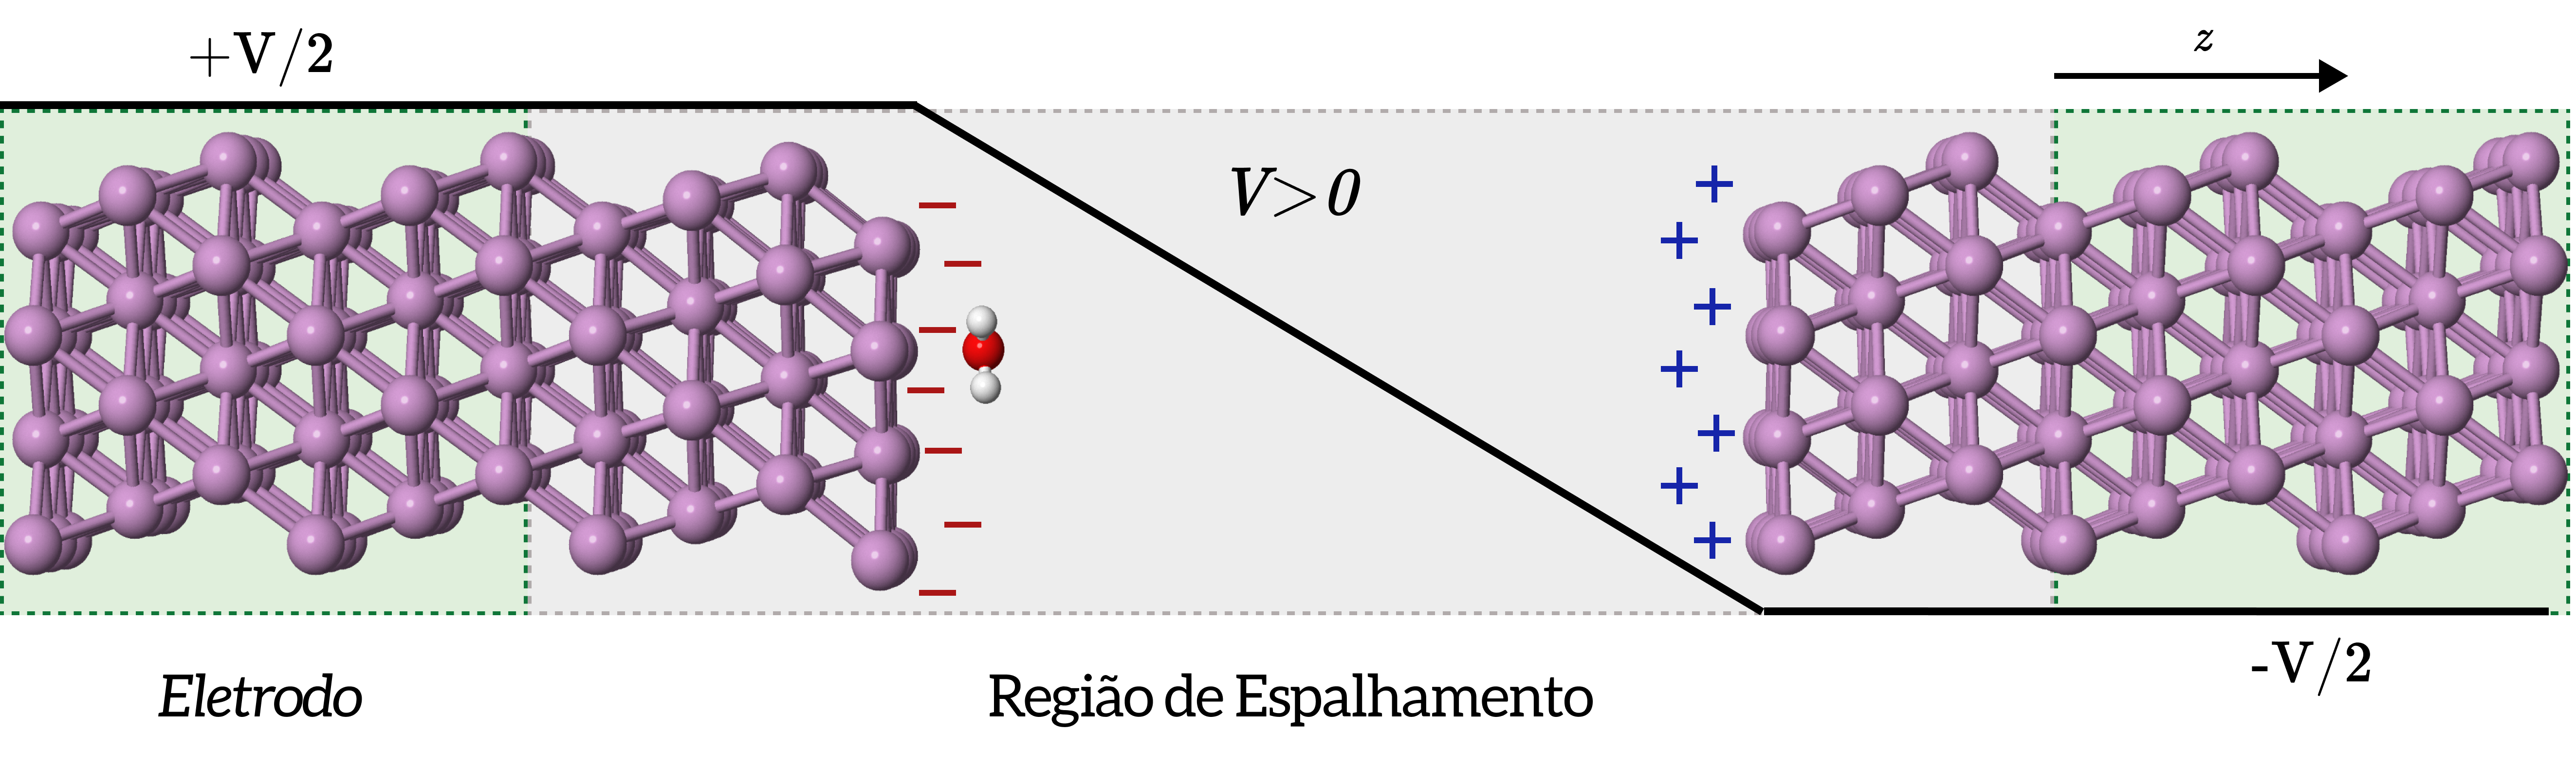
\includegraphics[scale=0.35]{figs/sistema_pd.png}
	\legend{Fonte: compilação da autora.}
\end{figure}

Para aplicar a diferença de potencial externa, primeiramente, determinou-se a geometria de mínima energia utilizando condições periódicas de contorno e em seguida o sistema foi minimizado com o $ V=0.0\,\si{\eV} $ (\textit{potencial 0}). Após a minimização com PBC obteve-se para o funcional PBE $d_{O-Pd}=2.47\,\si{\angstrom} $ e $ \alpha=-4\si{\degree} $ e para o funcional VDW-BH $d_{O-Pd}=2.39\,\si{\angstrom} $ e $ \alpha=2\si{\degree} $. Esses valores coincidem com os obtidos a partir da minimização com \textit{potencial 0}: $d_{O-Pd}=2.46\,\si{\angstrom} $ e $ \alpha=-4\si{\degree} $ para o PBE e $d_{O-Pd}=2.39\,\si{\angstrom} $ e $ \alpha=2\si{\degree} $ para o VDW-BH. Em seguida, com a geometria obtida a partir da otimização com o \textit{potencial 0}, aplicou-se a diferença de potencial entre -2.5 a 2.5 eV com intervalos de 0.5 eV. Com isso, foi possível analisar possíveis transferências de carga através das diferenças de densidade de carga $ \Delta\rho_{V} $ entre o potencial aplicado $ \rho_{V\neq0} $ e $ \rho_{V=0} $. %A análise de diferença de carga foi feita para ambos funcionais (Figura \ref{fig:pd_zcharge}). 

Através do gráfico de $ \Delta\rho_{V} $, percebe-se que a aplicação do potencial externo induz uma pequena transferência de carga entre o metal e a molécula de água (Figura \ref{fig:pd_densidade} e \ref{fig:pd_zcharge}). Além disso, a maior parte dessa diferença está concentrada no átomo de oxigênio e é proporcional ao potencial aplicado. Embora os gráficos de $ \Delta\rho_{ _{+V}} $ e $ \Delta\rho_{ _{-V}} $ sejam semelhantes, observa-se que a flutuação entre essas densidades de carga são assimétricas, ou seja, o efeito do potencial positivo sobre a molécula de água é diferente do negativo (última coluna da Figura \ref{fig:pd_densidade}). Em particular, tem-se que para os potenciais menores ocorre uma flutuação positiva, indicando que nesses casos a interação da molécula com o metal é maior para o potencial positivo. Além disso, observa-se uma polarização de carga superficial na região acima do eletrodo metálico. 

\begin{figure}[t!]
	\centering
	\caption{Variação da densidade de carga dos potenciais aplicados em comparação ao potencial de potencial 0 $ \Delta\rho_{_ {V}}=\rho_{V}-\rho_{0} $ com o funcional PBE. Em todos os recortes foram utilizados o valor de isosuperfície $ 1.80\times10^{-4}\;\si{e}/\si{\angstrom}^3  $ para $ \Delta\rho_{_ {V}} $. Na última coluna está representado a flutuação de densidade de carga entre os potenciais positivos e negativos $ \Sigma\Delta\rho_{_ {V}}=\Delta\rho_{ _{+V}}+\Delta\rho_{ _{-V}} $, onde o valor de isosuperfície é $ 1.67\times10^{-5} \;\si{e}/\si{\angstrom}^3 $. Em todos os casos, azul/vermelho indica uma deficiência/excesso de elétrons.}
	\label{fig:pd_densidade}
	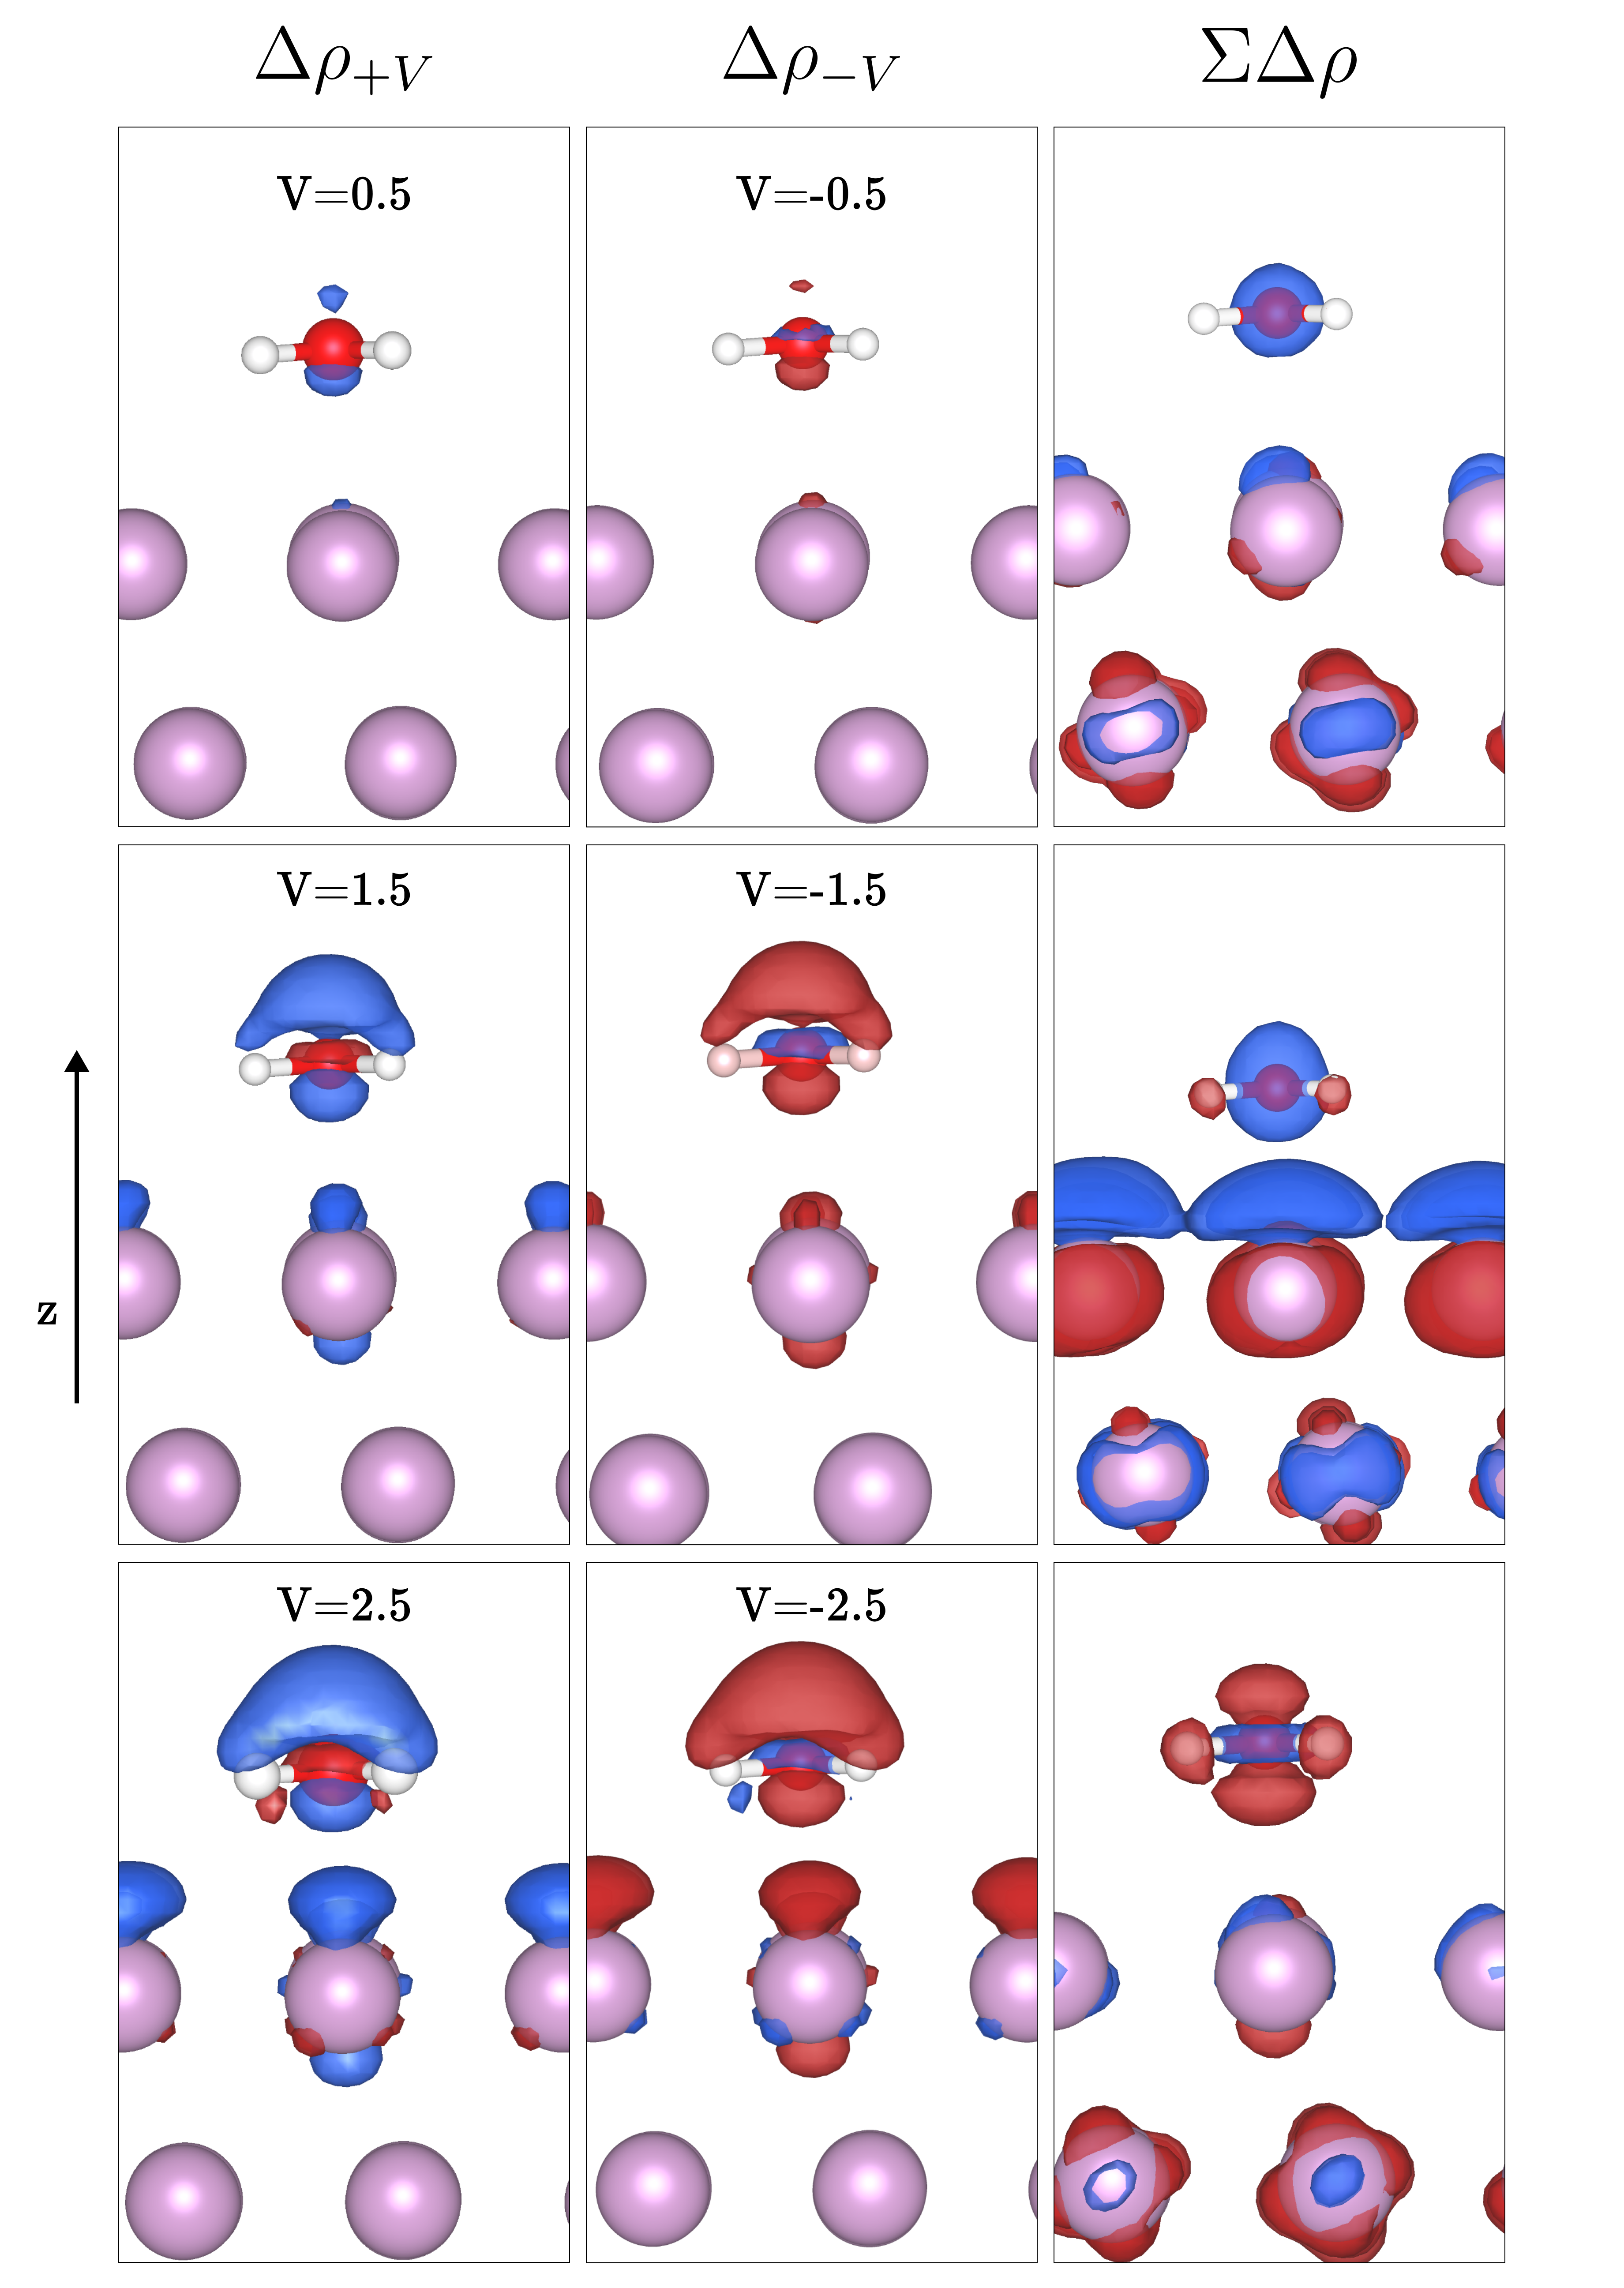
\includegraphics[scale=0.068]{figs/pd_densidade2.png}
	\legend{Fonte: compilação da autora.}
\end{figure}

Considerando as correções com o funcional VDW-BH nos sistemas sem perturbações externas, vimos que as energias de adsorção aumentaram e as propriedades vibracionais foram afetadas. Assim, com o intuito de determinar o efeito das forças de dispersão considerando perturbações externas, comparamos qualitativamente $ \Delta \rho_{V} $ entre os dois funcionais (Figura \ref{fig:pd_zcharge}). Em relação ao funcional VDW-BH, observou-se um comportamento similar ao do PBE através do gráfico de $ \Delta \rho_{V} $ médio ao longo do eixo z para os potenciais $ V=\pm1.5\,\si{\eV}$ e $ V=\pm2.5\,\si{\eV} $ . Ademais, as propriedades geométricas obtidas com a minimização a $ V=0\,\si{eV} $ para os funcionais PBE e VDW-BH, tais como distância $ d_{O-Pd} $ e inclinação $ \alpha $, diferem entre si por $ 0.07\,\si{\angstrom} $ e $ 6\si{\degree} $, respectivamente -- Tabela \ref{tab:neq_geometria_pd}. No entanto, essas variações são similares às obtidas sem perturbações externas (Tabela \ref{tab:geom_pbe} e Figura \ref{fig:neq_pd_mon_freq}). Assim, as ligações responsáveis pelas interações água/Pd na presença dos potenciais externos aqui aplicado não foram significativamente modificadas pela presença do funcional VDW-BH. Esse comportamento também foi observado por \citeauthor{artigo-luana} ao estudar as forças resultantes sobre a molécula de água adsorvida em Au(111) com o funcional VDW-DRSLL$ ^{PBE} $. 


\begin{figure}[t!]
	\centering
	\caption{Comparação da diferença de densidade de carga média ao longo do eixo z dos cálculos com os funcionais PBE e VDW-BH. As densidades foram obtidas nas geometrias correspondentes a cada funcional com os potenciais aplicados $V=\pm 1.5\,\si{\eV} $ e $V=\pm2.5\,\si{\eV}$. As linhas sólidas verticais indicam as respectivas posições dos átomos de Pd abaixo da molécula de água e do átomo de O.}
	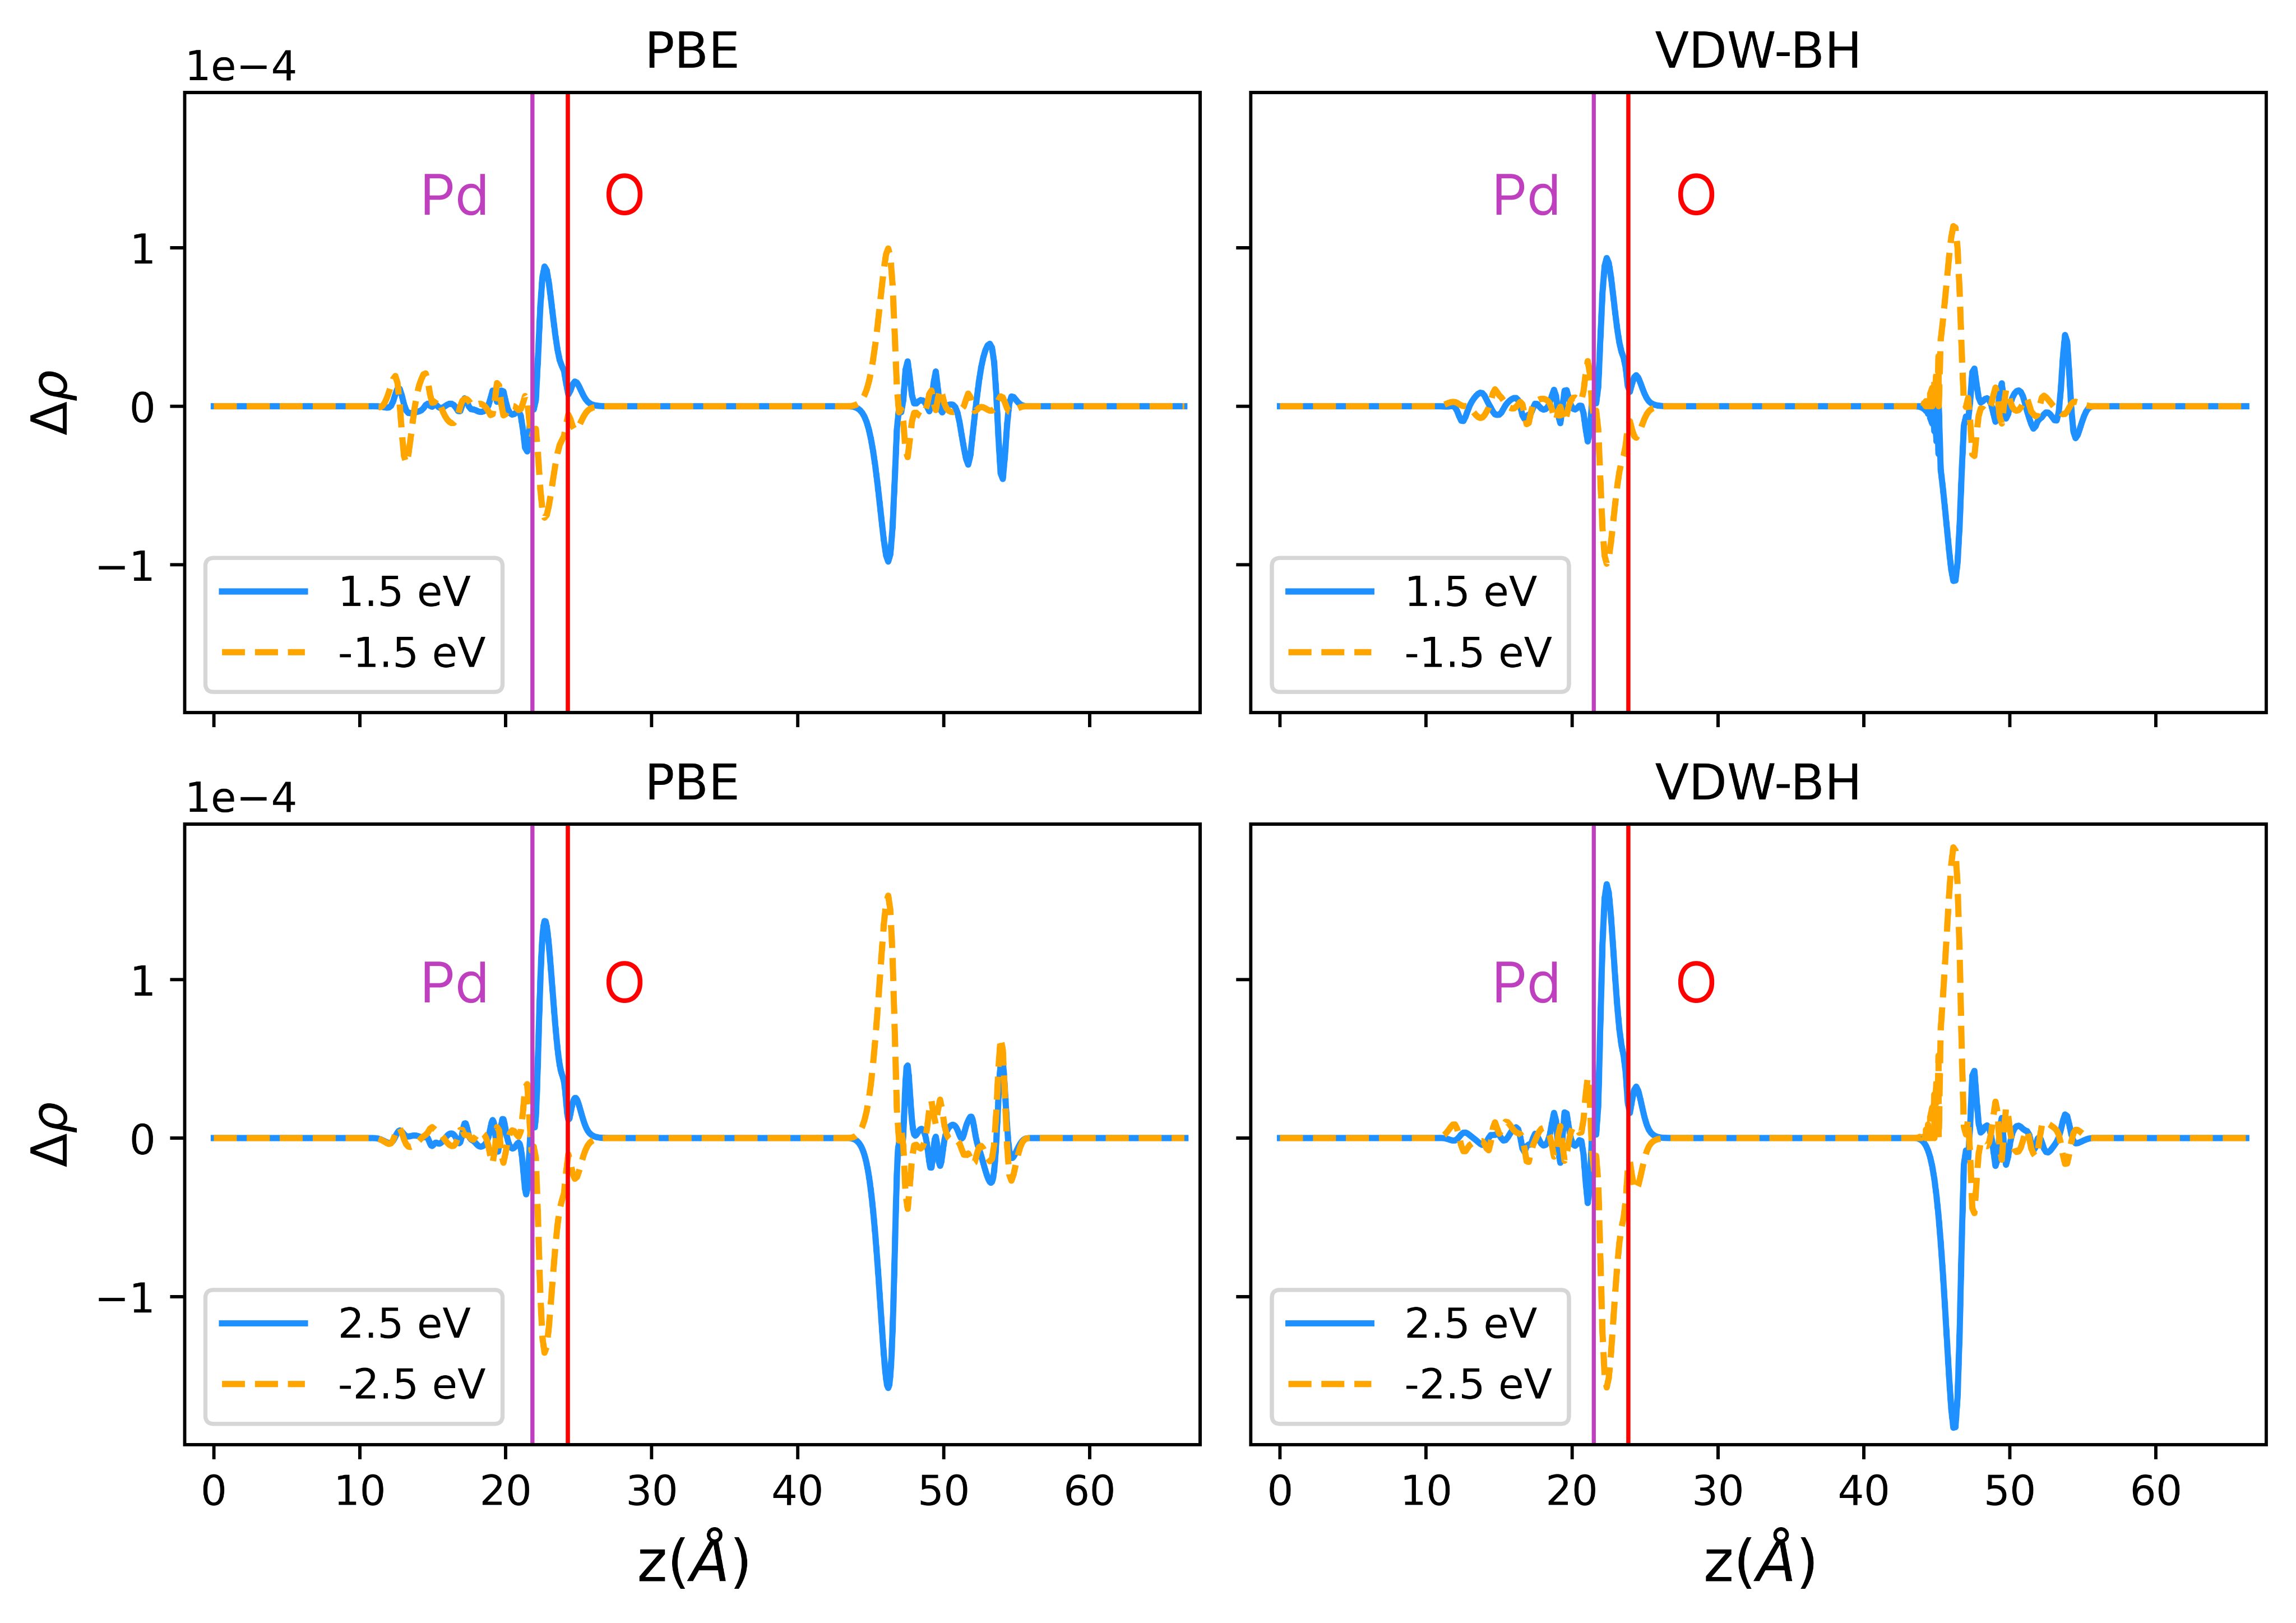
\includegraphics[scale=0.1]{figs/pd_densidade.png}
	\label{fig:pd_zcharge}
	\legend{Fonte: compilação da autora.}
\end{figure}

Tendo em vista que a utilização de correções do tipo vdw não afeta significativamente a descrição do sistema ao aplicar o intervalo de potenciais externos aqui utilizados, então foi realizado a minimização das coordenadas para $ V\neq0 $ utilizando o funcional PBE. Isso permitiu obter as propriedades geométricas (Tabela \ref{tab:neq_geometria_pd} e Figura \ref{fig:neq_pd_mon_geo}) e calcular as frequências dos modos normais de vibrações (Tabela \ref{tab:neq_freq_pd} e Figura \ref{fig:neq_pd_mon_freq}) considerando uma diferença de potencial externa, bem como definir o efeito resultante sobre a ligação água/metal.
\begin{table}[h!]
	\centering
	\caption{Variação das propriedades geométricas da molécula de água adsorvida no Pd(111) em relação ao potencial externo aplicado V obtidas a partir da otimização com o funcional PBE. As propriedades incluem a distância entre o átomo de O e Pd ($d_{O-Pd}(\si{\angstrom})$), o deslocamento lateral ($\Delta Oxy$), a inclinação ($\alpha$), a distância entre os átomos de H e O ($d_{O-H}(\si{\angstrom})$) e o ângulo ($\Theta$) entre os átomos de H. A última linha refere-se à relaxação a 0 bias com o funcional VDW-BH. \label{tab:neq_geometria_pd}}
	\begin{threeparttable}
		\begin{tabular}{Sccccc} 
			\hline\hline\addlinespace[3.6pt]
			\multicolumn{6}{c}{\textbf{Propriedades Geométricas $ H_2O/Pd$}}   \\\midrule
			{V (\si{eV})}   &{$d_{O-Pd}(\si{\angstrom})$} & {$ d_{O-H}(\si{\angstrom})$}  & {$\Delta\, Oxy(\si{\angstrom})$} &{$\Theta(\si{\degree})$}&{$\alpha(\si{\degree})$}\\
			\hline
			2.50		&2.56	&0.98	&0.67	&103&-22 \\
			2.00		&2.53	&0.98	&0.60   &103&-17 \\
			1.50		&2.51	&0.98	&0.55	&103&-13 \\
			1.00		&2.49	&0.98	&0.55	&103&-10\\
			0.50		&2.48	&0.98		&0.49	&102&-6\\
			0.00		&2.46	&0.98	&0.49	&104&-4\\
			-0.50		&2.45	&0.98	&0.43	&104&0 \\
			-1.00		&2.44	&0.98&0.42	&104&3 \\
			-1.50		&2.43		&	0.98/0.97	&	0.38	&104	& 6\\
			-2.00		&2.42	&0.97	&0.26	&104&12 \\
			-2.50		&2.41	&0.97	&0.24	&104&16 \\	
			\midrule
			{0.00}\tnote{$\dagger$} 	&2.39	&0.98	&0.35	&104&2\\%\\{PBC}&2.47&0.98&0.49&104&-4\\		
			\hline\hline
		\end{tabular}
		\begin{tablenotes}\footnotesize
			\item[$\dagger$] Funcional VDW-BH
		\end{tablenotes}
	\end{threeparttable}
	\legend{Fonte: compilação da autora.}
\end{table}

\begin{figure}[h!]
	\centering
	\caption{Variação da inclinação $ \alpha $ e da distância $ \Delta d_{O-Pd} $ de acordo com o potencial externo aplicado. O valor de $ \Delta d_{O-Pd}=d_{O-Pd,V}-d_0 $ mensura o quanto a molécula se afastou em relação à posição inicial $ d_0=2.46\,\si{\angstrom} $. Além disso, também estão ilustrados as posições do monômero em relação à superfície metálica.}
	\label{fig:neq_pd_mon_geo}
	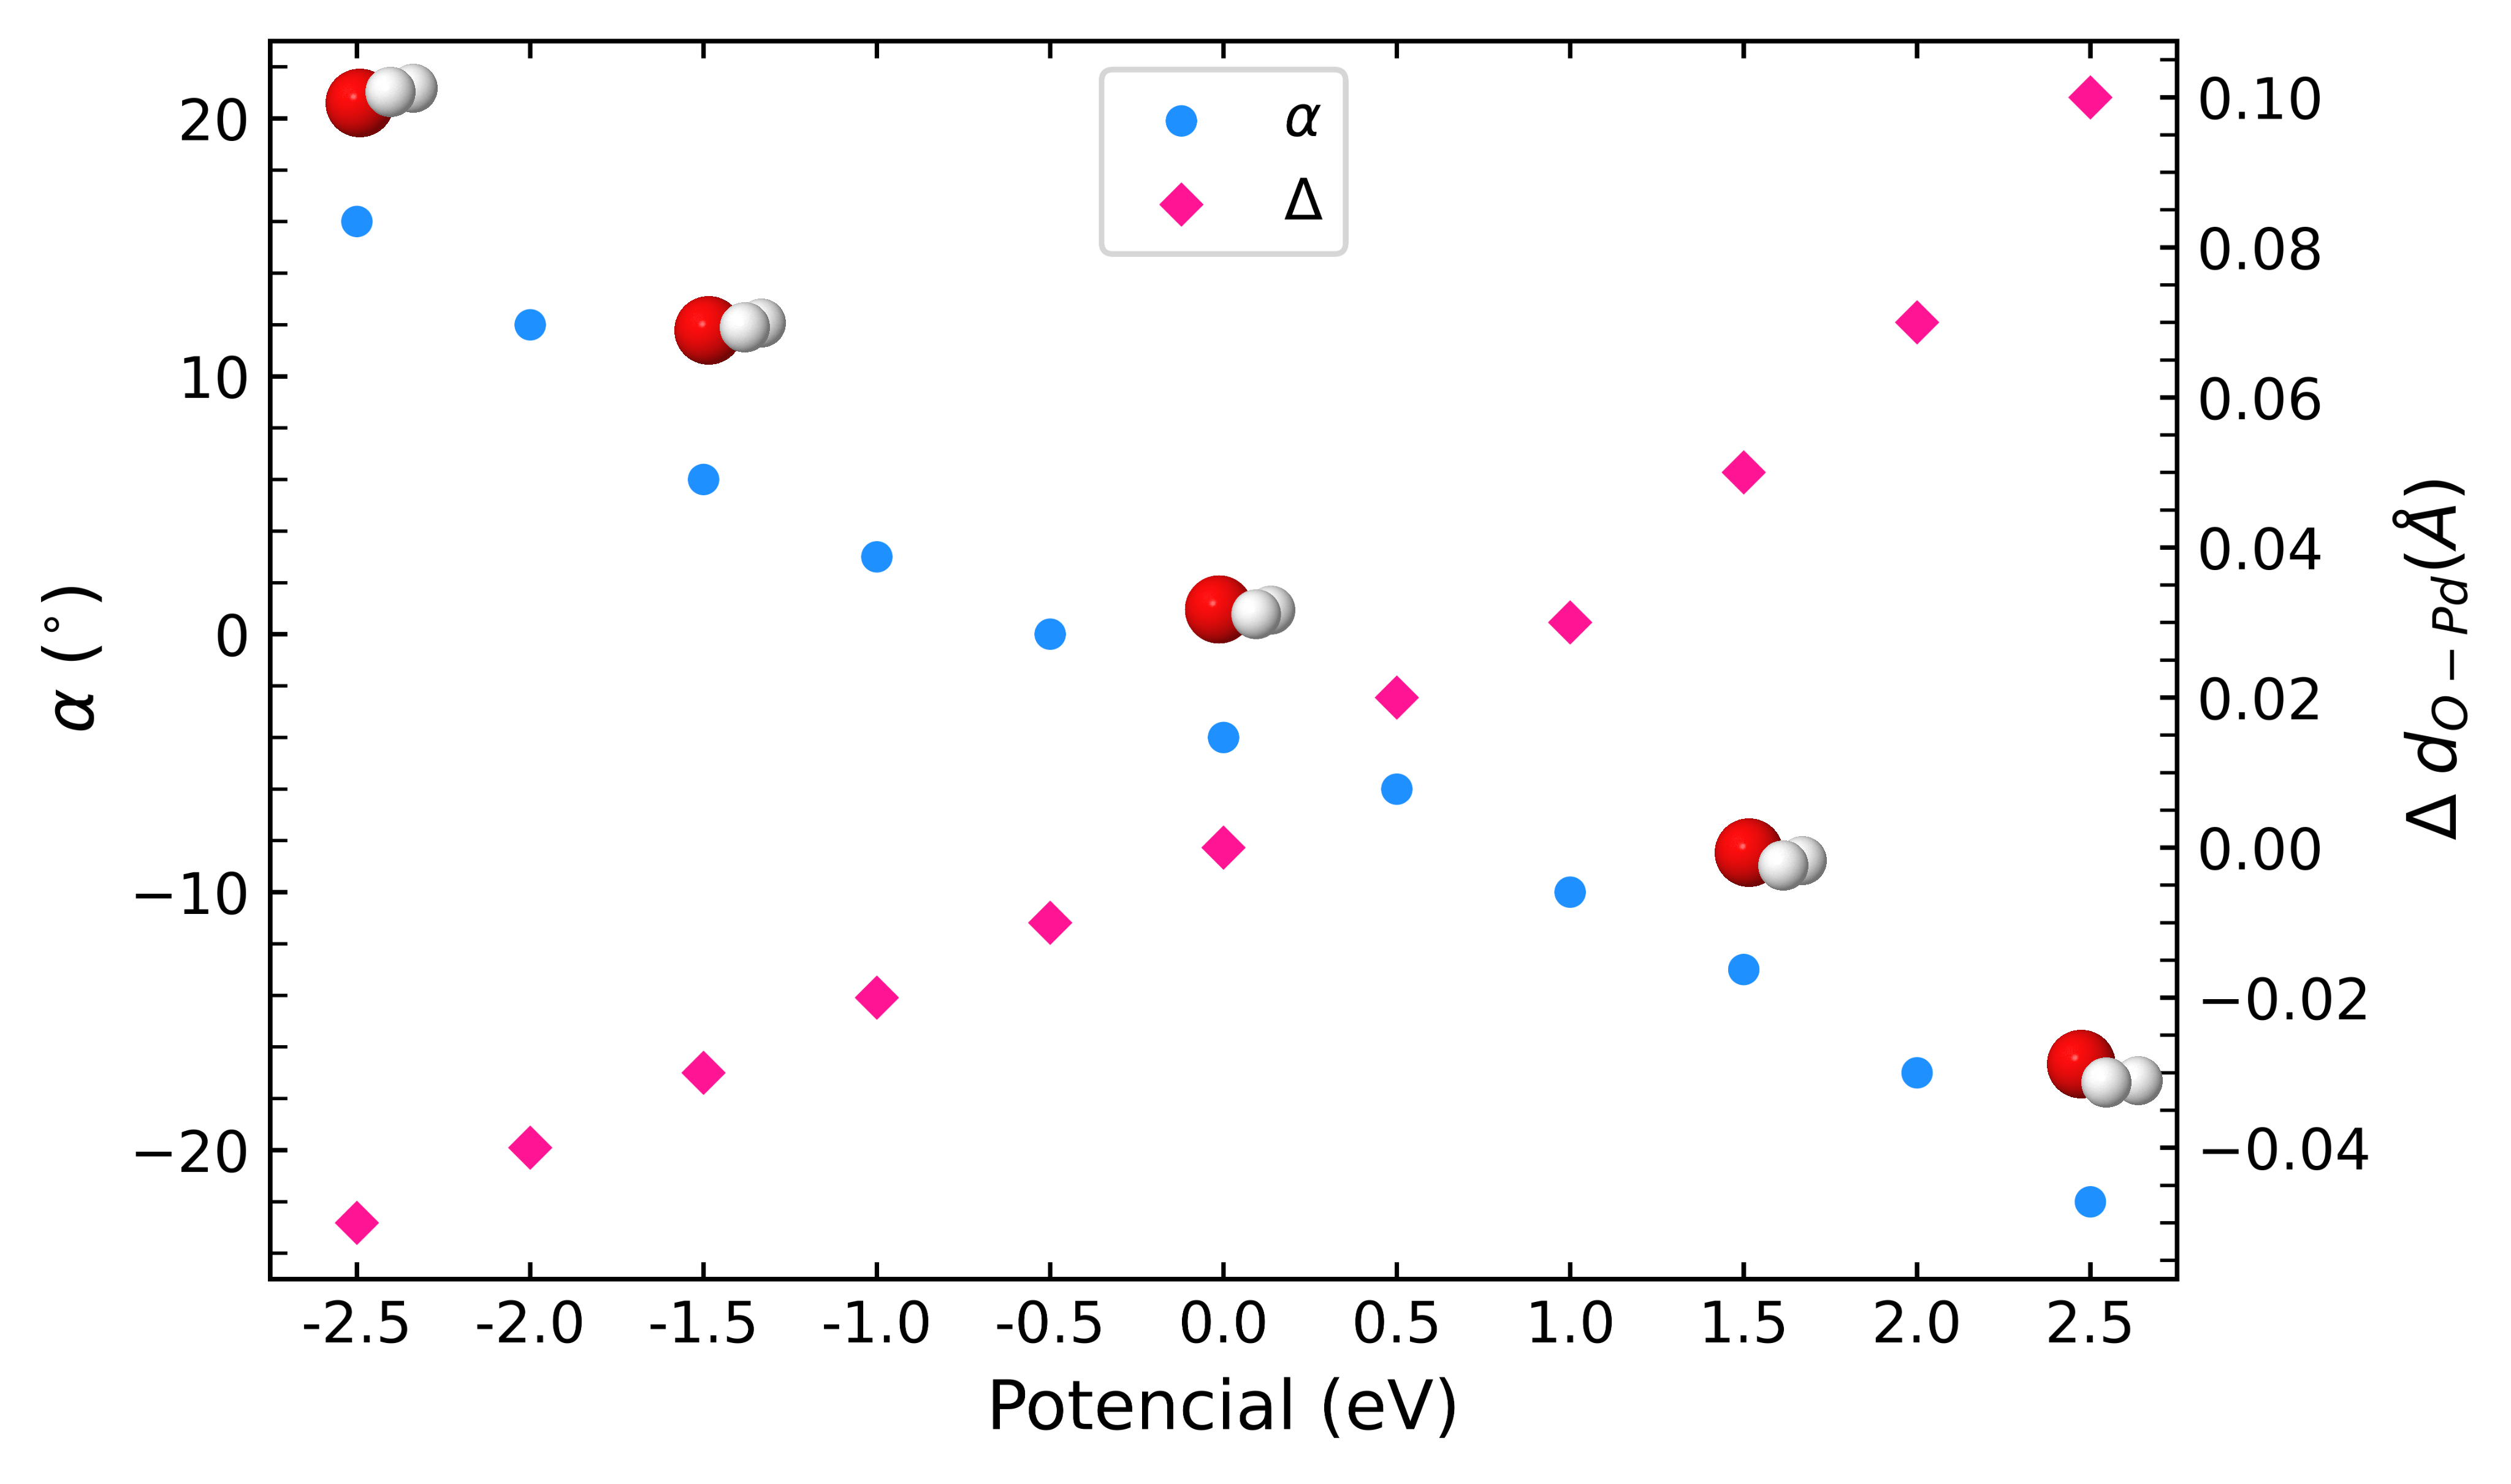
\includegraphics[scale=0.088]{figs/monomero_pd_ang.png}
	\legend{Fonte: compilação da autora.}
\end{figure}

Sem a presença de perturbações externas, a interação água/metal ocorre através da interação do orbital $ b_1 $ com os níveis vazios do Pd. No entanto, ao aplicar uma diferença de potencial ao sistema, a interação resultante vai ser uma combinação do efeito eletrostático e da interação água/metal. Assim, analisando o efeito dessa combinação, nota-se uma tendência da molécula de se aproximar do metal para $ V<0 $ e de se afastar do metal para $ V>0 $ (Figura \ref{fig:neq_pd_mon_geo}). Isso ocorre devido à polarização de carga superficial negativa/positiva no metal que surge ao aplicar um potencial positivo/negativo sobre o eletrodo metálico. O efeito dessa polarização aparece nos gráficos de densidades de carga, no qual, acima da superfície, tem-se uma concentração de densidade de carga representando a deficiência/excesso de elétrons (Figura \ref{fig:pd_densidade}). 

Dessa forma, essa polarização superficial afeta a interação eletrostática entre o metal e a molécula de água, ora atraindo-a, ora repelindo-a. Logo, para $ V>0 $ ocorre um aumento máximo de $ 0.1\,\si{\angstrom} $ da distância $ d_{O-Pd} $ e uma redução máxima de $ -18\si{\degree} $ da inclinação da molécula de água $ \alpha $, ao passo que para $ V<0 $ o átomo de O é atraído para a superfície metálica em até de $ 0.05\,\si{\angstrom} $ e rotaciona em até $ 20\si{\degree} $. É possível notar que as mudanças em $d_{O-Pd}$ e $\alpha$ dependem do sinal de V, em concordância com o comportamento assimétrico observado nos gráficos de $\Delta\rho_{V}$. Assim, esse comportamento assimétrico está relacionado às alterações estruturais que ocorrem nas moléculas de água, visto que a molécula de água altera a sua orientação e consequentemente, a interação entre a água e o metal são alteradas. Portanto, o sinal do potencial aplicado afeta o comportamento da molécula de água e a interação com o metal.

% que afetam o \textit{overlap} entre os orbitais da molécula de água e os da superfície



Além do efeito eletrostático sobre a interação água/metal, observa-se também, como resultado da aplicação do potencial externo alterações na repulsão de Pauli. Para definir a contribuição dessa interação, \citeauthor{artigo-luana} separaram a contribuição do campo elétrico das demais interações e associaram o efeito resultante da interação água/metal ao aumento (diminuição) da repulsão de Pauli. Dessa forma, a combinação desses efeitos afetam diretamente a interação água/metal e consequentemente definem a orientação da molécula de água sobre a superfície carregada. Além disso, esses efeitos são capazes de alterar a reatividade e as propriedades de adsorção do metal, como pode ser visto pela variação proporcional do deslocamento xy ($ \Delta Oxy $) em relação ao aumento/redução de V. Isso mostra que o potencial externo afeta também o sítio de adsorção preferencial da molécula de água.
\begin{table}[h!]
	\centering
	\caption{Frequências dos modos normais de vibrações do monômero adsorvido no Pd(111) de acordo com o potencial externo aplicado (V).}
	%\begin{threeparttable}
	\begin{tabular}{Sccc} 
		\hline\hline\addlinespace[3.6pt]
		\multicolumn{4}{c}{\textbf{Frequências dos Modos Normais $ H_2O/Pd\,(\mathbf{\si{\cm}^{-1}})$}}\\ \midrule
		{V (eV)}   &{Bending}	&{Stretching(S)}	&{Stretching(AS)}\\
		\hline			
		2.5		&1612	&3563	&3638\\
		2.0		&1613	&3575	&3662\\
		1.5		&1613	&3608	&3683\\
		1.0		&1612	&3594	&3686\\
		0.5		&1611	&3608	&3693\\
		0.0		&1608	&3609	&3696\\
		-0.5		&1618	&3629	&3725\\
		-1.0		&1618	&3635	&3733\\
		-1.5		&1623	&3641	&3741\\
		-2.0		&1624	&3654	&3757\\
		-2.5		&1628	&3664	&3766\\
		\midrule	
		{PBC} 		&1600&3574&3668	\\
		\hline\hline
	\end{tabular}
	\legend{Fonte: compilação da autora.\label{tab:neq_freq_pd}}
\end{table}
\begin{figure}[h!]
	\centering
	\caption{Frequências fundamentais do monômero adsorvido no Pd(111)) de acordo com o potencial externo aplicado. As linhas pontilhadas correspondem aos valores experimentais do monômero isolado.}
	\label{fig:neq_pd_mon_freq}
	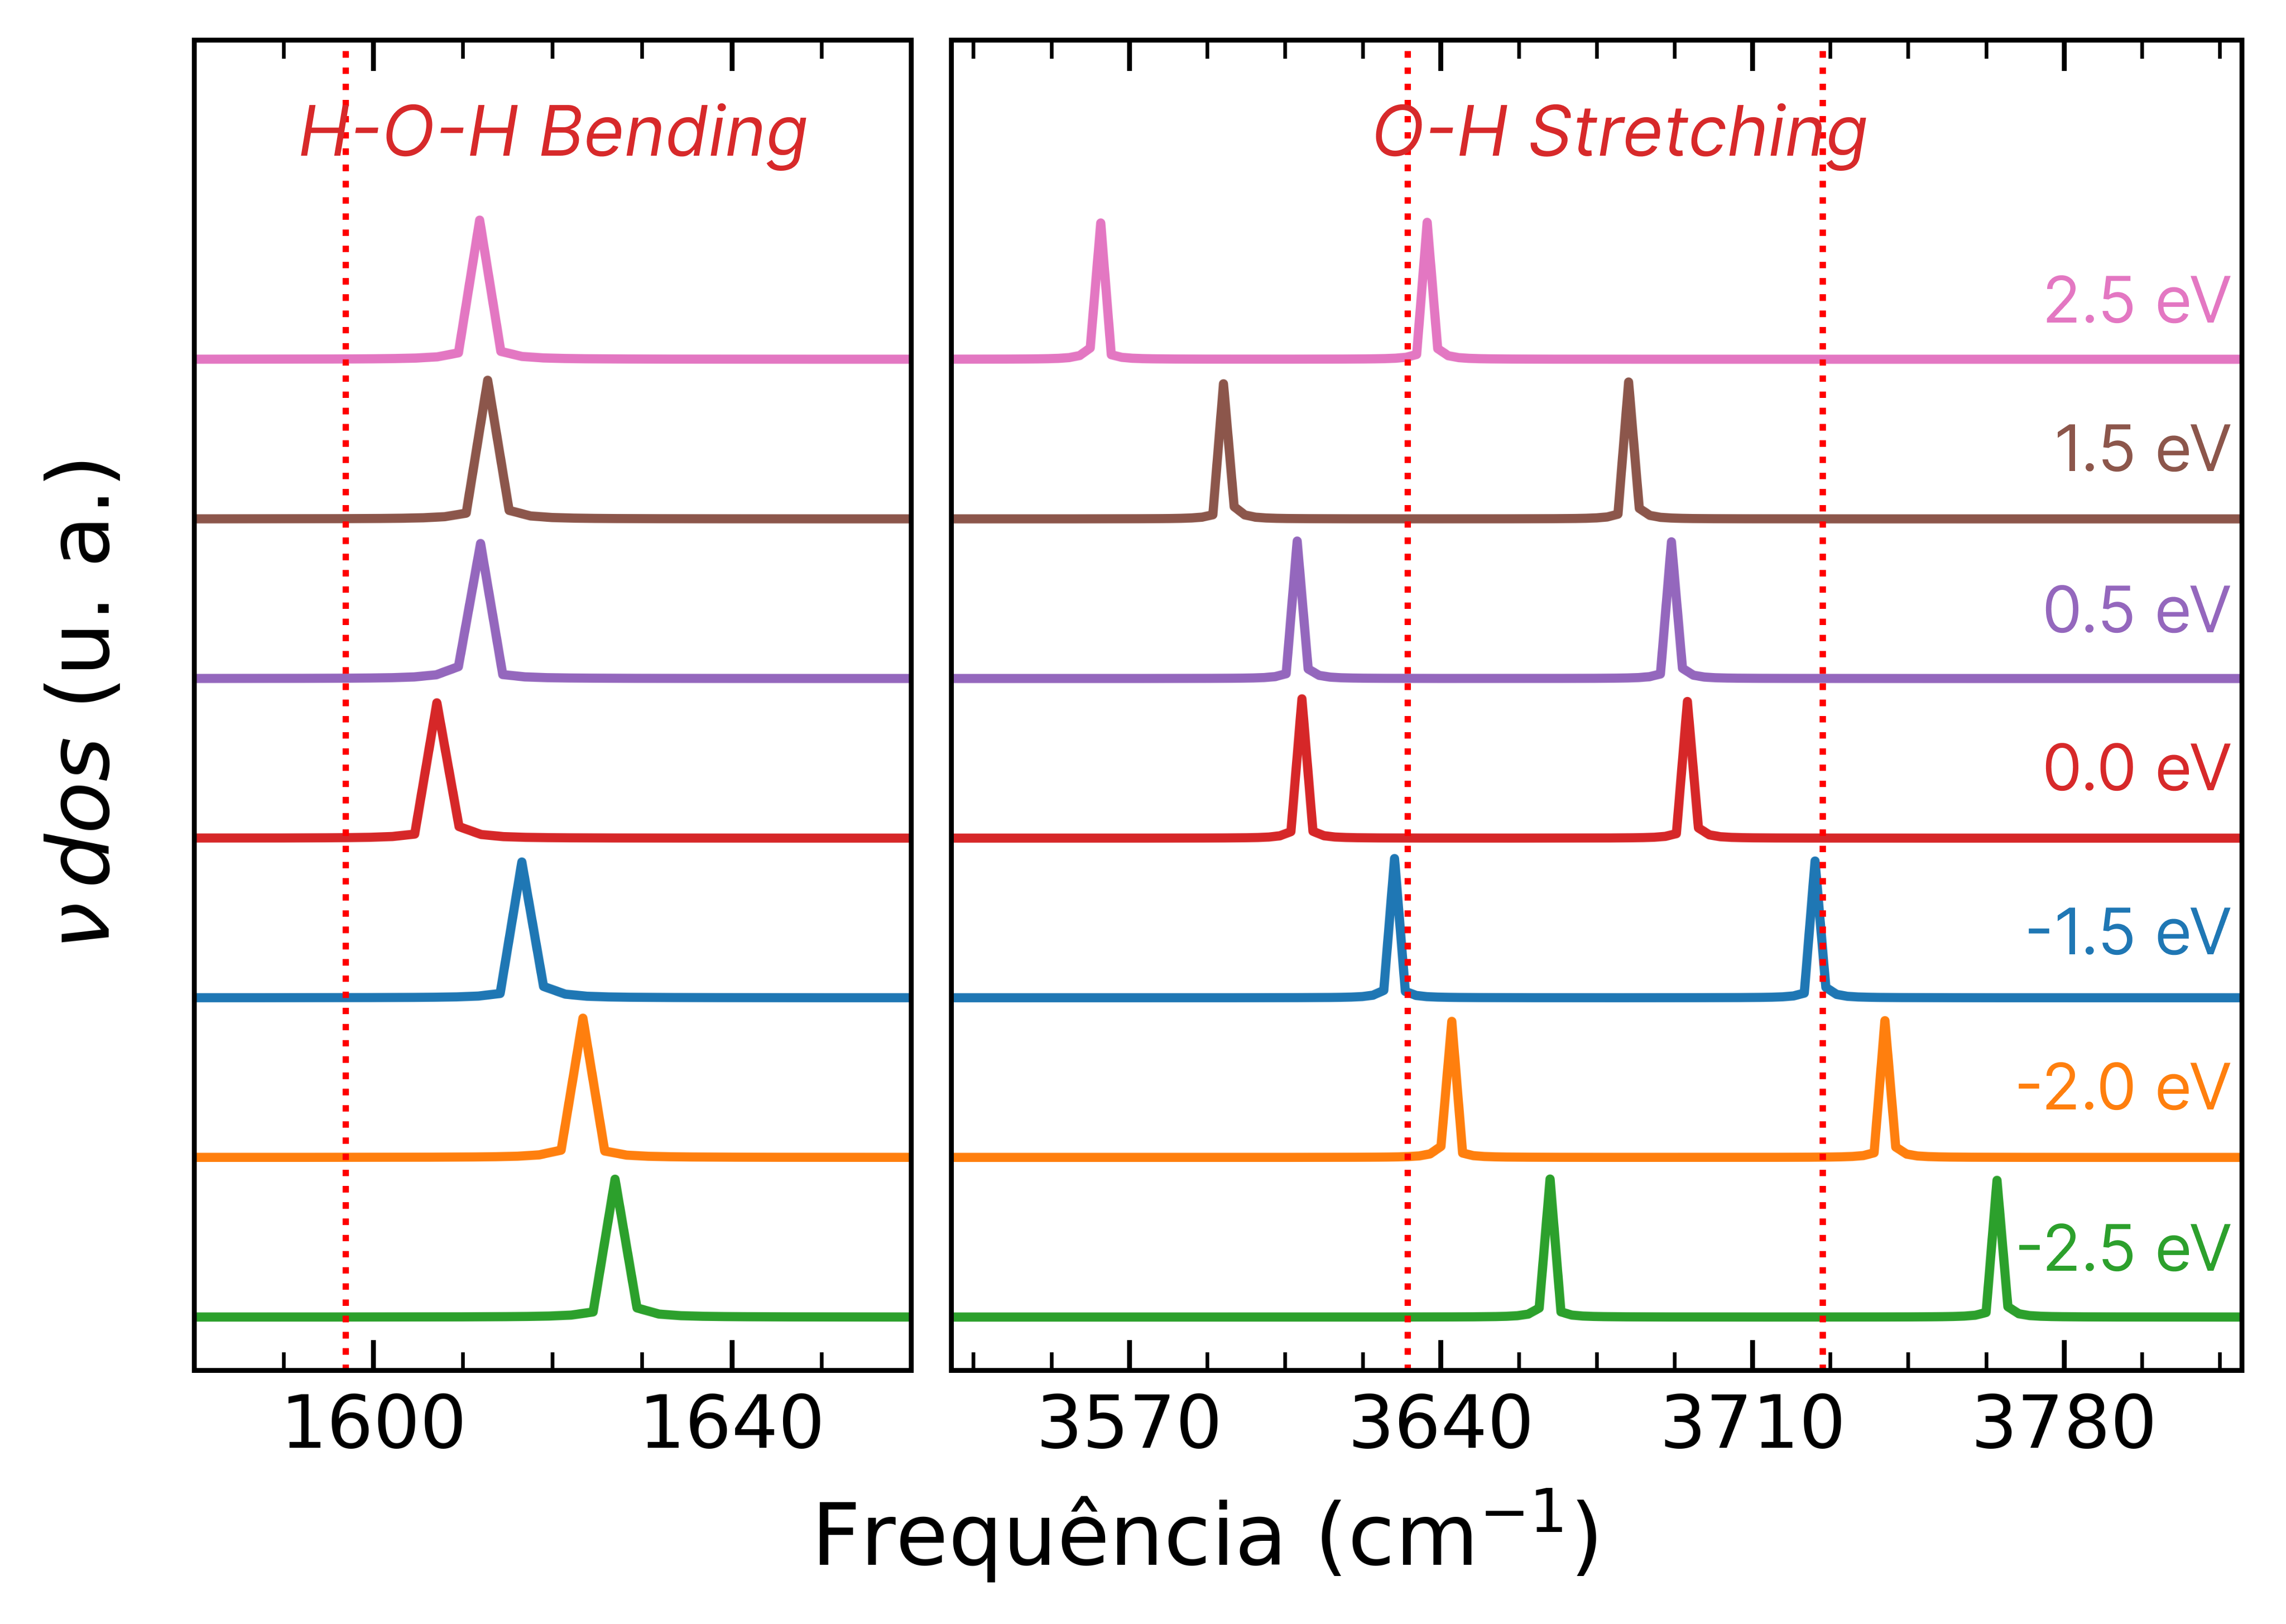
\includegraphics[scale=0.08]{figs/freq_monomer_pd.png}
	\legend{Fonte: compilação da autora.}
\end{figure}

As alterações estruturais provocadas pela diferença do potencial externo refletem nas frequências dos modos vibracionais (Tabela \ref{tab:neq_freq_pd} e Figura \ref{fig:neq_pd_mon_freq}). Tais alterações incluem a repulsão/atração da molécula de água em direção ao metal e o fato do eletrodo ser tratado como semi-infinito e não finito. Esse último ponto é visto pela diferença nas frequências obtidas com o sistema completo (Figura \ref{fig:sistema_pd}) com condições periódicas de contorno (\textit{periodic boundary conditions}- PBC), em relação ao slab de tamanho $ 6\times4\times4 $ camadas -- Tabela \ref{tab:modos}. Assim, houve uma diminuição média de $ \sim 75\;\si{\cm}^{-1} $ nas frequências de \textit{stretching} ao aumentar o número de camadas (4 para 10) e diminuir o tamanho do plano xy ($ 6\times4 $ para $ 3\times4 $). Essa variação é resultado do efeito eletrostático da molécula de água com as células vizinhas ao diminuir o tamanho da célula unitária, uma vez que ao tratar os eletrodos como semi-infinitos a variação foi de $ \sim 30\;\si{\cm}^{-1} $ nas frequências de \textit{stretching}. No entanto, devido ao custo computacional de um cálculo NEGF, aumentar o tamanho do plano metálico se torna inviável.  


Ao variar o potencial externo aplicado, as frequências diminuem com o aumento do potencial para V>0 variando $ 58\,\si{cm}^{-1} $ para $ V=2.5\,\si{\eV} $; quando o potencial diminuiu, as frequências aumentam até $ 70\,\si{cm}^{-1}$ para $ V=-2.5\,\si{\eV} $. Essas alterações refletem a rotação da molécula devido à superfície carregada, que por sua vez, intensificam ou enfraquecem as ligações O-H. Assim, para potenciais positivos, a molécula se liga mais fortemente ao metal através da interação entre os átomos de H e a superfície negativamente carregada. Por outro lado, para potenciais negativos, os átomos de H se afastam da superfície carregada positivamente e assim, interagem menos com o metal.

%Por fim, tem-se que a aplicação do potencial externo altera as propriedades estruturais e vibracionais da molécula adsorvida no Pd. Em particular 


O modelo estudado constitui um protótipo da interação água/metal e não inclui ligações de hidrogênio que são determinantes nas ativações de processos de oxidação e redução da molécula de água em superfícies metálicas carregadas \cite{bias-pd}. Além disso, através do cálculo de forças fora do equilíbrio foi possível realizar a otimização da geometria que determinou a posição de mínima energia e que revelaram alterações vibracionais e estruturais. Assim, não observou-se processos de oxidação ou redução do monômero na superfície metálica, pois essas reações resultam do balanço entre as interações da água com a superfície carregada e interações entre as moléculas de água da interface e as moléculas de água de camadas superiores \cite{pd_bias_exp,pd_bias_exp2,pd_bias_exp3}. %Assim, os resultados acima discutidos  ao se aplicar um potencial externo, todavia, não considerou o efeito sobre as ligações de hidrogênio. 

%Além disso, nossos resultados estão em concordância com resultados teóricos que revelaram o comportamento dependente do potencial das moléculas de água na superfície de Pd \cite{bias-pd}. Ademais, encontrou-se que o processo de redução ocorre através da dissociação da água e formação de hidretos na superfície e é ativado pela interação com o metal a 0.5 V. Por outro lado, a oxidação ocorre a 1.1 V através da formação de hidróxido na superfície e com transferência de prótons para as moléculas das camadas superiores. De acordo com os autores, a posição de equilíbrio da solução aquosa e processos de redução/oxidação resultam do balanço entre as interações da água com a superfície carregada e interações entre as moléculas de água da interface e as moléculas de água de camadas superiores. 
 



\section{Ouro\label{sec:au_negf}}

%Para a superfície metálica de Au(111) foram estudados dois sistemas protótipos: monômero e camada de água. O primeiro inclui apenas a interação água/metal (Seção \ref{sec:neq_au_mon}), ao passo que o segundo inclui tanto interações água/metal como ligações de hidrogênio entre água (Seção \ref{sec:neq_au_layer}).% Além disso, a camada representa um modelo da interface água líquida/metal. %Vale ressaltar que os eletrodos de Au(111) possuíam menos camadas que os eletrodos de Pd(111). Isso possibilitou estudar a camada de água adsorvida, bem como examinar o comportamento das estruturas com a aplicação de potenciais externos maiores, visto que um cálculo fora do equilíbrio é caro computacionalmente.
\subsection{Monômero \label{sec:neq_au_mon}}
A investigação do potencial externo aplicado à interface água/Au(111) iniciou pela análise do monômero na orientação \textit{flat} adsorvido na superfície metálica de Au(111) com $ 3\times4 $ átomos no plano da superfície. A base atômica localizada que descreve o Au é menor que a base utilizada no Pd (Apêndice \ref{apd:metal} -- Tabelas \ref{tab:raios_corte} e \ref{tab:au}) logo, o eletrodo utilizado possui 3 camadas e a região de espalhamento 4 e 3 camadas de cada lado (Figura \ref{fig:sistema_au}); o parâmetro de rede do Au utilizado foi de $ 4.24\,\si{\angstrom} $ e entre as duas superfícies metálicas havia um vácuo de $ 20\,\si{\angstrom} $, resultando em uma célula unitária de tamanho $ 10.30\times9.90\times53.00\,\si{\angstrom} $. Todas as minimizações foram realizadas com o funcional PBE e o potencial externo aplicado variou entre -5.0 a 5.0 eV, com intervalos entre 1.0 e 1.5 eV. %Para cada otimização, utilizou-se como coordenadas iniciais as obtidas com \textit{potencial 0}.
\begin{figure}[h!]
	\centering
	\caption{Ilustração do sistema utilizado para aplicar a diferença de potencial externa à interface água/Au(111), bem como as regiões correspondentes aos eletrodos e região de espalhamento.}
	\label{fig:sistema_au}
	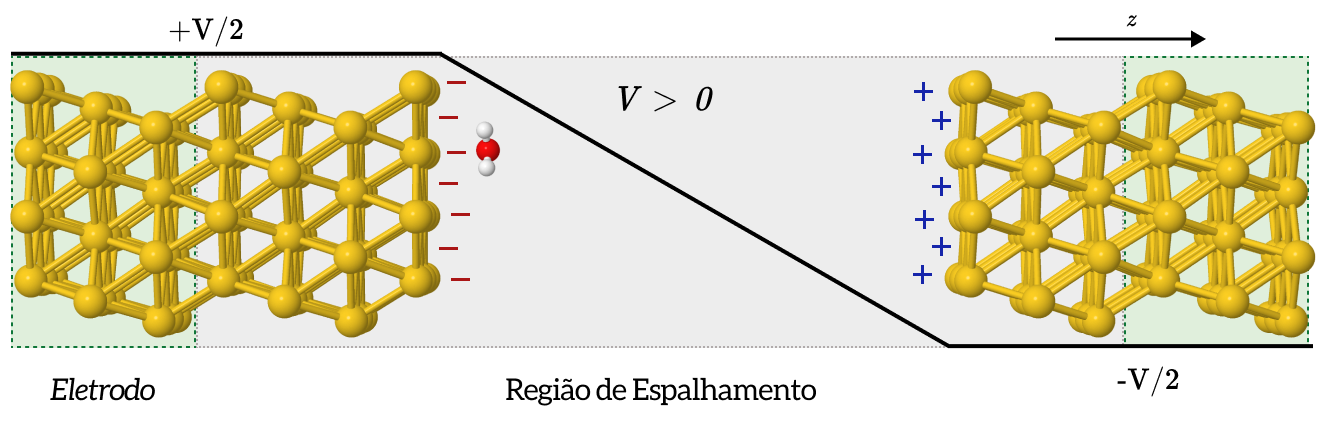
\includegraphics[scale=0.35]{figs/sistema_negf.png}
	\legend{Fonte: compilação da autora.}
\end{figure}

Utilizando condições periódicas de contorno, obteve-se que a energia de adsorção da molécula \textit{flat} adsorvida no Au foi de $ E_{ads-Au}=0.10\,\si{\eV}  $, próxima ao valor de 0.13 eV reportado na literatura com o funcional PW90 \cite{michaedelis}. Após a minimização com PBC obteve-se $d_{O-Au}=2.80\,\si{\angstrom} $ e $ \alpha=-8\si{\degree} $. Essa distância é maior que a distância do monômero adsorvido no Pd $ d_{O-Pd} =2.47 \,\si{\angstrom}$ e está de acordo com os valores obtidos com o \textit{potencial 0}($d_{O-Au}=2.82\,\si{\angstrom} $ e $ \alpha=-10\si{\degree} $). Assim, a molécula se liga fracamente ao Au, sendo portanto, reportado como um metal hidrofóbico \cite{monomer}. 

Analisando as propriedades geométricas da otimização do monômero em função do potencial externo para $ V\neq0 $ (Tabela \ref{tab:neq_au_geo} e Figura \ref{fig:neq_au_mon_geo}), observa-se uma variação significativa da distância a medida que se aumenta o valor de V, onde mesmo para o potencial V=1.5 eV a variação em relação à posição inicial foi de $ \Delta_{d_{O-Au}}=0.52\,\si{\angstrom} $. Em contrapartida, para esse mesmo potencial aplicado ao eletrodo de Pd a molécula se distanciou apenas $ 0.05 \,\si{\angstrom} $. Essa discrepância é resultado da hidrofobicidade do Au e da reatividade do Pd e revela o efeito desses fatores ao se aplicar um potencial externo numa célula eletroquímica.

 

\begin{table}[t!]
	\centering
	\caption{Propriedades geométricas obtidas a partir da otimização da molécula de água adsorvida na superfície metálica de Au(111) de acordo com o potencial V aplicado. As propriedades geométricas analisadas foram a distância entre o átomo de O e Au $d_{O-Au}(\si{\angstrom})$ e entre os átomos de H e de O $ d_{O-H}(\si{\angstrom})$, deslocamento lateral no eixo x e y ($ \Delta Oxy $), ângulo $ \Theta $ entre os átomos de H e inclinação $ \alpha $ em relação à superfície.\label{tab:neq_au_geo}}
	\begin{tabular}{Sccccc} 
		\hline\hline\addlinespace[3.6pt]
		\multicolumn{6}{c}{\textbf{Propriedades Geométricas $ H_2O/Au $ }}   \\\midrule
		{V (eV)}   &{$d_{O-Au}\,(\si{\angstrom}) $}&{$d_{O-H}\,(\si{\angstrom}) $} &{$\Delta\, Oxy \, (\si{\angstrom})$}	&{$\Theta(\si{\degree})$}&{$\alpha(\si{\degree})$}\\
		\hline
		5.0		&3.55	&0.98	&1.56	&101	&-89\\	
		4.0		&3.57	&0.98/0.97	&1.67	&102	&-90\\	
		2.5		&3.49	&0.97	&1.53	&102	&-87\\
		1.5		&3.34	&0.98/0.97	&1.34	&102	&-73\\
		0.0		&2.82	&0.97	&0.49	&104	&-10\\
		-1.5		&2.72	&0.97	&0.07	&104	&25 \\
		-2.5		&2.70	&0.97	&0.13	&104	&36 \\
		-4.0		&2.71	&0.97	&0.28	&104	&53 \\
		-5.0		&2.72	&0.97	&0.48	&104	&66 \\ %\midrule 
	%	PBC		&2.80	&0.97	&0.48	&104	&-8 \\
		\hline\hline
	\end{tabular}
	\legend{Fonte: compilação da autora.}
\end{table}


\begin{figure}[b!]
	\centering
	\caption{Variação da inclinação $ \alpha $ e da distância $ \Delta d_{O-Au} $ em função do potencial externo aplicado V. A distância $ \Delta d_{O-Au}=d_{O-Au,V}-d_{0}$ é medida em comparação à posição inicial $ d_0=2.82\;\si{\angstrom} $. No gráfico também estão ilustrados as posições finais do monômero após otimização para cada potencial.}
	\label{fig:neq_au_mon_geo}
	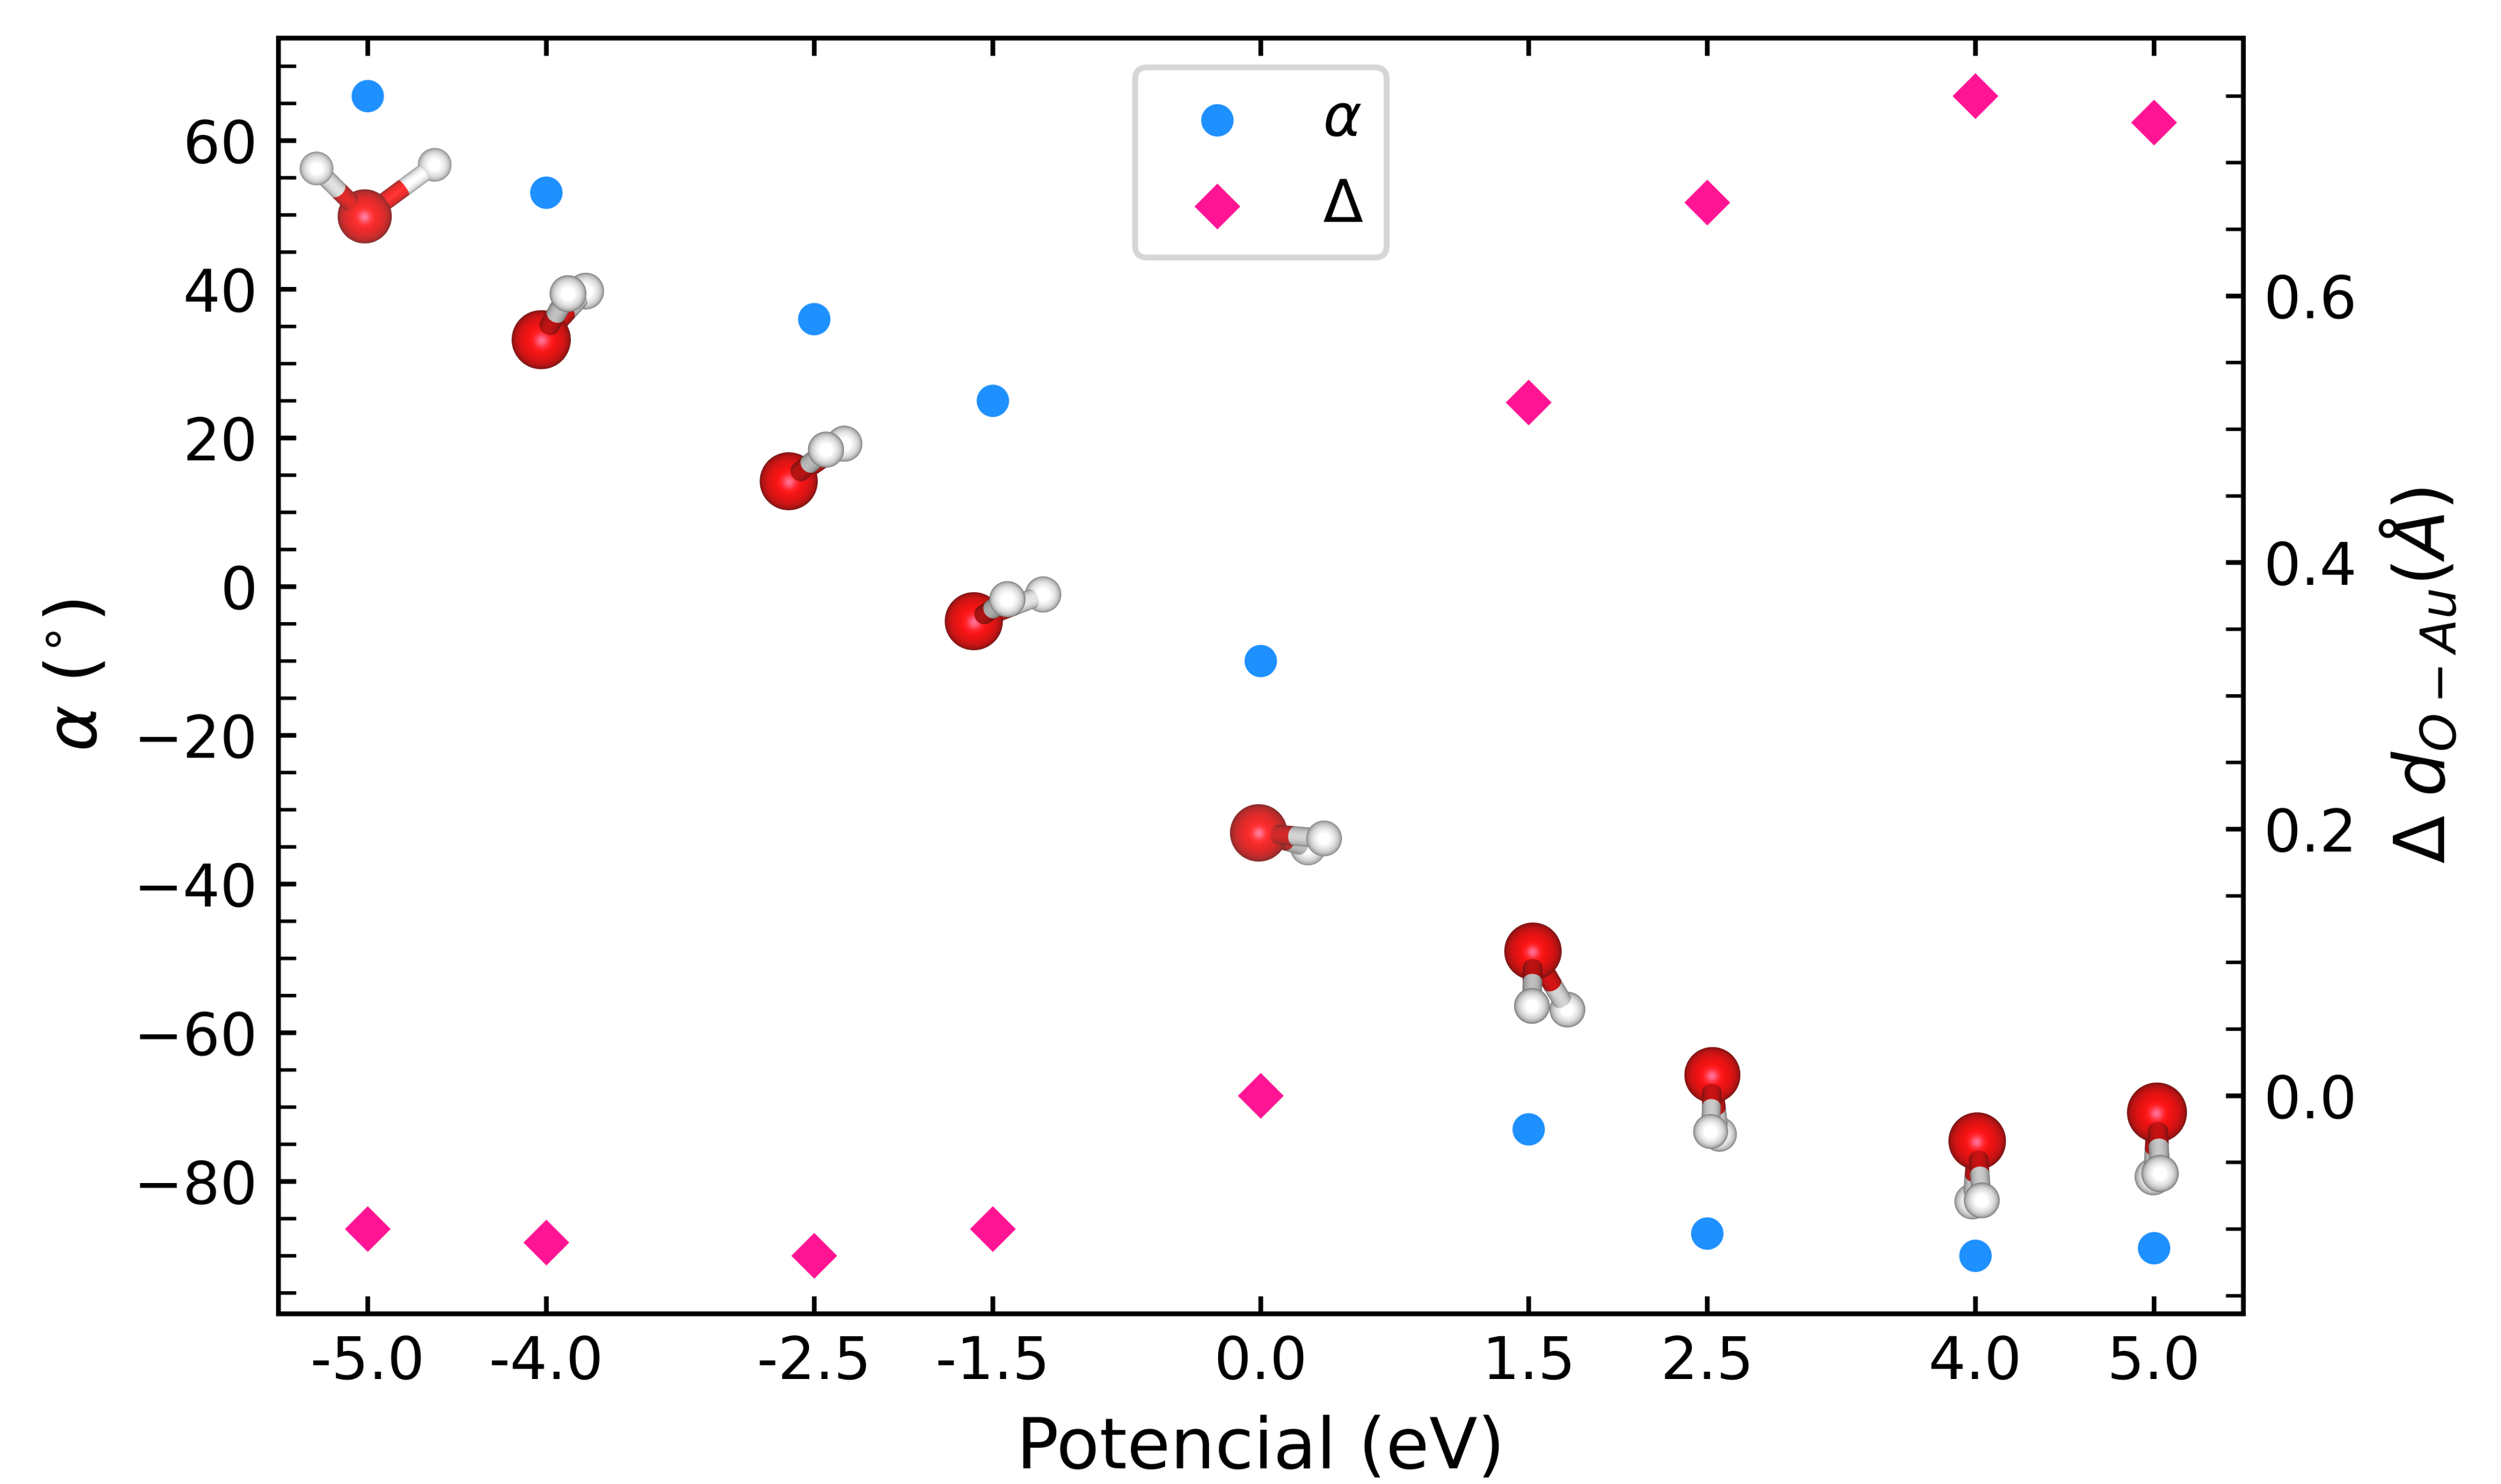
\includegraphics[scale=0.09]{figs/ang_monomer.jpg}
	\legend{Fonte: compilação da autora.}
\end{figure}

Ademais, observa-se que para $ V>2.5 \,\si{\eV} $, a inclinação da molécula $ \alpha $ praticamente não muda, ao passo que a variação da distância inicial muda progressivamente até 4.0 eV e depois apresenta um decréscimo. Esse efeito é resultado da polarização superficial do metal, no qual para potenciais positivos o átomo de oxigênio é repelido e os átomos de hidrogênio são atraídos; logo, a molécula fica na orientação \textit{down}. Para potenciais negativos observa-se o comportamento contrário, onde a variação da distância se mantém constante e com valor de $\Delta_{d_{O-Au}}= -0.1 \,\si{\angstrom} $ e as alterações ocorrem na inclinação em relação à superfície metálica; assim, a orientação da molécula se torna \textit{up}. De modo geral, percebe-se um comportamento padrão da molécula a partir de um determinado potencial: para potenciais positivos isso ocorre na inclinação e para os negativos na distância $ d_{O-Au} $.  

Como observado anteriormente, a aplicação do potencial altera também a reatividade do metal. No caso do Au, o potencial positivo intensifica o caráter hidrofóbico, fazendo com que a molécula se afaste mais do metal e também do sítio de adsorção \textit{atop}; isso é visto pelo aumento nas medidas $ d_{O-Au} $ e $ \Delta Oxy $. Em relação às propriedades intramoleculares, observa-se um alargamento do ângulo $ \Theta $ para os potenciais negativos e uma diminuição para os potenciais positivos. Assim como no Pd, as modificações estruturais são assimétricas e dependem do sinal do potencial aplicado. % Por outro lado, para o potencial negativo $ V=-1.5\,\si{\eV} $ a molécula se encontra acima do átomo de Au. 
 \begin{figure}[b!]
	\centering
	\caption{(a) Diferenças de densidades de carga $ \Delta \rho_{V} $ em relação ao potencial de 0.0 eV para os potenciais 1.5, 2.5 e 5.0 eV, cujos valores de isosuperfícies correspondem a $ 3.57\times10^{-4}\;\si{e}/\si{\angstrom}^3 $. Na última coluna estão representados as flutuações de densidades de carga com os respectivos valores de isosuperfícies $ 1.11\times10^{-5}$, $ 1.71\times10^{-5}$ e $ 5.57\times10^{-5}\;\si{e}/\si{\angstrom}^3 $. Em todos os casos, azul (vermelho) indica uma deficiência (excesso) de elétrons. (b) Gráfico das diferenças de densidades de carga média ao longo do eixo z de acordo com o potencial aplicado V.}
	\label{fig:neq_au_mon_dens}
	\includegraphics[scale=0.067]{figs/dens_bias-monomer.png}
	\legend{Fonte: compilação da autora.}
\end{figure}


O efeito de atração/repulsão da molécula de água pode ser visto por meio dos gráficos de diferença de densidade de carga $ \Delta\rho_V $ (Figura \ref{fig:neq_au_mon_dens} (a)). No gráfico, vemos uma maior concentração de carga no átomo de oxigênio e na superfície metálica. Essa concentração é proporcional ao aumento do potencial e possui um comportamento assimétrico entre o potencial positivo e negativo ($ \Sigma\Delta\rho_{_ {V}} $). Por meio do gráfico de flutuação média de carga ao longo do eixo z (Figura \ref{fig:neq_au_mon_dens} (b)), observa-se uma variação de densidade de carga na região da molécula e na última camada metálica; essas variações indicam transferência de carga entre a molécula e o metal. Portanto, a posição de equilíbrio do monômero para um dado valor de V é resultado da transferência de carga, interação eletrostática e repulsão de Pauli \cite{artigo-luana}.   

Após analisar como as interações e as propriedades estruturais são afetadas pelo potencial, investigamos os modos normais de vibrações da molécula de água (Tabela \ref{tab:neq_au_mon_freq}). Para a otimização realizada com PBC as frequências de \textit{bending} foi de $ 1642\,\si{\cm}^{-1} $ e as de \textit{stretching} simétrico e assimétrico foram $ 3644\,\si{\cm}^{-1}$ e $ 3758\,\si{\cm}^{-1} $, respectivamente. Comparando esses valores com os obtidos utilizando o formalismo de NEGF a V=0.0 eV, vemos que os valores são similares. Vale notar que as frequências de \textit{stretching} do monômero adsorvido no Au são superiores às frequências do Pd com o \textit{potencial 0}. Isso está relacionado ao fato da molécula estar mais afastada do Au em relação ao Pd e às propriedades de reatividade de cada superfície. 
 \begin{table}[t!]
	\centering
	\caption{Frequências dos modos normais de vibrações do monômero adsorvido no Au(111) de acordo com o potencial externo V aplicado.\label{tab:neq_au_mon_freq}}
	\begin{tabular}{Sccc} 
		\hline\hline\addlinespace[3.6pt]
		\multicolumn{4}{c}{\textbf{Frequências dos Modos Normais $ H_2O/Au\,(\mathbf{\si{\cm}^{-1}})$}}\\ \midrule
		{V (eV)}   &$Bending$	&$\textit{Stretching} \, (S)$	&$\textit{Stretching} \, (AS)$\\
		\hline
		5.0		&1642	&3597	&3687\\
		4.0		&1639	&3613	&3685\\	
		2.5		&1630	&3618	&3704\\	
		1.5		&1623	&3602	&3697\\
		0.0		&1626	&3646	&3759\\
		-1.5		&1624	&3675	&3790\\
		-2.5		&1630	&3671	&3798\\
		-4.0		&1638	&3673	&3797\\
		-5.0		&1647	&3653	&3789\\ %\midrule
	%	PBC		&1624	&3644	&3758 \\
		\hline\hline
	\end{tabular}
	\legend{Fonte: compilação da autora.}
\end{table}


\begin{figure}[h!]
	\centering
	\caption{Distribuições das densidades de estados vibracionais (unidades arbitrárias) de acordo com potencial externo aplicado na interface monômero/Au. As distribuições estão divididas de acordo com os modos fundamentais do monômero \textit{bending}, \textit{stretching} e translacionais. As linhas tracejadas representam os valores experimentais do monômero isolado.}
	\label{fig:neq_au_mon_freq}
	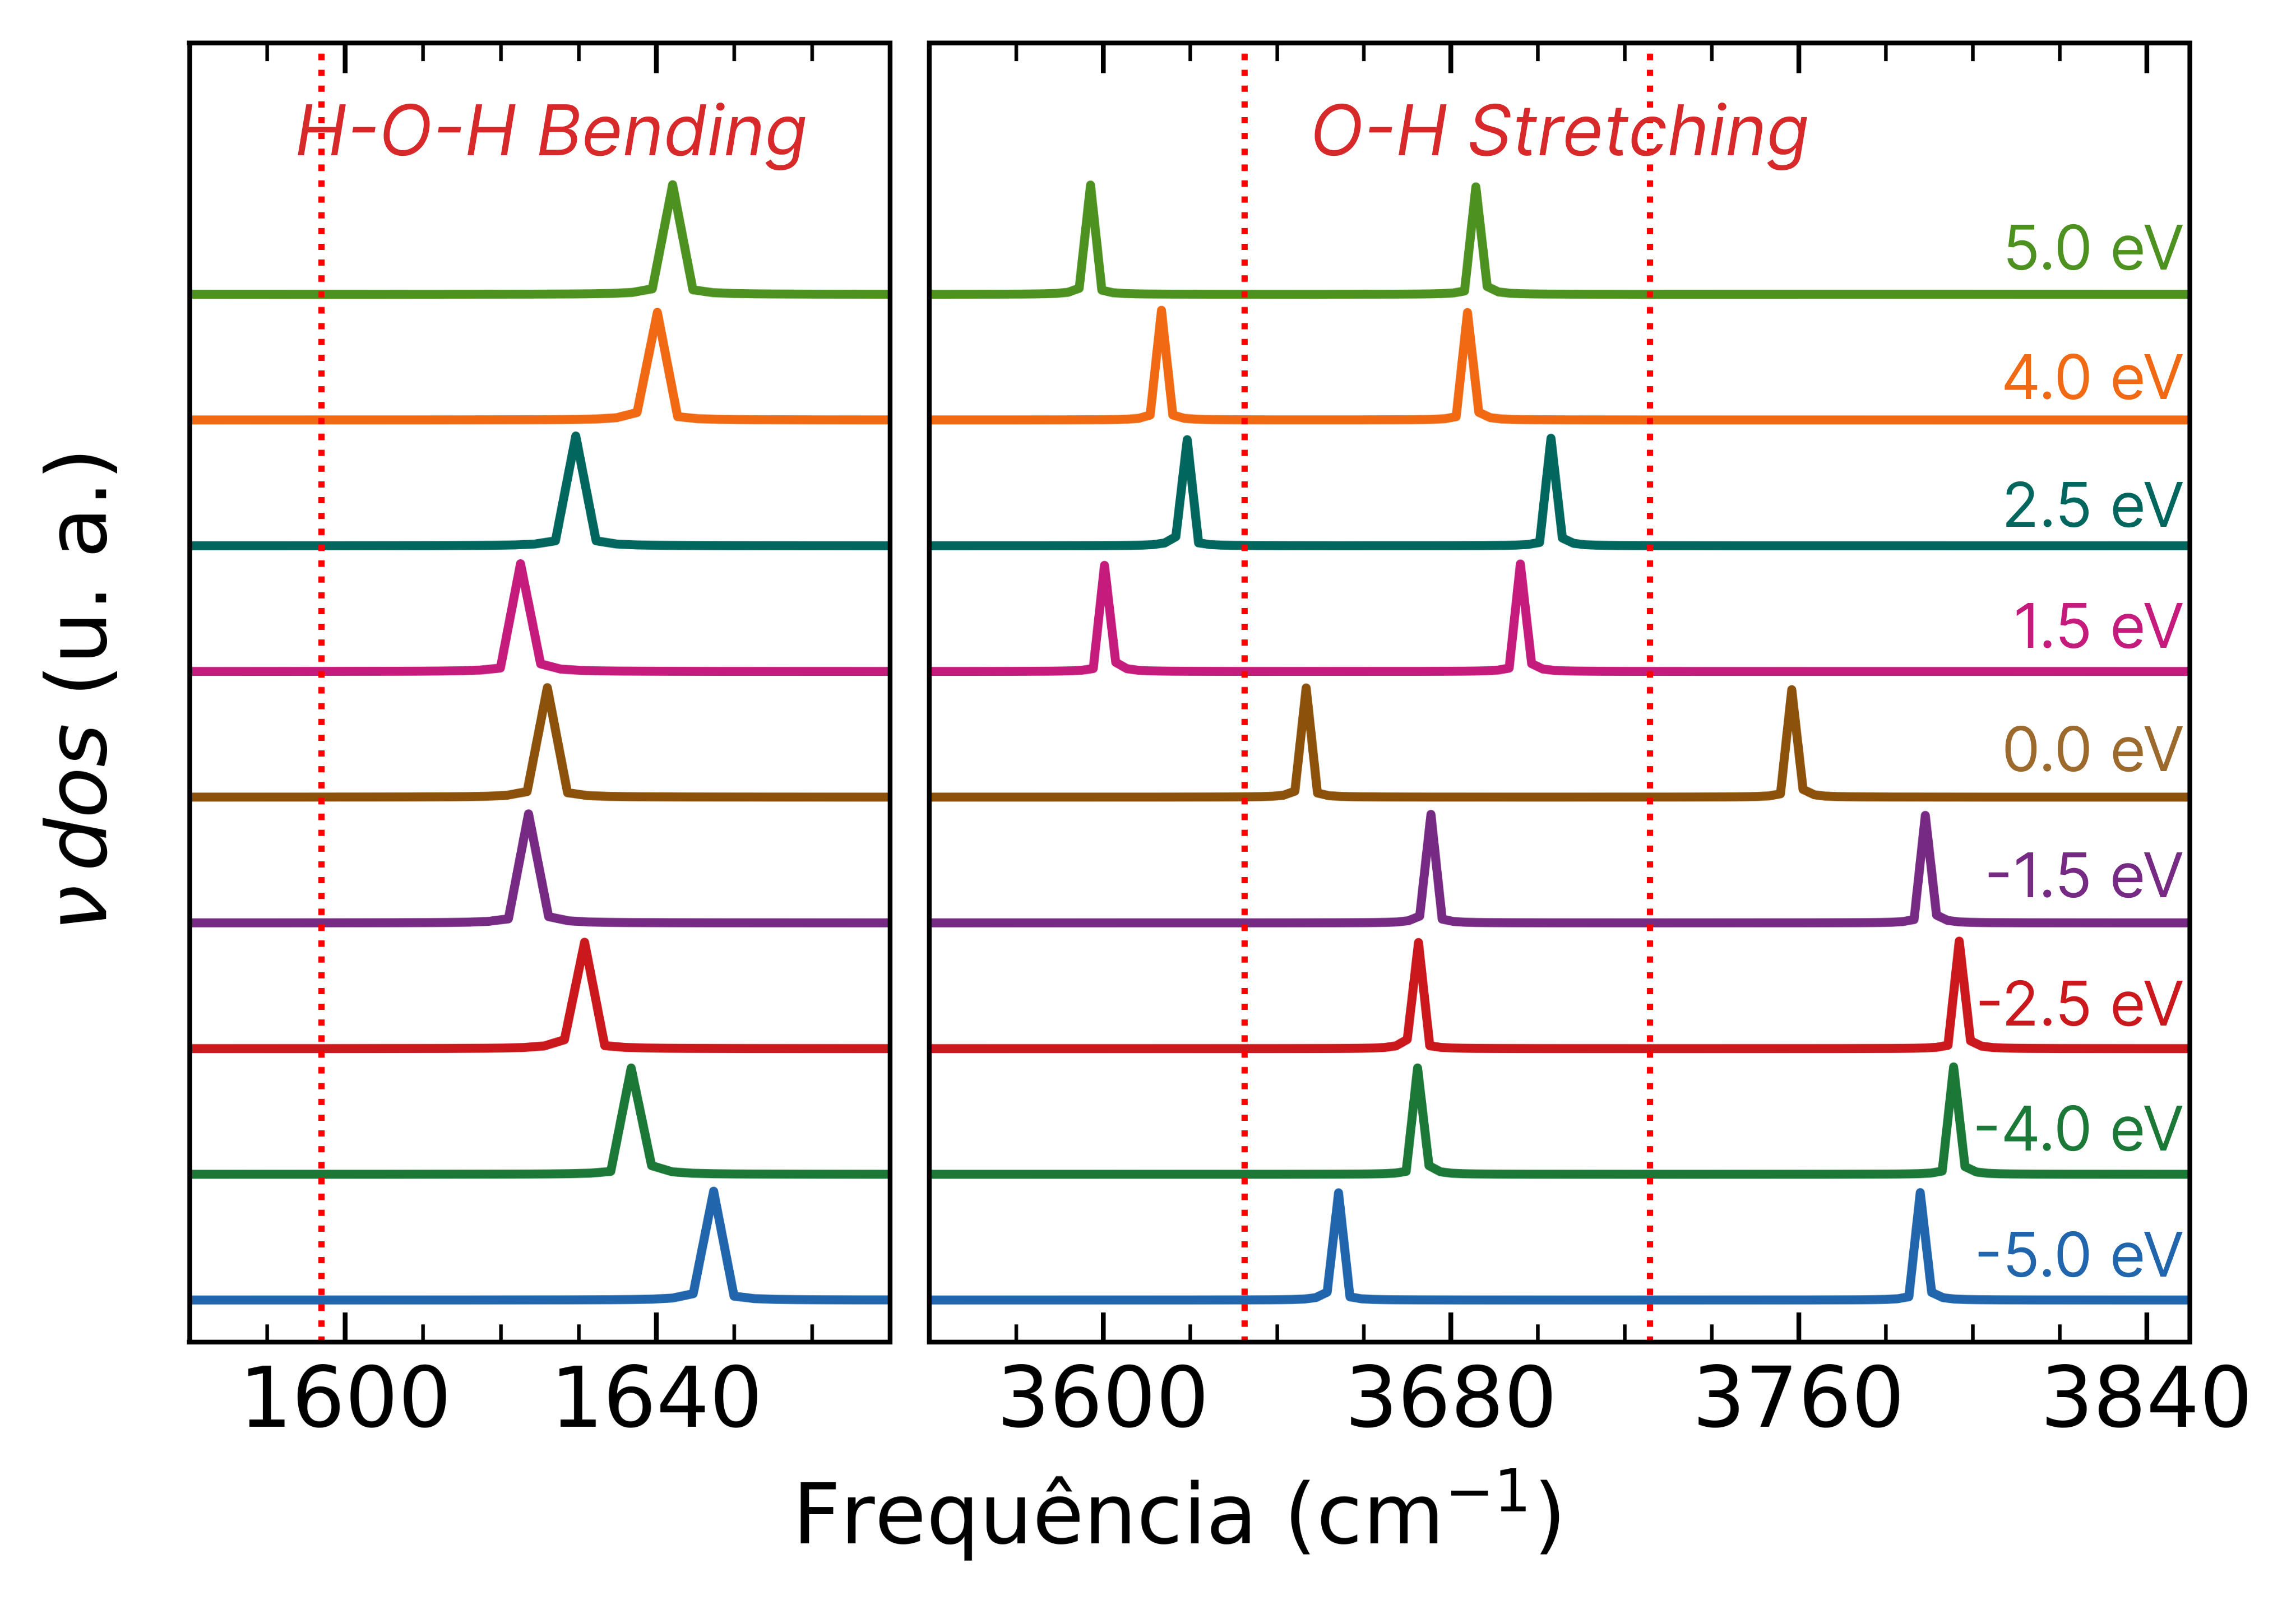
\includegraphics[scale=0.08]{figs/freq_monomer_au.png}
	\legend{Fonte: compilação da autora.}
\end{figure}


Para os potenciais negativos observa-se que a frequências de \textit{stretching} antissimétrico aumenta $ 31\,\si{\cm}^{-1} $ e depois se mantém praticamente constante; por outro lado, para a frequência de \textit{stretching} simétrico, observa-se um aumento de $ 29\,\si{\cm}^{-1} $ e em seguida uma redução nas frequências. Esse aumento das frequências está associado a menor interação das ligações O-H com o metal devido à rotação das moléculas na direção contrária à superfície. Para V>0, observa-se uma tendência de redução nas frequências de \textit{stretching} por causa da maior proximidade das ligações O-H com o metal,no qual a redução máxima do \textit{stretching} simétrico foi de $ 49\,\si{\cm}^{-1} $ e do assimétrico $ 74\,\si{\cm}^{-1} $. 

Com o intuito de investigar se a aplicação do potencial sobre o monômero era reversível e identificar possíveis transições de fases, foi realizado a otimização da estrutura através de  voltametria cíclica -- Figura \ref{fig:neq_au_voltametria} (c). Nas otimizações descritas anteriormente, as coordenadas iniciais das relaxações eram as obtidas a partir da relaxação do \textit{potencial 0}. No processo de voltametria, utilizava-se as coordenadas finais da relaxação a V=5.0 eV para realizar a otimização a $ V=4.0\,\si{\eV}$; isso era feito progressivamente até atingir $ V=5.0\,\si{\eV}$ (sentido negativo). O mesmo foi feito para $ V=-5.0\,\si{\eV}$ até atingir $ V=5.0\,\si{\eV}$ (sentido positivo). Em seguida, para cada otimização era calculado os modos normais de vibrações, onde as frequências de \textit{stretching} estão representadas na Figura \ref{fig:neq_au_voltametria} (a) e (b). 

%\todo[inline,color=green!40]{Falar um pouco mais sobre os resultados experimentais.}

Assim, o que se observa é que para as frequências de \textit{stretching} simétrico e assimétricos, as curvas do sentido positivo e negativo seguem a mesma tendência e apresentam variações dentro da margem de erro. Portanto, os diferentes processos pelos quais se aplica a variação do potencial são equivalentes. Por outro lado, experimentalmente observa-se processos de oxidação e redução na superfície metálica ao realizar a voltametria cíclica que são observados a partir das alterações nas frequências vibracionais \cite{sfg_kramer}. De acordo com \citeauthor{sfg_kramer}, esses processos estão relacionados ao efeito da superfície carregada sobre as moléculas de água e também devido às interações entre as moléculas da interface com as moléculas da água \textit{bulk}. 

\begin{figure}[h!]
	\centering
	\caption{(a) Frequências de \textit{Stretching} simétrico e (b) assimétrico do monômero adsorvido no Au(111) obtidas na voltametria cíclica, respectivamente. (c) Esquema da aplicação do potencial externo sobre o sistema na voltametria cíclica.}
	\label{fig:neq_au_voltametria}
	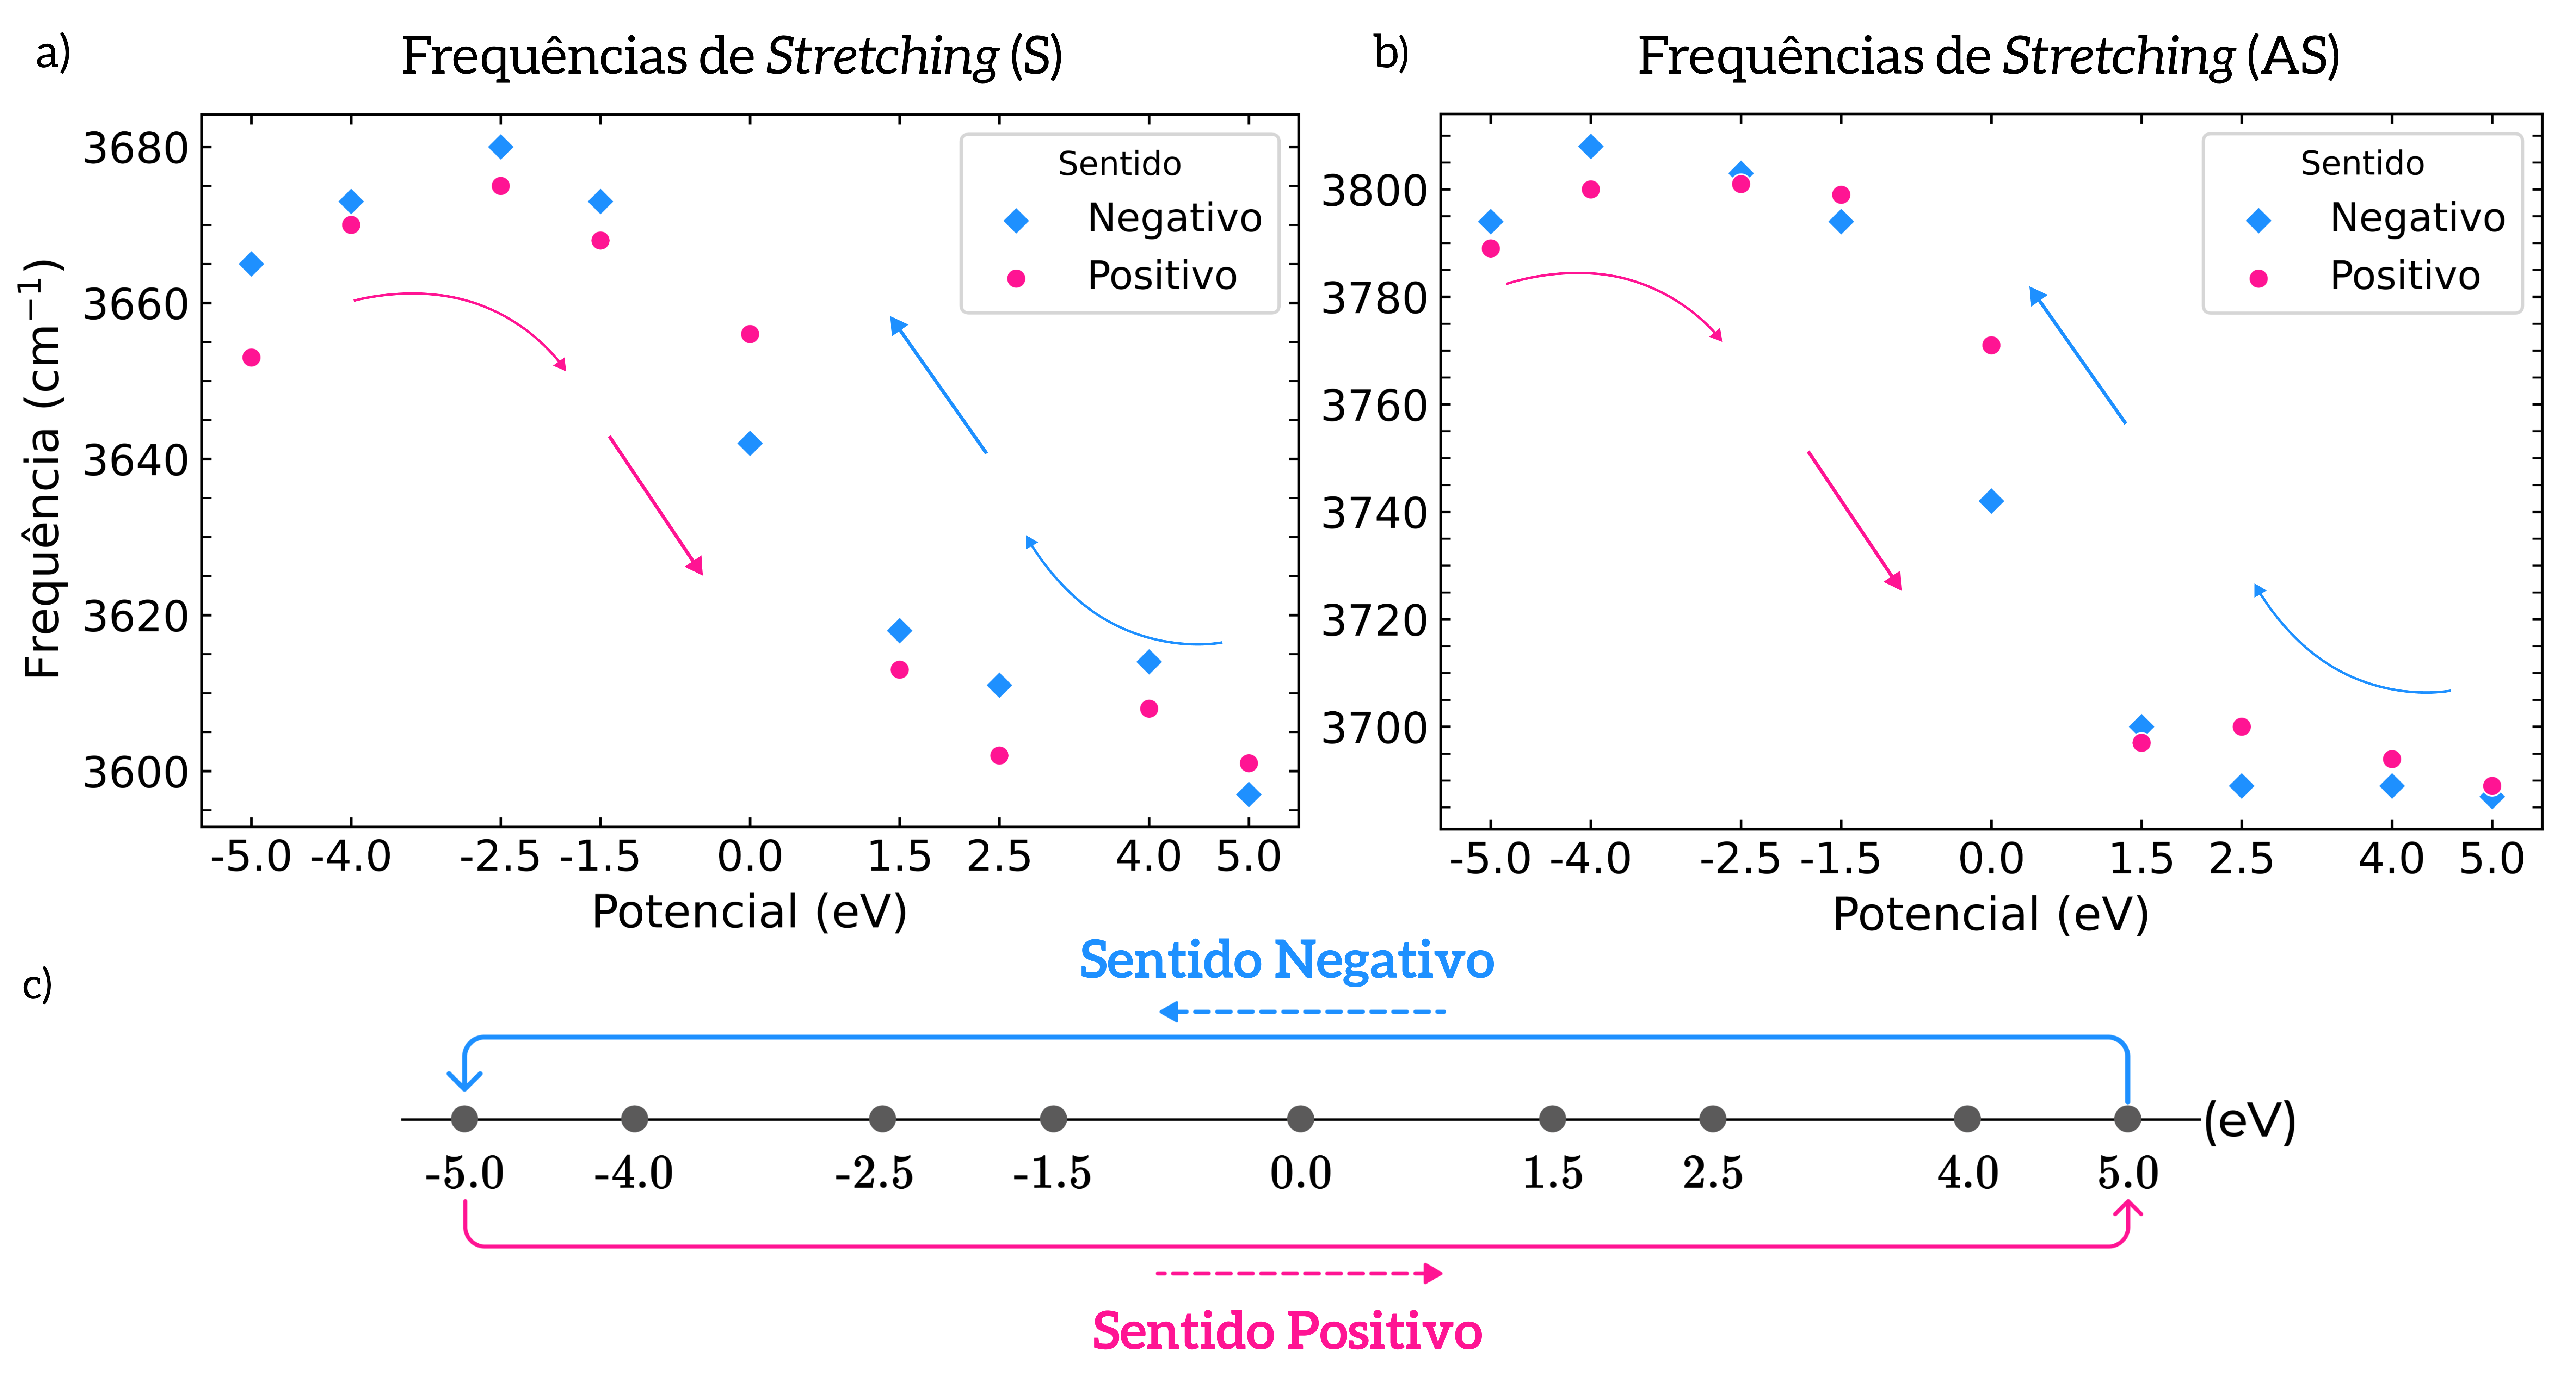
\includegraphics[scale=0.06]{figs/voltametria_monomer.png}
	\legend{Fonte: compilação da autora.}
\end{figure}

\subsection{Camada de Água \label{sec:neq_au_layer}}

Após caracterizar a interação água/metal sob a influência do potencial externo, investigamos como as ligações de hidrogênio são afetadas. Para isso, aplicamos um potencial externo sobre uma camada do tipo \textit{H-Down} adsorvida numa superfície metálica de Au(111) (Figura \ref{fig:neq_au_geo_layer}). Essa camada foi escolhida, pois resultados teóricos utilizando cálculos de DFT a mostraram como mais estável \cite{monomer}. 

No entanto, no âmbito experimental, a orientação exata da molécula de água na interface com o metal ainda é indefinida, principalmente considerando um potencial externo sobre o sistema. Nesse sentido, no estudo experimental conduzido por \citeauthor{sfg_kramer} foi observado alterações vibracionais ao aplicar uma variação de potencial na interface água/Au (111), as quais foram associadas às modificações estruturais. De acordo com os autores, os resultados indicam ligações O-H apontando para o metal (\textit{dangling OH-bonds}) no potencial de carga zero, de forma que, ao aplicar a diferença de potencial essas ligações são atraídas para a superfície metálica quando o potencial é negativo ou repelidas para potenciais positivos. Esse comportamento também foi observado em simulações computacionais, onde \citeauthor{pd_bias_layer} examinaram a adsorção de uma camada de água no Pd(111) e encontraram transição de fase de primeira ordem a partir de um determinado potencial através do cálculo da energia livre. Os autores associaram essa transição à mudança de orientação das moléculas de \textit{flat-down} para \textit{flat-up}.
\begin{table}[b!]
	\centering
	\caption{Propriedades geométricas médias da Camada de água adsorvida no Au (111) de acordo com o potencial externo V aplicado. As distâncias analisadas foram tomadas em relação aos valores médios das moléculas nas orientações \textit{flat-down} e \textit{flat} e correspondem a: distâncias entre os átomos de O ($ {d_{OO}} $), distâncias entre os átomos de O e Au ${d_{O-Au}}(\si{\angstrom})$, inclinação $ \alpha $ em relação à superfície, distância entre os átomos de H e O $ {d_{O-H}}(\si{\angstrom})$, onde o primeiro valor corresponde à ligação OH com o metal e segundo à ligação de hidrogênio, além do ângulo médio $ \Theta $ entre os átomos de H.}
	\begin{tabular}{Scccccccccc} 
		\hline\hline\addlinespace[3.5pt]
		\multicolumn{11}{c}{\textbf{Propriedades Geométricas ($ \si{\angstrom} $) -- Camada de Água/Au(111)}}  \\                                                                                                 
		\midrule
		{\multirow{2}{*}{{V(eV)}}}                                                                                                    & \multicolumn{2}{c}{${d_{OO}}$} & \multicolumn{2}{c}{\textbf{${d_{O-Au}}$}} &  \multicolumn{2}{c}{$\alpha$}& \multicolumn{2}{c}{\textbf{${d_{O-H}}$}}& \multicolumn{2}{c}{$\Theta$} \\ 
		\cmidrule{2-11}      &$ {d_{OO1}} $ &$ {d_{OO2}} $                  & \textit{Down}  & \textit{Flat}	&\textit{Down}  &\textit{Flat}	&\textit{Down}  &\textit{Flat}  &\textit{Down}  &\textit{Flat}   \\
		\midrule
		-5.00 & 2.97&3.02 &3.31  &2.93&-39  &28 	 &$0.98\,/ \, 0.99$  &$0.98$&102  &105     \\
		-4.00 &2.96&3.03 & 3.31  &2.96	 &-40  &26   &$0.98\,/ \, 0.99$  &$0.98$	&  102  &105    \\
		-2.50 &3.93&3.04 & 3.32  &3.03 &-41  &24  	 &$0.98\,/ \, 0.99$  &$0.98$	&  102  &105      \\
		-1.50 &2.92&3.04 & 3.33  &3.09	 &  -42  &21  &$0.98\,/ \, 0.99$  &$0.98$	&  102  &105     \\
		0.00 &2.90&3.05 & 3.35  &3.18	&  -42  &18  &$0.98\,/ \, 0.99$  &$0.98$	&  102  &106     \\
		1.50 &2.89&3.05 & 3.37  &3.29&  -43  &14 	  &$0.98\,/ \, 0.99$  &$0.98$	&  102  &106     \\
		2.50 &2.88&3.06 & 3.37  &3.35  &-43  &10	&  $0.98\,/ \, 0.99$  &$0.98$	&  102  &106     \\
		4.00 &2.88&3.07 & 3.41  &3.58&-42  &0  	&  $0.98\,/ \, 0.99$  &$0.98$	&  102  &106      \\
		5.00 &2.88&3.09 & 3.44  &3.75	&  -41  &-7   &$0.98\,/ \, 0.99$  &$0.98$	&  103  &106    \\ \midrule
	%	PBC && & 3.34  &3.13	&  0.98  &0.98	&  102  &105   &-42  &19   \\
		\hline\hline 
	\end{tabular}
	\legend{Fonte: compilação da autora.}
\end{table}

\begin{figure}[h!]
	\centering
	\caption{(a)Variação média da inclinação $ \alpha $ e da distância inicial $ \Delta d_{O-Au} $ das moléculas \textit{flat} de acordo com o potencial. A variação da distância $ \Delta d_{O-Au}= d_{O-Au,V}-d_{0}$ foi determinada em relação à posição inicial média $ d_0=3.18\,\si{\angstrom}$ obtida após a relaxação com o \textit{potencial 0}. Abaixo, a posição das moléculas \textit{flat-down} e \textit{flat} foi ilustrada para diversos potenciais e ao lado está representado as medidas representadas no gráfico. (b) Variações das distâncias médias $ d_{OO1} $ e $ d_{OO2} $ entre os átomos de O de acordo com o potencial aplicado.}
	\begin{subfigure}{0.9\textwidth}            
		\caption{\textit{Variações de $ \alpha $ e $ \Delta d_{O-Au} $das moléculas \textit{flat}}.}
		\centering
		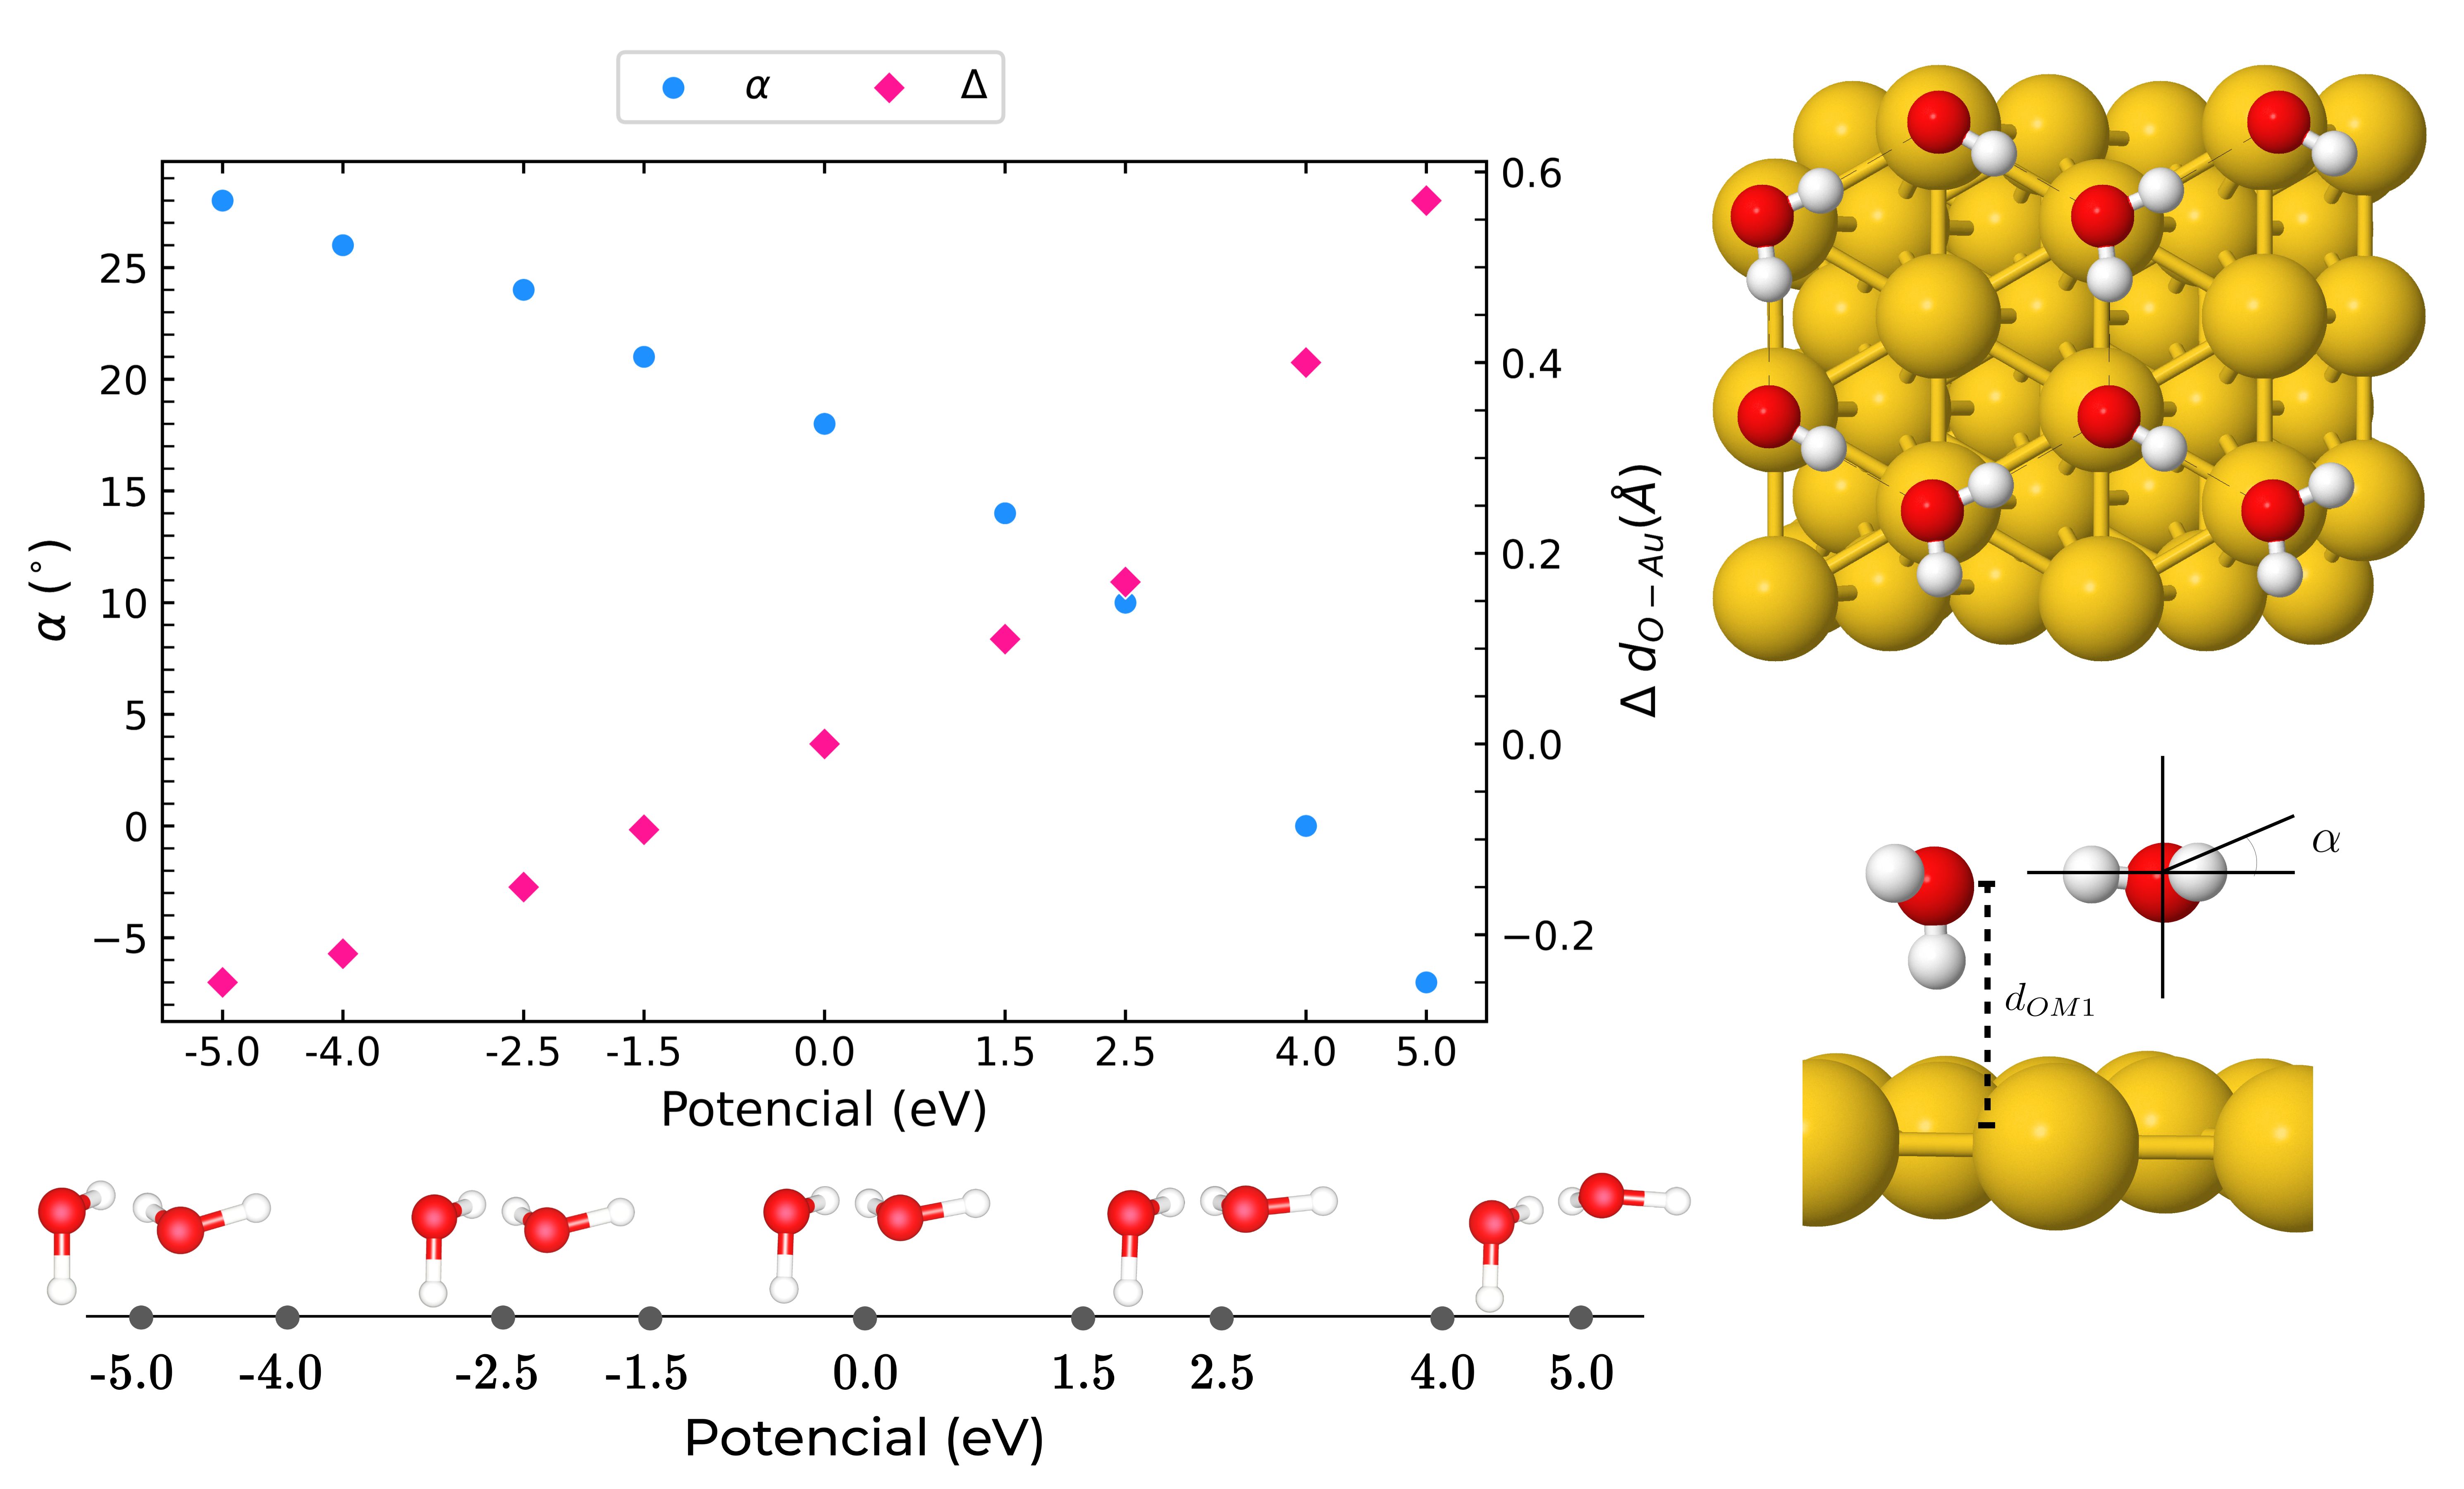
\includegraphics[width=\textwidth]{figs/ang_layer.png}
		\legend{Fonte: compilação da autora.}
		\label{fig:neq_au_geo_layer}
	\end{subfigure}\,
	\begin{subfigure}{0.7\textwidth}
		\caption{\textit{Variações das distâncias $ d_{O-O} $.}}
		\centering
		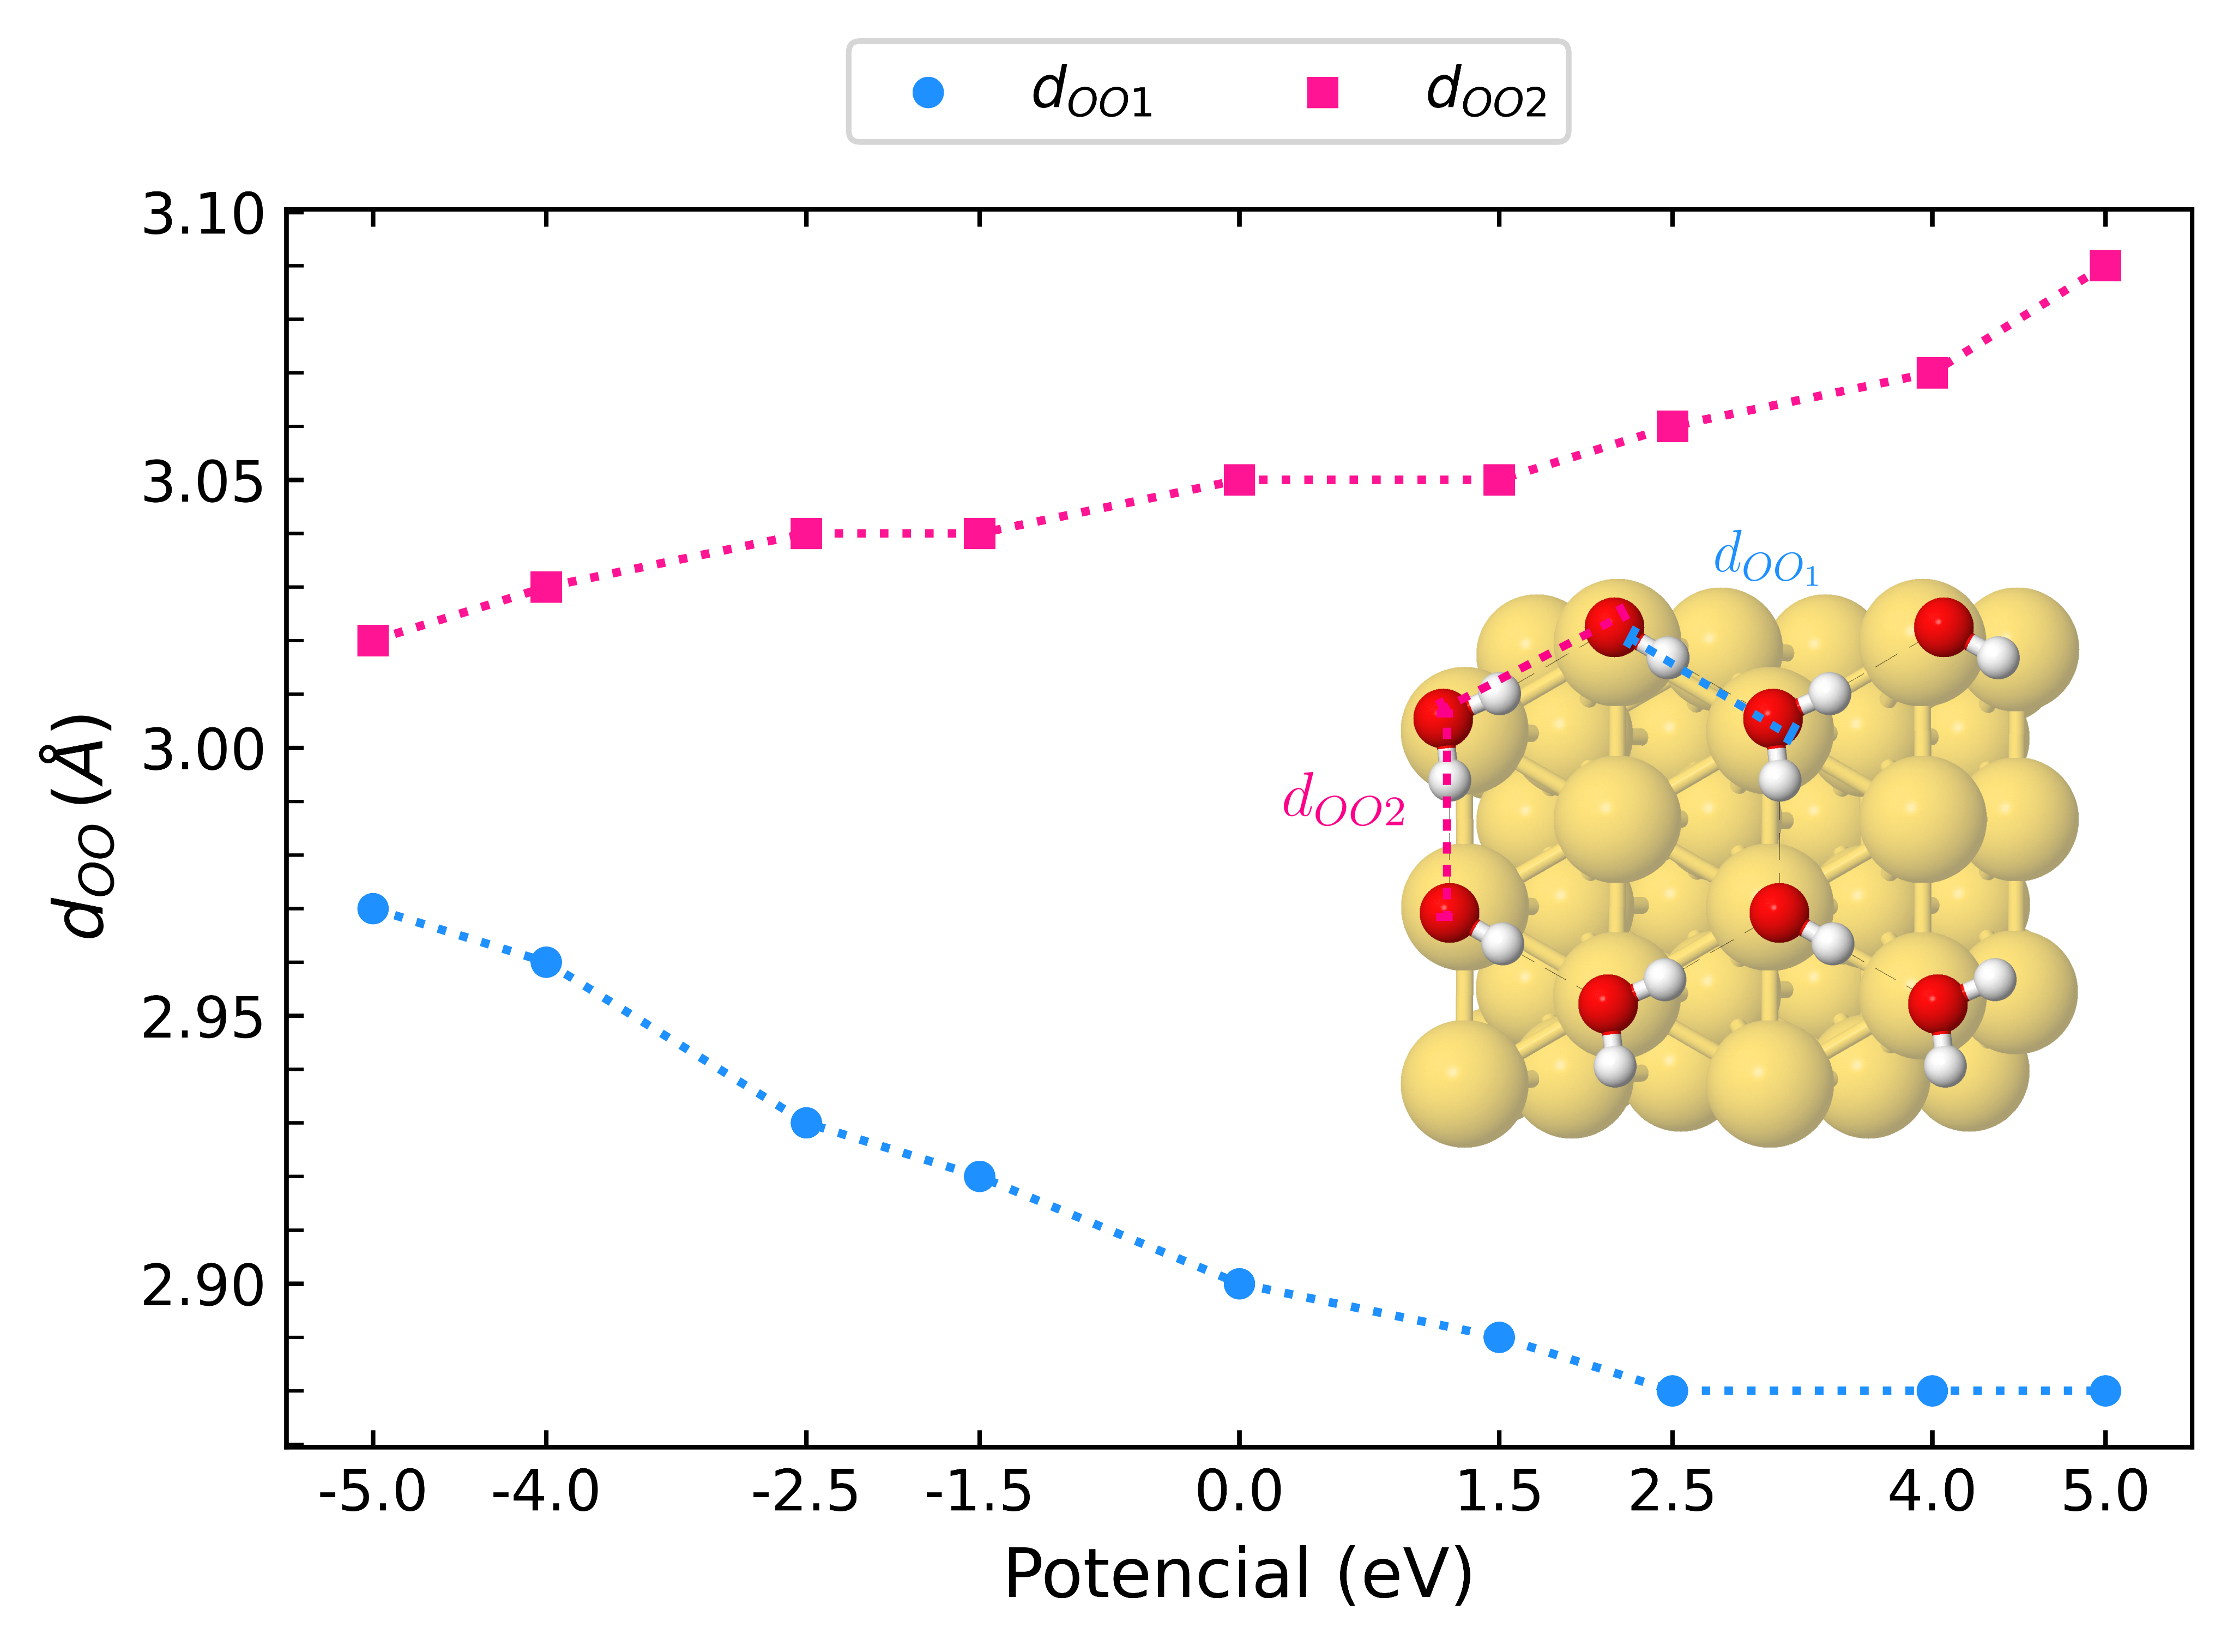
\includegraphics[width=\textwidth]{figs/distancia_oo.png}
		\legend{Fonte: compilação da autora.}
		\label{fig:distancia_oo}
	\end{subfigure}
\end{figure}

Dessa forma, a camada de água estudada nesse trabalho possuía 8 moléculas dispostas num arranjo hexagonal semelhante ao do gelo (\textit{ice bilayer Ih}) em uma célula de tamanho $ (\sqrt{3}\times\sqrt{3})R30 $ em relação ao parâmetro estrutural do Au ($ 4.24\,\si{\angstrom} $). Os eletrodos metálicos eram compostos por 3 camadas com o plano metálico formado por $ 3\times 4$ átomos nas direções $ xy $. O tamanho da célula unitária utilizada foi $ 10.40\times9.00\times 54.21\,\si{\angstrom} $. O funcional de troca e correlação utilizado foi o PBE e as relaxações foram realizadas com os potencias externo variando entre -5.0 a 5.0 eV, com intervalos entre 1.0 a 1.5 eV. Após obter as coordenadas minimizadas, obteve-se as frequências de vibrações do sistema.

Em relação às moléculas na orientação \textit{flat-down}, observa-se variações máximas de $\Delta_{d,máx}= 0.09\,\si{\angstrom} $ e da inclinação $\Delta_{\alpha,máx}= 3\si{\degree} $, ao passo que as variações máximas das moléculas \textit{flat} foram $\Delta_{d,máx}= 0.57\,\si{\angstrom} $ e $\Delta_{\alpha,máx}= 25\si{\degree} $, respectivamente (Tabela \ref{tab:neq_au_geo}). Para potenciais positivos, as moléculas tendem a se afastar da superfície metálica, enquanto que para potenciais negativos as moléculas se aproximam do metal. Além disso, é possível ver o efeito da competição entre a interação água/metal e a ligação de hidrogênio, uma vez que, as variações das distâncias e das inclinações são menores que as observadas no monômero. Esse efeito também é visto pelo aumento da ligação $ d_{O-H} $ em relação ao monômero $ d_{O-H}\sim0.97\,\si{\angstrom} $; para as moléculas \textit{flat-down} a distância $ d_{O-H} $ da ligação O-H que interage com o metal foi $ 0.98\,\si{\angstrom}  $, ao passo que a ligação O-H que participa da ligação de hidrogênio foi $ 0.99\,\si{\angstrom}  $. Esses valores são inferiores aos observados na camada de água \textit{H-Down} adsorvida no Pd(111), onde obtivemos $ d_{OH}=0.99\,\si{\angstrom} $ para a ligação O-H que participa da ligação de hidrogênio e $ d_{OH}=1.00\,\si{\angstrom} $ para a ligação que interage com o metal. Esse resultado revela o efeito das propriedades reativas do metal sobre a adsorção de estruturas de água.

O efeito do potencial externo afeta principalmente as moléculas \textit{flat}, uma vez que as propriedades geométricas das moléculas \textit{flat-down} apresentaram alterações pequenas com a variação do potencial. Ademais, observa-se que os ângulos $ \Theta $ das moléculas \textit{flat} são maiores do que os da molécula \textit{flat-down}. Além disso, é possível ver o comportamento assimétrico das propriedades geométricas em relação ao sinal do potencial aplicado. Isso é visto através da inclinação $ \alpha $ que somente troca de sinal a partir de V=2.5 eV, diferentemente do caso do monômero. Além disso, observa-se que as moléculas se afastam do metal e diminuem a inclinação para potenciais positivos e se aproximam e aumentam a inclinação para V<0. Esses processos ocorrem de forma quase linear e refletem atração/repulsão resultante da polarização superficial e o aumento/diminuição da repulsão de Pauli.

\begin{figure}[t!]
	\centering
	\caption{(a) Diferenças de densidades de carga $ \Delta \rho_{V} $ da camada de água adsorvida no Au(111) para os potenciais 1.5 e 5.0 eV. Os valores de isosuperfícies dos gráficos de $ \Delta\rho_{+V} $ e $ \Delta\rho_{-V} $ correspondem a $ 3.97\times10^{-4}\;\si{e}/\si{\angstrom}^3 $. Na última coluna estão representados as flutuações de densidades de carga com os respectivos valores de isosuperfícies $ 3.35\times10^{-5}$ e $ 1.60\times10^{-5}$. Em todos os casos, azul (vermelho) indica uma deficiência (excesso) de elétrons. (b) Gráfico das diferenças de densidades de carga média ao longo do eixo z para os potenciais $ V=\pm1.5\,\pm2.5$ e $ \pm5.0\,\si{\eV} $. No gráfico também estão representados as posições da última camada de Au, dos átomos de H das moléculas \textit{flat-down} que interagem com o metal e dos átomos de oxigênio das moléculas \textit{flat-down}.}
	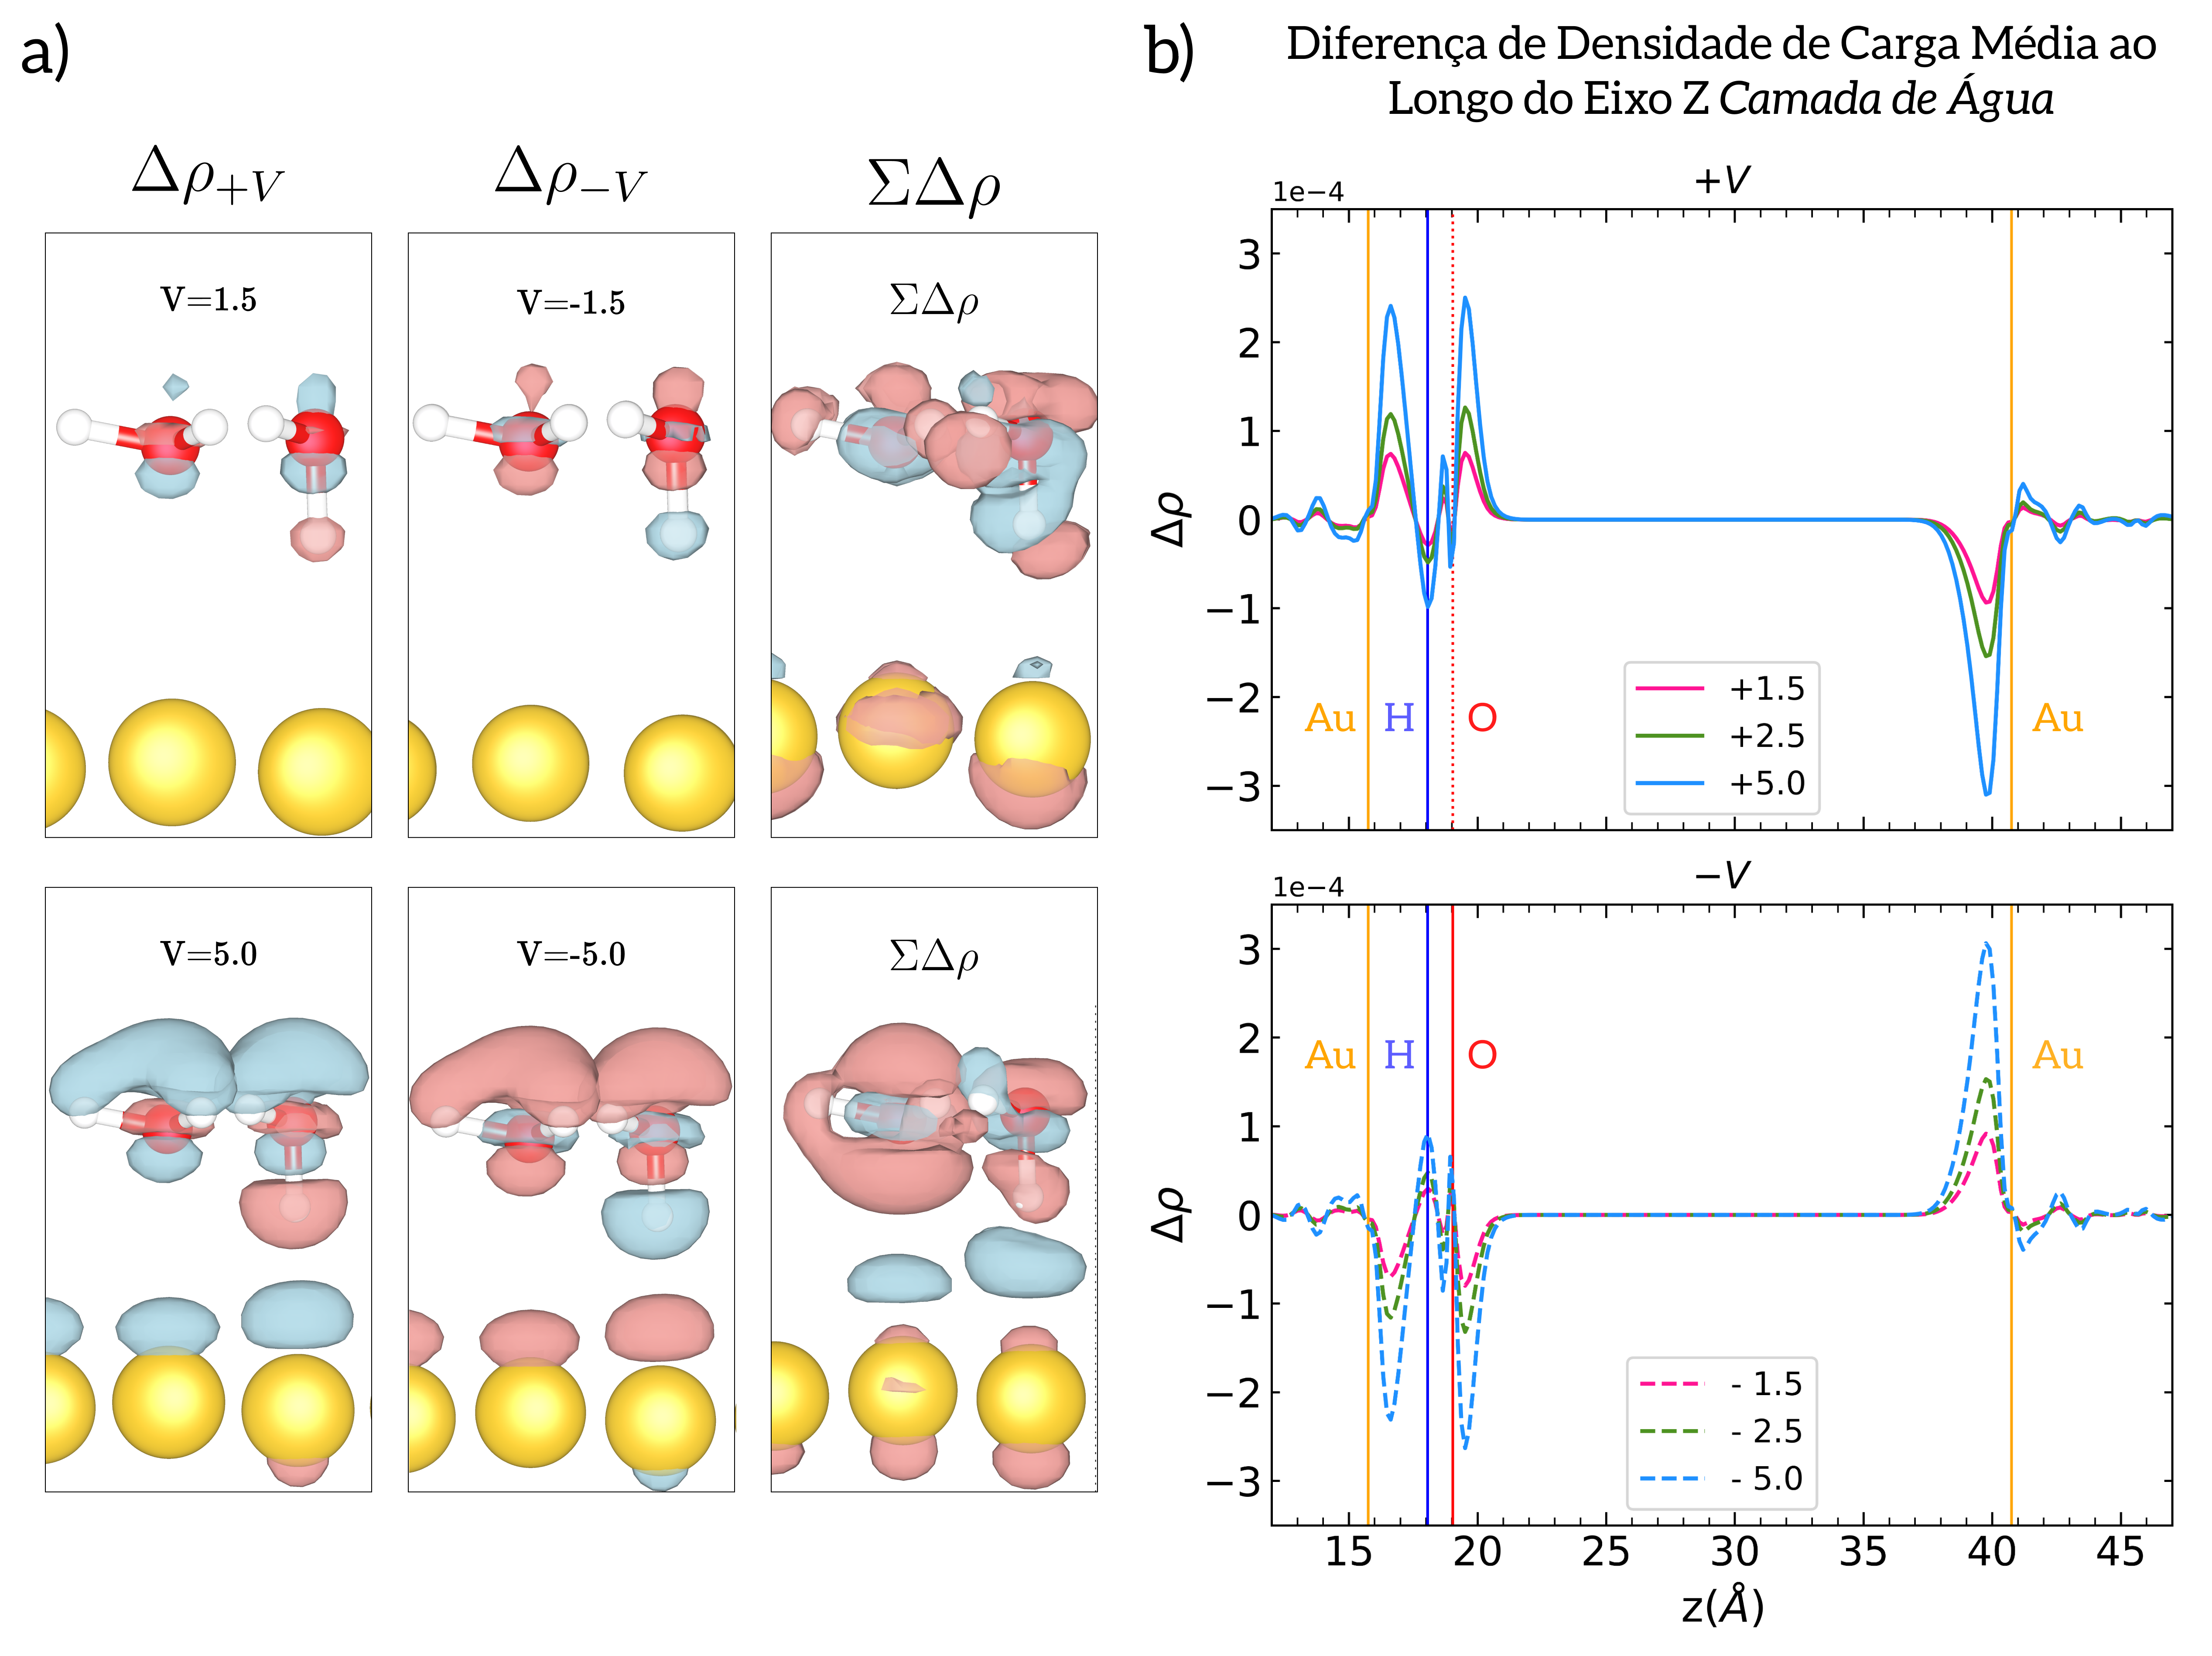
\includegraphics[scale=0.075]{figs/au_densidade_layer.png}
	\legend{Fonte: compilação da autora.}
	\label{fig:neq_au_dens}
\end{figure}

Dentre as propriedades geométricas, analisamos também as distâncias entre os átomos de oxigênio $ d_{OO1} $ e $ d_{OO2} $, no qual $ d_{OO1} $ refere-se às distâncias onde as moléculas \textit{flat-down} atuam como doadoras e $ d_{OO2} $ considera as distâncias onde as moléculas \textit{flat} que agem como doadoras (Figura \ref{fig:distancia_oo}). Assim, observa-se que para potenciais negativos têm-se uma maior variação das distâncias $ \Delta d_{OO1}=0.07\,\si{\angstrom} $. Para potenciais positivos essa distância se mantém praticamente constante, enquanto que $ d_{OO2} $ aumenta em até $ 0.04\,\si{\angstrom} $.


Para melhor compreender o efeito do potencial sobre as interações obtivemos os gráficos de diferença de densidade de carga e a média ao longo do eixo z -- Figura \ref{fig:neq_au_dens}. Através do gráfico de $ \Delta\rho_{_ {V}} $, observa-se que a concentração de densidade de carga está no átomo de O e que as variações de densidade e as transferências de carga são proporcionais ao potencial aplicado. Isso resulta na atração das moléculas \textit{flat} e \textit{flat-down} em direção à superfície metálica para V<0 e no comportamento contrário para V>0. Além disso, através da densidade média ao longo do eixo z, Figura \ref{fig:neq_au_dens} (b), observa-se que a transferência de carga entre as moléculas e o metal ocorre através da molécula \textit{flat-down} é maior. Isso é visto através da variação de carga que ocorre na posição correspondente ao átomo de hidrogênio próximo ao metal. %Através desses gráficos é possível também visualizar a interação entre as moléculas de água.% Por fim, observa-se .

Por fim, analisamos o efeito do potencial sobre as frequências dos modos normais de vibrações. Como o sistema é composto por 8 moléculas, então exitem 18 frequências fundamentais que foram representadas por uma distribuição normalizada (Figura \ref{fig:neq_au_freq}). Além disso, os valores superiores e inferiores das vibrações das frequências de \textit{bending} e \textit{stretching} estão representadas na Tabela \ref{tab:neq_freq_camada}. Através da projeção da densidade total de estados sobre as frequências vibracionais foi possível associar os picos às interações dominantes (interação água/água ou água/metal) e ao tipo de vibração (\textit{stretching simétrico ou assimétrico}). Assim, os valores representados na Figura \ref{fig:neq_picos} correspondem às frequências dos picos dominantes de acordo com a orientação da molécula responsável pela vibração dominante.

De modo geral, observa-se que as frequências inferiores estão associadas às vibrações de \textit{stretching} simétrica das moléculas \textit{flat-down} e correspondem à ligação O-H que participa da ligação de hidrogênio. Logo, essas ligações representam ligações O-H mais fracas, como pode ser visto pelo aumento da distância $ d_{OH} $, e ligações de hidrogênio mais intensas. As frequências intermediárias correspondem às vibrações de \textit{stretching} simétrica das moléculas \textit{flat} e de \textit{stretching} assimétrica das moléculas \textit{flat-down}. Essas últimas estão associadas às ligações O-H que interagem com o metal. As frequências maiores representam as vibrações de \textit{stretching} assimétrico das moléculas \textit{flat}. Além disso, observa-se que todas as frequências estão abaixo das frequências de \textit{stretching} assimétricos do dímero isolado.

Conforme o potencial aumenta negativamente, as frequências de \textit{stretching} tendem a se agrupar (Figura \ref{fig:neq_au_geo_layer}), de forma que os valores de \textit{stretching} inferiores aumentam e superiores diminuem -- Tabela \ref{tab:neq_freq_camada}. Além disso, observa-se pela Figura $\ref{fig:neq_picos}$ que as frequências das moléculas \textit{flat} tendem a diminuir, enquanto que as moléculas \textit{flat-down} aumentam. Esse resultado associado ao aumento da distância $ d_{OO1} $ da molécula \textit{flat-down} que atua na ligação de hidrogênio como doadora representa ligações de hidrogênio mais intensas e interações água/metal mais fracas. % Esse resultado condiz com observações experimentais nos quais mostram que a densidade superficial de água aumenta quando o metal está carregado positivamente e as frequências diminuem \cite{kramer} \cite{bibid}


Para potenciais positivos, observa-se uma dispersão das frequências, de forma que as frequências de \textit{stretching} superiores aumentam e as inferiores diminuem (Tabela \ref{tab:neq_freq_camada}). Além disso, observa-se um aumento das frequências assimétricas das molécula \textit{flat} e \textit{flat-down}, sendo mais proeminente para as frequências das moléculas \textit{flat-down}. Essas últimas estão relacionadas à interação água/metal e representa um enfraquecimento da interação água/metal. Ademais, o aumento nas frequência da molécula \textit{flat} refletem o crescimento da distância $ d_{OO2} $, de forma que as ligações de hidrogênio também são afetadas. 

%O modelo aqui analisado considerou o efeito do potencial externo sobre interações tipo água/água e água/metal. Através das propriedades analisadas, observa-se que  
\begin{figure}[b!]
	\centering
	\caption{Gráfico das frequências de \textit{stretching} características das interações dominantes de acordo com o potencial externo aplicado. As frequências foram separadas de acordo com a orientação da molécula (\textit{flat} e \textit{flat-down}) e pelo tipo de vibração (simétrico(S) e assimétrico(AS)). }
	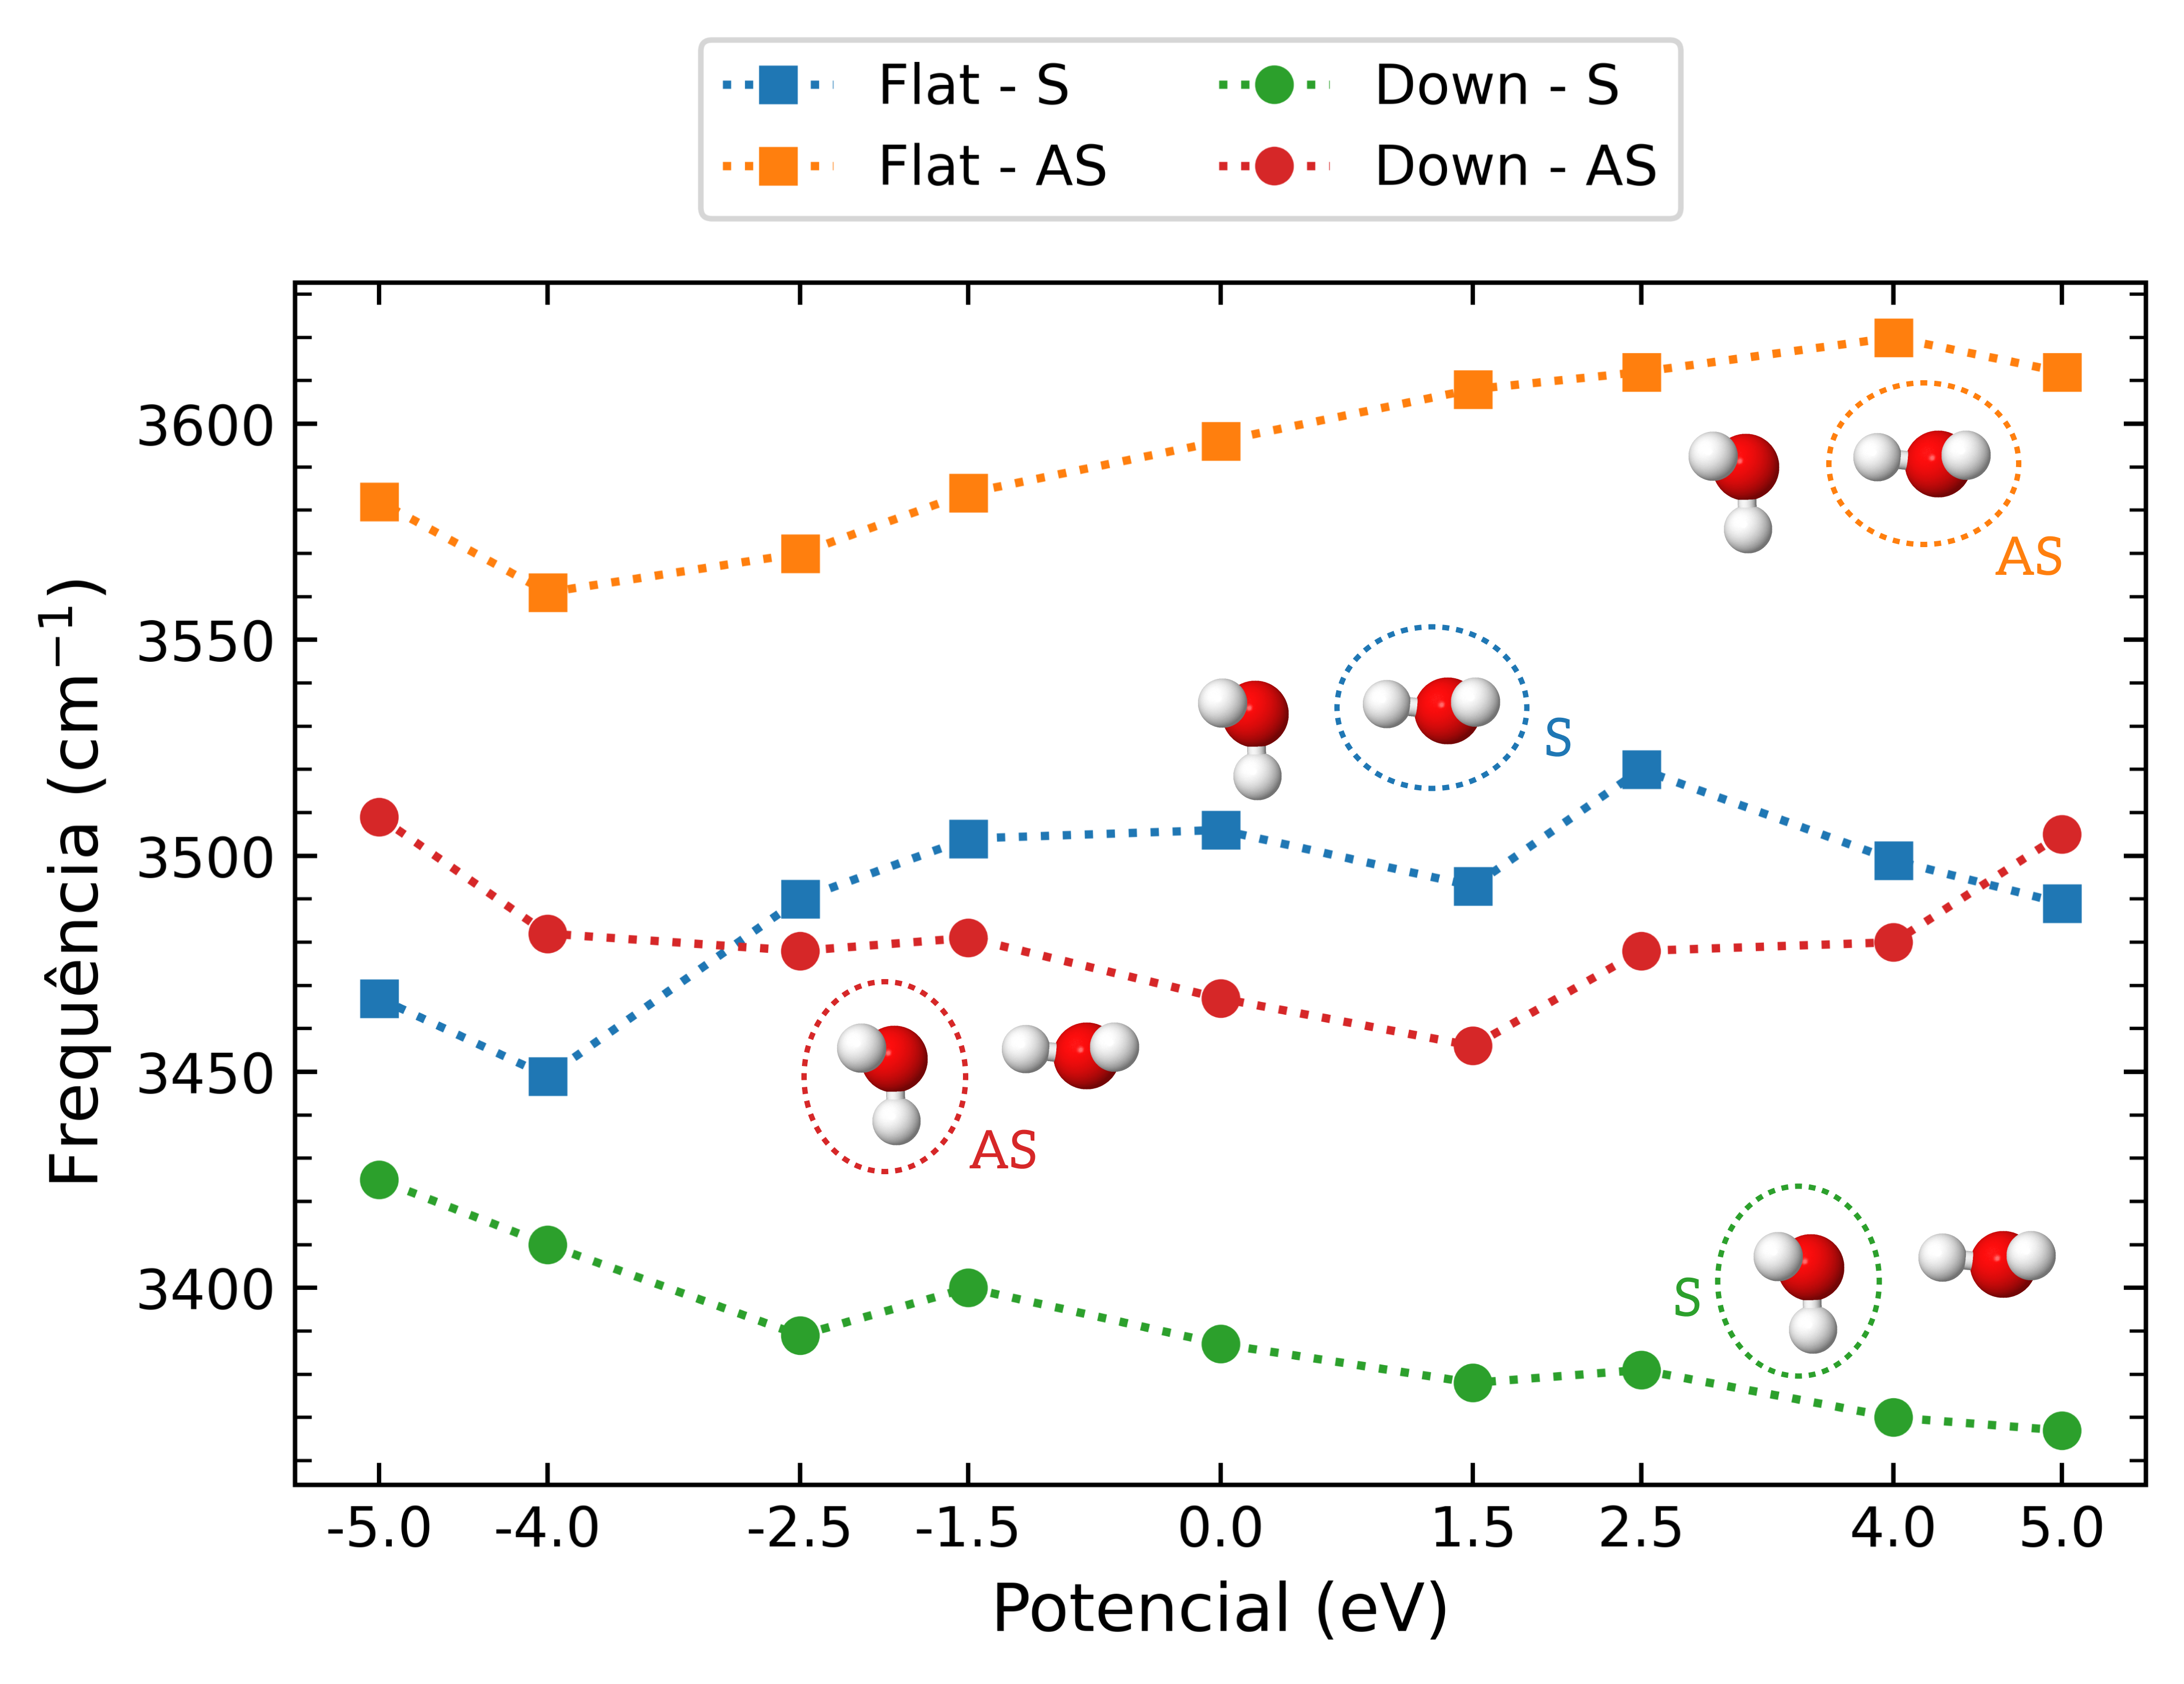
\includegraphics[scale=0.085]{figs/layer_picos.png}
	\legend{Fonte: compilação da autora.}
	\label{fig:neq_picos}
\end{figure}
Apesar do modelo estudado fornecer detalhes sobre  o efeito do potencial externo sobre interações tipo água/água e água/metal de uma camada de água, esse modelo não inclui interações das moléculas de água com a água \textit{bulk} ou o efeito do potencial sobre moléculas não-ligadas. Em particular, a presença da água \textit{bulk} é fundamental para compreender processos de oxidação e redução na superfície metálica carregada e têm sido investigada através da implementação de modelos contínuos \cite{bias_agua1,review_new}.  

Dessa forma, os resultados aqui encontrados mostraram que o potencial externo afeta principalmente as ligações de hidrogênio. Isso é visto pelas mudanças provocadas nas propriedades geométricas e vibracionais das moléculas \textit{flat}, uma vez que essas moléculas se aproximam do metal para potenciais negativos e se distanciam para potenciais positivos. Além disso, potenciais negativos intensificaram as ligações de hidrogênio, ao passo que potenciais positivos enfraqueceram tanto as ligações de hidrogênio quanto as interações água/metal. Por outro lado, através dos gráficos de $ \Delta\rho_{V} $ observa-se um excessos/deficiência de elétrons na região entre as moléculas \textit{flat-down} e o metal. Isso mostra que essas moléculas estão mais ligadas ao metal e portanto são menos afetadas pelo efeito do potencial externo.

 
\begin{table}[H]
	\centering
	\caption{Tabela contendo as principais frequências de vibração da camada adsorvida de acordo com cada funcional, bem como as frequências experimentais e teóricas do dímero isolado. \label{tab:neq_freq_camada}}
	\begin{threeparttable}
		\begin{tabular}{Scccccc} 
			\hline\hline
			\multicolumn{7}{c}{ \textbf{Frequências dos Modos Normais (\si{\cm}$ ^{-1} $) - Camada de Água} }                                                                                                                                                 \\ 
			\midrule
			{\multirow{2}{*}{V (eV)}}                                                  &  & \multicolumn{2}{c}{\textit{Bending }} &  & \multicolumn{2}{c}{\textit{Stretching}}                                                                            \\ 
			\cmidrule{3-4}\cmidrule{6-7}
			&  & Inferior & Superior                   &  & Inferior                                                 & Superior                                                \\ 
			\midrule
			-5.0                                                                     &  & 1616     & 1671                       &  & 3416                                                     & 3582                                                    \\
			-4.0                                                                     &  & 1621     & 1668                       &  & 3401                                                     & 3561                                                    \\
			-2.5                                                                     &  & 1622     & 1670                       &  & 3386                                                     & 3570                                                    \\
			-1.5                                                                     &  & 1623     & 1673                       &  & 3389                                                     & 3584                                                    \\
			0.0                                                                      &  & 1624     & 1672                       &  & 3369                                                     & 3596                                                    \\
			1.5                                                                      &  & 1625     & 1669                       &  & 3365                                                     & 3608                                                    \\
			2.5                                                                      &  & 1629     & 1668                       &  & 3365                                                     & 3612                                                    \\
			4.0                                                                      &  & 1633     & 1659                       &  & 3364                                                     & 3620                                                    \\
			5.0                                                                      &  & 1639     & 1656                       &  & 3353                                                     & 3612                                                    \\ 
			\midrule
			{Dímero Isolado~Exp.\tnote{$\dagger$}}&  & \multicolumn{2}{c}{1618.1}            &  & \begin{tabular}[c]{@{}c@{}}3547.5\\ 3697.7 \end{tabular} & \begin{tabular}[c]{@{}c@{}}3625.5\\3714.7\end{tabular}  \\
			\hline\hline
		\end{tabular}
		\begin{tablenotes}\footnotesize
			\item[$\dagger$]\citeauthor{ref-modos}
		\end{tablenotes}
	\end{threeparttable}
\end{table}





\begin{figure}[H]
	\centering
	\caption{Distribuição das frequências de vibrações ($\si{\cm}^{-1}$) das camadas de acordo com o potencial aplicado ($ \si{\eV} $). Os marcadores verticais representam os valores discretos das frequências. Além disso, está representado a interação dominante e a respectiva frequência; a linha tracejada representa as frequências experimentais do dímero isolado.}
	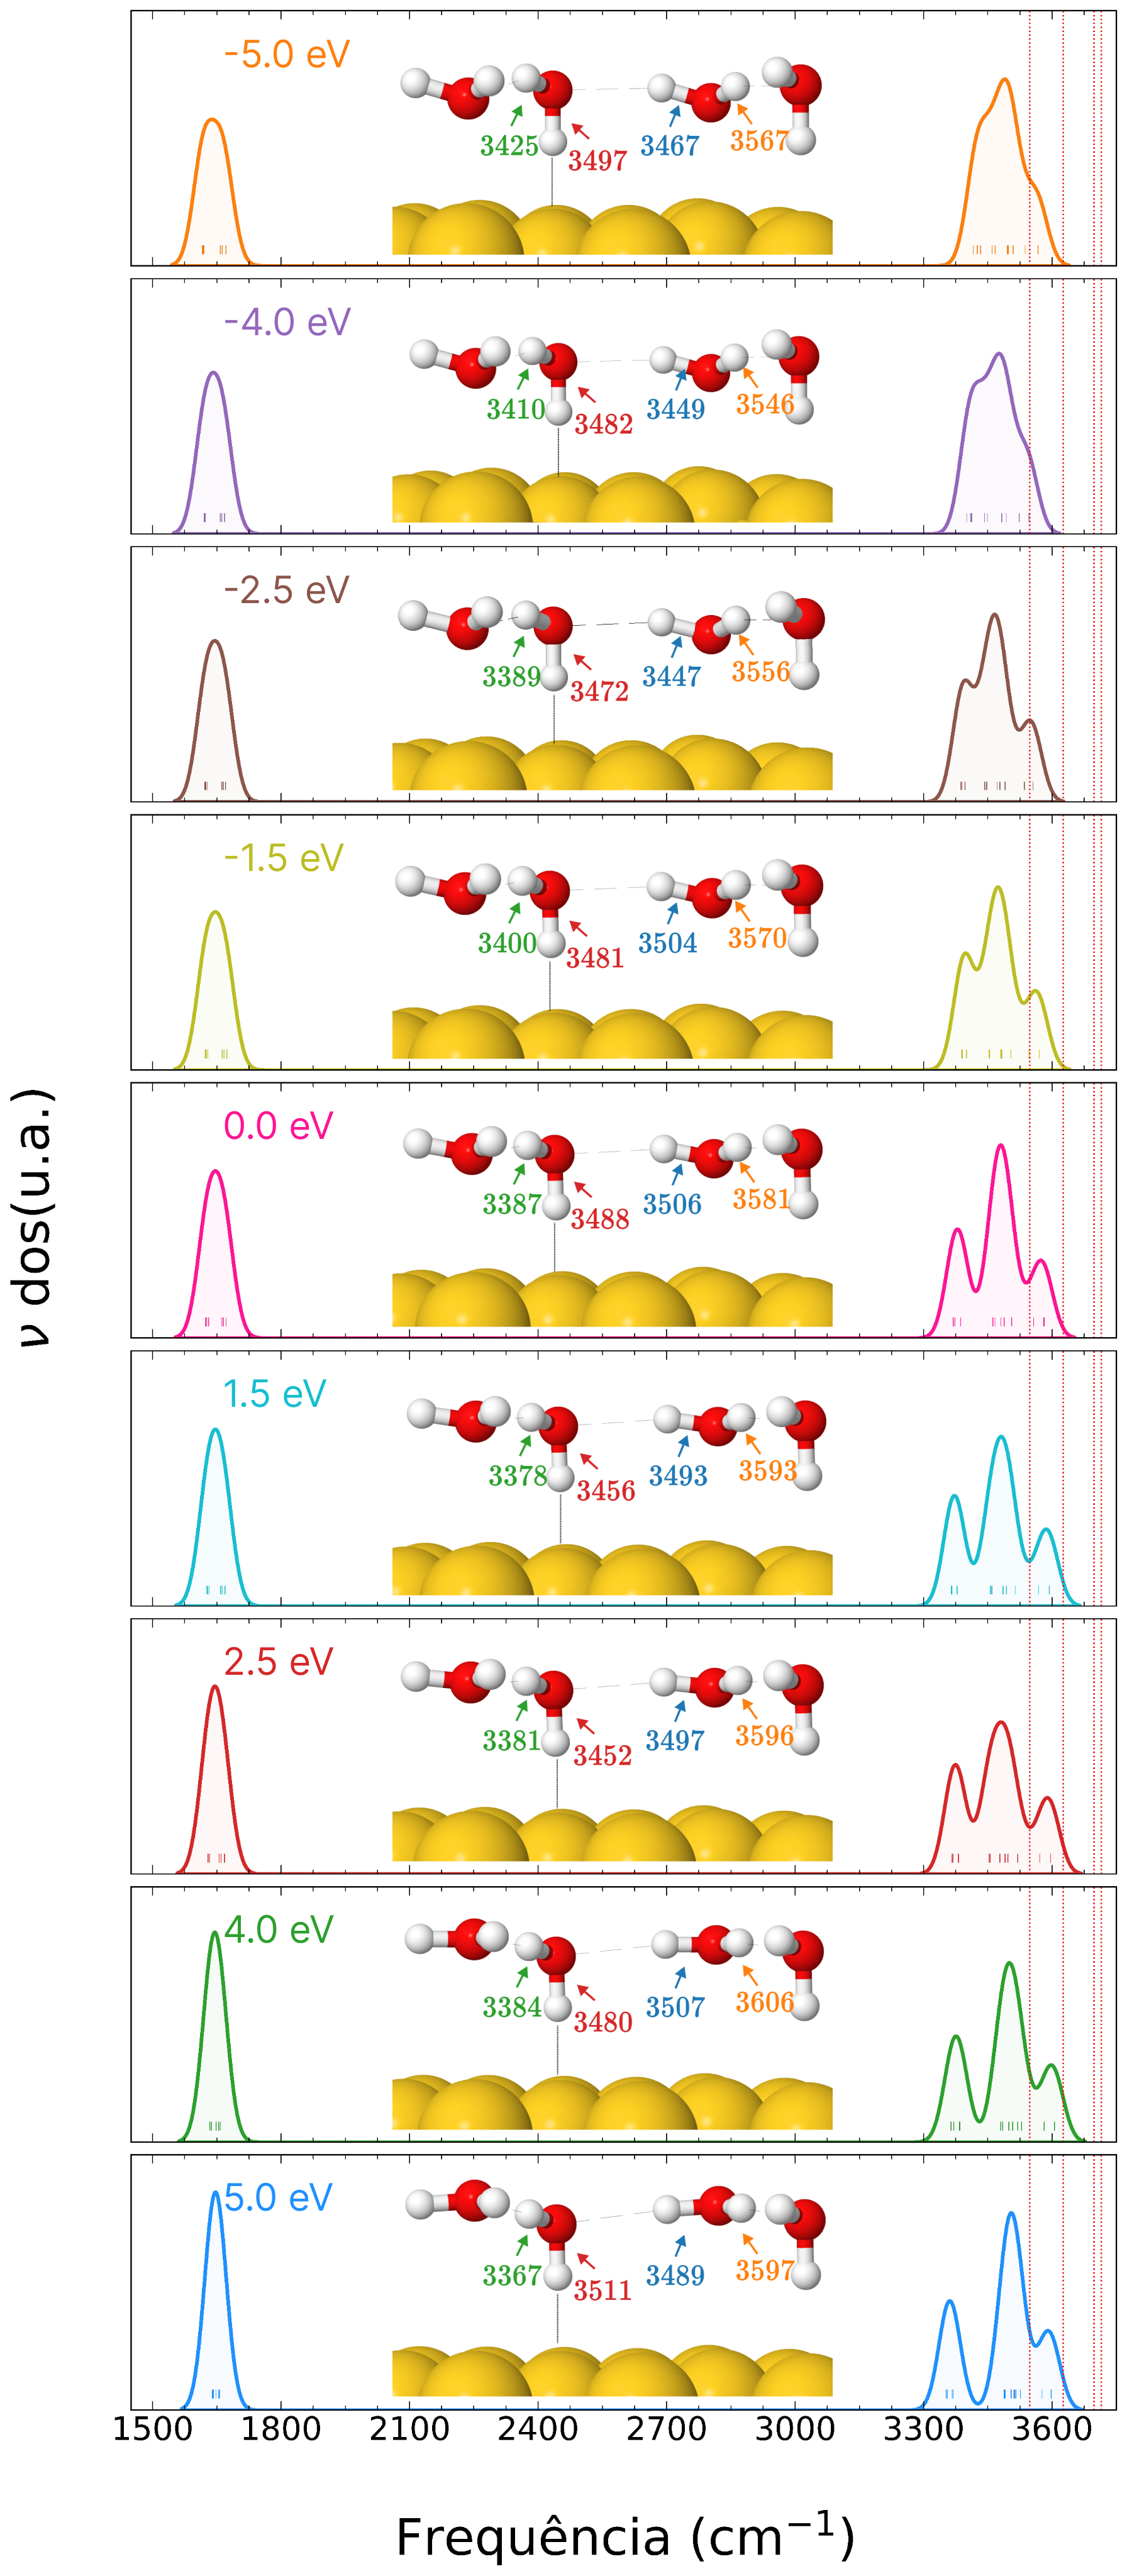
\includegraphics[scale=0.15]{figs/freq_layer.jpg}
	\legend{Fonte: compilação da autora.}
	\label{fig:neq_au_freq}
\end{figure}


% ---

% Finaliza a parte no bookmark do PDF, para que se inicie o bookmark na raiz
% ---
\bookmarksetup{startatroot}% 
% ---

% ---
% Conclusão
% ---
% ---
% Capitulos:
% ---

\chapter[Conclusões]{Conclusões \label{cap:conclusao}}
%\addcontentsline{toc}{chapter}{Conclusão}

Nesse trabalho realizamos a descrição atomística da interface água/metal sem a presença de perturbações externas e considerando a aplicação de um potencial externo. Isso foi feito através da adsorção de um monômero e uma camada de água em superfícies metálicas. Para aplicar a diferença de potencial foi utilizado formalismo de NEGF+DFT e o efeito do potencial externo foi mensurado através das propriedades estruturais, eletrônicas e vibracionais. 

Primeiramente, caracterizamos a interface água/metal sem a presença de perturbações externas. A partir da análise do monômero adsorvido no Pd(111), encontramos que a orientação mais estável é a orientação \textit{flat}, seguida da orientação \textit{up}. Além disso, obtivemos que as forças de dispersão de van der Waals são relevantes na descrição das interações água/metal e afetam as energias de adsorção e as propriedades vibracionais. A acurácia e precisão desses resultados foram fundamentadas pelos testes de convergência de pontos \textit{k} e tamanho de superfície.

Em seguida, aumentamos a complexidade do sistema e realizamos simulações com três tipos de camadas bidimensionais: H-Down, H-Up e H-Down/Up. Assim, foi possível caracterizar a competição entre as ligações de hidrogênio e interações água/metal. Essa caracterização mostrou que a camada H-Down é a mais estável devido à presença das interações entre as moléculas de água \textit{flat-down} e o metal.

Após descrever a interface água/Pd(111) sem a presença de perturbações externas, analisamos como a aplicação do potencial externo afeta o comportamento dessa interface e também do monômero adsorvido no Au(111). De modo geral, observamos que para potenciais positivos a molécula tende a se afastar do eletrodo metálico, ao passo que para potenciais negativos a molécula tende a se aproximar da superfície carregada. Como resultado, as frequências de \textit{stretching} diminuem para potenciais positivos e vice-versa. Assim, a posição de mínima energia do monômero é resultado do efeito eletrostático somado ao efeito do potencial sobre a repulsão de Pauli. 

Além disso, observamos que a reatividade do metal afeta fortemente o comportamento da molécula de água na superfície carregada. Para tanto, observamos que para um mesmo valor de potencial, as distâncias $ d_{OM} $ e a inclinação $ \alpha $ do monômero adsorvido no Au(111) foram superiores às do Pd(111). Consequentemente, as frequências vibracionais do Pd(111) foram menores. Além disso, observamos que o potencial externo afetou o sítio preferencial de adsorção do monômero nos dois metais.

Uma vez caracterizado o efeito do potencial externo sobre a interação água/metal, investigamos como o potencial afeta ligações de hidrogênio. Para isso, utilizamos a camada H-Down adsorvida no Au(111) e observamos que o potencial externo afera principalmente o comportamento estrutural das moléculas \textit{flat}. Assim, as moléculas \textit{flat} reproduzem o comportamento observado no monômero mas com menor intensidade.


Em relação às propriedades vibracionais, observa-se que as frequências inferiores descrevem as ligações O-H das moléculas \textit{flat-down} que participam das ligações de hidrogênio e as frequências superiores correspondem às ligações O-H das moléculas \textit{flat}. Além disso, observamos que potenciais negativos intensificam as ligações de hidrogênio e potenciais positivos enfraquecem as interações água/metal e ligações de hidrogênio.

Através do cálculo de forças fora do equilíbrio, conseguimos realizar a otimização das coordenadas dos sistemas água/metal e obter as propriedades estruturais, eletrônicas e vibracionais. Assim, como perspetiva futura é importante analisar o comportamento das estruturas ao aplicar potenciais maiores, bem como analisar o efeito do potencial sobre estruturas maiores de água. Além disso, como esse formalismo permite o cálculos de forças fora do equilíbrio, é possível, em princípio, estender esse formalismo a simulações de dinâmica molecular \textit{ab initio}, bem como incluir o efeito de solventes através de modelos contínuos.

% ----------------------------------------------------------
% ELEMENTOS PÓS-TEXTUAIS
% ----------------------------------------------------------
\postextual


% ----------------------------------------------------------
% Referências bibliográficas
% ----------------------------------------------

\bibliography{monografia.bib}

%\printbibliography
% ----------------------------------------------------------
% Glossário
% ----------------------------------------------------------
%
% Consulte o manual da classe abntex2 para orientações sobre o glossário.
%
%\glossary

% ----------------------------------------------------------
% Apêndices
% ----------------------------------------------------------

% ---
% Inicia os apêndices
% ---
\begin{apendicesenv}

% Imprime uma página indicando o início dos apêndices
\partapendices
\chapter{Teoria do Funcional da Densidade \label{provas}}

\section{Postulados da Mecânica Quântica\label{meq}}

Ao estudar as propriedades de átomos, moléculas e sólidos é fundamental obter as autofunções da Hamiltoniana que descreve o sistema:
\begin{equation}
	\hat{H}=\hat{T}+\hat{V}
\end{equation}

Nesses sistemas, a contribuição para o potencial é devido às interações entre núcleo-núcleo, núcleo-elétron e elétron-elétron. A interação núcleo-elétron é uma interação Coulombiana entre o núcleo e cada elétron, onde considera-se os elétrons sujeitos a um potencial externo, o potencial do núcleo; a interação elétron-elétron ocorre entre um par de elétrons.

O termo de energia cinética é dado pela soma das energias cinéticas dos elétrons e do núcleo. Por outro lado, como a massa do núcleo é significativamente maior que a massa do elétron, a contribuição do núcleo pode ser separada da parte eletrônica. Essa é a chamada  \textit{Aproximação de Born-Oppenheimer} \cite{material_1}.

Logo, a hamiltoniana de um sistema de $ N_e $ elétrons e $ N_n $ núcleos é dada pela expressão:
\begin{eqnarray}\label{eq:ham_complete}
	\hat{H} &=& \hat{T}_{e}+\hat{V}_{ne}+\hat{V}_{ee}+\hat{V}_{nn}  \\
	&=& -\frac{\hbar^2}{2m_e}\sum_{i}^{N_e} \grad^2_i+\frac{e^2}{4\pi \epsilon_0}\bqty{-\sum_{i}^{N_e}\sum_{I}^{N_n} \frac{Z_I}{\abs{\vb{r}_i-\vb{R}_I}} +\frac{1}{2}\sum_{i}^{N_e}\sum_{j\neq i}^{N_e}\frac{1}{\abs{ \vb{r}_i-\vb{r}_j}} +\frac{1}{2}\sum_{I}^{N_n}\sum_{J\neq I}^{N_n}\frac{Z_I Z_J}{\abs{\vb{R_I}-\vb{R_J}}}}  \nonumber
\end{eqnarray}

Onde para posições $ \vb{R_I}$ e $ \vb{R_J} $ mantidas fixas, são feitos os cálculos para a parte eletrônica.

Para descrever o estado físico e a evolução temporal de uma função de onda de N elétrons é necessário recorrer aos postulados da Mecânica Quântica, dentre os quais vale destacar três:

\begin{enumerate}
	\item O \textit{estado físico} de um sistema de N elétrons sujeito a um potencial externo é representado por uma \textit{Função de Onda} $\Psi(\vb{x_1},\vb{x_2},\ldots,\vb{x_N},t)$, onde $ \vb{x}=(\vb{r},\xi)$ representa a coordenada espacial e a coordenada de spin. Essa função de onda contém toda a informação do sistema.
	\item A evolução temporal da \textit{Função de Onda} de um sistema obedece à Equação de Schr\"{o}dinger dependente do tempo:
	\begin{equation}\label{eq:schr}
		i\hbar \pdv{\Psi}{t} = \hat{H}\Psi
	\end{equation} 
	\textbf{Observação:} Quando o potencial não depende do tempo, $ \Psi $ pode ser escrito como o produto de uma função dependente do tempo e por outra que dependa apenas de $ \vb{r} $. A parte dependente da posição satisfaz à Equação de Schr$ \"{o} $dinger  independente do tempo:
	\begin{equation}
		\hat{H}\Psi=E\Psi
	\end{equation}
	\item \label{post_anti} A função de onda de um sistema composto por N partículas idênticas pode ser \textit{simétrica} ou \textit{antissimétrica} de acordo com a permutação de um par de partículas.
	\begin{equation}
		\Psi(\vb{x_1},\ldots,\vb{x_i},\vb{x_j},\ldots,\vb{x_N})=\pm \Psi(\vb{x_1},\ldots,\vb{x_j},\vb{x_i},\ldots,\vb{x_N})
	\end{equation}
	
	As partículas com spin inteiro possuem estados simétricos e são denominadas \textit{bósons} e partículas com spin semi-inteiro possuem estados antissimétricos e são chamados de \textit{férmions}. \cite{Zettili}
	
\end{enumerate} 
Considerando o elétron, cujo spin é $ s=\frac{1}{2} $, a função de onda de uma partícula ou orbital, pode ser escrita pela expressão abaixo, onde $R_{n,l}$ é a solução da parte radial com os números quânticos \textit{n} e \textit{l}; $ \mathrm{Y}_{l,m_l}(\theta,\varphi) $ é a parte angular, cuja solução corresponde aos harmônicos esféricos com os números quânticos \textit{l} e $ m_l $ e $ \chi(\xi) $ é a solução da parte de spin, no qual os números quânticos correspondentes são $s=\frac{1}{2}$ e $ m_s=\pm \frac{1}{2} $.
\begin{equation}
	\varphi_{n,l,m_l,m_s}(\vb{r},\xi)=R_{n,l}(r)\mathrm{Y}_{l,m_l}(\theta,\phi)\chi_{\frac{1}{2},m_s}(\xi)
\end{equation}

De acordo com o Postulado descrito no item \ref{post_anti}, a função de N-partículas de um sistema sujeito à interação coulombiana deverá ser anti-simétrica, por se tratar de férmions. Tal função é descrita em termos do operador \textit{Permutação} ($ \hat{P} $), cuja ação realiza a permutação entre duas coordenadas $ \vb{x_i} $ e $ \vb{x_j} $. O resultado dessas permutações é denominado \textit{Determinante de Slater}.
\begin{equation}\label{eq:wave_anti}
	\Psi(\vb{x_1},\vb{x_2},\ldots,\vb{x_N})=\frac{1}{\sqrt{N!}}\sum^{N!}_{i=1}(-1)^{P}\hat{P}\bqty{\varphi_{n_{1},l_{1},m_{l_{1}},m_{s_{1}}}(\vb{x_1}),\ldots,\varphi_{n_{N},l_{N},m_{l_{N}},m_{s_{N}}}(\vb{x_N})}
\end{equation}

A solução exata da equação \eqref{eq:schr}, cuja hamiltoniana corresponde à equação \ref{eq:ham_complete} é inviável de ser obtida analiticamente, de modo que é necessário métodos sofisticados de aproximação teórica e computacional. Em resumo, existem duas grandes divisões nos métodos de aproximação: aproximações \textit{baseadas na função de onda}, onde \textit{Hartree-Fock} é um exemplo desse tipo, ou aproximações \textit{baseadas na densidade eletrônica}, tal como a \textit{Teoria do Funcional da Densidade (DFT)}. \cite{hf_pedroza}

\section{Teoremas de Hohenberg-Kohn}

\begin{lema}
	O valor esperado do operador que representa o potencial externo $ \hat{W} $ é dado por:
	\begin{equation}
		\ev{\hat{W}}{\Psi}= \int w(\vb{r})\dens\dr
	\end{equation} 
\end{lema}

\begin{proof}
	Em um sistema de N elétrons, cuja função de onda é dada por $ \Psi= \Psi(\vb{r}_1,\ldots,\vb{r}_N) $, onde a parte de spin é ignorada, o valor esperado do operador Potencial Externo é dado por:
	\begin{equation}
		\ev{\hat{W}}{\Psi}=-\sum_{i}^{N} \sum_{I}^{N_n}  \displaystyle\int \Psi^{\ast}(\vb{r}_1,\ldots,\vb{r}_N) \frac{Z_i}{\abs{\vb{r}_i-\vb{R}_I}} \Psi(\vb{r}_1,\ldots,\vb{r}_N) \dd{\vb{r}_1}\ldots\dd{\vb{r}_N}
	\end{equation}
	
	Expandindo o somatório sobre os termos de índice \textit{i}.
	\begin{multline}
		\ev{\hat{W}}{\Psi} =- \sum_{I}^{N_n} \int \Bigg[\frac{Z_I}{\abs{\vb{r}_1-\vb{R}_I}} \abs{\Psi(\vb{r}_1,\ldots,\vb{r}_N)}^{2} \dd{\vb{r}_1}\ldots\dd{\vb{r}_N} \\ + \cdots +\frac{Z_I}{\abs{\vb{r}_N-\vb{R}_I}} \abs{\Psi(\vb{r}_1,\ldots,\vb{r}_N)}^{2}  \dd{\vb{r}_1}\ldots\dd{\vb{r}_N}\Bigg] 
	\end{multline}
	
	
	Para cada um dos N termos expandidos, é possível separar os termos de interação coulombiana dos demais.
	\begin{multline}\label{eq:prop_1}
		\ev{\hat{W}}{\Psi} =- \sum_{I}^{N_n} \Bigg[ \int \frac{Z_I}{\abs{\vb{r}_1-\vb{R}_I}} \dd{\vb{r}_1}\int \abs{\Psi(\vb{r}_1,\ldots,\vb{r}_N)}^{2} \dd{\vb{r}_2}\dd{\vb{r}_3}\ldots\dd{\vb{r}_N} \\ + \cdots +\int \frac{Z_I}{\abs{\vb{r}_N-\vb{R}_I}} \dd{\vb{r}_N} \int \abs{\Psi(\vb{r}_1,\ldots,\vb{r}_N)}^{2}  \dd{\vb{r}_1}\ldots\dd{\vb{r}_{N-1}}\Bigg]
	\end{multline}
	
	Para cada termo da equação \eqref{eq:prop_1}, a segunda integral é a definição da densidade de probabilidade $ \dens $, expressão \eqref{eq:rho}. 
	\begin{equation}\label{eq:prop_2}
		E_w=\ev{\hat{W}}{\Psi} =- \frac{1}{N} \sum_{I}^{N_n} \Bigg[ \int \frac{Z_I}{\abs{\vb{r}_1-\vb{R}_I}} \rho(\vb{r}_1) \dd{\vb{r}_1} + \cdots +\int \frac{Z_I}{\abs{\vb{r}_N-\vb{R}_I}} \rho(\vb{r}_N)\dd{\vb{r}_N} \Bigg]
	\end{equation}
	
	Uma vez que, cada integral na equação \eqref{eq:prop_2} é independente, é possível trocar a variável de integração por um índice mudo, de modo que o valor esperado do operador Potencial Externo pode ser escrito de forma compacta. \cite{material_1}
	\begin{equation}
		E_w=-\sum_{I}^{N_n} \int\dens\frac{Z_I}{\abs{\vb{r}-\vb{R}_I}}\dr=\int w(\vb{r})\dens\dr
	\end{equation}
	
	
	
\end{proof}

\begin{teo}
	Em um sistema de N partículas interagindo em um potencial externo $ w(\vb{r}) $, a densidade eletrônica é unicamente determinada. Em outras palavras, o potencial externo é um funcional único da densidade, a menos de uma constante arbitrária. \cite{abc_dft}
\end{teo}

\begin{proof}[Demonstração (Caso não degenerado)]
	Supondo que existem dois potenciais externos $ w_1(\vb{r}) $ e $ w_2(\vb{r}) $ que possuam mesma densidade $ \dens $ para o estado fundamental e que $ w_1(\vb{r})-w_2(\vb{r})\neq cte $. Dessa forma, os potenciais $ w_1(\vb{r}) $ e $ w_2(\vb{r}) $ pertencem a hamiltonianas diferentes $ \hat{H}_1(\vb{r}) $ e $ \hat{H}_2(\vb{r}) $, determinando as funções de onda $ \Psi_1(\vb{r}) $ e $ \Psi_2(\vb{r}) $ e as energias $ E_1 $ e $ E_2 $.
	
	Sabendo que a energia total é dada pelo valor esperado da Hamiltoniana e denominando por $ \hat{W},\hat{T}$ e $ \hat{V} $ os respectivos operadores Potencial Externo, Energia Cinética e Repulsão entre os elétrons, tem-se que a energia do sistema é dada por:
	\begin{equation}\label{eq:functional_energy}
		E_w=\ev{\hat{H}}{\Psi}=\ev{\hat{W}+\hat{T}+\hat{V}}{\Psi} = \int w(\vb{r})\dens\dr+\ev{\hat{T}+\hat{V}}{\Psi}
	\end{equation}
	
	Em particular, as energias totais $ E_1 $ e $ E_2 $ devido aos potenciais externos $ w_1(\vb{r}) $ e $ w_2(\vb{r}) $ são dadas por:
	\begin{equation}
		E_1=\ev{\hat{H}_1}{\Psi_1}= \int w_1(\vb{r})\dens\dr+\ev{\hat{T}+\hat{V}}{\Psi_1}
	\end{equation}
	\begin{equation}
		E_2=\ev{\hat{H}_2}{\Psi_2}= \int w_2(\vb{r})\dens\dr+\ev{\hat{T}+\hat{V}}{\Psi_2}
	\end{equation}
	
	Por sua vez, $ E_1 $ é a energia do Estado Fundamental e corresponde ao menor valor esperado de $ \hat{H}_1 $.
	\begin{equation}
		E_1 < \ev{\hat{H}_1}{\Psi_2} = \int w_1(\vb{r})\dens\dr+\ev{\hat{T}+\hat{V}}{\Psi_2}
	\end{equation}
	
	Reescrevendo o primeiro termo da expressão acima como:
	\begin{equation}
		\int w_1(\vb{r})\dens\dr=\int  \bqty{w_1(\vb{r})-w_2(\vb{r})+w_2(\vb{r})}\dens\dr
	\end{equation}
	
	Obtém-se a seguinte expressão:
	\begin{equation}\label{eq:en_fund1}
		E_1<\int \bqty{w_1(\vb{r}-w_2(\vb{r})}\dd[3]{r}+E_2
	\end{equation}
	
	De modo análogo, para a energia do Estado Fundamental $ E_2 $ obtém-se:
	\begin{equation}\label{eq:en_fund2}
		E_2<\int \bqty{w_2(\vb{r})-w_1(\vb{r})}\dd[3]{r} +E_1
	\end{equation}
	
	Somando as expressões \eqref{eq:en_fund1} e \eqref{eq:en_fund2}, chega-se ao absurdo matemático:
	\begin{equation}
		E_1+E_2<E_1+E_2
	\end{equation}
	
	Portanto, o potencial externo é um funcional unicamente determinado pela densidade a menos de uma constante.
\end{proof}
\begin{teo}
	Um funcional universal $ F\bqty{\dens} $ pode ser definido em termos da densidade, ou seja esse funcional é o mesmo para todos os problemas de estrutura eletrônica. A energia do Estado Fundamental correspondente ao mínimo do funcional de energia $ E_0\bqty{\denzero} $ é obtido a partir da densidade exata do Estado Fundamental $ \rho_0 $. \cite{abc_dft}
\end{teo}

\begin{proof}[Demonstração]
	
	Uma consequência imediata do Teorema \ref{teo1}, é o fato de que a hamiltoniana e função de onda são funcionais da densidade, de modo que a energia do sistema total $ E\bqty{\dens} $, equação \eqref{eq:functional_energy}, pode ser reescrita como:
	\begin{equation}\label{eq:func_energy-2}
		E\bqty{\dens}= T\bqty{\dens}+ V\bqty{\dens}+\int w(\vb{r})\dens\dr \equiv F\bqty{\dens} +\int w(\vb{r})\dens\dr
	\end{equation}
	
	Onde $  F\bqty{\dens} $ representa um funcional universal, pois a energia cinética e o potencial interno dos elétrons é o mesmo para todos os sistemas e independe do potencial externo. \cite{abc_dft}
	
	A prova da segunda parte do Teorema parte do fato de que tanto o potencial externo, quanto a função de onda são funcionais únicos da densidade eletrônica, de modo que a Função de Onda do Estado Fundamental fornece o menor valor possível da energia. Assim, considerando um potencial externo $ w(\vb{r}) $, suponha que a densidade exata do Estado Fundamental $ \denzero $ não corresponda à Energia do Estado Fundamental e que exista outra densidade $ \rho'(\vb{r})\neq \denzero  $ que produza: 
	\begin{equation}
		E\bqty{\rho'(\vb{r})}< E\bqty{\denzero} \Rightarrow \ev{\hat{H}}{\Psi'}<\ev{\hat{H}}{\Psi}
	\end{equation}
	
	No entanto, a Função de Onda $ \Psi(\vb{r}) $ corresponde à Função de Onda do Estado Fundamental e produz o menor valor esperado possível, de modo que a desigualdade acima é inconsistente. Portanto, $ E\bqty{\denzero} $ atinge o mínimo quando $ \denzero $ for a densidade eletrônica do Estado Fundamental. 
\end{proof}

A densidade exata é aquela na qual a derivada funcional de $ F\bqty{\dens} $ é igual ao negativo do potencial externo a menos de uma constante. No entanto, a forma exata para o funcional $ F\bqty{\dens} $ é desconhecida, de modo que $ F\bqty{\dens}  $ é determinado de forma aproximada. Isto posto, é razoável supor que a densidade eletrônica num ponto $ \vb{r} $ equivale a $ \dens $ e em outro ponto $ \vb{r'} $ equivale a $ \rho(\vb{r'}) $, de modo que a energia de interação entre duas densidades eletrônicas é dada pela interação coulombiana.
\begin{equation}\label{eq:exp_F_V}
	V\bqty{\rho}=\frac{1}{2}\iint \frac{\dens\rho(\vb{r'})}{\abs{\vb{r}-\vb{r'}}}\dr\dd{\vb{r'}}
\end{equation}

Assim, o funcional universal pode ser escrito como $ F\bqty{\dens}=V\bqty{\dens}+T\bqty{\dens} $, onde $ V\bqty{\dens} $ é dado pela expressão \eqref{eq:exp_F_V} e o termo cinético $ T\bqty{\dens} $ incorpora tanto a contribuição da Energia Cinética, quanto os termos de interação não considerados na expressão \eqref{eq:exp_F_V}. Aplicando a derivada funcional sobre a expressão \eqref{eq:exp_F_V}, obtém-se o denominado \textit{Potencial de Hartree}.
\begin{equation}
	\fdv{V\bqty{\dens}}{\rho}=\int\frac{\rho(\vb{r'})}{\abs{\vb{r}-\vb{r'}}}\dr=V_H(\vb{r})
\end{equation}

Desse modo, o desafio para resolver a Equação \eqref{eq:derivada_funcional} se torna encontrar o funcional $ T\bqty{\dens} $. 
\begin{equation}\label{eq:funcional_T}
	\fdv{T\bqty{\dens}}{\dens}+V_H(\vb{r})+w(\vb{r})-\lambda=0
\end{equation}

As principais aproximações para o termo $ T\bqty{\dens} $ são: \textit{Aproximação de Thomas-Fermi} e \textit{Aproximação de Von-Weizs$\ddot{a}$cker}. A primeira consiste em uma aproximação local semiclássica para a energia cinética de um gás homogêneo de elétrons não interagente em função da densidade $ \dens $. Em contrapartida, a aproximação de Von-Weizs$\"{a}$cker propõe uma correção no modelo de Thomas-Fermi incluindo o termo do gradiente da densidade, a fim de tratar o caso de densidades inomogêneas. No entanto, ambas aproximações falham ao descrever as camadas eletrônicas dos átomos e estruturas de moléculas e sólidos. Nesse sentido, as \textit{Equações de Kohn-Sham} ganham destaque especial, uma vez que a aproximação mais simples (LDA) fornece resultados mais precisos que as aproximações conhecidas para  $ T\bqty{\dens} $. \cite{rev_dft}

\section{Funcionais de Troca e Correlação\label{apd:funcional}}

\subsection{Aproximação da Densidade Local (LDA)\label{sec:lda}}

Na aproximação LDA, considera-se que em cada ponto $ \vb{r} $ a densidade eletrônica $ \dens $ corresponde à densidade eletrônica de um \textit{gás homogêneo} de elétrons interagindo via repulsão coulombiana. No entanto, esse sistema apenas com elétrons é um sistema instável, sendo necessário, portanto, um "background" de cargas positivas inertes. Essa configuração é conhecida como \textit{Jellium} \cite{rev_dft} 

No âmbito dessa aproximação, um sistema real não homogêneo é visto como a soma de regiões homogêneas que se comportam como um gás uniforme de elétrons e que possui energia de troca e correlação dada por $\varepsilon_{xc}^{h}(\dens) $. Assim, a energia de troca-correlação total é obtida integrando-se sobre todo o espaço desse sistema não homogêneo.
\begin{equation}
	E^{LDA}_{xc}\bqty{\dens}=\int \dens\varepsilon_{xc}^{h}(\dens)\dr
\end{equation}

Aplicando a equação \eqref{eq:derivada_correlacao} sobre o termo obtido acima para $ E_{xc}\bqty{\dens} $, obtém-se o seguinte resultado:
\begin{equation}
	v_{xc}^{LDA}=\fdv{E^{LDA}_{xc}}{\dens}= \varepsilon_{xc}^{h}(\dens)+\dens\pdv{\varepsilon_{xc}^{h}}{\dens} 
\end{equation}

A fim de simplificar os cálculos numéricos, a energia de troca e correlação do gás de elétrons $ \varepsilon_{xc}^{h} $ pode ser separada em duas expressões: um termo de \textit{Troca} $ \varepsilon_{x}^{h} $ e outro termo de \textit{Correlação} $ \varepsilon_{c}^{h} $, tal que:
\begin{equation}
	\varepsilon_{xc}^{h}=\varepsilon_{x}^{h}+\varepsilon_{c}^{h}
\end{equation}


O termo de troca $ \varepsilon_{x}^{h} $  trata-se da energia de troca de um gás homogêneo de elétrons e é dado analiticamente pela expressão abaixo. (Demonstração pode ser encontrada em \cite{fazio_livro}
\begin{equation}
	\varepsilon_{x}^{h}(\dens)=-\frac{3}{4} \pqty{\frac{3\dens}{\pi}}^{\frac{1}{3}}=-\frac{0,4582}{r_s}
\end{equation}
onde $ r_s $ é denominado \textit{Raio de Wigner} e corresponde a $ r_s=\pqty{3/4\pi\rho}^{1/3} $.

Entretanto, o termo de correlação $ \varepsilon_{c}^{h} $ é obtido por meio de simulações de Monte Carlo obtido por Alder e Ceperley \cite{ceperley}. Eles obtiveram a Energia de Correlação por elétron para um conjunto de densidades. Dentre as parametrizações existentes para os resultados obtidos por eles, vale ressaltar duas:

\begin{enumerate}
	\item \textbf{Perdew-Zunger} \cite{perdew_zunger}
	\begin{equation}
		\varepsilon_{c}^{h}(r_s)=-0,0480+0,0311 \ln r_s-0,0116 r_s+0,0020r_s \ln r_s
	\end{equation}
	\item \textbf{Grupo de Lund} \cite{lund}
	\begin{equation}	\varepsilon_{c}^{h}(r_s)=\alpha_1f(\alpha_2r_s)+\beta_1f(\beta_2r_s) 
	\end{equation}
	onde,
	\begin{equation*}
		f(z)=(1-z^2)\ln\pqty{1+\frac{1}{z}}+\frac{z}{2}-z^2-\frac{1}{3}
	\end{equation*}	
	com $\alpha_1= -0,006716 ; \alpha_2=2,5219 ; \beta_1=-0,007805$ e $\beta_2=25,0900$.
\end{enumerate}


\subsection{Aproximações Não Locais}

\subsubsection{Aproximação do Gradiente Generalizado (GGA)\label{sec:gga}}
A \textit{ Aproximação do Gradiente Generalizado} (GGA) constitui uma aproximação \textit{semi-local}, tal que o funcional de Troca e Correlação possui a forma geral dada por:
\begin{equation}
	E_{xc}^{GGA}\bqty{\dens}= \int\varepsilon_{xc}^{h}\pqty{\rho,\abs{\grad{\rho}}}\dens\dr
\end{equation}


A \textit{Aproximação do Gradiente Generalizado} representa uma classe de aproximações, de modo que diferentes escolhas para a densidade de energia $ \varepsilon_{xc}^{h}\pqty{\rho,\abs{\grad{\rho}}}$ geram diferentes GGAs, ao contrário da LDA, onde a energia $ \varepsilon_{xc}^{h}\pqty{\dens} $ é unicamente determinada. 

A expressão para a energia de troca e correlação  $ \varepsilon_{xc}^{h}\pqty{\rho,\abs{\grad{\rho}}} $ pode ser obtida por diferentes métodos. Considerando aproximações \textit{ab-initio} a que se destaca, atualmente, é a aproximação PBE obtida por Perdew, Burke e Ernzerhof \cite{PBE}, enquanto que para aproximações semi empíricas a que se destaca é a BLYP \cite{blyp_b}\cite{blyp_b-2}. 
Para o caso da aproximação PBE, o funcional de energia de \textit{troca} é expresso como:
\begin{equation}
	E^{PBE}_{x}\bqty{\dens}=\int \dens \varepsilon_{x}^{hom}(\dens)F^{PBE}_x(\rho,\grad{\rho})\dr
\end{equation}

Onde $ \varepsilon_{x}^{hom}(\dens) $ corresponde à energia de troca por partícula para um gás de elétrons homogêneo com densidade $ \dens $ e $ F^{PBE}_x $ é denominado \textit{fator de amplificação} \cite{rev_dft}. O fator de amplificação é uma função analítica conhecida que mensura o quanto o termo de troca difere do termo de troca da aproximação LDA \cite{abc_dft}, para a PBE é dado por: 
\begin{equation}\label{eq:troca_pbe}
	F_{x}^{PBE}(\rho,\grad{\rho})=1+\kappa-\frac{\kappa}{1+\mu s^2/\kappa}
\end{equation}

sendo \textit{s} o gradiente de densidade reduzida dado por:
\begin{equation}
	s=\frac{\abs{\grad{\rho}}}{2(3\pi^2)^{1/3}\rho^{4/3}}
\end{equation}

Onde $ \mu\approx0,21951 $ e $ \kappa$ são constantes não empíricas.

O termo de correlação é dado por:
\begin{equation}\label{eq:correlacao_pbe}
	E_{c}^{PBE}\bqty{\dens}=\int \dens \varepsilon_{c}^{PBE}(\rho,\grad{\rho})\dr=\int \dens \bqty{\varepsilon_{c}^{h}(\dens)+\beta\tau^2(\vb{r})+\ldots}\dr
\end{equation}

sendo $  \varepsilon_{c}^{h}(\dens) $ a densidade de energia de \textit{Correlação} para um gás homogêneo de elétrons, caso LDA, $ \tau $ é o gradiente adimensional $\tau=\frac{\abs{\grad{\rho}}}{2k_s\rho}$, cuja constante $ k_s $ vale $k_s=\frac{4}{\pi}\pqty{3\pi^2\rho}^{1/3} $ e $\beta$ é uma constante não empírica \cite{rev_dft}.

Dessa forma, nas expressões do termo de troca e do termo de correlação, equação \eqref{eq:troca_pbe} e \eqref{eq:correlacao_pbe} respectivamente, existem três constantes não empíricas $ (\beta, \mu, \kappa) $ que determinam a aproximação GGA-PBE. O método pelo qual os parâmetros $ \mu $ e $ \beta $ são obtidos influenciam os resultados obtidos pela aproximação GGA-PBE \cite{tese_luana}.


A constante $ \kappa $ é obtida impondo-se o limite de \textit{Lieb-Oxford}. O limite de Lieb-Oxford impõe uma condição para a construção de funcionais de troca e correlação não empíricos, a saber:
\begin{equation}
	E_{xc}\bqty{\dens}\geq\lambda E_{x}^{LDA}\bqty{\dens}
\end{equation}
onde $ \lambda=\frac{4}{3}\frac{\pi}{3}^{1/3} C $, de modo que as constantes universais $ \lambda$ e \textit{C} não são conhecidas e determinadas a partir de aproximações \cite{l_oxford}.

Para a constante $ \kappa $, o vínculo de Lieb-Oxford impõe:
\begin{equation}
	\kappa=\frac{\lambda}{2^{1/3}}-1=0.804	
\end{equation}
Para a constante $ \beta $, Perdew. et al \cite{perdew_pbe_beta}, em 2008, propusera obtê-la a partir dos dados de energia de superfície de \textit{Jellium}, enquanto o parâmetro $ \mu $ foi determinado de modo que se obtenha a expansão do gradiente de segunda ordem na energia de troca.

\subsubsection{Aproximações de van der Waals\label{sec:vdw}}

O funcional VDW-DRSLL foi proposto em 2004 por \citeauthor{DRSLL} e possui a seguinte forma:
\begin{equation}\label{eq:DRSLL}
	E^{vdw-DF1}_{xc}\bqty{\dens}=E^{GGA}_{x}\bqty{\dens}+E_{c}^{LDA}\bqty{\dens}+E^{nl}_{c}\bqty{\dens}
\end{equation}
O termo de troca $ E^{GGA}_{x}\bqty{\dens} $ é dado pela aproximação rev-PBE \cite{revPBE} e $ E^{nl}_{c}\bqty{\dens} $ é um termo de correlação não local dado por:
\begin{equation}\label{eq:correlacao-artigo}
	E^{nl}_{c}\bqty{\dens}=\frac{1}{2}\iint \dens\phi(\vb{r},\vb{r'})\denslinha\dr\drlinha
\end{equation}
onde $ \phi $ é uma função geral que depende de $ \vb{r}-\vb{r'} $$ q_0 $ e das densidades $ \rho $ em uma vizinhança de $ \vb{r} $ e $ \vb{r'} $ \cite{DRSLL}.

Entretanto, para problemas envolvendo água o termo de troca dado pelo funcional rev-PBE não descreve satisfatoriamente problemas envolvendo água, devido ao caráter repulsivo desse funcional. Partindo do questionamento sobre a robustez do termo de correlação não local em descrever interações do tipo van der Waals, os autores \citeauthor{vdw-bh} sugeriram utilizar esse termo não local para calcular tanto o termo de \textit{troca} quanto o de \textit{correlação}. De acordo com essa abordagem, o termo de troca é dado por:
\begin{equation}
	\int \dd^3\vb{r}n(\vb{r})\epsilon_x^{LDA}(s)F_x^{LV-PW86r}(s)
\end{equation}

Onde o fator de amplificação LV-PW86r junta a expansão de gradiente de Langreth-Vosko ao fator de amplificação do funcional semi local PW86r. Essa adaptação apresentou melhoras na descrição de sólidos, moléculas aromáticas e superfícies cobertas. \cite{vdw-bh} 


\chapter{Bases e Pseudopotenciais\label{apd:bases}}
O método de Auto Consistência aplicado à Hartree-Fock e à Teoria do Funcional da Densidade requer uma Função de Onda \textit{teste} $ \Psi_t $. De acordo com o Postulado \ref{post_anti} essa função de onda desconhecida pode ser descrita como uma combinação linear antissimétrica dos orbitais de um elétron $ \varphi_i $. Desse modo, é possível expandir os orbitais atômicos de uma função de onda desconhecida em termos de um \textit{conjunto de bases} localizadas no orbital atômico e dadas por expressões conhecidas. 

Dessa maneira, na Seção \ref{base} será apresentado os principais conceitos que garantem a validade e a convergência dessa expansão e nas Seções \ref{sto} e \ref{gto} serão abordados as principais bases de átomo centrada utilizados nos cálculos de DFT.

\section{Bases\label{base}}
De acordo com os postulados da Mecânica Quântica, a função de onda $ \Psi $ que descreve um sistema quântico pertence ao espaço de Hilbert. Assim, para expandir a função de onda teste $ \Psi_t $ em termos de um conjunto de bases conhecidas, é necessário que esse conjunto de funções seja \textit{completo} e \textit{ortonormal}. Além disso, a convergência da expansão de $ \Psi_t $ é assegurada a menos que, esse conjunto seja \textit{fechado}.

\begin{mydef}[Sequência de Cauchy]
	Uma sequência $ \Bqty{a_n}_{n\in\mathbb{N}} $ é dita de \textit{Cauchy} se dado $ \epsilon>0 $, existe $ n_{0} \in \mathbb{N} $ tal que para todo $ m,n>n_{0}$ tem-se $ \abs{a_n-a_m}<\epsilon $.
\end{mydef}
\begin{mydef}[Espaço de Hilbert]
	O Espaço de Hilbert é um Espaço Vetorial normado munido de produto interno, no qual toda \textit{Sequência de Cauchy} converge.
\end{mydef}

Nesse sentido, um conjunto de funções ortonormais $ \Bqty{f_i(x)} $ é dito \textit{completo}, se toda função $ g(x) $ no espaço de Hilbert pode ser expressa como combinação linear de $ f_i(x) $.
\begin{mydef}[Conjunto Completo Ortonormal]
	Seja $ g(x) $ uma função no Espaço de Hilbert e $ \Bqty{f_i(x)} $ um conjunto ortonormal de funções. Se a sequência de somas parciais $ g_n(x)\equiv\sum_{i=1}^{n}a_if_i(x) $ converge na média para $ g(x) $, então $ \Bqty{f_i(x)} $ é um conjunto completo ortonormal.
	\begin{equation}
		g(x)\doteq\sum_{i=1}^{\infty} a_if_i(x)
	\end{equation}
\end{mydef}
\begin{mydef}[Conjunto Fechado Ortonormal]
	Um conjunto de funções ortonormais $ \Bqty{f_i(x)} $ é fechado se, a única função ortonormal a toda função de tal conjunto é a função identicamente nula, nesse caso $ \Bqty{f_i(x)} $ é uma base para o Espaço de Hilbert.
\end{mydef}
\begin{teo}\label{teo_base}
	Um conjunto de funções ortonormais no Espaço de Hilbert é completo se e somente se, esse conjunto é fechado.
\end{teo}
\begin{proof}
	A prova do Teorema \ref{teo_base} pode ser encontrada em \cite[Cap. 5,p. 222]{byron} 
\end{proof}

Considerando que a função de Onda $ \Psi $ é descrita no Espaço de Hilbert, então pode ser expandida numa base completa. No entanto, para os cálculos computacionais, escolhe-se um conjunto de bases limitado, uma vez que quanto maior maior o número de bases, maior o custo computacional.

Assim, considerando a equação de Kohn-Sham dada por:
\begin{equation}\label{eq:base_eq1}
	\bqty{-\frac{1}{2}\laplacian+V_H(\vb{r})+w(\vb{r})+v_{xc}(\vb{r})}\orbital=\varepsilon_i\orbital
\end{equation}

O termo entre parênteses é denominada\textit{ Hamiltoniana das equações de Kohn-Sham}. A equação acima é aplicada de modo semelhante para o formalismo de Hartree-Fock, onde o potencial de \textit{Troca e Correlação} $ v_{xc} $ é trocado pelo potencial de \textit{Troca} $ v_x $ \cite{book_HF_2}.

Expandindo o orbital $ \orbital $ sobre um conjunto de bases $ \chi $ de tamanho Q suficientemente maior que o número de estados ocupados N.
\begin{equation}
	\orbital=\sum_{p=1}^{Q} C_{ip}\chi_p(\vb{x})
\end{equation}

Reescrevendo a equação \eqref{eq:base_eq1} em termos de um operador Hamiltoniano $ \mathcal{H} $ e multiplicando-se pela base conjugada $ \chi^\ast $, tem-se:
\begin{equation}\label{eq:base_eq2}
	\sum_p C_{ip}\bqty{\int\baseconj\mathcal{H}\base\dd\vb{x}-\varepsilon_i\int \baseconj\base \dd{\vb{x}}}=0
\end{equation}

A equação acima é um sistema de equações algébricas. A matriz dos elementos (matriz de \textit{overlap}) da base $ S_{qp}$ precisa ser calculada uma única vez e é definida como:
\begin{equation}
	S_{qp}\equiv \int \baseconj\base \dd{\vb{x}}
\end{equation}

A matriz de elementos do operador Hamiltoniano corresponde a:
\begin{equation}\label{eq:matriz_halm}
	H_{qp}\equiv\int\baseconj\bqty{-\frac{1}{2}\laplacian+V_H(\vb{r})+w(\vb{r})+v_{xc}(\vb{r})}\base \dd{\vb{x}}
\end{equation}

E depende dos coeficiente desconhecidos $ C_{ip} $ através de $ \rho $ e $ v_{xc} $. Por outro lado, a dependência dos coeficientes por meio do $ \rho $ pode ser simplificada da seguinte forma:
\begin{equation}
	\densx=\sum_{i=1}^{N} \orbitalconj \orbital =\sum_{pq}\underbrace{\bqty{\sum_{i=1}^{N}C_{iq}^{\ast}C_{ip}}}_{\equiv D_{pq}}\baseconj\base
\end{equation}

Portanto, a dependência da matriz $ H_{qp} $ dos coeficientes $ C_{iq} $ é determinada pela \textit{Matriz Densidade} $ D_{pq} $, de modo que é possível aplicar o análogo do método de auto consistência para a matriz densidade. Dessa forma, fixando-se um conjunto de coeficientes testes na matriz densidade, constrói-se a matriz do operador Hamiltoniano, equação \eqref{eq:matriz_halm}, de maneira que a equação \eqref{eq:base_eq2} resulta em um sistema de equações lineares resolvida por diagonalização. O processo se repete até a matriz densidade convergir de acordo com o critério de auto consistência descrito abaixo e ilustrado pela figura \ref{fig:criterio}. 
\begin{equation}
	C^{next}=\beta C^{new}+(1-\beta)C^{old} \qquad \beta<1
\end{equation}
\begin{figure}[H]
	\centering
	\caption{Esquema ilustrativo do método de auto consistência usado para a matriz densidade. O esquema mostra a dependência entre a solução de saída ($ C^{out} $) e a solução de entrada ($ C^{in} $). A reta tracejada representa a condição de auto consistência.}
	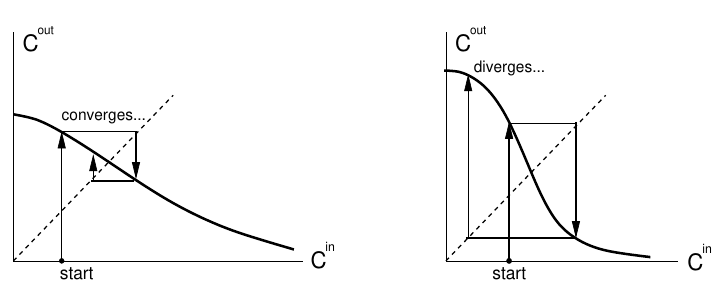
\includegraphics[scale=0.6]{figs/criterio.png}
	\legend{Fonte: \citeauthor{book_base}}
	\label{fig:criterio}
\end{figure}

Quando o sistema apresenta condições de contorno periódicas tais como sólidos, utiliza-se uma base que não depende das posições atômicas como a base \textit{"Ondas Planas"}. De modo geral, a expansão em Ondas Planas pode ser descrita da seguinte maneira:
\begin{equation}
	\varphi_i(\vb{r})=\frac{1}{\sqrt{\Omega}}\exp\bqty{i G_i\cdot \vb{r}}
\end{equation}

Por outro lado, ao realizar a expansão do orbital sobre um conjunto de funções de bases conhecidas, é possível realizar essa expansão de modo que essa base seja centrada em algum ponto do espaço. Para sistemas não periódicos, como moléculas, utiliza-se normalmente as bases centrada no núcleo denominada \textit{"Átomo-Centrada"}. As principais bases de átomo centrada são as bases \textit{Orbital do Tipo Slater} e \textit{Orbital do Tipo Gaussiana}. \cite{book_base}


\subsection{Orbital do Tipo Slater (STO)\label{sto}}

O conjunto de bases de átomo-centrada denominada \textit{Orbital do Tipo Slater} foi introduzida em 1930 pelo físico John C. Slater \cite{base_slater} e baseia-se na função de onda do átomo de hidrogênio, tendo sua forma dada por:
\begin{equation}
	\chi_{STO}(\vb{r}) = N r^{n-1}e^{\zeta r}\mathrm{Y}_{l,m}(\theta,\phi) \qquad n\in \mathbb{N}
\end{equation}

Onde \textit{r} é a distância dos elétrons ao núcleo atômico, \textit{n} representa o número quântico principal, $ \zeta $ é um parâmetro ajustável que representa a carga nuclear efetiva e \textit{N} é um fator de normalização. As bases do tipo STO formam um base de solução completa.

Uma característica dessa base é que ela não permite a estrutura de \textit{nós} assim como a solução do átomo de hidrogênio. Para permitir a estrutura de nós através dessa base é necessário uma combinação de várias bases STO. Nesse sentido, surge o conceito de \textit{Base Mínima}, ou seja a representação mais simples possível de um orbital atômico, como pode ser observado na Tabela . A base mínima contém uma função de base para cada orbital ocupado. Por outro lado, variando-se os valores do parâmetro $ \zeta $ é possível expandir a base mínima, de modo que essa nova base estendida é denominada "Duplo-Zeta", "Triplo-Zeta", etc. 
\begin{table}[H]
	\centering
	\caption{Tabela mostrando os orbitais dos elementos da tabela periódia em termos da Base Mínima e da Base Duplo-Zeta.}
	\begin{tabular}{ccc} 
		\hline\hline
		& Base Mínima         & Duplo-Zeta                  \\ \hline
		H, He               & 1s                  & 1s, 1s'                     \\
		Li $\rightarrow $ Ne & 1s, 2s, 2p          & 1s, 1s', 2s, 2s', 2p, 2p'   \\
		Na $\rightarrow $ Ar & 1s,$\ldots$, 3p, 3d & 1s, 1s', $\ldots$, 3d, 3d'  \\
		K $\rightarrow $ Kr  & 1s,$\ldots$, 4s, 4p & 1s, 1s',$\ldots$, 4p, 4p'   \\
		Rb $\rightarrow $ Xe & 1s,$\ldots$, 5s, 5p & 1s, 1s',$\ldots$, 5p, 5p'   \\
		\hline\hline
	\end{tabular}
	\legend{Fonte: \citeauthor{book_base}}
	\label{tab:base_minima}
\end{table}
A base STO converge rapidamente para o resultado quando aumenta-se o número de bases. No entanto, as integrais que envolvem a base STO são difíceis de resolver.
%
%\subsection{Orbital do Tipo Gaussiana (GTO)\label{gto}}
%
%A conjunto de bases denominada \textit{Orbital do Tipo Gaussiana} foi proposta em 1950 por Boys \cite{base_gauss}, sendo representada por:
%\begin{equation}
%	\chi_{GTO}= N r^{2(n-1)}e^{-\zeta r^2}\mathrm{Y}_{l,m}(\theta,\phi) \qquad n\in \mathbb{N}
%\end{equation}
%
%A base do tipo Gaussiana se destaca pela possibilidade de calcular as integrais analiticamente. A base GTO impõe uma restrição sobre as bases usadas, de modo que somente as funções de onda que obedeçam a $ l=n-1 $ são usadas, ou seja, 1s, 2p, 3d, $ \ldots$, mas não 2s, 3p, $\ldots  $ O conjunto de bases STO possui uma convergência melhor que o conjunto de bases GTO, uma vez que a GTO não representa de forma correta os comportamentos assintóticos da função de onda do um elétron, como pode ser observado na Figura \ref{fig:gto1} para o orbital 1s do átomo de hidrogênio. Por outro lado, é possível representar uma STO com uma combinação linear de GTO's, como mostra a Figura \ref{fig:gto2} no qual aproximou-se o orbital 1s por uma combinação linear de GTO.
%
%
%%
%%\begin{figure}[H]
%%	\centering
%%\subfig[Utilizando uma base GTO. Fonte: \cite{book_base}]{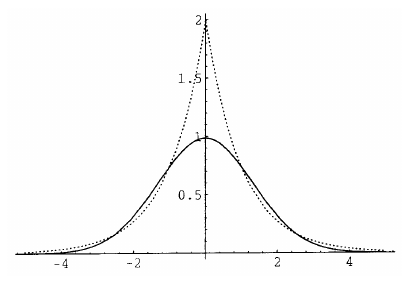
\includegraphics[scale=0.65]{figs/gtoh1.png}\label{fig:gto1}} \qquad
%%\subfig[Representação através de uma combinação linear de GTO's. Fonte: \cite{book_base}.]{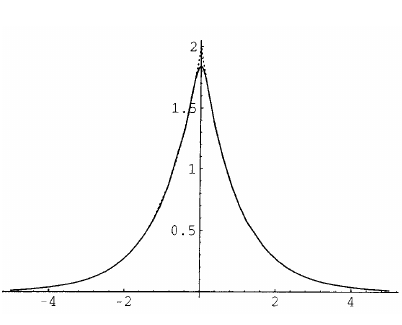
\includegraphics[scale=0.65]{figs/gto1sh1.png}\label{fig:gto2}}
%%	\caption{\textit{Representação do orbital 1s do átomo de hidrogênio (linha pontilhada) através da base GTO (linha contínua).}}
%%\end{figure}
%
%\begin{figure}[H]
%	\centering
%	\begin{subfigure}[b]{0.45\textwidth}            
%		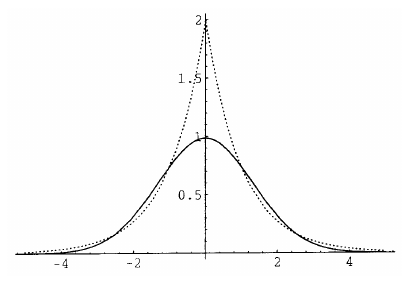
\includegraphics[width=\textwidth]{figs/gtoh1.png}
%		\caption{\textit{Representação usando uma base GTO. Fonte: \cite{book_base}}}
%		\label{fig:gto1}
%	\end{subfigure} \quad%
%	%add desired spacing between images, e. g. ~, \quad, \qquad etc.
%	%(or a blank line to force the subfigure onto a new line)
%	\begin{subfigure}[b]{0.37\textwidth}
%		\centering
%		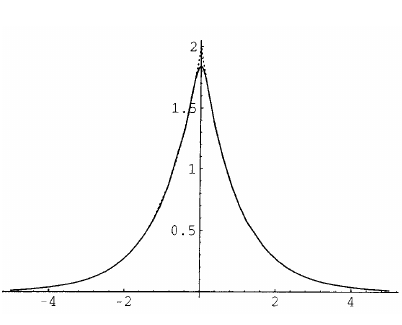
\includegraphics[width=\textwidth]{figs/gto1sh1.png}
%		\caption{\textit{Representação através de uma combinação linear de GTO's. Fonte: \cite{book_base}.}}
%		\label{fig:gto2}
%	\end{subfigure}
%	\caption{\textit{Representação do orbital 1s do átomo de hidrogênio (linha pontilhada) através da base GTO (linha contínua).}}\label{fig:gto}
%\end{figure}
\subsection{Orbital Atômico Numérico (NAO)}
Uma base atômica numérica- Numerical Atomic Orbital (NAO)-  é uma base estendida e localizada que reproduz a base minimal de forma continua, suave e diferenciável a partir de um raio de corte $r_m$. Essa base é representada por:
\begin{equation}
    \chi_{NAO}^I(\vb{r}_I)=\mathcal{R}^I_{nl}(r_I)\mathrm{Y}_{l,m}(\theta,\phi)
\end{equation}
onde, para cada átomo I, $\mathcal{R}^I_{nl}(r_I)$ é a função radial do n-ésimo orbital. 

A suavidade e o ajuste dessa base são definidos por um deslocamento de energia $\delta \epsilon$ (\textit{Energy Shift})  ganho devido ao confinamento dos orbitais em bases localizadas. Essa base apresenta uma melhor convergência com menos bases estendidas e corresponde ao tipo de base utilizada no código \textit{Siesta} \cite{nao}.

\section{Pseudopotenciais}

Devido à complexidade e ao custo computacional em um cálculo de muitos elétrons, é necessário utilizar aproximações que permitem modelar tais sistemas. Nesse sentido, o \textit{Método de Pseudopotencial} constitui uma importante ferramenta na otimização do custo computacional, uma vez que, substitui os efeitos dos elétrons do caroço por um potencial efetivo. Assim, nesse capítulo será apresentado os principais requisitos de um pseudopotencial.

O \textit{Método de Pseudopotencial}consiste em substituir os efeitos devido aos elétrons do caroço por um potencial efetivo, de modo a tratar somente os elétrons de valência. Os elétrons do caroço são aqueles mais próximos ao núcleo que não participam das ligações químicas. Assim, as propriedades químicas e físicas importantes em moléculas e materiais são determinadas pelos elétrons de valência \cite{tese_pseudo}. Nesse sentido, os estados dos elétrons do caroço são considerados como \textit{inertes}, de modo que através de um cálculo \textit{atômico} com todos os elétrons, obtém-se a forma espacial dos elétrons do caroço e considera-se que a função de onda dos elétrons do caroço permanece a mesma tanto para cálculos de moléculas, quanto para sólidos. A vantagem de substituir o potencial do núcleo por um potencial gerado pelo caroço reside no fato de que esse último é mais suave \cite{book_base}

A ideia de substituir o átomo por um caroço iônico que interage com os elétrons de valência, foi proposta inicialmente por E. Fermi em 1934 \cite{fermi}. Em 1935, Hellmann sugeriu a expressão abaixo para representar o potencial sentido pelos elétrons de valência do Potássio \cite{fermi_2}.
\begin{equation}
	w(r)=-\frac{1}{r}+\frac{274}{r}e^{-1.16r }
\end{equation}

No entanto, somente em 1959 com as contribuições de Phillips e Kleinman que os pseudopotenciais começaram a ser largamente utilizados \cite{pseudo_ref}. Com o advento e os avanços da Teoria do Funcional da Densidade, os pseudopotenciais passaram a ser gerados a partir da solução das Equações de Kohn-Sham para o problema atômico envolvendo todos os elétrons. \cite{toffoli_pseudo}

A construção de um pseudopotencial inicia com a escolha apropriada da configuração eletrônica do átomo, denominada \textit{configuração de referência}. Nessa etapa, separa-se na distribuição das camadas eletrônicas os elétrons do caroço e os elétrons de valência, além disso, acrescenta-se estados vazios aos estados dos elétrons de valência, a fim de incluir configurações iônicas. Outro requisito é que, a partir do ponto denominado \textit{Raio de Corte} $ r_c $, a função de onda de valência devido ao pseudopotencial seja igual a função de onda de valência obtida no cálculo com todos os elétrons \cite{book_base}. 

Na Figura \ref{fig:pseudo} está ilustrado o exemplo de um gráfico da função de onda em função do raio de corte para cada  valor do número quântico \textit{l} de uma determinada configuração iônica. Além disso, no gráfico está representado a função de onda correspondente ao cálculo com todos os elétrons realizados utilizando o funcional vdw-DF1 \cite{DRSLL}. Além disso, está representada a diferença existente entre os pseudopotenciais gerados pelo funcional GGA-PBE (\textit{PS-pbe}) e o funcional vdw-DF1 (\textit{PS-vdw}), junto aos respectivos raios de corte utilizados $ R_{pbe} $ e $ R_{vdw} $.
\begin{figure}[]
	\centering
	\caption{Gráfico da Função de Onda dos elétrons de valência da configuração de referência usada para o Paládio, calculados usando o funcional VDW-DRSLL e o funcional PBE. No gráfico está o cálculo com todos os elétrons e com o pseudopotencial em função do Raio.}	\label{fig:pseudo}
	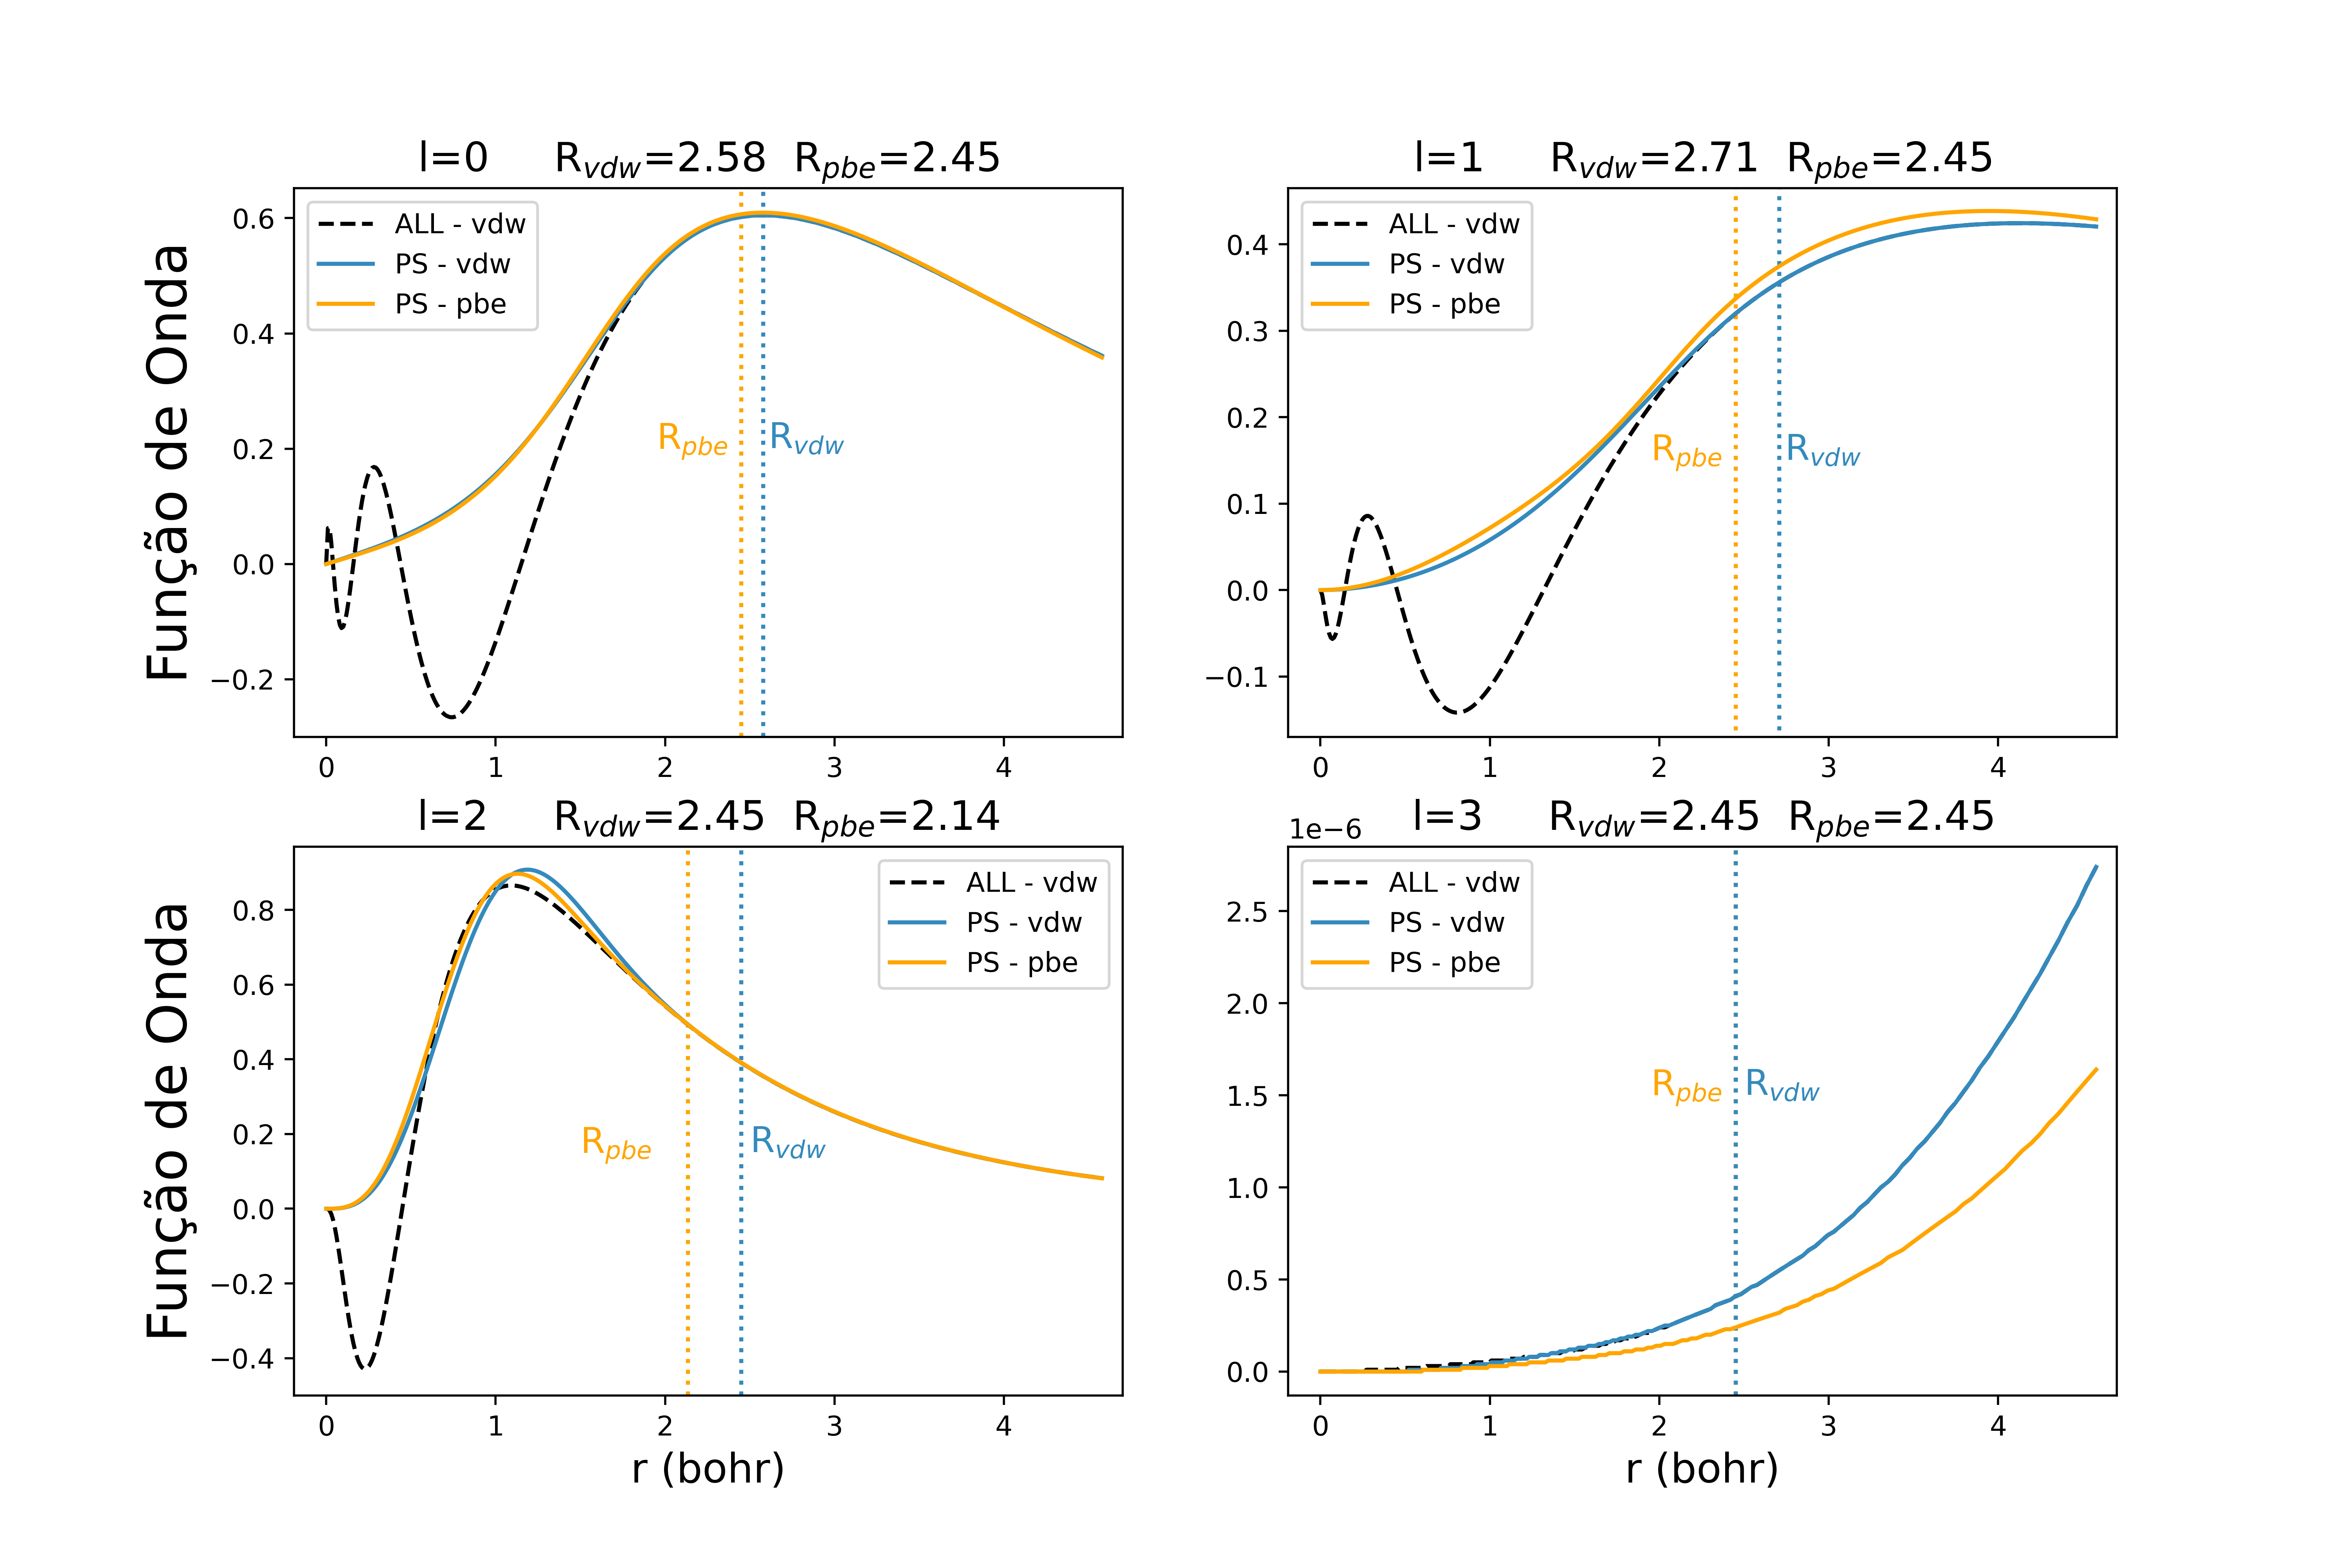
\includegraphics[scale=0.45]{figs/pseudo.png}
\legend{Fonte: Compilação da autora.}
\end{figure} 

Para encontrar as pseudofunções $ \varphi^{PS} $ geradas a partir do pseudopotencial, considere que as autofunções $ \Psi $ da Hamiltoniana $ \hat{H} $ é dada pela soma das autofunções do caroço $ \ket{\varphi_{c}} $ e de valência $ \ket{\varphi_{v}} $, tal que:
\begin{eqnarray}
	\hat{H}\ket{\psi_{c}}&=&\varepsilon_{c}\ket{\psi_{c}}\label{eq:caroco}\\
	\hat{H}\ket{\psi_{v}}&=&\varepsilon_{v}\ket{\psi_{v}}\label{eq:valencia}
\end{eqnarray}
Onde, foi utilizada a notação vetorial de Dirac. 

Supondo que a autofunção que corresponde ao pseudopotencial tem que ser uma função suave, então ela pode ser escrita em termos dos estados de valência $ \ket{\psi_{v}} $ e em termos da ortogonalização entre as autofunções de valência e as autofunções do caroço, tem-se:
%Supondo que, os orbitais de valência $ \ket{\psi_{v}} $ podem ser escritos em termos de uma função mais suave $ \ket{\varphi_v^{PS}} $, a função de onda gerada pelo pseudopotencial, somada à expansão dos orbitais de valência na base dos orbitais do caroço, tem-se a expressão abaixo \cite{pseudo_ref}.
\begin{equation}
	\ket{\varphi_v^{PS}}=\ket{\psi_{v}}+\sum_{c} \alpha_{cv}\ket{\psi_c}
\end{equation}
Onde,
\begin{equation}
	\alpha_{cv}=\braket{\psi_c}{\varphi_v^{PS}}
\end{equation}


Multiplicando por uma autofunção do caroço  $ \ket{\psi_{c'}} $ e integrando obtém-se os coeficientes $ \alpha_{cv} $:
\begin{equation}
	\braket{\psi_{c'}}{\varphi_v^{PS}}=\underbrace{\braket{\psi_{c'}}{\psi_{v}}}_{\substack{\text{= 0,}\\ \text{pois os estados de} \\ \text{valência e do}\\ \text{caroço pertencem} \\ \text{á mesma} \\ \text{Hamiltoniana}}}+\sum_{c}\alpha_{cv}\underbrace{\braket{\psi_{c'}}{\psi_{c}}}_{= \delta_{cc'}}
\end{equation}

A Equação de Schr$\"{o} $dinger para o a função de onda do pseudopotencial $  \ket{\varphi_v^{PS}}$ é dada por:
\begin{eqnarray}
	\hat{H}\ket{\varphi_v^{PS}}&=&\hat{H}\ket{\psi_{v}}+\sum_{c}\alpha_{cv} \hat{H}\ket{\psi_{c}} \\ \nonumber
	&=& \varepsilon_{v}\bqty{\ket{\varphi_v^{PS}}-\sum_{c} \alpha_{cv}\ket{\psi_c}}+\sum_{c} \alpha_{cv}\varepsilon_{c}\ket{\psi_{c}} \\ \nonumber
	&=& \varepsilon_{v}\ket{\varphi_v^{PS}}+\sum_{c}(\varepsilon_{c}-\varepsilon_{v})\alpha_{cv}\ket{\psi_{c}} 
\end{eqnarray}

Como $ \varepsilon_{v} $ é também autovalor de $ \ket{\varphi_v^{PS}} $, então a equação acima resulta em:
\begin{equation}\label{eq:pseudo}
	\bqty{\hat{H}+\sum_{c} (\varepsilon_{c}-\varepsilon_{v})\dyad{\psi_{c}}}\ket{\varphi_v^{PS}}=\epsilon_v\ket{\varphi_v^{PS}}
\end{equation}

Portanto, a \textit{Pseudo-Função de Onda} $ \ket{\varphi_v^{PS}} $ satisfaz a Equação de Schr$ \"{o} $dinger, cuja hamiltoniana é composta pela Hamiltoniana das Equações de Kohn-Sham, somada a uma pseudo-hamiltoniana dependente da energia. O segundo termo da equação \eqref{eq:pseudo} pode ser representado como um potencial repulsivo, pois o pseudopotencial é mais fraco que o potencial real na vizinhança do caroço. Assim reescrevendo a equação \eqref{eq:pseudo} em termos do \textit{Potencial Repulsivo} $ \hat{V}_R $, obtém-se:
\begin{equation}
	\pqty{\hat{H}+\hat{V}_R}\ket{\varphi_v^{PS}}=\epsilon_v\ket{\varphi_v^{PS}}
\end{equation} 

Como resultado, a pseudo função de onda $ \ket{\varphi_v^{PS}} $ satisfaz uma equação com um potencial efetivo $ \hat{V}_{R} $, cujo autovalor é o mesmo da autofunção real de valência $ \ket{\psi_{v}} $, equação \eqref{eq:valencia}. \cite{pseudo_ref}

A fim de obter pseudopotenciais mais suaves e precisos, em 1979 Hamann, Schlüter and Chiang \cite{pseudo_norma} sugeriram quatro critérios a serem cumpridos pelo pseudopontecial na configuração de referência, são as condições de \textit{Norma-Conservada} \cite{toffoli_pseudo}:
\begin{enumerate}
	\item Os autovalores correspondentes às pseudofunções $ \ket{\psi_{nl}^{PS}} $ tem que ser iguais aos autovalores da autofunções com todos os elétrons $ \ket{\psi_{nl}^{AE}} $ para a configuração de referência.
	\begin{eqnarray}
		\hat{H}\ket{\psi_{nl}^{AE}}&=&\varepsilon_{nl}\ket{\psi_{nl}^{AE}} \\ 
		\pqty{\hat{H}+\hat{V}_R}\ket{\psi_{nl}^{PS}}&=&\varepsilon_{nl}\ket{\psi_{nl}^{PS}}
	\end{eqnarray}
	\item As funções de onda do cálculo com todos os elétrons $ \psi_{nl}^{AE} $ tem que ser igual à função de onda gerada pelo pseudopotencial $\psi^{PS}_{nl}(\vb{r})$ a partir do ponto correspondente ao raio de corte $ r_c $.	
	\begin{equation}
		\psi^{AE}_{nl}(r)=\psi^{PS}_{nl}(r) \quad ,\forall \quad r\geq r_c 
	\end{equation}
	\item A densidade de carga da solução de todos os elétrons e para o pseudopotencial integradas no intervalo de 0 a \textit{R} devem ser iguais, para todo $ R\leq r_c $	
	\begin{equation}
		\int_{0}^{R}\abs{\psi^{AE}_{nl}(r)}^{2}r^2 dr=\int_{0}^{R}\abs{\psi^{PS}_{nl}(r)}^{2}r^2 dr
	\end{equation}
	\item A derivada logarítmica e a derivada da energia para ambos os casos tem que ser iguais para todo $ R\leq r_c $
	\begin{equation}
		\bqty{(r\psi^{AE}_{nl}(r))^2\dv{E}\dv{r}\ln \psi^{AE}_{nl}(r) }_{R}=\bqty{(r\psi^{PS}_{nl}(r))^2\dv{E}\dv{r}\ln \psi^{PS}_{nl}(r) }_{R}
	\end{equation}
\end{enumerate}

Em suma, a carga contida dentro do raio de corte é a mesma tanto para o pseudopotencial quanto para o cálculo com todos os elétrons \cite{book_base}.

Dentre as famílias de pseudopotenciais existentes, o pseudopotencial proposto por \textit{Troullier e Martins }\cite{troullier_martins} é um método eficiente, além de apresentar resultados mais suaves. O potencial de Troullier Martins fornece resultados mais precisos para os átomos com estados \textit{2p} de valência da primeira linha da tabela periódica, bem como para estados de valência \textit{d} dos metais de transição \cite{book_base}.

Nesse método, a parte radial da pseudo-funções de onda são definidas por:
\begin{equation}
	R_l^{PS}=\left\{\begin{matrix}
		R_{nl}^{AE}(r) & \text{, se} \quad r>r_c\\ 
		r^{l}e^{p(r)} &\text{, se}\quad r<r_c 
	\end{matrix}\right.
\end{equation}
onde,
\begin{equation}
	p(r)=c_0+c_2r^2+c_4r^4+c_6r^6+c_8r^8+c_{10}r^{10}+c_{12}r^{12}
\end{equation}

Os coeficientes de $ p(r) $ são ajustados a fim de cumprir as seguintes condições: manter a norma conservada; continuidade das funções de onda e da a primeira derivada em $ r=r_c $, não apresentar singularidades na origem; bem como obedecer à equação abaixo para os coeficientes \cite{pseudo_ref}.

\begin{equation}
	c_2^2+c_4(2l+5)=0
\end{equation} 
\chapter{Cálculos de Bulk e de Superfície dos Metais\label{apd:metal}}


\section{Paládio (Pd)}
\subsection{Bulk}
%Nos cálculos da estrutura bulk do Paládio foi utilizado uma \textit{base duplo-zeta polarizada} (DZP), no qual o momento angular dos elétrons de valência é descrito por duas funções radiais e uma função de polarização. Dessa forma,  para descrever os elétrons de valência, foi utilizado uma variação otimizadas da base DZP. Nesses cálculos o Método de Minimização utilizado foi o \textit{Gradiente Conjugado (CG)}, o critério de convergência utilizado foi da força $ 0,01$ eV/$\si{\angstrom}$ e o \textit{Mesh Cutoff} utilizado foi 400 Ryd. 

%Nesse sentido, para descrever os elétrons do caroço foi utilizado um pseudopotencial gerado com o funcional PBE com correção relativística e utilizando o Método de Norma Conservada de \textit{Troullier-Martins}. Os raios de corte estão descritos na Tabela \ref{tab:raios_corte} e a configuração de referência utilizada foi:
%As rotinas computacionais da primeira e segunda etapa foram executadas por meio do código \textit{Siesta} \cite{siesta} e a última, por meio do código \textit{Smeagol} \cite{smeagol1} \cite{smeagol2}. As coordenadas dos átomos que compõem as superfícies foram geradas por meio da biblioteca de ferramentas do \textit{Pyhton} denominada \textit{Atomic Simulation Environment} (ASE)\footnote[1]{Documentação do código: \url{https://wiki.fysik.dtu.dk/ase/}.} \cite{ase}. Os funcionais utilizados foram PBE \cite{PBE} e VDW-BH \cite{vdw-bh}

Os cálculos computacionais da estrutura \textit{bulk} do Paládio foram executados por meio do código \textit{Siesta} \cite{siesta}. Os funcionais de troca e correlação utilizados foram GGA-PBE \cite{PBE} e VDW-BH \cite{vdw-bh}. Além disso, utilizamos como método de minimização um algoritmo denominado \textit{Gradiente Conjugado (CG)} e  juntamente com o critério de convergência da força dado por $ 0.001$ eV/$\si{\angstrom}$, os pontos de corte da malha de integração do Siesta foram definidos com o tamanho da malha de 500 Ryd. A integração sobre os pontos do espaço recíproco seguiu o esquema proposto por \citeauthor{pontosk}, com os pontos k dados por $ 20\times20\times20 $ para os cálculos atômicos e de \textit{bulk}.  

Os elétrons de valência foram descritos por duas funções radiais e uma função de polarização, base denominada como \textit{duplo-zeta polarizada} (DZP). Dessa forma,  para descrever os elétrons de valência, utilizamos duas variações otimizadas da base DZP intituladas como DZP$^1$ e  DZP$^2$. Os parâmetros da base DZP$^1$ foram retirados do trabalho de \citeauthor{adrien} e da base DZP$^2$ do artigo de \citeauthor{pseudo_salvador}. 

Nesse sentido, para descrever os elétrons do caroço, utilizamos dois pseudopotenciais distintos obtidos a partir do Método de Norma Conservada de \textit{Troullier-Martins} com correção relativística. Em ambos pseudopotenciais, o cálculo com todos os elétrons foram executados utilizando o funcional PBE e foram denominados como \textit{PS-1} e \textit{PS-S}. O primeiro possui otimizações com correções não lineares no caroço e raios de corte $R_c$ sugeridos por \citeauthor{adrien} e o segundo por \citeauthor{pseudo_salvador}. Em ambos, a configuração de referência utilizada foi a distribuição eletrônica descrita abaixo, de modo que os raios de corte da base e do pseudopotencial, referentes aos respectivos níveis eletrônicos estão indicados na Tabela \ref{tab:raios_corte}.


\begin{equation}
	\bqty{Kr},5s^1,5p^0,4d^9,4f^0
\end{equation}

\begin{table}
	\centering
	\caption{Tabela contendo os valores dos raios de corte (bohr) de acordo com os níveis eletrônicos das bases DZP$ ^1 $ e DZP$ ^2 $ e dos pseudopotenciais PS-S e PS-1. \label{tab:raios_corte}}
	\begin{tabular}{clccccc} 
	\midrule\midrule
		\multicolumn{7}{c}{Raios de Corte -- Paládio}                                                        \\ 
		\midrule
		&  & \multicolumn{2}{c}{Base}            &  & \multicolumn{2}{c}{Pseudopotencial}  \\ 
		\midrule
		Nível Eletrônico &  & DZP$^{1}$ & DZP$^{2}$ &  & PS-S & PS-1                          \\ 
		\midrule
		5s               &  & 8.31/7.13        & 6.60/6.10        &  & 2.48 & 1.79                          \\
		5p               &  & 8.42             & 4.25             &  & 2.48 & 2.48                          \\
		4d               &  & 6.21/ 2.51       & 4.74/ 2.52       &  & 2.16 & 2.48                          \\
		4f               &  & -                & -                &  & 2.48 & 2.48                          \\
		\midrule\midrule
	\end{tabular}
\legend{Fonte: Compilação da autora.}
\end{table}


Os cálculos computacionais realizados pelo código Siesta fornecem informações atômicas e estruturais que podem ser comparadas aos valores obtidos experimentalmente, tais como parâmetro de rede, \emph{bulk modulus} e energia de coesão. O parâmetro de rede determina a distância interatômica na estrutura cristalina e é determinado de acordo com a configuração que fornece a energia mínima da estrutura \emph{bulk}. O \emph{bulk modulus} é uma medida de resistência em relação á compressão de uma substância. A energia de coesão de um cristal é definida como a energia que deve ser adicionada ao cristal a fim de separar sua estrutura em átomos neutros e livres, representada pela expressão \eqref{eq:ebulk}. \cite{kittel}

\begin{equation}\label{eq:ebulk}
	E_{coesão}=E_{sólido}-E_{átomo}
\end{equation}

Dessa forma, utilizando o funcional PBE, foram obtidos os parâmetros estruturais e eletrônicos do Pd \textit{bulk}: \textit{Parâmetro de rede} ($ \si{\angstrom} $), \textit{Bulk Modulus} (GPa) e \textit{Energia de Coesão} (eV), com as bases DZP$ ^1 $ e DZP$^2 $, junto com os pseudpotenciais \textit{PS-1} e \textit{PS-S}. Em posse desses resultados, verificou-se qual combinação de base e pseudopotencial que forneceram os valores mais próximos aos experimentais para o funcional PBE. 

Levando-se em consideração que o problema central desse trabalho é estudar a interface água/metal, é fundamental considerar as forças de dispersão de van der Waals \cite{vdw-func}. Nesse sentido, a fim de descrever e analisar essas interações, obtivemos as propriedades da estrutura bulk do Pd com o funcional de troca e correlação VDW-BH juntamente com a base e o pseudopotencial definidos via cálculos PBE. Isso foi feito pois a convergência do funcional PBE é mais rápida que a do funcional VDW-BH, além do fato de o PBE ser um funcional com resultados bem reportados na literatura \cite{adrien}. 

Os resultados obtidos computacionalmente para os parâmetros de interesse, bem como os valores experimentais estão descritos na Tabela \ref{tab:bulk}. Em relaçao ao \textit{Parâmetro de rede}, a base DZP$^2$ forneceu o valor mais próximo do valor experimental, cerca de $ 1.5\% $ maior, tanto para o pseudopotencial PS-S quanto para o PS-1; enquanto que, a base DZP$^1$ apresentou discrepâncias entre $ 2.3\% $ e $ 2.6\% $. No estudo conduzido por \citeauthor{pseudo_salvador}, onde foi apresentado o pseudopotencial PS-1 e base DZP$^2  $, o valor do parâmetro de rede para o Pd com o funcional PBE foi $ a_{salvador}=3.985\; \AA $, o que condiz com o nosso resultado. Da mesma forma, a base DZP$^2$ forneceu os valores do \textit{Bulk Modulus} mais próximos ao experimental para ambos os pseudopotenciais, com variações entre $6\%$ e $7\%$ menores.

Entretanto, para a \textit{Energia de Coesão} a base DZP$^1$ juntamente com o pseudopotencial PS-1 apresentou o resultado mais próximo ao experimental, com a discrepância de 10 $\%$; ao passo que a maior discrepância foi de $33\%$ dada pela base DZP$^2$+PS-S. \cite{vdw-article}. Dessa forma, escolhemos o a base DZP$^1$ e o pseudopotencial PS-1 para compor os cálculos com o funcional VDW-BH. O critério utilizado nessa escolha foi o valor da Energia de Coesão. Isso ocorreu pois estamos interessados no conjunto que forneça a energia mínima e que seja o mais próximo ao experimental. %Na Figura \ref{fig:fluxo} está representado um fluxograma sintetizando essa etapa do trabalho. 

%Bulk
\begin{table}[H]
	\centering
		\caption{Parâmetros estruturais obtidos com o funcional PBE de acordo com cada base, $DZP^1$ e $DZP^2$, junto a cada pseudopotencial PS-S e PS-1.\label{tab:bulk}}
	\begin{tabular}{ccccc} 
		\hline\hline\addlinespace[3.6pt]
		\multicolumn{5}{c}{\textbf{Valores dos parâmetros obtidos com o funcional PBE}}                                                        \\ \addlinespace[1.5pt]
		\midrule \addlinespace[1.5pt]
		\textit{Pseudo}       & \textit{Base}    & \textit{Par. de rede}$(\si{\angstrom})$ & \textit{Bulk Modulus} (GPa) & \textit{Energia de Coesão} (eV)  \\  
		\midrule
		\multirow{2}{*}{PS-S} &~~~DZP$^1$~~~& 3.98                          & 158 & 4.73          \\ \addlinespace[1pt]
		&~~~DZP$^2$~~~& 3.94                          & 183                      & 5.23                            \\ 
		\midrule
		\multirow{2}{*}{PS-1} &~~~DZP$^1$~~~& 3.97                          & 168                      & 4.34                            \\ 
		\addlinespace[1pt]
		&~~~DZP$^2$~~~& 3.94                          & 181                      & 4.85                            \\ \midrule	\multicolumn{5}{c}{\textbf{Valores dos parâmetros obtidos com o funcional VDW-BH}}    \\ \addlinespace[1pt]
		\midrule \addlinespace[3pt]
		PS-1 & DZP$ ^1 $&3.91 &199& 4.93                                                     \\ 
		\midrule
		\multicolumn{2}{c}{\textbf{Exp.}\tablefootnote[2]{CRC Handbook of Chemistry and Physics version 2008.}}        & \textbf{3.88}                          & \textbf{195}                     & \textbf{3.94}                             \\
		\hline\hline
	\end{tabular}
\legend{Fonte: Compilação da autora}
\end{table}



%\begin{figure}[H]
%	\centering
%	\includegraphics[scale=0.6]{figs/funcional.pdf}
%	\caption{\textit{Fluxograma ilustrando a escolha do pseudopotencial PS-1 e da base DZP$ ^1 $. Após obter os resultados com o funcional PBE e as diversas combinações, representado à esquerda, comparou-se com o valor experimental, escolhendo a combinação adequada para os cálculos VDW-BH (lado direito). Fonte: Compilação da autora.} }
%	\label{fig:fluxo}
%\end{figure}

Em relação aos valores obtidos com o funcional VDW-BH, é possível observar uma melhoria nos resultados obtidos para o pseudopotencial PS-1 e a base DZP$ ^1 $. Por exemplo, a discrepância do parâmetro de rede em relação ao valor experimental foi $ \delta_{PS-1}=0.03 \si{\angstrom}$, caracterizando uma redução de 0.06 em comparação ao funcional PBE. Além disso, no trabalho reportado por \citeauthor{vdw-bh}, o parâmetro de rede obtido com esse funcional para o Pd foi $ a_{vdw-BH}=3.89\si{\angstrom} $, próximo ao valor que obtivemos. Para o parâmetro bulk modulus, o valor obtido foi superior em 4 GPa em comparação ao valor experimental, o que indica uma melhor concordância do que o valor obtido por \citeauthor{vdw-bh} $ B_{vdw-bh}=207 $ GPa.  Por outro lado, para a energia de coesão a diferença foi 0.99 eV em relação ao valor experimental. Todavia, esse valor é da mesma ordem de grandeza do valor obtido no trabalho realizado por \citeauthor{vdw-article} com outro funcional da família vdW, dado por 4.37 eV.

Assim, de acordo com o critério de energia e após comparar bases e pseudopotenciais para a descrição da estrutura \textit{bulk} do Pd com o funcional PBE, obtemos que a base DZP$^1$ e o pseudopotencial PS-1 forneceram o menor valor da energia. Com esse conjunto, realizamos os cálculos com o funcional VDW-BH, cujo valor da energia de coesão foi maior que com PBE.


\subsection{Superfície}
A construção do modelo ideal de uma superfície pode ser pensado a partir de um cristal infinito em duas dimensões e finito ao longo da direção normal, no qual o arranjo atômico da estrutura cristalina \textit{bulk} é preservado; esse modelo é denominado \textit{bulk-terminated}. Para implementar esses modelos nos cálculos computacionais aplica-se as condições periódicas de contorno nas duas dimensões e, na direção normal, repete-se as camadas após uma camada de vácuo. Tal configuração é denominada por  \textit{slab}. 

Os cálculos de superfície do Pd foram realizados no código Siesta com os funcionais PBE e VDW-BH. O método de Minimização utilizado foi o CG com o critério da força dado por $ 0.001\;\text{eV}/\AA$ e o \textit{Mesh Cutoff} de 400 Ryd. Assim como no cálculo de \textit{bulk}, utilizou-se as bases DZP$ ^1 $ e DZP$^2  $ juntamente com os pseudopotenciais PS-S e PS-1 para os cálculos utilizando o funcional PBE. Em seguida, a partir dos resultados das combinações de bases e pseudopotenciais obtidos com o PBE, realizou-se os cálculos com o funcional VDW-BH.

Para descrever as superfícies de Pd, utilizamos duas estruturas \textit{slab}, cuja ordenação atômica da célula unitária era composta por $ 4\times 4\times 4$ e $ 6\times 6\times 4 $ átomos nas coordenadas \textit{x}, \textit{y} e \textit{z}, respectivamente,  e vácuo de $ 20\; \si{\angstrom}$. A orientação dos planos cristalográficos escolhida para as superfícies foi a orientação (111), uma vez que corresponde a orientação com a maior densidade de átomos. %As coordenadas atômicos foram geradas por meio da biblioteca de ferramentas do \textit{Pyhton} denominada \textit{Atomic Simulation Environment} (ASE)\footnote[1]{Documentação do código: \url{https://wiki.fysik.dtu.dk/ase/}.} \cite{ase}.  

Vale ressaltar que utilizamos diferentes tamanhos de células unitárias, pois os cálculos de energia total de sistemas periódicos utilizando condições periódicas de contorno são influenciados pelo tamanho da célula unitária. Em particular, para sistemas envolvendo a interface água/metal- tais como os que serão abordados na próxima sessão- a periodicidade imposta pode causar uma interação indesejada entre moléculas polares em células adjacentes, o que afeta tanto as energias, quanto as geometrias dos sistemas \cite{adrien}. Nesse sentido, considerando a adsorção de estruturas de água adsorvidas no Pd, nessa etapa foram analisados as propriedades de um slab de metal com dois tamanhos diferentes de células unitárias.

A grandeza física mensurada e analisada nessa etapa foi o valor da \textit{Função Trabalho} (W), de modo que, esse valor foi calculado para cada conjunto e para cada tamanho de superfície. A definição da Função Trabalho é a energia mínima necessária para remover um elétron do interior de um cristal para um ponto no vácuo sujeito ao campo eletrostático gerado pela superfície e é expressa por:
\begin{equation}\label{eq:work}
	W=-E_F+W_s
\end{equation}
onde $E_f$ é a \textit{Energia de Fermi} previamente calculada para um cristal infinito e $W_s$ é a energia de um elétron em repouso no vácuo e próximo à superfície.

Computacionalmente esse parâmetro é calculado a partir do arquivo de saída gerado pelo Siesta que contém as informações da energia potencial do cristal em cada ponto ao longo da direção normal \textit{z}. Assim, por meio do utilitário fornecido pelo Siesta, são obtidos os arquivos contendo a média planar e a média macroscópica da energia potencial, respectivamente de acordo com a expressões:
\begin{equation}\label{eq:planar}
	\bar{V}(z)=\frac{1}{S}\int_{S}\dd{x}\dd{y}V(\vb{r})
\end{equation}

\begin{equation}\label{eq:macro}
	\bar{\bar{V}}(z)\int \dd{z'}f(z-z')\bar{V}(z')
\end{equation}
onde $ f(z-z') $ é uma função de amortecimento suave dada por \footnote{Para mais detalhes, consultar \citeauthor{planar}.}  e:
\begin{equation}
	f(z-z')=\int \dd{z''}\omega_{l_1}(z-z'')\omega_{l_2}(z''-z')
\end{equation}

Na Figura \ref{fig:work1} está representado o potencial de uma superfície de tamanho  $4\times4\times4$ e o significado de \textit{W}. Além disso, é possível observar as alterações na Energia Potencial nos pontos correspondentes às posições dos átomos da superfície, bem como as distorções devido à quebra de simetria de um cristal \textit{bulk} para uma superfície presentes na camada próxima ao vácuo. Assim, utilizando a Equação \eqref{eq:work} e as curvas de potencial, foram obtidos os resultados de W para os diferentes funcionais, apresentados na Tabela \ref{tab:work}. 

Considerando as bases DZP$^1  $ e DZP$ ^2 $, tem-se que os valores mais próximos à função trabalho experimental do Pd (111) foram obtidos para a base DZP$^1$, com ênfase para o pseudopotencial PS-1, cujas discrepâncias foram $\delta_{4\times4\times4}=0.30$ eV e $\delta_{6\times6\times4}=0.32$ eV. Por outro lado, a base DZP$^2$ forneceu resultados divergentes do experimental, com discrepâncias variando entre 1.4 a 1.8 eV. Os valores obtidos com a base DZP$ ^1 $ e o pseudopotencial PS-1 para o funcional PBE estão de acordo com o valor obtido por \citeauthor{work} para o Pd - fcc(111)- com esse funcional, $ W_{ref}=5.32 $ eV.
\begin{table}[h!]
	\centering
		\caption{Tabela contendo os valores obtidos para a Função Trabalho em elétron-Volt (eV).\label{tab:work}}
	\begin{tabular}{cccc} 
		\hline\hline\addlinespace[3.6pt]
		\multicolumn{4}{c}{\textbf{Funcional PBE}}                                                                                         \\ \addlinespace[2pt]
		\midrule \addlinespace[2pt]
		\textit{Pseudopotencial} & Base                                                               & Superfície        & Função Trabalho (eV)  \\ 
		\midrule
		\multirow{4}{*}{PS-S}    & \multirow{2}{*}{DZP$^1$}                                           & $4\times4\times4$ & 5.15                 \\ 
		\cdashline{3-4}[1pt/1pt] \addlinespace[3pt]
		&                                                                    & $6\times6\times4$ & 5.13                 \\ 
		\cmidrule{2-4}
		& \multirow{2}{*}{DZP$^2$}                                           & $4\times4\times4$ & 3.87                 \\ 
		\cdashline{3-4}[1pt/1pt]\addlinespace[3pt]
		&                                                                    & $6\times6\times4$ & 3.80                 \\ 
		\midrule
		\multirow{4}{*}{PS-1}    & \multirow{2}{*}{\begin{tabular}[c]{@{}c@{}}DZP$^1$\\\end{tabular}} & $4\times4\times4$ & 5.30                 \\ 
		\cdashline{3-4}[1pt/1pt]\addlinespace[3pt]
		&                                                                    & $6\times6\times4$ & 5.28                 \\ 
		\cmidrule{2-4}
		& \multirow{2}{*}{DZP$^2$}                                           & $4\times4\times4$ & 4.19             \\ 
		\cdashline{3-4}[1pt/1pt]\addlinespace[3pt]
		&                                                                    & $6\times6\times4$ & 4.15                 \\ 	\hline\addlinespace[3pt]
		\multicolumn{4}{c}{\textbf{Funcional VDW-BH}}                                                                                         \\
		\midrule
		\multirow{2}{*}{PS-1}    & \multirow{2}{*}{\begin{tabular}[c]{@{}c@{}}DZP$^1$\\\end{tabular}} & $4\times4\times4$ & 5.43                 \\ 
		\cdashline{3-4}[1pt/1pt]\addlinespace[3pt]
		&                                                                    & $6\times6\times4$ &     5.46           \\ 
		\midrule
		\multicolumn{3}{c}{\textbf{Exp.}\tablefootnote[2]{CRC Handbook of Chemistry and Physics version 2008, p. 12–114.}}                                                                                          & \textbf{5.60}                 \\
		\hline\hline
	\end{tabular}
	\legend{Fonte: Compilação da autora}
\end{table}
\begin{figure}[h!]
	\centering
	\caption{Curva de energia potencial pela distância no eixo z de uma superfície de Pd de tamanho $4\times4\times4$. No gráfico $ E_f $ corresponde à Energia de Fermi do sistema e W é a função trabalho; as linhas tracejadas representam a caixa unitária.}
	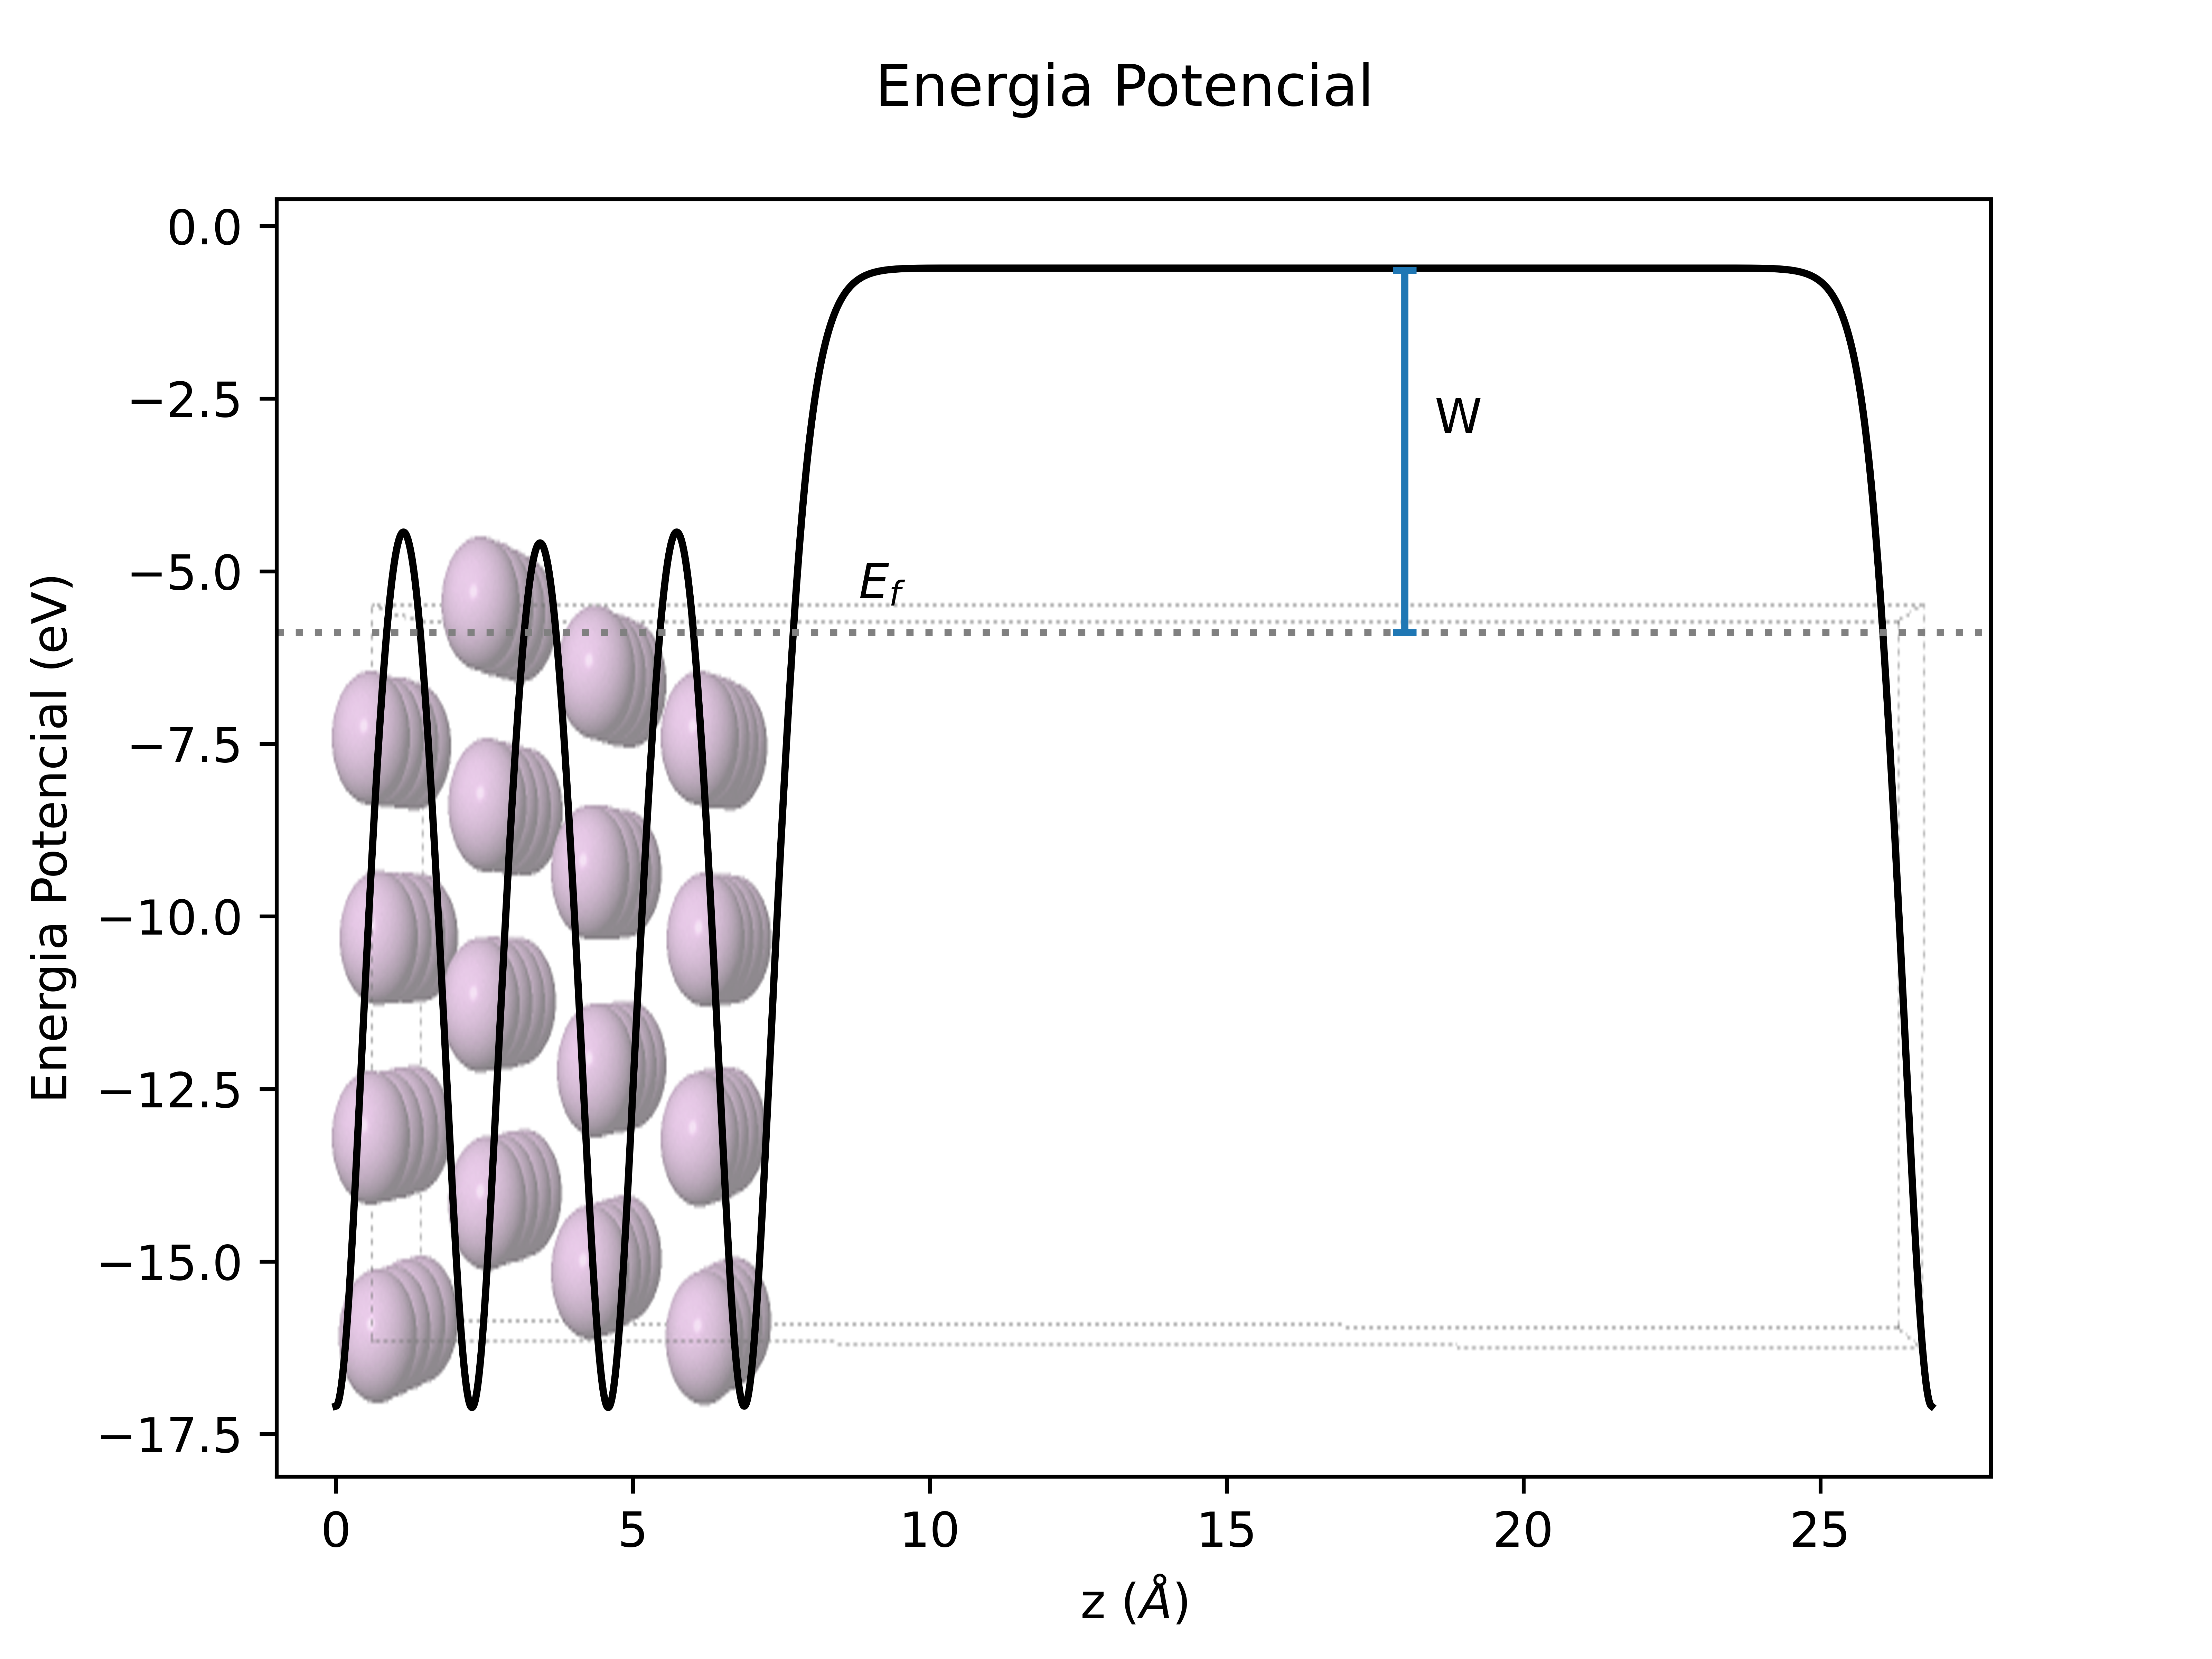
\includegraphics[scale=0.8]{figs/work2.png}
	\legend{Fonte: compilação da autora.}
	\label{fig:work1}
\end{figure}

Assim como para o cálculo de bulk, os valores obtidos com o pseudopotencial PS-1 e base DZP$ ^1 $ com o funcional PBE foram os mais próximos ao experimental, de modo que os cálculos envolvendo o funcional VDW-BH foram realizados com esse conjunto de descritores. Comparando com os valores obtidos via PBE, observa-se uma melhoria nos valores fornecidos pelo funcional VDW-BH com os resultados mais próximos ao experimental cujas discrepâncias foram $\delta_{4\times4\times4}=0.17$ eV e $\delta_{6\times6\times4}=0.14$ eV.



Portanto, a partir da caracterização do Pd é possível concluir que o funcional VDW-BH fornece resultados melhores que o funcional PBE em alguns resultados analisados. Isso constitui uma vantagem, visto que é esperado que esse funcional seja mais sensível às interações água-Pd, corroborando assim para a descrição posterior da água adsorvida no metal. Além disso, a partir dos resultados obtidos nessa etapa, definiu-se o conjunto de base e pseudopotencial que melhor descrevem as propriedades eletrônicas e estruturais do paládio, tanto para a estrutura \textit{bulk}, quanto para a estrutura \textit{slab}. 


\section{Raios de Corte}
Para descrever as moléculas de água durante as simulações foi utilizado bases DZP e pseudpotenciais de norma conservada de acordo com a norma de \textit{Troulier-Martins}. Assim, os raios de corte do oxigênio e do hidrogênio estão descritos nas Tabelas \ref{tab:o} e \ref{tab:h}, respectivamente. Além disso, foi investigado o efeito do potencial sobre eletrodos metálicos de ouro, cujos raios de corte estão descritos na Tabela \ref{tab:au}. Nas simulações com a superfície metálicas de Au, foi utilizado a base DZP$ ^{Au} $ para descrever os eletrodos e a base DZP$^{Aus}  $ para descrever a região de espalhamento.

\begin{table}[H]
	\centering
		\caption{Raios de Corte (bohr) da base DZP e do pseudopotencial utilizados para descrever os átomos de oxigênio.\label{tab:o}}
	\begin{tabular}{clccc} 
		\hline\hline
		\multicolumn{5}{c}{Raios de Corte - Oxigênio (O)}          \\ 
		\midrule
		Nível Eletrônico &  & DZP &  & Pseudopotencial  \\ 
		\midrule
		2s               &  & 4.51/2.64  &  & 1.14             \\
		2p               &  & 6.15/2.59  &  & 1.14             \\
		3d               &  & 3.54       &  & 1.14             \\
		4f               &  & -          &  & 1.14             \\
		\hline\hline
	\end{tabular}
\end{table}

\begin{table}[H]
	\centering
			\caption{Raios de Corte (bohr) da base DZP e do pseudopotencial utilizados para descrever os átomos de hidrogênio.\label{tab:h}}
	\begin{tabular}{clccc} 
		\hline\hline
		\multicolumn{5}{c}{Raios de Corte - Hidrogênio (H)}    \\ 
		\midrule
		Nível Eletrônico &  & DZP &  & Pseudopotencial  \\ 
		\midrule
		1s               &  & 4.20/1.84  &  & 1.25             \\
		2p               &  & 3.52       &  & 1.25             \\
		3d               &  & -          &  & 1.25             \\
		4f               &  & -          &  & 1.25             \\
		\hline\hline
	\end{tabular}
\end{table}

\begin{table}[H]
	\centering
	\caption{Raios de Corte (bohr) da base DZP e do pseudopotencial utilizados para descrever os átomos de ouro.\label{tab:au}}
	\begin{tabular}{clcccc} 
		\hline\hline
		\multicolumn{6}{c}{Raios de Corte - Ouro (Au)}                                                \\ 
		\midrule
		\multicolumn{1}{l}{Nível Eletrônico} &  & DZP$^{Au}$ & DZP$^{Aus}$ &  &      Pseudopotencial             \\ 
		\midrule
		6s                                   &  & 7.25/5.79  & 9.08/5.79   &  & 2.32             \\
		6p                                   &  & -          & -           &  & 2.29             \\
		5d                                   &  & 5.11/2.87  & 6.56/2.87   &  & 2.24             \\
		5f                                   &  & -          & -           &  & 2.00             \\
		\hline\hline
	\end{tabular}
\end{table}


%\chapter{Cálculo de Superfícies}

O estudo da composição química e do arranjo atômico da superfície de um sólido permite determinar as propriedades mecânicas, elétricas e químicas de um material e possui aplicações práticas em processos de catálise, na fabricação de interfaces e membranas, além de fornecer importantes resultados na fabricação de semicondutores \cite{density-book}.

Dessa forma, na Seção \ref{slab} será apresentado o modelo computacional de uma superfície: \textit{o modelo de slab}. Além disso, serão estudadas as orientações cristalográficas de uma superfície construída a partir de uma estrutura \textit{fcc}. Na Seção \ref{work} será estudado o conceito de \textit{Função Trabalho}.
\section{Construção e Orientação de uma Superfície\label{slab}}

A construção do modelo ideal de uma superfície pode ser pensado a partir de um cristal infinito em duas dimensões e finito ao longo da direção normal, no qual o arranjo atômico da estrutura cristalina \textit{bulk} é preservada; esse modelo é denominado \textit{bulk-terminated}. Por outro lado, ao modelar uma superfície real deve-se levar em conta que, quando a periodicidade da rede cristalina é quebrada, os átomos que estão próximos à superfície estão sujeitos à forças diferentes daquelas que atuavam no interior do cristal. Isso leva os átomos a se rearranjarem e ocuparem novas posições de equilíbrio, diferentes das posições da estrutura bulk. % O rearranjo atômico por relaxação corresponde à diminuição da distância  interplanar entre a primeira e a segunda camada, conservado-se a simetria original paralela à superfície \textit{bulk-terminated}. No processo de reconstrução os átomos se posicionam em uma simetria e orientação diferente da original \cite{surface-book}. Na Figura \ref{fig:relaxacao} está ilustrado a diferença das posições atômicas em cada arranjo para uma estrutura fcc cuja orientação original corresponde a (110).

Para implementar esses modelos nos cálculos computacionais aplica-se as condições periódicas de contorno nas duas dimensões e na direção normal repete-se as camadas após uma camada de vácuo, essa configuração é denominada \textit{slab} e está ilustrado na Figura \ref{fig:slab1}. Assim, nesse modelo forma-se várias camadas de superfície separadas por espaços vazios, como pode ser visto na Figura \ref{fig:slab2}. Nesse sentido, para obter uma descrição mais realística possível através do modelo slab, é necessário que o tamanho do vácuo seja largo o suficiente para que a densidade eletrônica do material tenda a zero no vácuo e não influencie os átomos da próxima camada e que as camadas sejam finas o bastante para modelar a superfície \cite{density-book}.
%\begin{figure}[H]
%	\centering
%	\includegraphics[scale=0.45]{figs/relaxacao.png}
%	\caption{\textit{Modelo ideal de uma superfície fcc de orientação (100). Fonte: Adaptado de \cite{surface-book}}}
%	\label{fig:relaxacao}
%\end{figure}



\begin{figure}
	\centering
	\begin{subfigure}[b]{0.4\textwidth}            
		\includegraphics[scale=0.5]{figs/slab1.jpg}
		\caption{\textit{Exemplo de uma célula unitária que compõe a superfície de um sólido. Fonte: \citeauthor{density-book}}}
		\label{fig:slab1}
	\end{subfigure}\;\;
	%add desired spacing between images, e. g. ~, \quad, \qquad etc.
	%(or a blank line to force the subfigure onto a new line)
	\begin{subfigure}[b]{0.4\textwidth}
		\centering
		\includegraphics[scale=0.4]{figs/slab4.png}
		\caption{\textit{Ilustração do modelo de superfície de um sólido, no qual se aplica as condições de contorno nas três dimensões. Fonte: \citeauthor{surface-book}.}}
		\label{fig:slab2}
	\end{subfigure}
	\caption{\textit{Ilustrações do modelo slab de uma superfície.}}\label{fig:slab}
\end{figure} 

Dentre as diversas maneiras de rearranjar os átomos de uma superfície, deve-se levar em conta os diferentes planos cristalográficos de um cristal, ao longo dos quais revelam distintas posições atômicas de uma superfície. Dessa forma, a notação que descreve os planos cristalográficos de um cristal é dado pelos \textit{Índices de Miller} \cite{density-book}. 

A orientação de um plano cristalográfico é dado pela direção do vetor normal $ \vb{n} $ à esse plano. O vetor $ \vb{n} $ é dado em termos dos vetores de base $ \Bqty{\vb{g}_i}_{i=1}^{3} $ do espaço recíproco $ \vb{n}=h\vb{g}_1+k\vb{g}_2+l\vb{g}_3 $. Na notação dos índices de Miller o vetor normal é descrito por: $ \bqty{hkl} $, ao passo que a orientação do plano cristalino é identificada pela notação $ (hkl) $ \cite{surface-book}.

%Os índices de Miller de uma plano cristalográfico podem ser definidos a partir dos vetores do espaço real, para isso basta especificar os pontos no qual o plano intersecta alguns dos três eixos do cristal e em seguida, tomar o inverso dos valores do conjunto de pontos, que correspondem aos respectivos pontos no espaço recíproco. 

%Na Figura \ref{fig:100-plane} está ilustrado o plano (001) de uma estrutura cristalina \textit{cúbica de face centrada} (fcc); analisando a figura, nota-se que o plano intersecta somente o eixo \textit{z}, de modo que, o valor dos pontos de interseção no espaço recíproco equivale a $ \pqty{\frac{1}{\infty},\frac{1}{\infty},1} $, resultando na identificação (001). Se o plano intersecta o eixo \textit{x, y} e \textit{z} nos respectivos pontos iguais a 1, então a identificação do plano é (111). 

%\begin{figure}[H]
%	\centering
%	\begin{subfigure}[b]{0.4\textwidth}       %     
	%		\includegraphics[scale=1.15]{figs/fcc.png}
	%		\caption{\textit{Ilustração do plano cristalográfico (001) de uma estrutura fcc. Fonte: \citeauthor{density-book}}}
	%		\label{fig:100-plane}
	%	\end{subfigure}\;\;
%add desired spacing between images, e. g. ~, \quad, \qquad etc.
%(or a blank line to force the subfigure onto a new line)
%	\begin{subfigure}[b]{0.4\textwidth}
	%		\centering
	%		\includegraphics[scale=0.4]{figs/fcc2.png}
	%		\caption{\textit{Ilustração do plano cristalográfico (111) de uma estrutura fcc. Fonte: \citeauthor{density-book}.}}
	%		\label{fig:111-plane}
	%	\end{subfigure}
%	\caption{\textit{Planos cristalográficos %de uma estrutura fcc}}\label{fig:plane}
%\end{figure} 

Aém disso, a densidade de átomos em uma superfície varia de acordo com a orientação. Como por exemplo, para uma estrutura cúbica de face centrada, a orientação de maior densidade é (111). Isso é importante, pois geralmente, a superfície construída com a orientação cristalográfica que abrange a maior densidade de átomos é mais estável \cite{density-book}. Essa colocação pode ser ilustrada a partir da visão frontal das posições atômicas, exibida na Figura \ref{fig:top}. Além disso, é possível identificar simetrias de rotação existentes em cada orientação \cite{density-book}.  
\begin{figure}[H]
	\centering
	\includegraphics[scale=0.5]{figs/top-view.png}
	\caption{\textit{Vista frontal da posição dos átomos de uma superfície de orientação (100), (111) e (110). Fonte: \citeauthor{density-book}}.}
	\label{fig:top}
\end{figure}
\section{Função Trabalho\label{work}}
A \textit{função trabalho} é definida como a energia mínima necessária para remover um elétron do interior de um sólido. Além disso, constitui um importante conceito para o estudo de metais. O valor da função trabalho depende das propriedades da superfície e das características do interior do sólido, uma vez que existem distorções na distribuição da carga eletrônica na superfície que afetam níveis eletrônicos distantes. Esses efeitos são fundamentais para descrever fenômenos como emissão termiônica, efeito fotoelétrico, potencial de contato e qualquer outro fenômeno no qual os elétrons sejam extraídos de uma superfície.  

Os efeitos da quebra de simetria de um cristal infinito e como isso afeta a energia necessária para remover um elétron podem ser ilustrados por meio de uma comparação qualitativa entre o potencial periódico de um cristal infinito $V^{inf}(\vb{r}) $, com o potencial $ V^{fin}(\vb{r}) $ de um cristal finito. Assim, em um estrutura cristalina infinta, o potencial $ V^{inf}(\vb{r}) $ pode ser representado como a soma das contribuições da célula primitiva de \textit{Wigner-Seitz}\footnote{\textit{Célula primitiva de Wigner-Seitz: é a célula primitiva que mantém a simetria completa da rede cristalina \cite{estado-solido2}.}} sobre cada ponto do cristal à uma distância $ \vb{R} $, tal que a expressão seja dada por: 
\begin{equation}\label{eq:v-inf}
	V^{inf}(\vb{r})=\sum_{\vb{R}}v(\vb{r}-\vb{R})
\end{equation}
Considerando que, o potencial da célula primitiva sobre cada ponto do cristal seja dado pelo potencial de Hartree, então:
\begin{equation}
	v(\vb{r})=-e\int_C \dd{\vb{r'}}\denslinha\frac{1}{\vqty{\vb{r}-\vb{r'}}}
\end{equation}
onde, a integral é realizada sobre a célula primitiva e $ \dens $ é a densidade de carga eletrônica. Assim, o efeito do potencial periódico dado pela Equação \eqref{eq:v-inf} a uma distância muito longa ($ r'\gg r $) pode ser escrito em termos da expansão multipolar:
\begin{eqnarray}
	\frac{1}{\vqty{\vb{r}-\vb{r'}}}&=&\frac{1}{r}-(\vb{r'}\cdot\grad)\frac{1}{r}+\frac{1}{2}(\vb{r'}\cdot\grad)^2\frac{1}{r}+\ldots \nonumber\\ &=&\frac{1}{r}+\frac{\vb{r'}\cdot\vu{r}}{r^2}+\frac{3\pqty{\vb{r'}\cdot\vu{r}}^2-r'^2}{r^3}+\frac{1}{r}\mathcal{O}\pqty{\frac{r'}{r}^3}
\end{eqnarray}
resultando na seguinte expressão:
\begin{equation}\label{eq:v-expan}
	v(\vb{r})=-e\frac{Q}{r}-e\frac{\vb{p}\cdot\vu{r}}{r^2}+\mathcal{O}\pqty{\frac{1}{r^3}}
\end{equation}
Onde \textit{Q} é a carga total e $ \vb{p} $ é o momento de dipolo total, definidos por:
\begin{equation}
	Q=\int_{C}\dd{\vb{r'}}\denslinha\qquad \vb{p}=\int_{C}\dd{\vb{r'}}\vb{r'}\denslinha
\end{equation}
Analisando a Equação \eqref{eq:v-expan}, tem-se que $ Q=0 $, porque o cristal é eletricamente neutro e $ \dens $ possui a periodicidade da rede, logo cada célula primitiva é também eletricamente neutra. Além disso, como a estrutura cristalina considerada é infinita, então, devido às simetrias de inversão e cúbica, o momento de dipolo $ \vb{p} $, de quadrupolo e o termo de $ \frac{1}{r^4}$ também se anulam. Portanto, a contribuição da célula de Wigner-Seitz para $ v(\vb{r}) $ decresce com $ \frac{1}{r^5} $, ou seja, muito rápido para longas distâncias. Nesse sentido, em um cristal infinito, a contribuição de $ V^{inf}(\vb{r}) $ para longas distâncias é desprezível, de modo que a distribuição de carga não sofre distorções em nenhum ponto do cristal \cite{ashcroft}. 

Por outro lado, quando um elétron é retirado de um cristal finito, na região próxima à superfície do cristal terá distorções na densidade de carga eletrônica em comparação à distribuição de carga no interior do cristal. Essas distorções estão ilustradas na Figura \ref{fig:trabalho}. Isso ocorre pois, após a retirada do elétron, as posições atômicas podem assumir novas configurações de equilíbrio que diferem das posições no interior do cristal; o rearranjo atômico vai depender das simetrias na superfície e das orientações dos planos cristalográficos. Ademais, devido à quebra de periodicidade em um cristal finito, o momento de dipolo $ \vb{p} $ próximo à superfície não é nulo, de modo que, podem surgir cargas superficiais. 

Desse modo, considera-se primeiramente distorções da superfície que não induzem uma carga macroscópica líquida por unidade de área em uma superfície metálica, no qual o metal como um todo seja eletricamente neutro. Assim, a longas distâncias da superfície eletricamente neutra, tem-se que as distribuições de carga das células individuais distorcidas não produzirão campos elétricos macroscópicos líquidos. No entanto, dentro das camadas que compõe a superfície e que apresentam as distorções de carga, é induzido um campo elétrico $ \vb{E_s} $, de modo que, para mover um elétron através de uma camada é necessário executar um trabalho correspondente a $ W_s=e\int\vb{E_s}\cdot \dd{\vb{l}} $.

O valor de $ W_s $ depende do tipo de superfície e também da maneira pela qual as características da superfície diferem do bulk. Em alguns modelos, a distorção de carga da superfície é representada como uma densidade uniforme superficial macroscópica de dipolos, de modo que a camada da superfície é denominada \textit{dupla camada}. Logo, a energia mínima necessária para remover um elétron do interior de um cristal para uma ponto fora do cristal é dado por:
\begin{equation}
	W=-E_F+W_s
\end{equation}
Onde $E_f$ é a \textit{Energia de Fermi}, previamente calculada para um cristal infinito \cite{ashcroft}. Na Figura \ref{fig:trabalho} está ilustrado a forma do potencial $ V $ na superfície de um cristal. 


\begin{figure}[H]
	\centering
	\includegraphics[scale=0.6]{figs/trabalho.png}
	\caption{\textit{(a) Gráfico da densidade de carga elétrica próxima à superfície ideal de um cristal finito, no qual aparece as distorções.  As linhas tracejadas indicam as condições de contorno periódicas no interior do sólido. (b) Gráfico do potencial do cristal após aconteces as distorções descritas em (a). No gráfico está ilustrado o trabalho necessário $ W $ para retirar um elétron do campo elétrico da superfície. Fonte: \citeauthor{ashcroft}}}
	\label{fig:trabalho}
\end{figure}

%\section{Modos Normais de Vibração}


\end{apendicesenv}
%% ---
%
%
%% ----------------------------------------------------------
%% Anexos
% ----------------------------------------------------------

% ---
% Inicia os anexos
% ---
%\begin{anexosenv}

% Imprime uma página indicando o início dos anexos
%\partanexos

%\include{texto/anexo-2}

%\include{texto/anexo-1}

%\end{anexosenv}

%---------------------------------------------------------------------
% INDICE REMISSIVO
%---------------------------------------------------------------------

%\printindex


\end{document}

